%\documentclass[11pt,a4paper]{book} % double-sided
\documentclass[12pt,a4paper]{report}

\usepackage{subfigure,epsfig,amstext,floatfig,alltt,fancyhdr,setspace}
\usepackage{amsmath, slashed, amsfonts, mathtools}

\include{macros}
\initfloatingfigs

%%% helps to discourage hyphenation 10000 for no hyphens but dodgy line lengths%%%
\hyphenpenalty=5000
\tolerance=1000

%%%%%%% FINAL THESIS MARGINS  %%%%%%%%%
\setlength{\oddsidemargin}{1.46cm}
\setlength{\evensidemargin}{-0.04cm}
\setlength{\textwidth}{14.5cm}
\setlength{\topmargin}{-0.54cm}
\setlength{\textheight}{21.9cm}
\renewcommand{\hoffset}{0cm}
\renewcommand{\voffset}{0cm}
%%%%%%%%%%%%%%%%%%%%%%%%%%%%%%%%%%%%%%%

% Hack to avoid 'noindent'-ing everywhere
% \setlength{\parindent}{0pt}

%% In the beginning ....
\begin{document}

%% First do introductory stuff - leave this as pagestyle empty until after
%% the table of contents
%\pagestyle{empty}
%\title{
\pagestyle{empty}

\begin{center}

\LARGE

{\bf High Energy Resummation at Hadronic Colliders}

\vspace{1cm}

\begin{figure}[ht]
\begin{center}

\epsfig{file=crest.eps,width=0.3\linewidth}
\end{center}
\end{figure}

\large

{\it Jack J. Medley}

\vspace{2cm}
\normalsize
%\begin{center}
A thesis submitted in fulfilment of the requirements\\
for the degree of Doctor of Philosophy\\
to the\\
University of Edinburgh

March 2016
\end{center}


%\ \newpage		% Newpage needed if doing double sided.

%% Include abstract - use separate parskip for this and then set parskip for
%% rest of thesis.
%\pagestyle{plain}

% Jacks extra definitions
\newcommand{\bk}[3]{
	\langle #1 | #2 | #3 \rangle
}

\newcommand{\zg}[0]{{Z/\gamma^*}}

\newcommand{\lr}[1]{
	\langle #1 \rangle
}
\newcommand{\rl}[2]{
	|#1 \rangle\langle #2|
}
\newcommand{\gu}[1]{
	\gamma^{#1}
}
\newcommand{\gl}[1]{
	\gamma_{#1}
}
\newcommand{\lspin}[3]{
	\overline{#1}_{#2}^{#3}
}
\newcommand{\rspin}[3]{
	{#1}_{#2}^{#3}
}
\newcommand{\half}[0]{
	\frac{1}{2}
}

%-----------------------------------------------------------------------------

\pagestyle{fancy}
\fancyhead{} %clear all fields
\renewcommand{\headheight}{28pt}
\cfoot{}
\fancyfoot[LE,RO]{\thepage}

\renewcommand{\chaptermark}[1]{\markboth{\chaptername \ \thechapter.\ #1}{}}
\renewcommand{\sectionmark}[1]{\markright{\thesection.\ #1} {}}

\fancyhead[LE]{\small \slshape \leftmark}       % Chapter in the right on even pages
\fancyhead[RO]{\small \slshape \rightmark}      % Section in the left on odd pages
\renewcommand{\headrulewidth}{0.3pt}    	% Width of head rule

%-----------------------------------------------------------------------------

\pagenumbering{roman}
\setcounter{page}{1}

\onehalfspacing

\addcontentsline{toc}{chapter}{Abstract}
\chapter*{Lay Summary}
\noindent
	At experiments like the Large Hadron Collider (LHC) we seek to explore new areas of particle
	physics by accelerating hadrons (such as protons) into one another.  Because hadrons are
	comprised of more fundamental particles, namely; quarks, anti-quarks and gluons, what we
	see after these collisions is the result of two (or more) of these particles
	scattering off each other.  We use a Relativistic Quantum Field Theory called Quantum
	Chromodynamics (QCD) to describe these encounters.  When using QCD to investigate an
	interaction between any two of these fundamental particles we quickly find that there
	are an infinite number of possible ways in which the collision could have happened (each
	possible way being symbolised by a Feynman Diagram); since we cannot hope to calculate
	all of these we must chose the most important subset of this infinity and calculate those.

	Traditional approaches focussed on selection the subset with the fewest factors of the
	strong coupling constant, known as $\alpha_s$, because $\alpha_s$ is small and therefore
	any diagrams with extra factors will contribute less to the overall sum.  Here we use a
	more subtle technique known broadly as `resummation'.  In this approach we focus not only
	on the number of $\alpha_s$ factors present but also the number of `large logarithms' at
	play.  In this way we find a different subset of this infinity of diagrams which we consider
	to be the most important and instead focus on calculating those.

	Here we present a new calculation for the final state where we have a $Z^0$ boson or a
	high energy photon, $\gamma^*$, decaying to an electron-positron pair in
	association with at least two high energy QCD fundamental particles (which we observes
	experimentally as `jets').  Our resummation captures the `leading' (i.e. the largest)
	logarithms in this process and is further improved by matching our result to the `Leading
	Order' result (the result obtained by the aforementioned traditional techniques).

	We present comparisons of our new theoretical prediction to data gathered at the ATLAS
	and CMS experiments at the LHC and see that it gives good agreement across a wide range of
	observables.  Further we also present two new experimental studies.  Firstly, we show a
	comparison of our prediction matched to an extra `parton shower' resummation to an ATLAS
	study of QCD radiation patterns.  We see that our description agrees well with
	the data throughout.  Secondly, we present a study of $\zg$ plus dijets at \htev (a collision
	energy roughly ten times higher than that used at the LHC).  We compare the behaviour of the
	high energy logarithmic enhancements at \stev and \htev and see that at any high energy
	hadronic Future Circular Collider (FCC) the effects described by our resummation become
	significantly more important.
\vspace{10mm}
\normalsize

\chapter*{Abstract}
\noindent
	QCD final states are ubiquitous at hadron colliders such as the Large Hadron Collider (LHC).
	Therefore understanding high energy perturbative quantum chromodynamics at these experiments
	is essential not only as a test of the Standard Model, but also because many of the dominant
	background to many new physics searches is QCD in nature.  One such `standard candle' is the
	production of a dilepton pair in association with dijets.  Here we present a new description
	of this final state (through $Z^0$ boson and virtual photon).  This calculation adds to the
	fixed-order accuracy the dominant logarithms in the limit of large partonic centre-of-mass
	energy to all orders in the strong coupling $\alpha_s$.  This is achieved within the framework
	of High Energy Jets.

	This calculation is made possible by extending the high energy treatment to take into account
	the multiple $t$-channel exchanges arising from $Z$ and $\gamma^*$-emissions off several
	quark lines. The correct description of the interference effects from the various $t$-channel
	exchanges requires an extension of the subtraction terms in the all-order calculation.  We
	describe this construction and compare the resulting predictions to a number of recent analyses
	of LHC data. The description of a wide range of observables is good, and, as expected, stands
	out from other approaches in particular in the regions of large dijet invariant mass and large
	dijet rapidity spans.

	In addition we also present two new experimental studies.  Firstly, we show a comparison of \hej
	matched to the \texttt{ARIADNE} parton shower to an ATLAS study of gap activity in dijet events,
	this is also compared to several other state-of-the-art next-to-leading order (in $\alpha_s$)
	Monte Carlo generators matched with both with \texttt{PYTHIA} and \texttt{HERWIG} parton shower
	codes.  We see that our description agrees well with the data throughout.  Secondly, we present
	a study of $\zg$ plus dijets at \htev.  We compare the behaviour of the high energy logarithmic
	enhancements to the QCD perturbative series at \stev and \htev and see that at any high energy
	hadronic Future Circular Collider (FCC) the effects described by our resummation become
	significantly more important.

\vspace{10mm}
\normalsize



% \ \newpage		% Newpage needed if printing double sided.

\addcontentsline{toc}{chapter}{Declaration}
\chapter*{Declaration}

\normalsize
Except where otherwise stated, the research undertaken in this thesis
was the unaided work of the author. Where the work was done in collaboration
with others, a significant contribution was made by the author.


\vspace{20mm}
\hfill {\it J. Medley}

\hfill March 2016




%\ \newpage		% Newpage needed if printing double sided.

\addcontentsline{toc}{chapter}{Acknowledgements}
\chapter*{Acknowledgements}

\noindent

\normalsize

Firstly I would like to thank Jenni Smillie, my supervisor, for her constant help and encouragement
throughout the course of my Ph.D.  Without this guidance I don't think it would have been possible!

I would also like to thank Jeppe Andersen, Helen Brooks, James Cockburn and Tuomas Hapola, who comprise
the High Energy Jets collaboration, for the help and interesting discussions over the past four years of study.

Many thanks to all the other members of the PPT department and the Feynmen FC football club in
Edinburgh for all of the 9am kick-offs in the snow, coffee breaks and social events.

A special thanks to the amazing Becky Chislett who, aside from listening to me complain about writing up
for the past 4 months, has always been really supportive and has generally made the last two years great.  Thanks
also go to Sam Bartrum and Mark Harley for their friendship, advice, nights out and bouldering tips in
the years I've known them!  The Penzance contingent, of whom there are unfortunately too many to name, also
deserve a big hand for the fun times and constant friendship over the past decade.

Lastly I'd like to thank my parents who have never once failed to be supportive and offer me guidance and love
whenever I have needed it over the past 26 years.  This thesis is dedicated to them as I wouldn't be half
the person I am today without them.



\singlespacing

%\ \newpage		% Newpage needed if printing double sided.

\addcontentsline{toc}{chapter}{Contents}
\tableofcontents

%\ \newpage		% Newpage needed if printing double sided.
%\ \newpage		% Newpage needed if printing double sided.

\addcontentsline{toc}{chapter}{List of figures}
\listoffigures

%\ \newpage		% Newpage needed if printing double sided.

\addcontentsline{toc}{chapter}{List of tables}
\listoftables

%\ \newpage		% Newpage needed if printing double sided.
%\ \newpage		% Newpage needed if printing double sided.

\clearpage % this command stops table page becoming page 1

%% Now the body of the text - note that parskip has to be reset after the TOC

\onehalfspacing
\pagenumbering{arabic}

\setcounter{page}{1}

%% Add chapters here %%
% !TEX root = thesis.tex
\chapter{Introduction}

	\label{chap:intro}

\section{A Little History}
	\label{sec:history}

	The Standard Model is a gauge quantum field theory describing three of the four observed
	fundamental forces - with the inclusion of gravity remaining elusive.
	Its local gauge structure is given by:

	\begin{equation}
		SU(3)_c\times SU(2)_L\times U(1)_Y.
		\label{eq:SMGauge}
	\end{equation}

	The subscripts on the groups are simply a convenient notation.  The `c' on $SU(3)$ indicates
	that it is the strong `colour' coupling being described.  The `L' on $SU(2)$ indicates that
	all right-handed states are in the trivial representation of the group and the `Y' on the
	$U(1)$ indicates that this is the hypercharge group and not the electromagnetic group. The
	$SU(3)_c$ group describes the strong nuclear force (Quantum Chromodynamics or QCD) and its
	8 gauge generators give us the massless spin-1 gluons, $G_a^\mu(x),\ a=1,\ldots,8$, present
	in the standard model. There are three weak boson states, $W_a^\mu(s),\ a=1,\ldots,3$, associated
	with the $SU(2)_L$ group and a further one, $B^\mu(x)$, which comes from the $U(1)_Y$ group.

	The only remaining boson to complete the standard model arises from the complex scalar Higgs
	field whose ground state is not invariant under the action of $SU(2)_L\times U(1)_Y$. This
	field breaks the standard model gauge symmetry to

	\begin{equation}
		SU(3)_c\times U(1)_{em},
		\label{eq:SMGaugeBroken}
	\end{equation}

	\noindent where the $U(1)_{em}$ refers to the electromagnetic charge.  After this `Spontaneous
	Symmetry Breaking' occurs three of the four aforementioned bosons, $W_a^\mu(s)$ and $B^\mu(x)$
	acquire mass and combinations of them are physically realised as the experimentally observer
	electroweak boson; The massive states $W^\pm, Z^0$ and the massless photon, $\gamma$.
	The photon and the $Z^0$ bosons are of particular importance in the work that follows.

	The fundamental particle content of the Standard Model also includes fermions. These are spin-$1/2$
	particles which obey the spin-statistics theorem (and hence the Pauli exclusion principle) and
	comprise, along with the gluons which binds the nucleus together, all known visible matter in the
	universe. The fermions are structured in three so-called `generations', shown in tab. \ref{tab:fermions}
	and can be further subdivided into quarks and leptons. Quarks are colour triplets under QCD but are
	also charged under the electroweak group.  The up ($u$), charm ($c$) and top ($t$) quarks have electric
	charge $+\frac{2}{3}$ while the down ($d$), strange ($s$) and bottom ($b$) quarks have $-\frac{1}{3}$.
	Leptons are singlets under $SU(3)$ and so do not couple to the strong sector.  The charged leptons
	$e$, $\mu$ and $\tau$ have electric charge $-1$ and the neutrinos are neutral.

	\begin{table}[hbt!]
	\begin{center}
	\begin{tabular}{c | c | c | c}
	        & First Generation & Second Generation & Third Generation   \\ \hline
	Quarks  &  $u$, $d$        & $c$, $s$          & $t$,               \\ \hline
	Leptons &  $e$, $\nu_e$    & $\mu$, $\nu_\mu$  & $\tau$, $\nu_\tau$ \\
	\end{tabular}
	\caption{The fermion content of the standard model.}
	\label{tab:fermions}
	\end{center}
	\end{table}

\section{Thesis Outline}
	\label{sec:outline}

	The aim of this thesis is to detail the importance of a certain class of perurbatively higher-order terms
	in events with QCD radiation in the final state.  In particular we will consider corrections to parton-parton
	collisions with a $Z^0$ or $\gamma$ in association with high energy QCD radiation in the final state.

	In chapter \ref{chap:theory} I will begin by introducing quantum chromodynamics, the theory of the strong
	sector in the standard model, and detail how we might use this to calculate physical observables (such as
	cross-sections and differential distributions) at hadron colliders such as the Large Hadron Collider.  I
	will discuss how these observables fall prey to divergences in QCD-like quantum field theories with massless
	states and mention briefly how such divergences can be handled.  I will then describe how the computationally
	expensive integrals derived in subsequent chapters may be efficiently evaluated using Monte-Carlo techniques.

	In chapter \ref{chap:HEQCD} the details of QCD in the `High Energy' limit are discussed.  After completing a
	few instructive calculations we will see how, in this limit, the traditional fixed-order perturbation theory
	view of calculating cross-sections fades as another subset of terms, namely the `Leading Logarithmic' terms in
	$\frac{s}{t}$, become more important.  I will discuss previous work in the High Energy limit of QCD and how
	this can be used to factorise complex parton-parton scattering amplitudes into combinations of `currents' which,
	when combined with gauge-invariant effective gluon emission terms can be used to construct approximate
	high-multiplicity matrix elements.

	In chapter \ref{chap:Zs} the work of the previous chapter is extended to the case where there is a massive
	$Z^0$ boson or an off-shell photon, $\gamma^*$, in the final state.  A `current' for this process is derived
	and the complexities arising from two separate sources of interference are explored.  This new result for the
	matrix element is compared to the results obtained from a Leading Order (in the strong coupling, $\alpha_s$)
	generator \texttt{MadGraph} at the level of the matrix element squared in wide regions of phase space is seen
	to be in exact agreement. This result must then be regularised to treat the divergences discussed in chapter
	\ref{chap:theory} and this process is presented.  The procedure for matching this regularised result to Leading
	Order results is shown and the importance of the inclusion of these non-resummation terms is discussed. Lastly
	three comparisons of the High Energy Jets Z+Jets Monte-Carlo generator to recent experimental studies
	\texttt{ATLAS} and \texttt{CMS} at the LHC are shown.

	From here we use the results of chapter \ref{chap:Zs}, and the resulting publicly available Monte Carlo package,
	to compare our description to a recent experimental prediction of the ratio of the $W^\pm$+jets rate to the
	$\zg$+jets rate.  Our predictions are compared against next-to-leading order (in $\alpha_s$) results from
	\texttt{NJet} and leading order results from \texttt{MadGraph}.

	In chapter \ref{chap:ttbar} we apply the massive spinor-helicity to the production of a $t\overline t$ pair
	in hadronic collisions.  Using the \texttt{PySpinor} package we calculate values for the full-mass matrix
	element and compare them to leading-order (in $\alpha_s$) results from \texttt{MadGraph}.  This is a process
	in which the leading logarithmic contribution starts at one order higher than in previous work and so the effects
	of the resummation are not as expected to be as crucial as in the case of chapter \ref{chap:Zs} - however at
	large values for the centre-of-mass energy (such as that a future high energy circular collider) these
	`next-to-leading' logarithms will once again lead to the breakdown of fixed-order perturbation theory.

	In chapter \ref{chap:ATLAS} we discuss the results of a lengthy study of jet production from the \texttt{ATLAS}
	collaboration.  This analysis was a thorough look at BFKL-like dynamics in proton-proton colliders and the HEJ
	predictions are seen to describe the data well in the regions of phase-space where we know the effects of our
	resummation become relevant.  We compare the predictions from both standalone HEJ and HEJ interfaced with
	\texttt{ARIADNE}, a parton shower based on a dipole-cascade model.  Although the interface to \texttt{ARIADNE}
	increases the computational complexity significantly; we see that the Sudakov logarithms added by significantly
	improve the description of data.

	In chapter \ref{chap:100TeV}, with a study of $\zg$+Jets at a centre-of-mass energy of 100TeV relevant for the
	discussion of the next wave of high energy particle physics experiments (such as any Future Circular Collider)
	which are of great interest to the community at large.  We see that the higher-order perturbative terms are
	much larger at 100TeV relative to 7TeV data and predictions.  Moreover, the regions of phase-space relevant
	for this thesis; that of high energy wide-angle QCD radiation is especially enhanced and, therefore resumming
	these contributions will be essential for precision physics at any `Future Circular Collider'.

	Finally, in chapter \ref{chap:conclusion} I summarise the results of the above chapters and provide a short
	outlook for future work.

	% Introduction
% !TEX root = thesis.tex
\chapter{Quantum Chromodynamics at Hadronic Colliders}

	\label{chap:theory}

\section{The QCD Lagrangian}

	We obtain the QCD Lagrangian by considering the spin-$\frac{1}{2}$ Dirac Lagrangian for the case of a
	fermionic fields $\psi$ each with mass $m$:

	\begin{equation}
		\mathcal{L}_D = \overline{\psi}_i\left(i\slashed{\partial}- m\right)_{ij}\psi_j,
		\label{eqn:QCDLagrangian}
	\end{equation}

	\noindent where $\psi_i$ is itself a vector of 3 fermion fields in the fundamental
	representation of $SU(3)$ with $i=1,\ldots,3$\footnote{The choice of 3 here is, again, well experimentally verified.
	Here we will work explicitly with the gauge group $SU(3)$ although many of the results which follow can
	be derived with a more general special unitary group $SU(N_c)$.}. This is manifestly invariant under the \emph{global}
	$SU(3)$ transformation

	\begin{equation}
		\psi_i\rightarrow e^{i\alpha^aT^a_{ij}}\psi_i
	\end{equation}

	\noindent where $a=1,\ldots,8$, $\alpha^a$ are constant and $T^a$ are the generators of the $SU(3)$ group.
	We choose to promote this \emph{global} symmetry to a \emph{local} one by relaxing the constraint that $\alpha^a$ are
	constant and instead allow them to depend on a space-time coordinate i.e.

	\begin{equation}
		\alpha^a = \alpha^a(x^\mu).
	\end{equation}

	This breaks the $SU(3)$ symmetry but we can recover the required invariance by replacing the
	usual partial derivative term with a `covariant derivative' defined by:

	\begin{equation}
		\mathcal{D}^\mu_{ij} = \partial^\mu_{ij} - ig_sA^{\mu a}T^a_{ij},
	\end{equation}

	\noindent where $g_s$ is the QCD coupling constant and $A_\mu^a$ is the QCD gauge field associated with the gluon.
	With this replacement the local $SU(3)$ invariance of eqn.~\eqref{eqn:QCDLagrangian} is recovered.  We must also include
	the effect of the kinetic term for the gluon field in our theory.  We do this by considering the field-strength tensor for $A^a_\mu$,
	$F^a_{\mu\nu}$ which is given by:

	\begin{equation}
		F^a_{\mu\nu} = \partial_\mu A^a_\nu - \partial_\nu A^a_\mu + g_sf^{abc}A_\mu^bA_\nu^c
	\end{equation}

	\noindent where $f^{abc}$ are constants which define the algebra of the $SU(3)$ group and are given by

	\begin{equation}
		T^aT^b -T^bT^a = if^{abc}T^c.
		\label{eqn:noncommuting}
	\end{equation}

	eqn.~\eqref{eqn:noncommuting} is what makes QCD fundamentally different from Quantum Electrodynamics (QED):  the simple
	fact that the generators of the underlying group \emph{do not} commute makes performing calculations in QCD
	significantly more complicated than it's Abelian cousin QED.\\In summary then, the QCD Lagrangian is given by

	\begin{equation}
		\mathcal{L}_{\text{QCD (classical)}} = -\frac{1}{4}F_{\mu\nu}^aF^{a\mu\nu} + \sum_{f=1}^{6}\overline{\psi}_i^{(f)}\left(i\slashed D- m_f\right)_{ij}\psi_j^{(f)},
	\end{equation}

	where we have now generalised to the experimentally proven case of 6 `flavours' of quark in our model (outlined
	previously in tab.~\eqref{tab:fermions}).  This is referred to as the `classical' QCD Lagrangian since we have not
	included quantum effects such as loop corrections.  The full `quantum' Lagrangian is as follows ~\cite{mutaBook}:

	\begin{equation}
		\mathcal{L}_{\text{QCD}}=\sum_{f=1}^{6}\overline{\psi_{i}}^{(f)}\left(i\slashed D^{ij}-m_f\right)_{ij}\psi_{j}^{(f)} -
			\frac{1}{4}F^a_{\mu\nu}F^{a\mu\nu} - \frac{(\partial^\mu A_{\mu}^a)^2}{2\xi} +
			(\partial^\mu \overline{c}^{a})\mathcal{D}_{\mu}^{ab}c^b,
			\label{eqn:fullQCD}
	\end{equation}

	where $\mathcal{D}_{\mu}$ is the covariant derivative in the adjoint representation given by

	\begin{equation}
		\mathcal{D}_\mu^{ab} = \delta^{ab}\partial_\mu - g_sf^{abc}A^c_\mu.
	\end{equation}

	The final two terms arise from the treatment of a degeneracy in the QCD path integral which is caused by the gauge symmetry we
	enforced earlier - as a result we are only able to define a gluon propagator once we have ``fixed the gauge'' which is achieved
	by the penultimate term in eqn.~\eqref{eqn:fullQCD}.  $\xi$ is a free parameter in this process and, as we will see when we come
	to define the gluon propagator, it's choice \emph{defines} a specific gauge (see Appendix A).  The final term is a mathematical
	quirk of this process and $c$ and $\overline{c}$ represent the resulting QCD ``ghost'' and ``anti-ghost'' fields respectively.
	They are unphysical since they are spin-1 anti-commuting fields.

\section{The Partonic Cross-Section}
	\label{sec:partonicCrossSection}

	Now we have a complete Lagrangian for QCD we can begin to move towards physical observables.  The first step towards this
	is the Lehman-Symanzik-Zimmerman (LSZ) reduction formula.  This gives us a relation between the scattering amplitude
	from some initial state into some final state, $\langle f|i\rangle\equiv\langle f|S|i\rangle$ where $S$ is the
	scattering matrix, and a time-ordered vacuum expectation operator of a product of fields.  Here we briefly present
	the argument behind the LSZ formula for the case of $2\rightarrow2$ scattering using scalar phi-cubed theory for simplicity
	(but this generalises to more complex theories). The Lagrangian for this theory is given by:

	\begin{equation}
		\mathcal{L}_{\text{phi-cubed}} = \frac{1}{2}\partial^{\mu}\phi\partial_{\mu}\phi + \frac{m^2}{2}\phi^2 - \frac{g}{6}\phi^3.
		\label{eqn:phi3}
	\end{equation}

	We can Fourier expand the field, $\phi(x)$, in terms of its annihilation and creating operators as follows:

	\begin{equation}
		\phi(x) = \int\frac{d^4k}{2E(2\pi)^3}\left(a(\vec{k})e^{ik\cdot x} + a^\dagger(\vec{k})e^{-ik\cdot x}\right),
	\end{equation}

	and inverting this we find the following form for the creation operator $a^\dagger(\vec{k})$:

	\begin{equation}
		a^\dagger(\vec{k}) = i\int d^3xe^{-ix\cdot k}(\partial_0 - E)\phi(x),
		\label{eqn:creation}
	\end{equation}

	We expect that as time flows forward to $+\infty$ (or backwards to -$\infty$) the field, $\phi(x)$, become asymptotically
	free and therefore we can neglect any interaction effects in these extremes.  From eqn.~\eqref{eqn:creation} it is
	straightforward to show that:

	\begin{equation}
		a^\dagger(\vec{k}, t=\infty) - a^\dagger(\vec{k}, t=-\infty) = i\int d^4x e^{-ix\cdot k}(\partial^2 + m^2)\phi(x).
		\label{eqn:realtion1}
	\end{equation}

	Clearly this would be zero if we only consider the free theory where $g=0$ in eqn.~\eqref{eqn:phi3} - intuitively this
	is correct since once we remove any interaction terms a state we create at $t=-\infty$ should flow to $t=\infty$ unaltered.
	However, more generally for an interacting theory it will be non-zero and eqn.~\eqref{eqn:realtion1} gives us a relationship
	between asymptotically free initial and final states.  Using eqn.~\eqref{eqn:realtion1} (and its hermitian conjugate) we can
	begin to look at the scattering from a 2 particle initial state $|i\rangle$ to some 2 particle final state $|f\rangle$,
	$k_1+k_2\rightarrow k_1'+k_2'$, this is given by:

	\begin{equation}
		\langle i|j\rangle\equiv\langle0|T\left(a(\vec{k_1}, \infty)a(\vec{k_2}, \infty)a^\dagger(\vec{k_1}, -\infty)a^\dagger(\vec{k_2}, -\infty))\right)|0\rangle,
	\end{equation}

	where $T$ denotes the time-ordered product of operators.  After substituting
	for the $a$ and $a^\dagger$ operators and seeing that the time-ordering means that all of the remaining annihilation/creation
	operators end up acting on a vacuum state which they annihilate we are left with:

	\begin{align*}
		\langle i|j\rangle = i^4\int d^4x_1'd^4x_2'd^4x_1d^4x_2&e^{ik_1'\cdot x_1'}(\partial^2_{x_1'} + m^2)
		e^{ik_2'\cdot x_2'}(\partial^2_{x_2'} + m^2)\times\\
		&e^{ik_1 \cdot x_1 }(\partial^2_{x_1 } + m^2)e^{ik_2 \cdot x_2 }(\partial^2_{x_2 } + m^2)\times\\
		&\langle0|T\left(\phi(x_1')\phi(x_2')\phi(x_1)\phi(x_2)\right)|0\rangle.
	\end{align*}

	This is the LSZ reduction formula for $2\rightarrow2$ scattering in a phi-cubed theory.  It reduces the problem of finding scattering
	amplitudes to the calculation of time-ordered problem of fields under the assumption that we may treat the fields at $t=\pm\infty$
	as free.\\The next step is to see how we can calculate these time-ordered products. This is most conveniently done by taking
	functional derivatives of the QCD path integral given by:

	\begin{equation}
		\mathcal{Z}[J, \eta, \overline{\eta}, \chi, \overline{\chi}] = \int\mathcal{D}A\mathcal{D}\psi\mathcal{D}\overline{\psi}
		\mathcal{D}c\mathcal{D}\overline{c} e^{i\int d^4x(\mathcal{L}_{QCD} + A^{a\mu} J_\mu^a + \overline{\psi}^a\eta^a +
		\overline{\eta^a}\psi^a + \overline{c^a}\chi^a + \overline{\eta^a}c^a)},
		\label{eqn:qcdPathIntegral}
	\end{equation}

	where $J^{a\mu}$, $\eta^a$, $\overline{\eta^a}$, $\chi^a$ and $\overline{\chi^a}$ are `source' terms which we target with functional
	derivatives and we have left the sum over quark flavours implicit.  In order to proceed we break down eqn.~\eqref{eqn:QCDLagrangian}
	into a free Lagrangian, $\mathcal{L}_{\text{QCD}, 0}$, and an interacting Lagrangian, $\mathcal{L}_{\text{QCD}, I}$ as follows:

	\begin{align*}
		\mathcal{L}_{\text{QCD}}    &= \mathcal{L}_{\text{QCD}, 0} + \mathcal{L}_{\text{QCD}, I},\\
		\mathcal{L}_{\text{QCD}, 0} &=  \overline{\psi}_i\left(i\slashed \partial-m\right)_{ij}\psi_j -
		\frac{1}{4}(\partial_{\mu}A_{\nu}^a - \partial_{\nu}A_{\mu}^a)(\partial^{\mu}A^{\nu a} - \partial^{\nu}A^{\mu a}) \\
		&-\frac{(\partial^\mu A_\mu^a)^2}{2\xi} + (\partial^\mu \overline{c}^{a})(\partial_\mu c^a),\\
		\mathcal{L}_{\text{QCD}, I} &= g_s\overline{\psi}^i T^a_{ij}\gamma^\mu\psi^j - \frac{g_s}{2}f^{abc}(\partial_{\mu}A^a_{\nu} -
		\partial_{\nu}A^a_{\mu})A^{b\mu}A^{c\nu} \\ &-\frac{g_s^2}{4}f^{abe}f^{cde}A^a_\mu A^b_\nu A^{c\mu}A^{d\nu} -
		g_sf^{abc}\partial^\mu \overline{c}^{a}c^bA^c_\mu.
	\end{align*}

	We can then rewrite eqn.~\eqref{eqn:qcdPathIntegral} as a combination of functional derivatives acting on the free QCD path integral,
	$\mathcal{Z}_0$ as:

	\begin{align}
	\begin{split}
		\mathcal{Z}[J, \eta, \overline{\eta}, \chi, \overline{\chi}] = \exp\left[i\int d^4x\mathcal{L}_{\text{QCD}, I}
		\left(\frac{\delta}{i\delta J^{a\mu}},\frac{\delta}{i\delta\eta^a},\frac{\delta}{i\delta\overline{\eta^a}},
		\frac{\delta}{i\delta\xi^a},\frac{\delta}{i\delta\overline{\xi^a}}\right)\right] \\
		\times\mathcal{Z}_0[J, \eta, \overline{\eta}, \chi, \overline{\chi}],
		\label{eqn:fnDerviatesOfLagrangian}
	\end{split}
	\end{align}

	where $\mathcal{Z}_0$ is identical to eqn.~\eqref{eqn:qcdPathIntegral} but with the free Lagrangian,
	in place of the full Lagrangian. We can solve $\mathcal{Z}_0$ exactly which yields us the propagators for
	the gluons, quarks and ghosts.  Respectively:

	\begin{subequations}
		\begin{equation}
			\langle0|A^{\mu}_a(x)A^{\nu}_b(y)|0\rangle = \int \frac{d^4k}{(2\pi)^4}
				e^{-ik\cdot(x-y)}\delta_{ab}\frac{i}{k^2}\left(g^{\mu\nu} - (1-\xi)\frac{k^\mu k^\nu}{k^2}\right),
		\end{equation}
		\begin{equation}
			\langle0|\overline{\psi_i}^{(f)}(x)\psi_j^{(f')}(y)|0\rangle = \int \frac{d^4k}{(2\pi)^4}
				e^{-ik\cdot(x-y)}\delta_{ij}\delta_{ff'}\frac{i(\slashed k + m)}{k^2 - m^2},
		\end{equation}
		\begin{equation}
			\langle0|\overline{c_a}(x)c_b(y)|0\rangle = \int \frac{d^4k}{(2\pi)^4}
				e^{-ik\cdot(x-y)}\delta_{ab}\frac{i}{k^2}.
		\end{equation}
	\end{subequations}

	We can read off the remaining QCD vertex factors directly from the interaction Lagrangian (or - more rigorously derive
	them by Taylor expanding eqn.~\eqref{eqn:fnDerviatesOfLagrangian} and disregarding any irrelevant diagrams such
	as those where no scattering occurs or those with bubble contributions).\\The full set of rules for the vertices and
	propagators are summarised in tab. \eqref{tab:feynRules}.  The remaining \emph{Feynman rules} may be summarised as:

	\begin{table}[bth!]

		\caption{A graphical summary of the Feynman rules.  The solid lines indicate a fermion (anti-fermion) propagator with
		momentum flowing parallel (anti-parallel) to the direction of the arrow.  Similarly for the dashed lines which
		represent the ghost (anti-ghost) propagating and lastly the twisted lines depict a propagating gluon.  As in the preceding
		equations $i$ and $j$ represent fundamental colour indices, $a$ and $b$ represent adjoint colour indices and, where present,
		$f$ and $f'$ represent fermion flavour.  All Greek indices are Lorentz indices.}

		\centering
		\begin{tabular}{*{2}{m{0.4\textwidth}}}

				\begin{center}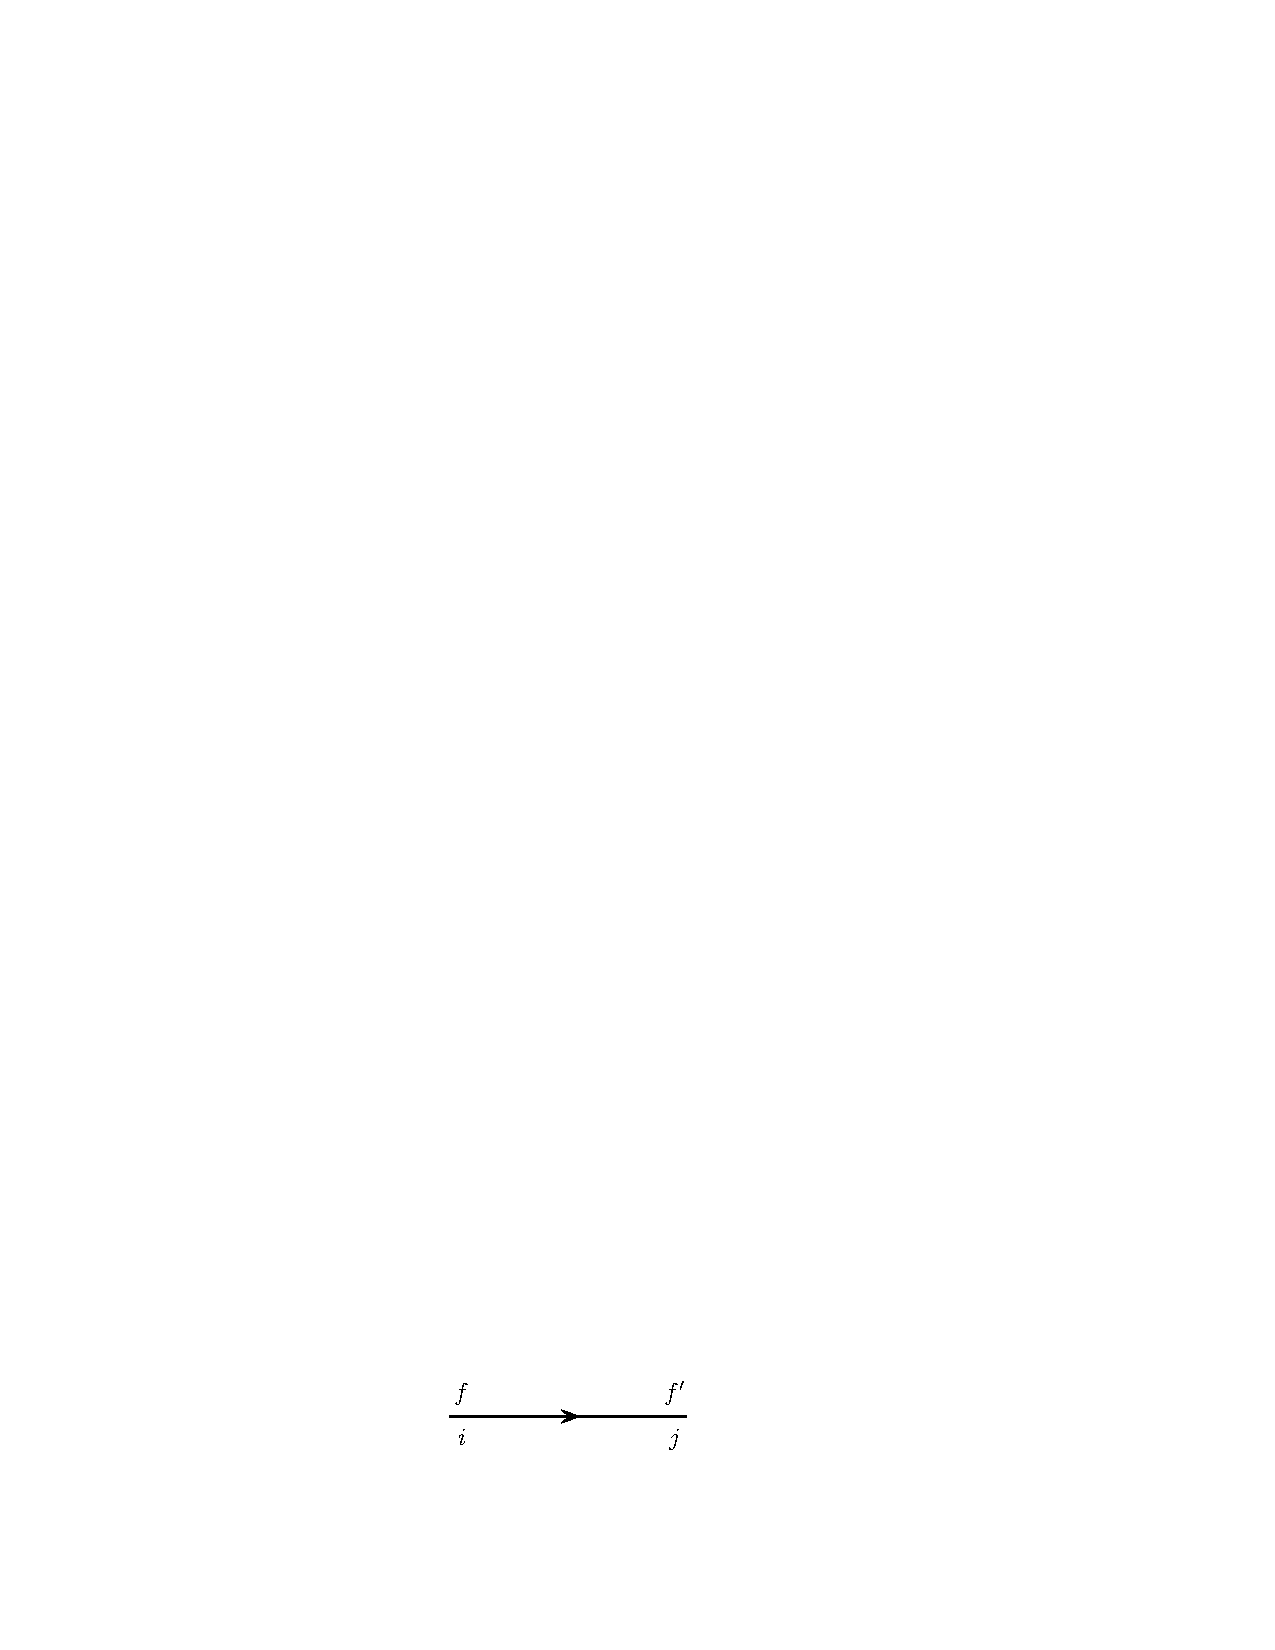
\includegraphics[width=0.5\linewidth]{quarkProp}\end{center}
				&
				\begin{center}
					\begin{equation*}
						\frac{i\delta_i^j\delta_f^{f'}(\slashed k + m)}{k^2 - m^2}
					\end{equation*}
				\end{center} \\

				\begin{center}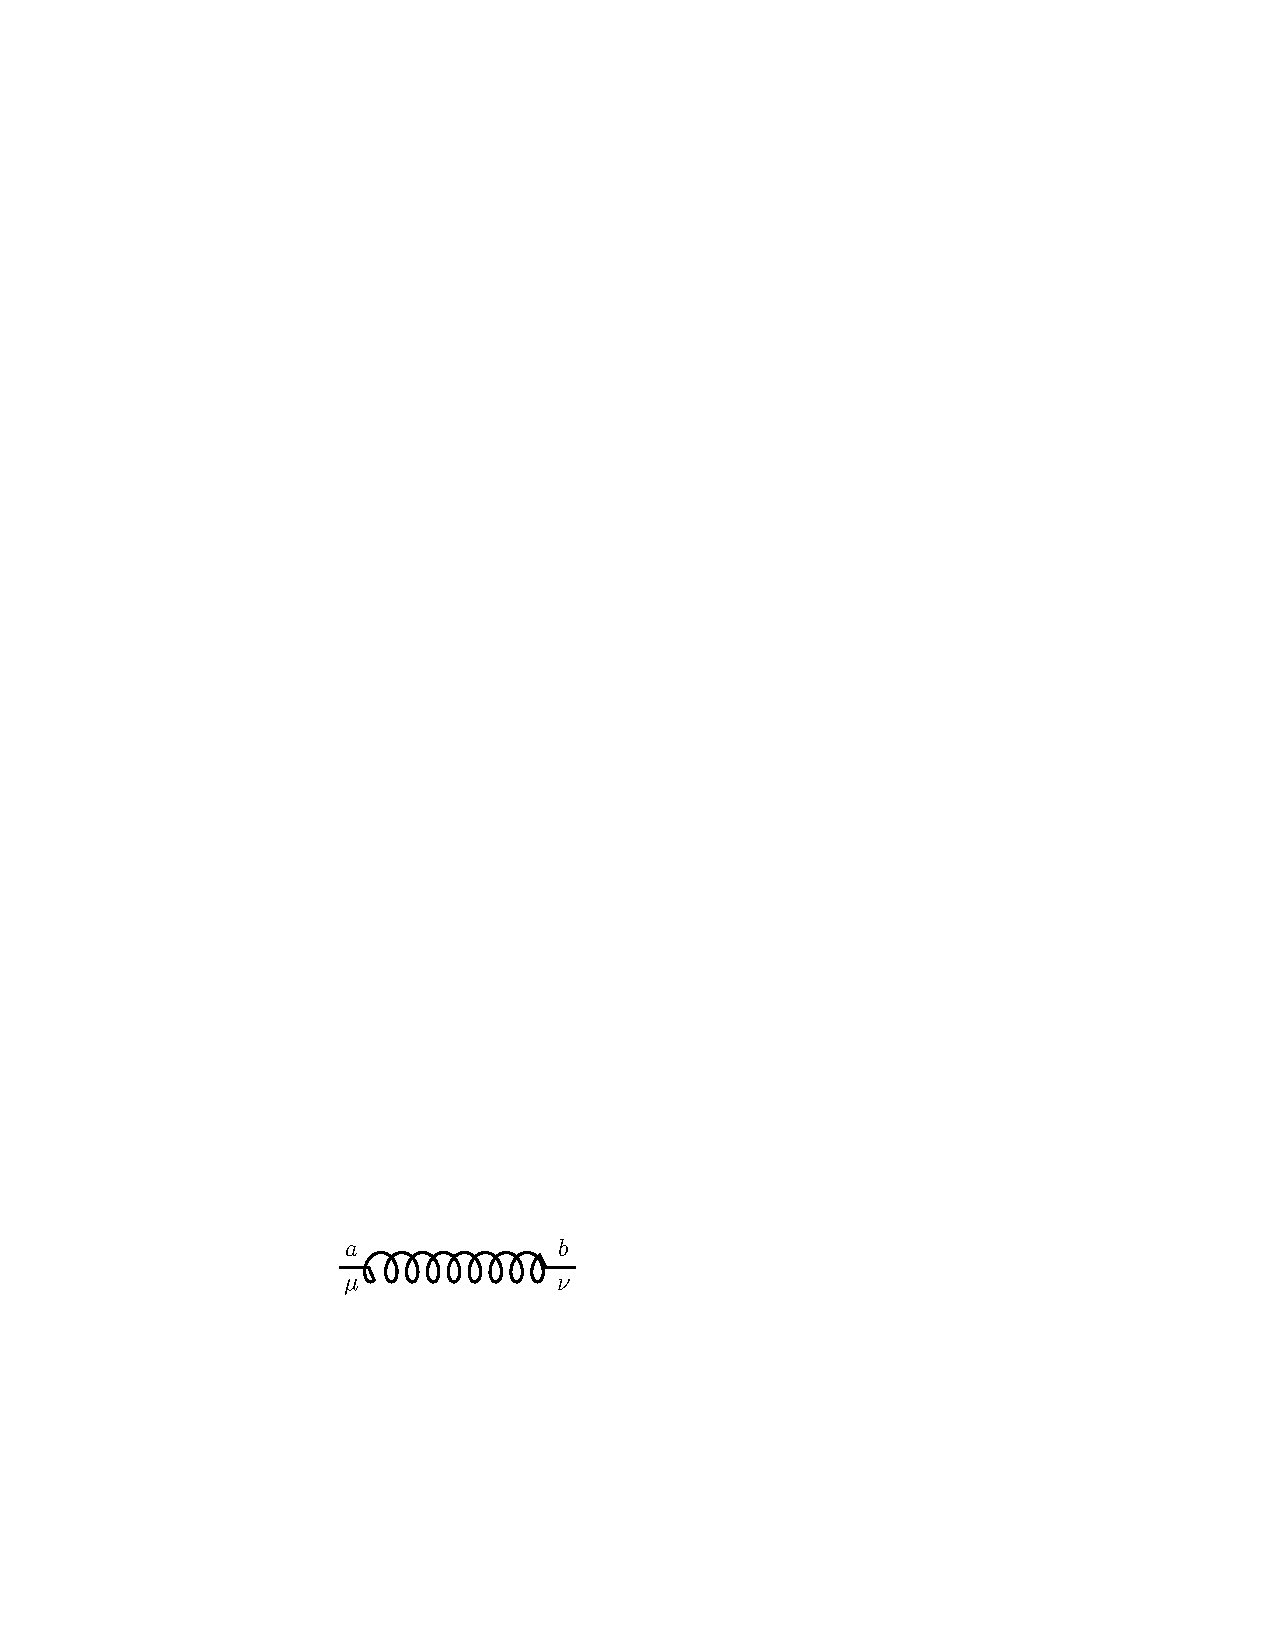
\includegraphics[width=0.5\linewidth]{gluonProp}\end{center}
				&
				\begin{center}
					\begin{equation*}
						-\frac{i\delta_a^b}{k^2}\left(g^{\mu\nu} - (\xi - 1)\frac{k^\mu k^\nu}{k^2}\right)
					\end{equation*}
				\end{center} \\

				\begin{center}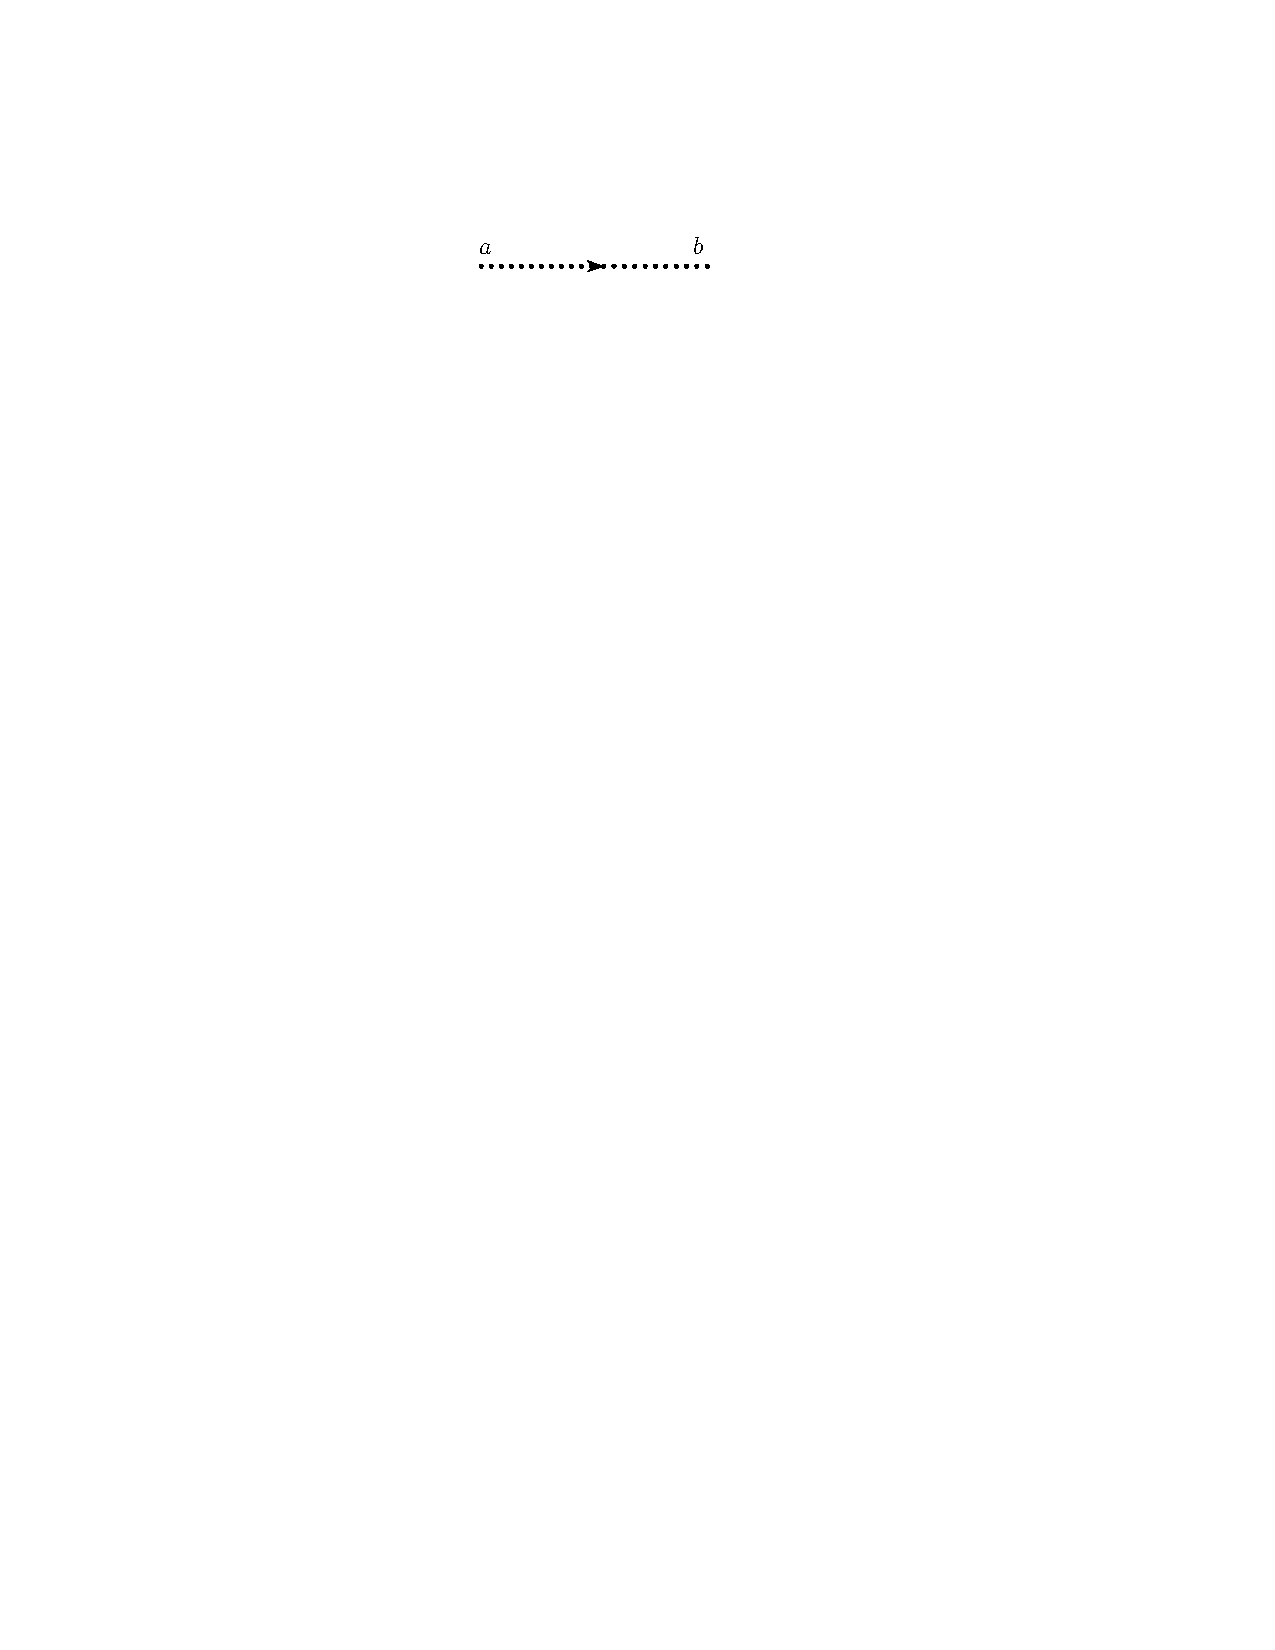
\includegraphics[width=0.5\linewidth]{ghostProp}\end{center}
				&
				\begin{center}
					\begin{equation*}
						\frac{i\delta_a^b}{k^2}
					\end{equation*}
				\end{center} \\

				\begin{center}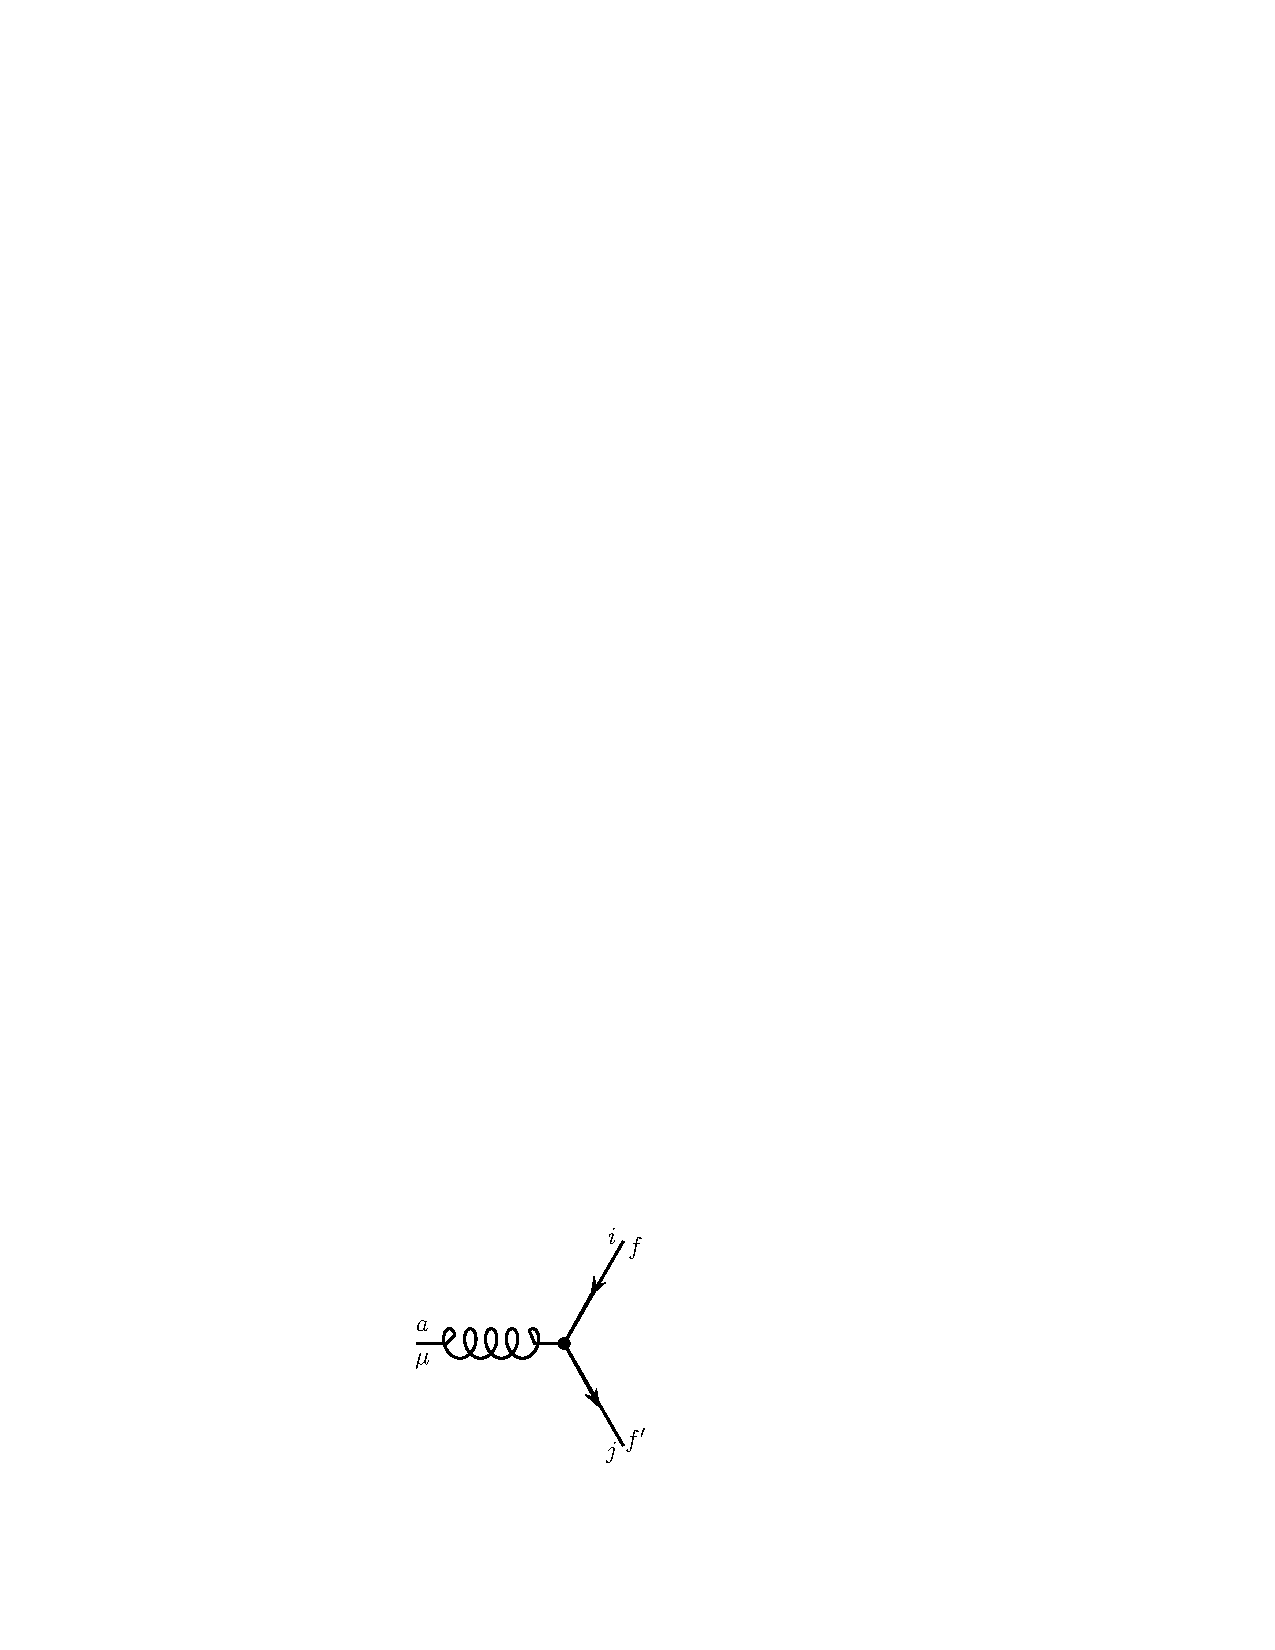
\includegraphics[width=0.40\linewidth]{qgVertex}\end{center}
				&
				\begin{center}
					\begin{equation*}
						-ig_s\gu{\mu}\delta_f^{f'}T^a_{ij}
					\end{equation*}
				\end{center} \\

				\begin{center}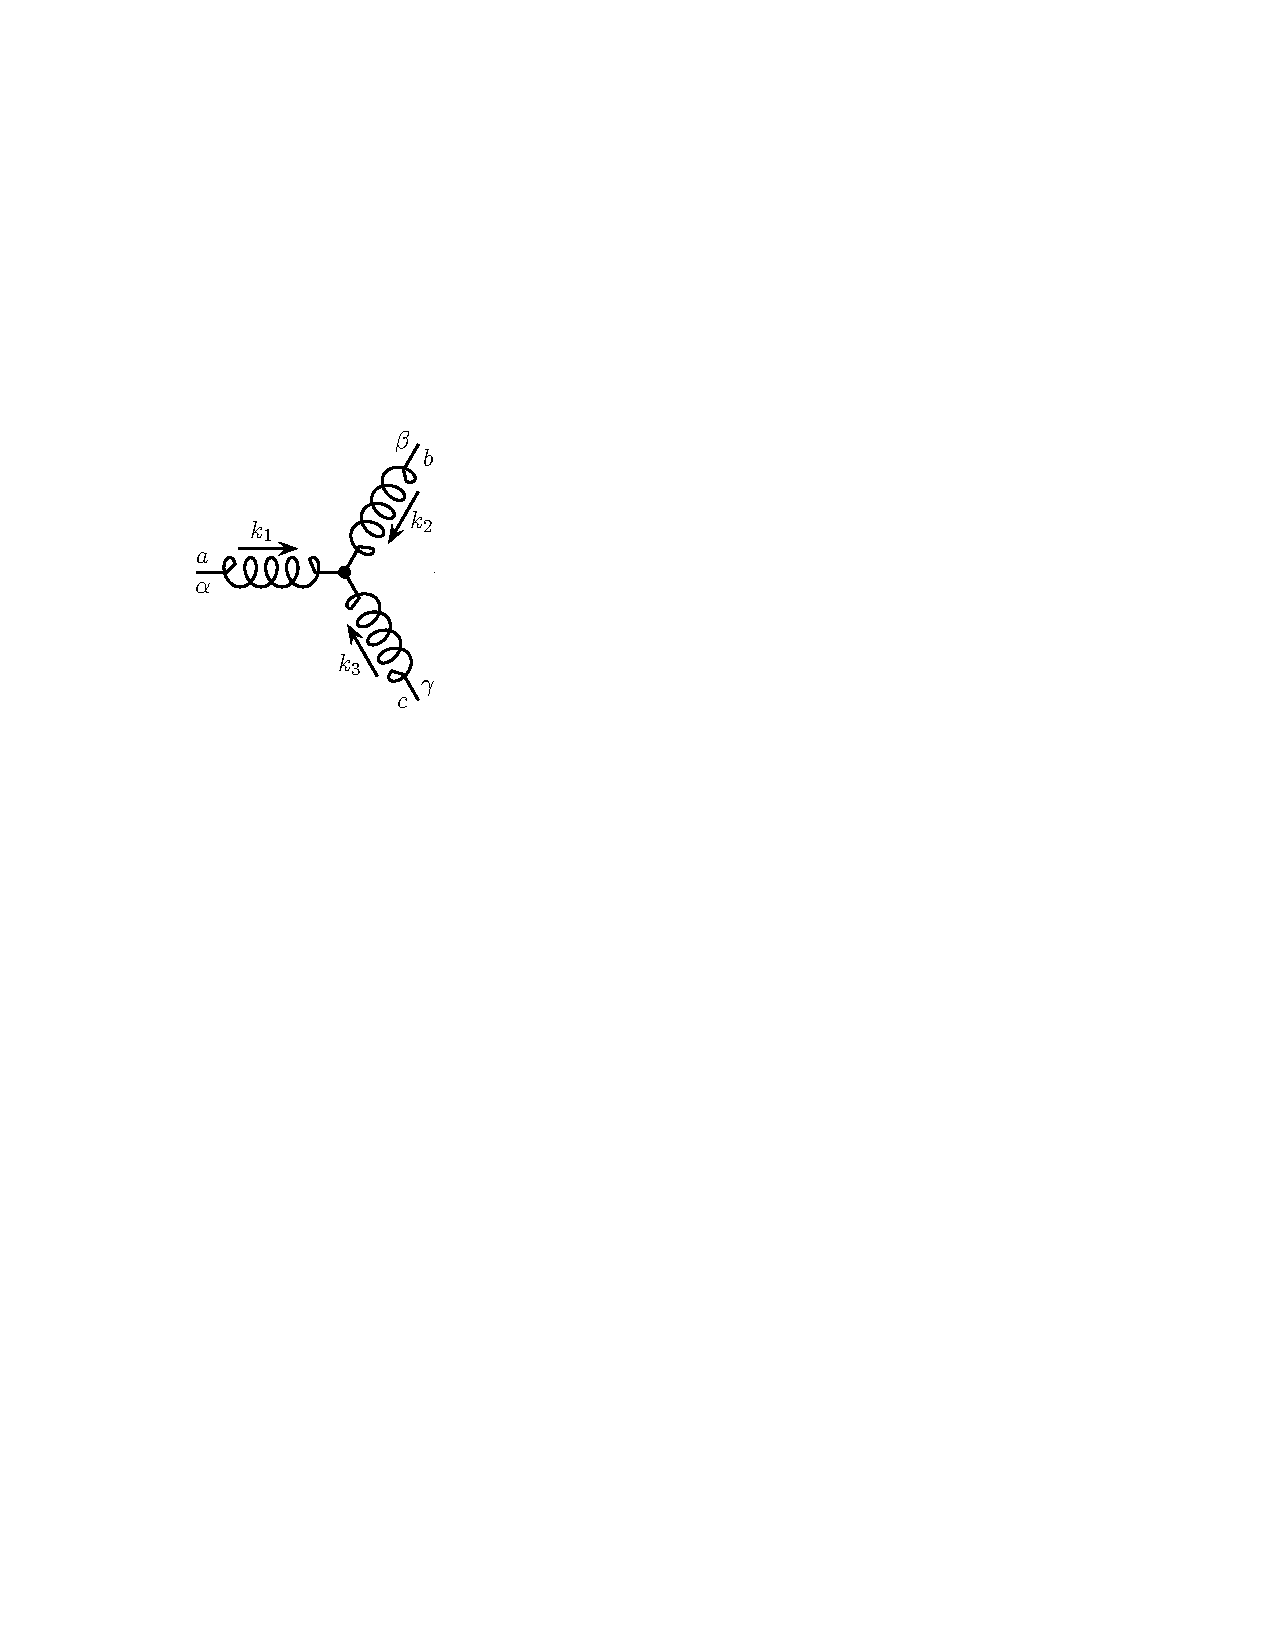
\includegraphics[width=0.40\linewidth]{tripleGluon}\end{center}
				&
				\begin{center}
					\begin{align*}
						-g_s f^{abc}\Big (g^{\alpha\beta}(k_{1} - k_{2})^{\gamma} + \\
						                  g^{\beta\gamma}(k_{2} - k_{3})^{\alpha} + \\
						                  g^{\gamma\alpha}(k_{3} - k_{1})^{\beta}\Big)
					\end{align*}
				\end{center} \\

				\begin{center}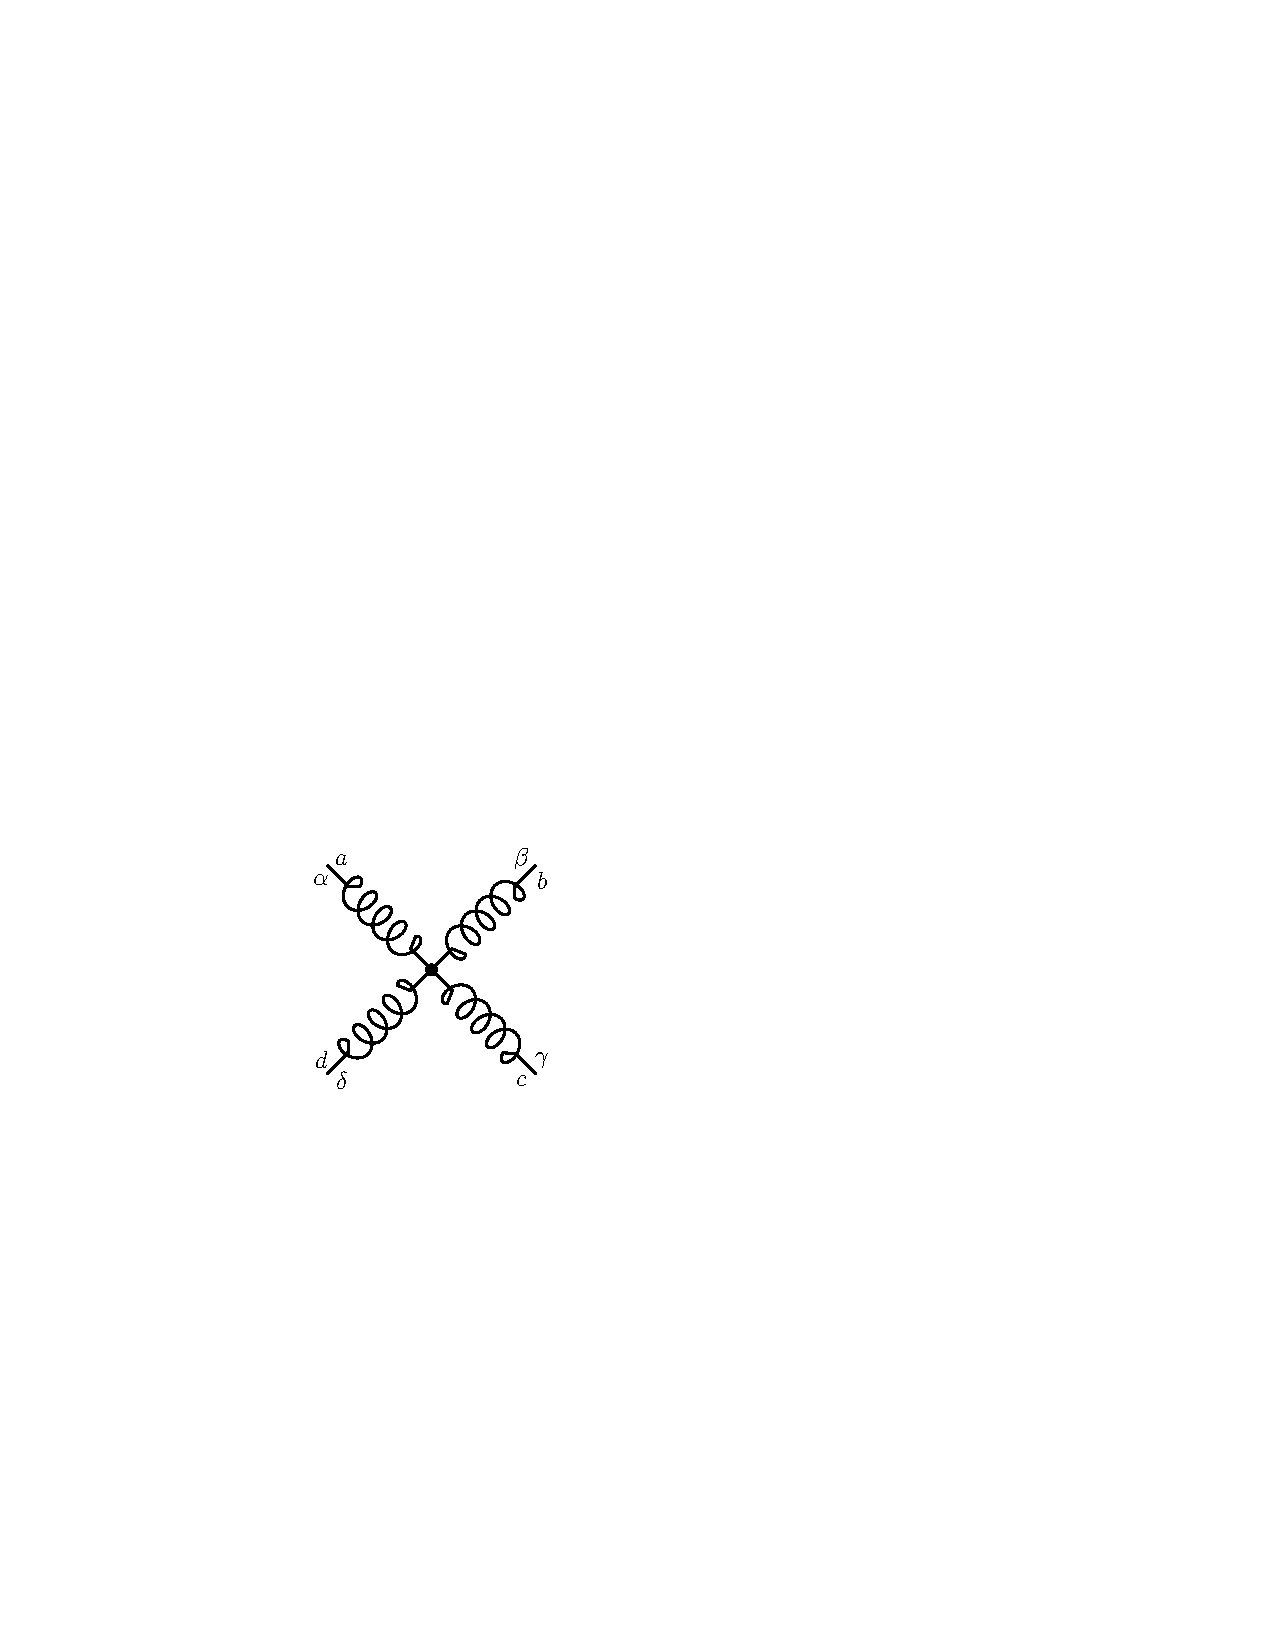
\includegraphics[width=0.40\linewidth]{quadGluon}\end{center}
				&
				\begin{center}
					\begin{align*}
						-ig_s^2\Big(f^{abe}f^{cde}(g^{\alpha\gamma}g^{\beta\delta} - g^{\alpha\delta}g^{\beta\gamma}) + \\
						            f^{ace}f^{bde}(g^{\alpha\beta}g^{\gamma\delta} - g^{\alpha\delta}g^{\gamma\beta}) +  \\
						            f^{ade}f^{bce}(g^{\alpha\beta}g^{\delta\gamma} - g^{\alpha\gamma}g^{\delta\beta})\Big) \\
					\end{align*}
				\end{center} \\

				\begin{center}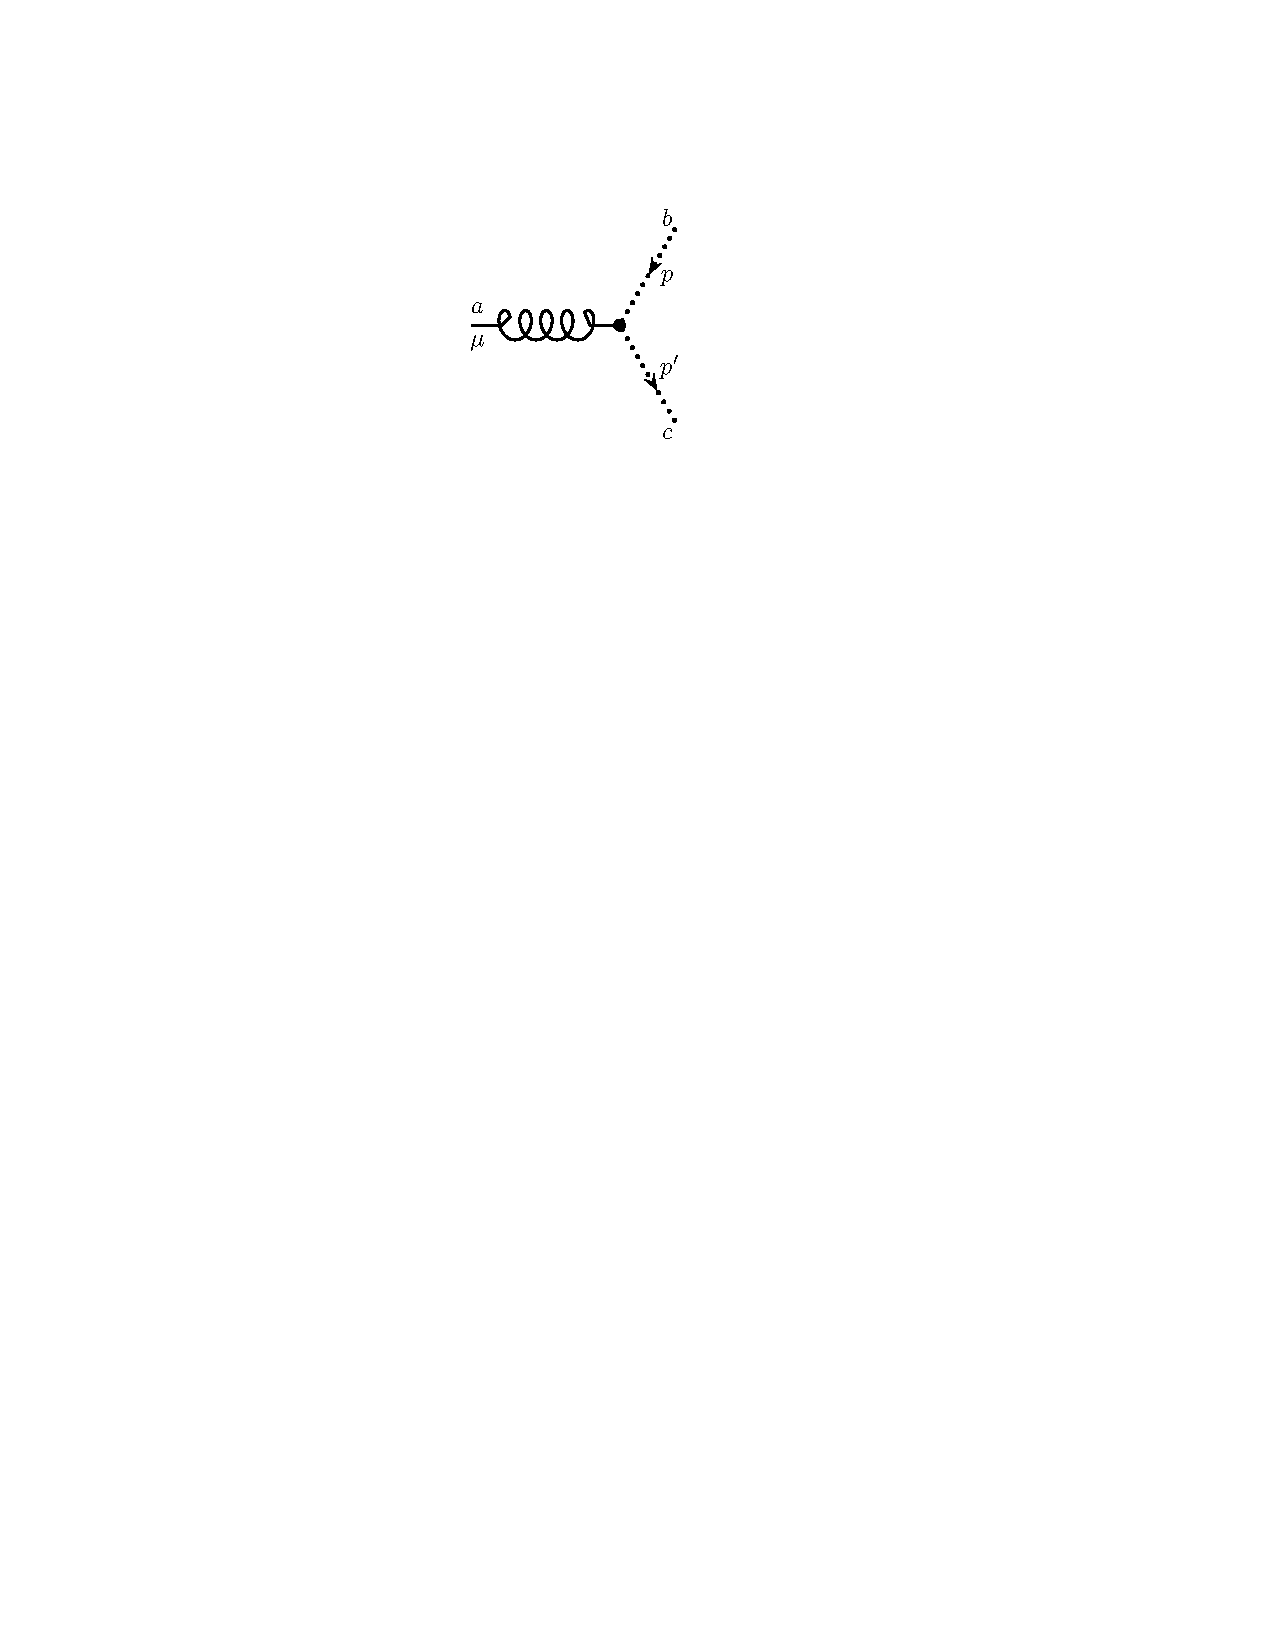
\includegraphics[width=0.40\linewidth]{gluonGhost}\end{center}
				&
				\begin{center}
					\begin{equation*}
						if^{abc}p'_{\mu}
					\end{equation*}
				\end{center} \\
			\hline
		\end{tabular}
		\label{tab:feynRules}
	\end{table}

	\begin{enumerate}
		\item Incoming external lines with spin $s$ and momentum $p$ are given a factor of $u^{(s)}_i(p)$ or
		      $\overline{v}^{(s)}_i(p)$ for quarks or anti-quarks.  Similarly outgoing external quark or
		      anti-quark lines get a factor $\overline{u}^{(s)}_i(p)$ or $v^{(s)}_i(p)$.  If the external particles
		      are not coloured the procedure is the same but of course the spinors will no longer be $SU(3)$
		      fundamental vectors.  External gluons with momentum $p$, polarisation $\epsilon$ and colour $a$ are
		      replaced by $\epsilon^a(p)$ or $\epsilon^{a*}(p)$ depending on whether they are incoming or outgoing.
		\item For each vertex or propagator in the Feynman diagram insert the corresponding mathematical
		      expression (see tab.~\eqref{tab:feynRules}).  The order of the Lorentz indices must be the same
		      as that found by tracing the fermion lines in the diagram backwards,
		\item A factor of $-1$ must be included for each anti-fermion line flowing from the initial state
		      to the final state,
		\item A factor of $-1$ must be included for each fermion, anti-fermion or ghost loop in the diagram
		\item An integration over any unconstrained momenta in the diagram must be included with measure:
		      \begin{equation}
		      	\int\frac{d^4k}{(2\pi)^4},
		      \end{equation}
		      where $k$ is the momenta in question and the integral is understood to run over all four momentum
		      components form zero up to infinity,
		\item A diagram dependent symmetry factor must be included,
		\item Lastly, for an unpolarised calculation we must sum over initial spin and colour and average
		      over all possible final spins and colours.
	\end{enumerate}

	The $u(p)$ and $v(p)$ are Dirac spinors which solve the free Dirac eq. for a plane-wave:

	\begin{equation}
		(i\slashed p - m)u(p)=0\hspace{1cm}(i\slashed p + m)v(p)=0.
		\label{eqn:diracPW}
	\end{equation}

	The result of following these Feynman rules is what we refer to as the matrix element, $\mathcal{M}$.  We will now detail how
	we go from the matrix element of some scattering process to a useful physical observable: the \emph{partonic cross-section},
	$\hat{\sigma}$.  The matrix element is related to the fully-differential cross-section by `Fermi's golden rule' which, for
	a scattering process $p_{a} + p_{b}\rightarrow p_{1} + \ldots + p_{m}$ is given by

	\begin{align}
	\begin{split}
		d\hat{\sigma} = &\frac{|\mathcal{M}(p_{a} + p_{b}\rightarrow p_{1}^{(f)}, \ldots, p_{m}^{(f)})|^2}{F}\\
		\times&(2\pi)^4\delta^{(4)}(p_{a} + p_{b} - p_{1} - \ldots - p_{m}) \\
		\times&\frac{d^3\vec{p}_1}{2E_1(2\pi)^3}\cdots\frac{d^3\vec{p}_m}{2E_m(2\pi)^3},
	\end{split}
	\end{align}

	where $F=4\sqrt{(p_ap_b)^2 - m_a^2m_b^2}$ is the flux of the incoming particles and the delta function acts to
	enforce momentum conservation for the process.\\We now have a procedure for going from a scattering process
	we wish to calculate to the differential cross-section for that process.

\section{Divergences and Regularisation}
	\label{sec:divAndReg}

	In the preceding section we saw that any unconstrained momenta in a Feynman diagram must be integrated over to account
	for all possible ways the momenta in the process may flow.  We refer to these contributions as loop-level or
	higher-order corrections.  When calculating these corrections we encounter divergences of various kinds which can be
	divided up into three classes based on how they arise.

	\subsection{Ultraviolet divergences}

		Ultraviolet divergences (UV) occur when all the components of a loop momenta grow large,
		$k^\alpha\rightarrow\infty$, such that $k^2$ becomes the dominant term in propagator.
		Since these extremely high momentum modes correspond to physics at very short distance scales
		we choose to interpret these divergences as an indication that our theory is only an na\"ive
		theory and we shouldn't attempt to apply it to all scales.  We can quickly spot diagrams with these
		pathologies with a power counting argument.  For example, given a diagram which results in a
		term such as the following:

		\begin{equation}
			\int \frac{d^4k}{k^2(k^2-m^2)},
		\end{equation}

		where $m$ is some finite mass. In the UV region where $k\rightarrow\infty$ this is asymptotically equal
		to:

		\begin{equation}
			\sim\int\frac{d^4k}{k^4},
		\end{equation}

		which is clearly logarithmically divergent.

	\subsection{Infrared and collinear divergences}

		Infrared and collinear divergences (IRC) occur in theories with massless gauge bosons, such as
		QED and QCD, since a particle may emit any number of arbitrarily such bosons with infinitesimal
		energy and we would never be able to detect their emission.  In contrast to the UV divergences
		the IR becomes important in the region of phase space where $k^2\rightarrow0$.  A similar power
		counting analysis to that above can be applied here.  For example if we consider the one-loop
		correction to the vertex diagram in massless phi-cubed from section \eqref{sec:partonicCrossSection}
		we would find an integral of the form \cite{Sterman:1995fz}:

		\begin{equation}
			I = \int\frac{d^4k}{(2\pi)^4}\frac{1}{k^2(p_1-k)^2(p_2+k)^2},
		\end{equation}

		where $k$ is the loop momentum, $q=p_1+p_2$ is the incoming momentum and $p_i$ the outgoing
		momenta.  Writing each momentum in light-cone coordinates with $p_1$ in the plus-direction,
		$p_2$ in the minus-direction, such that:

		\begin{align}
			p_1 \sim (p_1^+, 0, \vec{0}) \hspace{0.75cm} p_2 \sim (0, p_2^-, \vec{0}).
		\end{align}

		and then taking the Eikonal approximation, we have:

		\begin{align}
			I &= \int\frac{dk^+k^-k^2_T}{(2\pi)^4}\frac{1}{(2k^+k^- - k_T^2)(-2p_1^+k^-)(2p_2^-k^+)},\\
			  &= \frac{1}{2q^2}\int\frac{dk^+k^-k^2_T}{(2\pi)^4}\frac{1}{(2k^+k^- - k_T^2)(-k^-)(k^+)},
			  \label{eqn:IRCscaling}
		\end{align}

		where $q^2=2p_1\cdot p_2$ since $p_i$ are massless.  Here we can further subdivide the divergences
		into a `soft' sector and a collinear one.\\Considering first the soft regime if we
		let all the components of our integration variable, $k_\mu$ become small at the same rate, that is,
		$k^\mu\sim\lambda\sqrt{q^2}$ where $\lambda\rightarrow0$ then after a change of variables equation
		\eqref{eqn:IRCscaling} becomes:

		\begin{equation}
			I \sim\int\frac{d^4\lambda}{\lambda^4},
			\label{eqn:IRdivergent}
		\end{equation}

		which diverges logarithmically for small lambda.  The collinear sector follows similarly if we now
		look at the following scaling:

		\begin{align}
			k^\pm\sim\sqrt{q^2}\hspace{0.75cm}k^\mp\sim\lambda^2\sqrt{q^2}\hspace{0.75cm}k_T^2\sim\lambda\sqrt{q^2}.
		\end{align}

		As we decrease $\lambda$ we make $k_\mu$ increasingly collinear to either $p_1$ or $p_2$.  Using
		this scaling exactly reproduces eqn.~\eqref{eqn:IRdivergent} and therefore is also divergent.

	\subsection{Regularising divergences}
		\label{sub:regularising}


		If we are to extract any useful information from diagrams contributing above leading-order we must find
		ways to control these divergences.  These methods are called `regularisation schemes'.  The
		general plan with all regularisation schemes is to introduce a new parameter to the calculation which
		is used to get a handle on exactly \emph{how} the integral diverges.  Once we have performed the integration
		we take the limiting case where the effect of the regulator vanishes and we will see that the divergence now
		presents itself as some singular function of the regulator.  There are
		many ways to regularise divergences each with their own advantages and disadvantages.  Here we briefly describe
		three common approaches.

		Given that the integrands seen so far only diverge in certain regions (very large or very small momenta)
		perhaps the most obvious thing to do is to manually introduced alter the limits of our integration. This
		is the momentum cut-off scheme. we simply replace the upper (lower) bound with some finite large (small)
		value, $\Lambda^2$.  This will regulate any UV (soft) divergences and allow us to complete the calculation
		provided there are no collinear singularities which this approach cannot hope to regulate.  While this
		method has the advantage of being very conceptually simple it also has the serious disadvantages of
		breaking translational and gauge invariance.  Worse still is that simply limiting the integration to
		avoid the extremities has no effect on the collinear sector.

		An alternative which \emph{does} keep both gauge and translational invariance is the Pauli-Villars
		regularisation scheme \cite{RevModPhys.21.434}.  In this picture we introduce an extra field (or many extra fields
		\cite{FROLOV1993344}) which has the opposite spin-statistics and therefore has the effect of suppressing
		the very high mass region in the integrand as follows

		\begin{equation}
			\int\frac{d^4k}{(2\pi)^4}\frac{1}{p^2-m^2}\rightarrow\int\frac{d^4k}{(2\pi)^4}\left(\frac{1}{p^2-m^2} - \frac{1}{p^2-M^2}\right),
		\end{equation}

		where $M$ is the mass of the Pauli-Villars field with $m\ll M$.  However, once again this does not treat any
		problems in the IRC sectors.  \\Lastly we have dimensional regularisation.  Here we analytically continue the
		number of dimensions in our integral away from $d=4$.  We still want to be able to return to our physical four
		dimensional theory and so we choose

		\begin{equation}
			d=4-2\epsilon
		\end{equation}

		where $\epsilon$ is the regulator by which we control the divergence. Clearly then the limit
		$\epsilon\rightarrow 0$ would recover our original theory.  It is worth noting that there are many
		conventions for defining epsilons but up to signs and factors of 2 they are equivalent. Dimensional
		regularisation treats both the UV and the IRC divergences and translational and gauge invariance are
		preserved.  The disadvantage is that this modification changes the Dirac algebra relations which
		typically makes computing the integrals more involved.\\When working in $d$ dimensions the QCD coupling
		is no longer dimensionless.  We can see this since the action is dimensionless and therefore we have

		\begin{equation}
			[\mathcal{L}] = d.
		\end{equation}

		By considering the kinetic terms of the gluon and quark fields we can see that we must have

		\begin{equation}
			[g] + 2[\psi] + [A_\mu] = d,
		\end{equation}

		and therefore

		\begin{equation}
			[g] = \frac{4-d}{2}.
		\end{equation}

		In order to artificially fix this and restore the coupling to its dimensionless state we
		introduce a scale parameter, $\mu_r$, as follows:

		\begin{equation}
			g = g_0{\mu_r}^{\frac{4-d}{2}}.
		\end{equation}

		The introduction of this scale has important consequences for our theory.  Here we follow the instructive example
		from \cite{pinkBook}.  If we have some dimensionless observable, $R$, which depends on one large scale, $Q$, which
		is much larger than all other scales in the problem (e.g. the quark masses).  One would assume that $R$ is
		approximately independent of this large scale but when we come to regulate and renormalise the divergences we have
		seen in this section the problem becomes one involving two scales and $R$ develops a dependence on the ratio of
		these scales, $\frac{Q^2}{\mu_r^2}$.  Since $\mu_r$ is completely arbitrary $R$ must be independent of it i.e if we
		now consider $R$ as a function of both the QCD coupling strength, $\alpha_s$, and the ratio of the scales we must
		have that

		\begin{equation}
			\mu_r^2\frac{\partial R}{\partial\mu_r^2} + \mu_r^2\frac{\partial \alpha_s}{\partial \mu_r^2}\frac{\partial R}{\partial\alpha_s} = 0,
			\label{eqn:chainRuleOnR}
		\end{equation}

		for convenience we define $t = \ln\frac{Q^2}{\mu_r^2}$ and $\beta(\alpha_s) = \mu_r^2\frac{\partial \alpha_s}{\partial \mu_r^2}$
		and so we can write\eqref{eqn:chainRuleOnR} as

		\begin{equation}
			\frac{\partial R(e^t, \alpha_s)}{\partial t} - \beta(\alpha_s)\frac{\partial R(e^t, \alpha_s)}{\partial \alpha_s} = 0.
		\end{equation}

		This can be solved by defining the `running QCD coupling', $\alpha=\alpha(Q^2)$

		\begin{equation}
			t = \int_{\alpha_s}^{\alpha(Q^2)}\frac{dx}{\beta(x)},
			\label{eqn:solvingRunning}
		\end{equation}

		where $\alpha=\alpha(Q^2)$ admits the boundary condition $\alpha(\mu_r^2)=\alpha_s$.  Therefore the scale dependence
		of our observable $R$ comes about through its dependence on $\alpha_s$ only.

\section{The QCD Beta Function}
	\label{sec:betaFunction}

	QCD has two striking features which are not apparent from the Lagrangian derived above.  The first is asymptotic freedom.
	This is the fact that at \emph{high} energies the QCD coupling strength becomes increasingly weak and it is this which allows us to
	perform a perturbative expansion of physical observables such as cross-sections.  The second feature is confinement.  Confinement
	is the reason we do not observe bare quarks and gluons in nature, instead we only see bound states of these fundamental QCD partons.
	This is because at very \emph{low} energies the coupling strength becomes increasingly strong.\\As we saw in section \ref{sec:divAndReg}
	when we renormalise QCD to remove the ultraviolet singularities we introduce a scale dependence in the coupling strength,
	$\alpha_s = \alpha_s(\mu_r)$.  It can be interpreted as a measure of our ignorance of the true high-scale theory which governs nature,
	that is to say, we believe QCD is the right theory \emph{only up to} some scale $\mu_r$.  The evolution of $\alpha_s$ with $\mu_r$ is
	given by the renormalisation group equation:

	\begin{equation}
		\mu_r^2\frac{\partial\alpha_s}{\partial \mu_r^2} = \beta(\alpha_s(\mu_r^2)),
		\label{eqn:RSFlow}
	\end{equation}

	where $\beta(\alpha_s)$ is the beta function.  It can be expanded perturbatively as a series in $\alpha_s$
	as follows:

	\begin{equation}
		\beta(\alpha_s) = -\beta_0\alpha_s\left(1 + \beta_1\alpha_s + \beta_2\alpha_s^2 + \ldots \right),
		\label{eqn:betaFunction}
	\end{equation}

	where the perturbative coefficients, $\beta_i$, can be calculated using the methods of section (\eqref{sec:partonicCrossSection}.
	For example the leading order contribution, $\beta_0$, is given by:

	\begin{equation}
		\beta_0 = 11 - \frac{2n_f}{3}.
	\end{equation}

	If we truncate eq. \eqref{eqn:betaFunction} at leading-order in $\alpha_s$ then we can solve eq. \eqref{eqn:RSFlow}
	and we see that the coupling, $\alpha_s(\mu_r)$, `runs' with the following form:

	\begin{equation}
		\alpha_s(Q^2) = \frac{\alpha_s(\mu_r^2)}{1 + \alpha(\mu_r^2)\frac{\beta_0}{4\pi}\ln\frac{Q^2}{\mu_r^2}}.
		\label{eqn:runningAS}
	\end{equation}

	It is clear from this (since in the standard model we have $n_f\leq6$ and therefore $\beta_0>0$\footnote{The number of
	fermions we consider depends on the energy scale we are at. Clearly we must be at an energy larger than the mass of any
	given quark for it to be produced.  This was experimentally observed in the famous $R$-ratio where the ratio of the
	$e^+e^-\rightarrow \text{hadrons}$ cross-section to the $e^+e^-\rightarrow\mu^+\mu^-$ cross-section was investigated})
	that as $Q^2$ tends to zero the coupling strength becomes very large and at high values for $Q^2$ we see that $\alpha_s(Q^2)\rightarrow0$.
	This later limit is exactly the asymptotic freedom property of QCD and it holds even when we include the higher order
	terms we neglected in the leading-order approximation used to arrive at eq. \eqref{eqn:runningAS} \cite{Beringer:1900zz}.
	It is an essential result in that it allows us to perform perturbative expansions of observables and without this none of the
	following work would be possible.  The evolution of the strong coupling with $Q^2$ is shown in fig.~\eqref{fig:runningAS},
	it shows several extracted values of $\alpha_s$ based on six various types of experiment.  For example, the hadronic
	collider predictions include studies of the ratio of the 3-jet inclusive cross-section to the 2-jet inclusive
	cross-section as a means of finding the strong coupling \cite{Chatrchyan:2013txa}.

	\begin{figure}[htp]
		\centering
		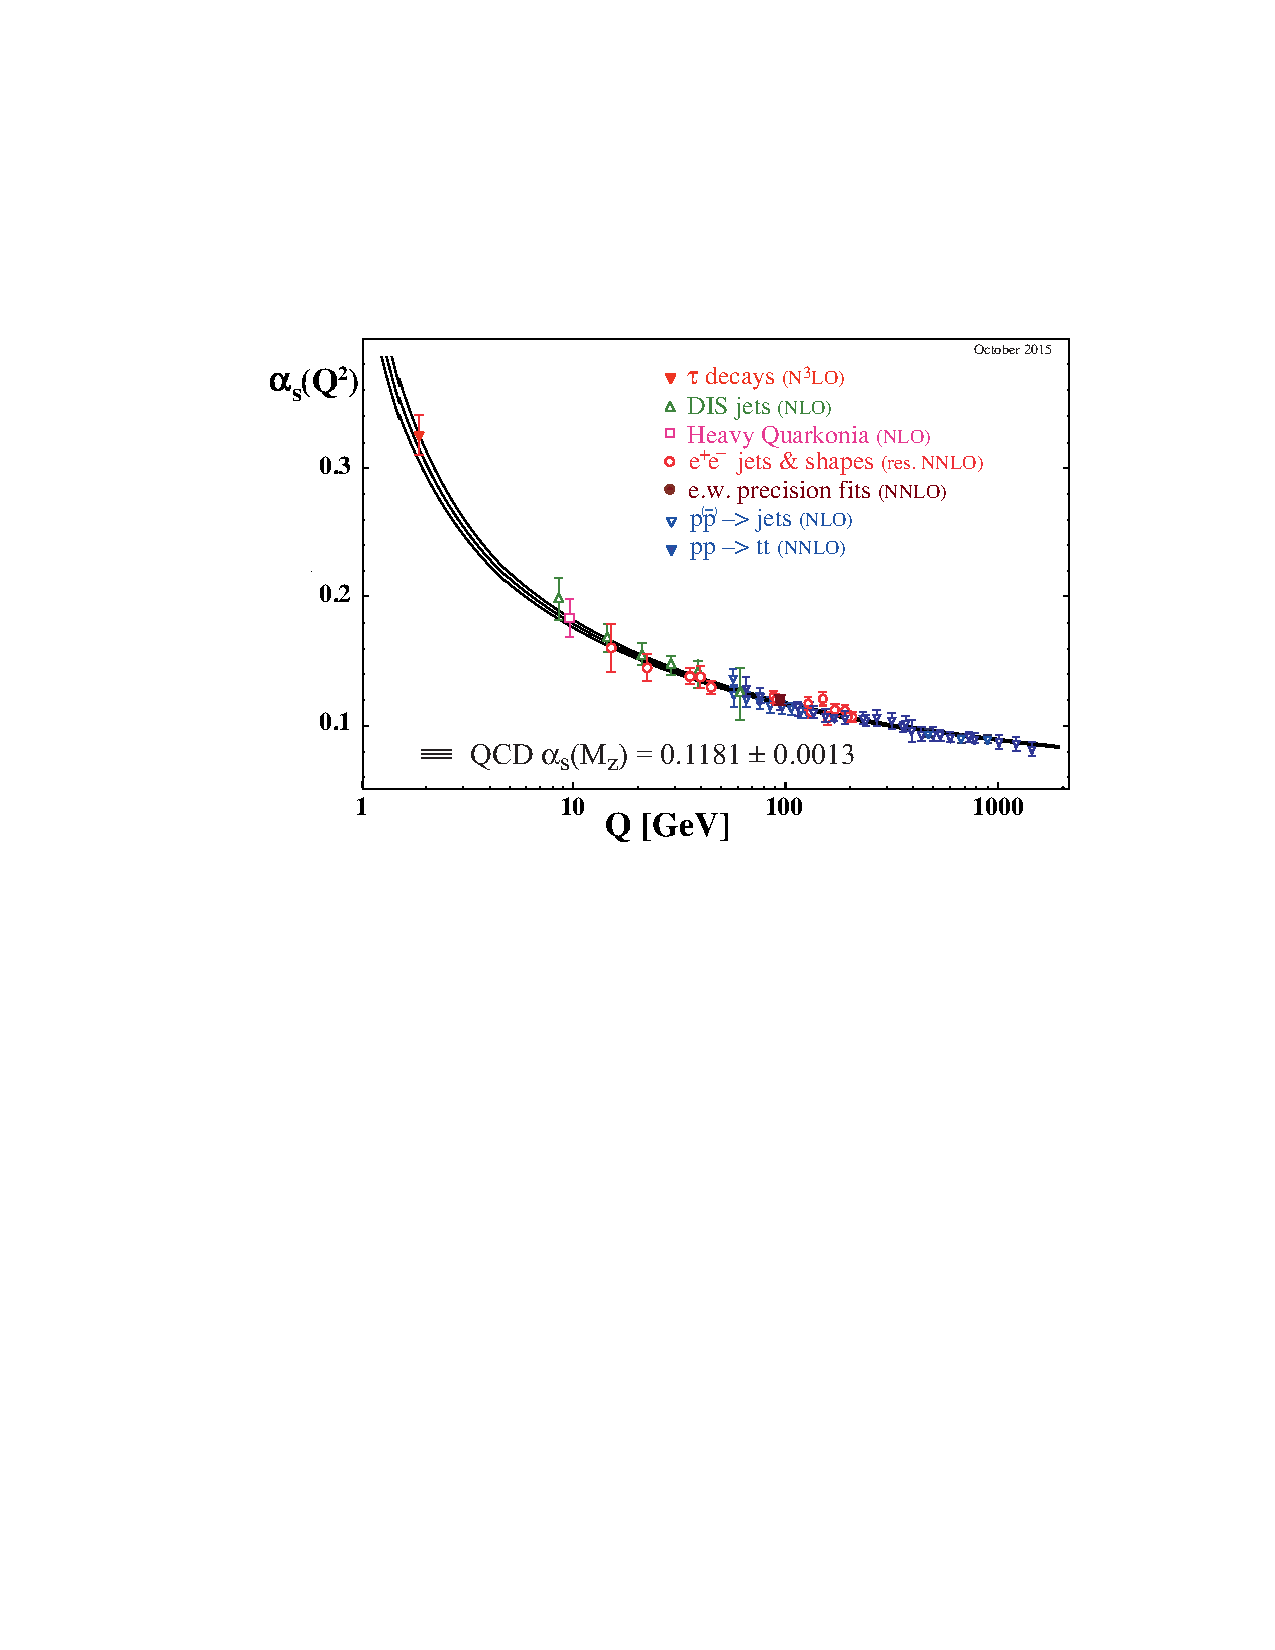
\includegraphics[width=0.9\textwidth]{Figures/runningAlphaS}
		\caption{The evolution of $\alpha_s$ over several orders of magnitude in the scale of the process $Q^2$.  The data
		         points fitted are of varying degrees of formal accuracy ranging from next-to-leading order in $\alpha_s$
		         (NLO) to next-to-next-to-next-to-leading order in $\alpha_s$ (N\textsuperscript{3}LO).
		         Fig. from \cite{Beringer:1900zz}.}
		\label{fig:runningAS}
  	\end{figure}

\section{QCD Factorisation at Hadronic Colliders}
	\label{sec:factorisation}

	So far we have only talked about the very general idea of two particles interacting and scattering off one another into
	some final state which we are interested in.  This is too simple a picture when we are considering hadronic colliders
	such as the Large Hadron Collider (proton-proton), the Tevatron (proton-antiproton), HERA (proton-lepton) and, potentially,
	a Future Circular Collider (FCC) with a hadronic initial state.\\At experiments we collide QCD bound states with one another
	but in practice when calculating cross-sections we perform a sum over the possible combinations of initial states we may
	encounter in the two incoming hadrons.  In order to do this we must have a good understanding of the dynamics of the partons
	inside the onrushing hadrons; this understanding is encoded in the Parton Distribution Functions (PDFs).  A PDF,
	$f_{i/H}(x, Q^2)$ is a function which tells us how likely we are to find a parton of type $i$ carrying a fraction $x$ of the
	total hadron's momentum in a hadron, of type $H$, during a collision occurring at an energy scale $Q$.  Because the PDFs contain
	non-perturbative information we cannot compute their properties in the same way as we calculate cross-sections, instead they
	are determined by fitting to data from a range of experiments (such as those mentioned above).  Once we have the
	PDFs we can compute the physical hadronic cross-sections, $\sigma$, by convoluting two of them (one for each hadron) with
	the partonic cross-section for the scattering of partons of type $i$ and $j$, $\hat{\sigma}_{ij}$, discussed in section
	(\ref{sec:partonicCrossSection}) and summing over the possible initial partons as follows:

	\begin{equation}
		\sigma(Q^2) = \sum_{f_a,f_b}\int_0^1dx_adx_bf_{a/H_a}(x_a, Q^2)f_{b/H_b}(x_b, Q^2)\hat{\sigma}_{ij}(\alpha_s(\mu_r), \mu_r^2, \mu_f^2).
		\label{eqn:factorisation}
	\end{equation}

	Eq. \eqref{eqn:factorisation} can be intuitively understood as a separation of scales; the long distance physics of the PDFs is
	manifestly distinct from the short distance hard scatter contained in the partonic cross-section.  The scale at which we separate the
	long and short range physics is called the \emph{factorisation scale}, $\mu_f$.  As with the renormalisation scale it is not
	\emph{a priori} clear what is the correct factorisation scale and results of perturbative calculations are often quoted with
	a `scale uncertainty' band.

\section{From Partons to Jets}

	As alluded to in section (\ref{sec:betaFunction}) the computation of scattering amplitudes can only take us so far
	when comparing simulations to experiments.  In particular, the final state quarks and gluons in our perturbative
	picture of QCD differ from the confined hadrons observed at hadronic colliders:  It is well known that final state
	QCD partons fragment and emit showers of additional radiation before finally they becomes colourless bound states
	in a process known as `hadronisation'.  This process is not perturbatively well-understood since it occurs at scale,
	often called $\Lambda_{\text{QCD}}$, at which QCD becomes non-perturbative, \emph{i.e.} the coupling constant of the
	theory has become too large for us to legitimately truncate a perturbative expansion.  There are models for both
	the `parton shower' behaviour of the energetic final state partons, such as \texttt{Pythia} \cite{Sjostrand:2007gs},
	\texttt{Herwig} \cite{Corcella:2000bw} and \texttt{Sherpa} \cite{Hoche:2014kca} as well as models for the hadronisation
	such as the `Lund string model' \cite{Andersson:2002ap} implemented in various physics software packages but most
	relevantly (for the remainder of this thesis) - in the \texttt{Ariadne} code \cite{Lonnblad:1992tz,Andersen:2011zd}.\\
	All high energy collider experiments
	see a great deal of QCD radiation in the final state.  This radiation, produced through the mechanisms outlined above,
	appears in columnated structures called `jets' and so it is at the jet level that we may compare our simulated results
	to actual measurements. The question of how we best map from the two or more parton level to the jet level is not a trivial
	one:  a single high-energy (or `hard') parton may split and form two final state jets but equally two low energy (or
	`soft') partons may combine into a single jet.\\There are several approaches to this problem include the \texttt{SISCone}
	algorithm \cite{Salam:2007xv} and Pythia's own implementation \texttt{CellJet} \cite{Sjostrand:2000wi}. However the
	most commonly user family of jet reconstruction algorithm are know as the `sequential recombination algorithms'.
	This group of approaches include the Cambridge-Aachen, $k_T$ and anti-$k_T$ algorithms. The general algorithm, as
	given in \cite{Cacciari:2008gp}, is:

	\begin{enumerate}
		\item Given a list of final state partons calculate some generalised distance, $d_{ij}$, between all possible
		      combinations of jets $i$ and $j$ as well as $d_{iB}$ where $B$ is the beam-line,
		\item We identify the smallest value of these.  If, say $d_{ab}$ is the smallest, we combine partons $a$ and $b$.
		      If however $d_{aB}$ is the smallest then we call $a$ a jet and remove it from the list of partons,
		\item We then recompute all the generalised distances and repeat steps 1 and 2 until no further partons remain,
	\end{enumerate}

	where the generalised distances are defined as

	\begin{align}
	\begin{split}
		d_{ij} &= \text{min}(k_{Ti}^{2p}, k_{Tj}^{2p})\frac{\Delta R^2}{R^2},\\
		d_{iB} &= k_{Ti}^{2p},
	\end{split}
	\end{align}

	where $k_{Ti}$ is the transverse momentum of the $i^{th}$ parton, $R$ is a free parameter in the clustering which relates
	to the size of the jets and $\Delta R^2$ is the distance in the detector metric between the two partons given by
	$\Delta R^2 = \Delta\phi^2 + \Delta y^2$ where $\Delta\phi$ and $\Delta y$ are the angular distance (about the beam line)
	between the partons and the rapidity gap between the partons respectively.  The parameter is $p$ and it is this which
	specifies precisely which clustering algorithm we are using; $p=0$ reduces to the Cambridge-Aachen scheme while
	$p=\pm1$ give the $k_T$ and anti-$k_T$ respectively.  The question of which to use is outlined in detail in
	\cite{Cacciari:2008gp} but we give a brief summary here.\\The choice of jet algorithm boils down to a handful of key
	properties the algorithm must exhibit.  Given a set of hard QCD final states we require that the result of the
	clustering algorithm, i.e. the jets and jet shapes, are not unduly sensitive to additional soft and collinear radiation.
	This is intuitively clear since, for example, a final state with a single high energy quark with momentum, $k_{Ti}$,
	may radiate infinitely a multitude of infinitely soft gluons, $k_{Ts_i}$, which may (or may not) be collinear to the
	original parton - but since $k_{Ts_i}\ll k_{Ti}$ the result must be a single jet, $j_{Ti}$, which has $j_{Ti}\sim k_{Ti}$.
	Any algorithm which satisfies this is said to be infra-red and collinear (IRC) safe.  We also want an algorithm which
	is insensitive to the hadronisation model used, or any possible extra multiple-parton or experimental pile-up emissions
	since these things are, at present, poorly understood.  It is also worth mentioning that since jet clustering algorithms
	are used in experimental triggers to quickly catagorise events they should be as computationally cheap as possible.\\Although
	the Cambridge-Aachen algorithm has advantages in some experimental searches such as studies where the substructure of
	jets is of particular interest \cite{Butterworth:2008iy, Aad:2015owa}, the most widely used sequential recombination algorithm is
	the anti-$k_t$ algorithm ($p=-1$) and so all of the work which follows and all of the experimental comparisons made will
	use this as the method for mapping simulated parton level results to a more useful set of jet level results.  The jet size
	parameter $R$ varies between experiments but is typically either 0.4 for ATLAS analyses or 0.5 for CMS analyses.

\section{Perturbative QCD and Resummation}
	\label{sec:pqcdAndResum}

	In section \ref{sec:partonicCrossSection} we saw that we could separate out the QCD Lagrangian into
	free and interacting components and that vacuum expectations of time ordered fields could be found by
	taking functional derivatives of the free partition function (eqn.~\eqref{eqn:fnDerviatesOfLagrangian}).
	Since terms which give rise to interactions in the Lagrangian come with a factor of the coupling strength,
	$g$, Taylor expanding the exponential in eqn.~\eqref{eqn:fnDerviatesOfLagrangian} will yield an infinite
	series of terms and, in principle, in order to compute any physical observable we must calculate we must
	evaluate all of these.  Of course in practice this is not possible.  We must choose a subset of terms from
	this infinite array which we reason will give the \emph{best possible approximation to the full series}.

	\subsection{Fixed-order Perturbation}

		The fixed-order perturbative approach operates on the assumption that since, as we saw in section \ref{sec:betaFunction},
		the coupling strength $\alpha_s$ in the expansion becomes small at large energy scales we may truncate the series at some
		power of $\alpha_s$.  For example given a cross-section of a scattering $X\rightarrow Y$ we wish to calculate, the fixed
		order picture of the expansion would be:

		\begin{equation}
			\sigma_{X\rightarrow Y} = \alpha_s^{i_0}(Q^2)\sum_{i=1}^N\alpha_s^{i}(Q^2)\mathcal{C}^{(i)}_{X\rightarrow Y}
		\end{equation}

		where $i_0$ accounts for processes which start above tree level and $\mathcal{C}^{(i)}_{X\rightarrow Y}$
		are the coefficient terms which encode the kinematics of the diagrams contributing at each `order'
		in the series.  Since we expect that the more terms we can calculate the better our
		truncated series will approximate the full result we should choose $N$ as large as possible though in principal
		it is determined by the complexity and the computational cost of the relevant calculation of the coefficient
		functions.  Recent progress has allowed the automation of next-to-leading order QCD calculations ($N=2$) in
		packages such in \texttt{aMC@NLO\_MadGraph} (v5) \cite{Alwall:2011uj}, \texttt{BlackHat} \cite{Bern:2012my}, \texttt{MC@NLO}
		\cite{Frixione:2010wd} and \texttt{Powheg} \cite{Frixione:2007vw}.  In general it is not known how to compute
		multi-loop (i.e. $N\geq3$) calculations and while process specific calculations have been completed
		\cite{Cacciari:2015jma, Grazzini:2015nwa, Gehrmann:2014fva}, it is still very much a hot topic in theoretical
		physics.\\It is important to note the limitations of this fixed-order scheme.  For example, if we were to consider
		NLO corrections to dijet production we would only be able to produce final states with two or three jets (since
		we can only have one extra real emission).  Clearly this is a limitation since the external fermion lines can
		radiate arbitrarily many extra gluons.  It is precisely this phenomenon which is shown in fig. 9,
		the NLO calculations (shown in green and black) are limited to $\langle jets\rangle\leq3$ which the predictions
		from \texttt{POWHEJ+PYTHIA} and \texttt{HEJ} which include higher-order corrections predict a higher average
		number of jets.  Note that the higher-order corrections here are \emph{not} the same in the case of
		\texttt{POWHEJ+PYTHIA} and \texttt{HEJ}.  Also note that although the scale uncertainty band of the NLO
		calculation \emph{does} exceed $\langle jets\rangle=3$ this is not a result of the formalism but instead comes
		about as the result of an attempt to quantify the residual dependence of the calculation on the factorisation
		and renormalisation scales.  This scale dependence of observables will be discussed in more detail in chapter
		\ref{chap:Zs}.\\There are frameworks to allow the `merging' of NLO calculations of different multiplicity.  A
		comprehensive review of such methods may be found in \cite{Alwall:2007fs}.

		We now present an instructive fixed-order calculation of the next-to-leading corrections to quark-antiquark pair
		production via an off-shell photon \cite{fieldBook}.

		\begin{figure}[hbt]
			\centering
			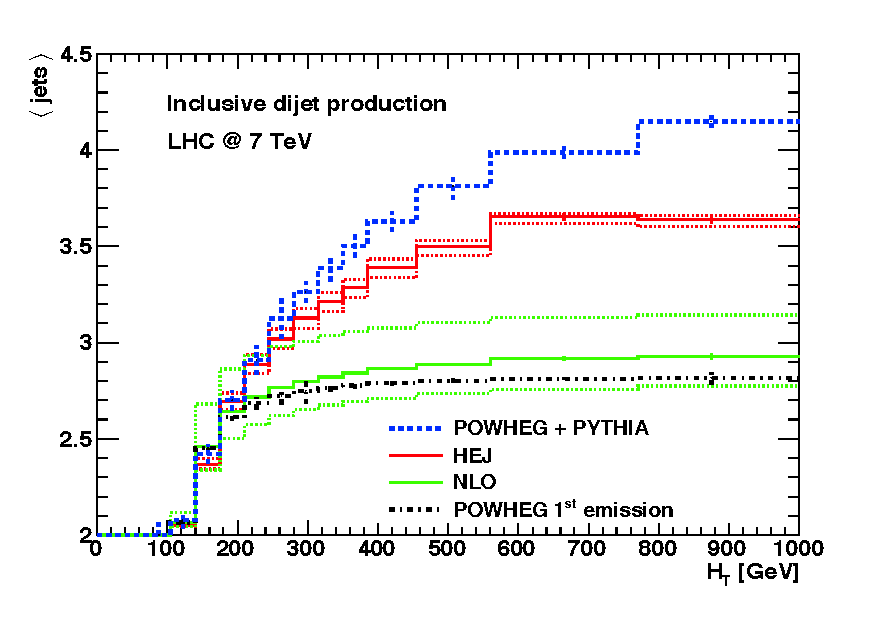
\includegraphics[width=\textwidth]{NLOfail}
			\caption{Simulations of the average number of jets as a function of the sum of the transverse momenta in the event, $H_T$,
			         for inclusive dijets at a 7TeV LHC.}
			\label{fig:NLO3jets}
  		\end{figure}

	\subsection{An Example Fixed-Order Calculation}
		\label{sub:eg1loop}

		\begin{figure}[tpb]

			\centering

			\begin{subfigure}[b]{0.48\textwidth}
				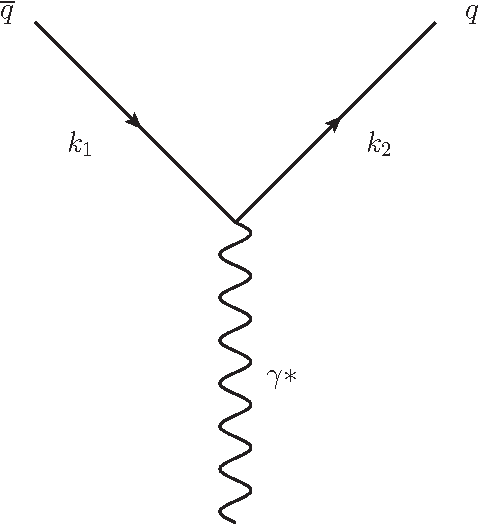
\includegraphics[width=0.8\textwidth]{TreeLevel}
				\caption{$\mathcal{A}_0$}
				\label{fig:NLOfig_1}
			\end{subfigure}
			\begin{subfigure}[b]{0.48\textwidth}
				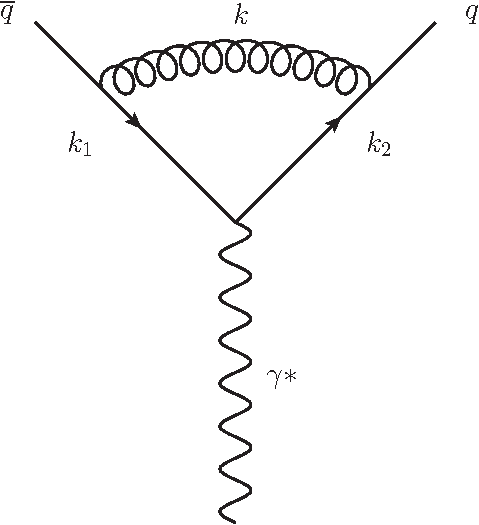
\includegraphics[width=0.8\textwidth]{NLOVirtual}
				\caption{$\mathcal{A}_v$}
				\label{fig:NLOfig_2}
			\end{subfigure}
			\begin{subfigure}[b]{0.48\textwidth}
				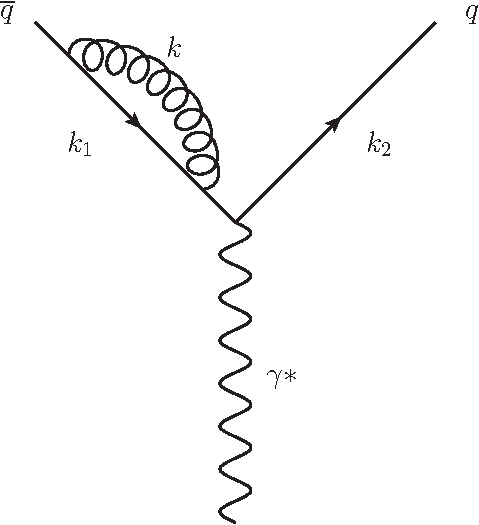
\includegraphics[width=0.8\textwidth]{NLOSelfEnergyLeft}
				\caption{$\mathcal{A}_{se1}$}
				\label{fig:NLOfig_3}
			\end{subfigure}
			\begin{subfigure}[b]{0.48\textwidth}
				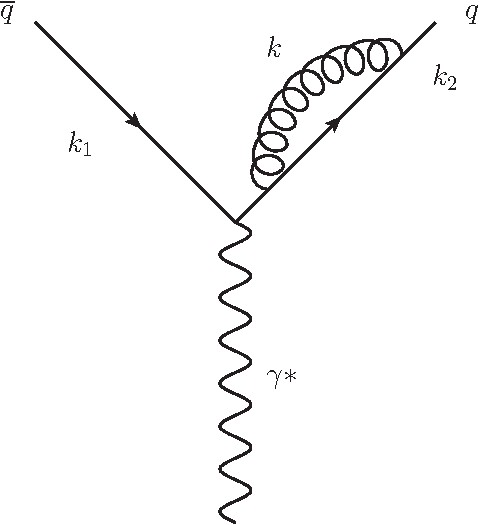
\includegraphics[width=0.8\textwidth]{NLOSelfEnergyRight}
				\caption{$\mathcal{A}_{se2}$}
				\label{fig:NLOfig_4}
			\end{subfigure}
			\begin{subfigure}[b]{0.48\textwidth}
				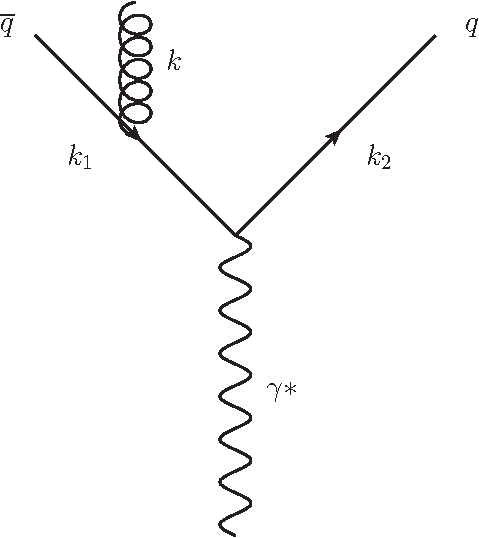
\includegraphics[width=0.8\textwidth]{NLORealLeft}
				\caption{$\mathcal{A}_{r1}$}
				\label{fig:NLOfig_5}
			\end{subfigure}
			\begin{subfigure}[b]{0.48\textwidth}
				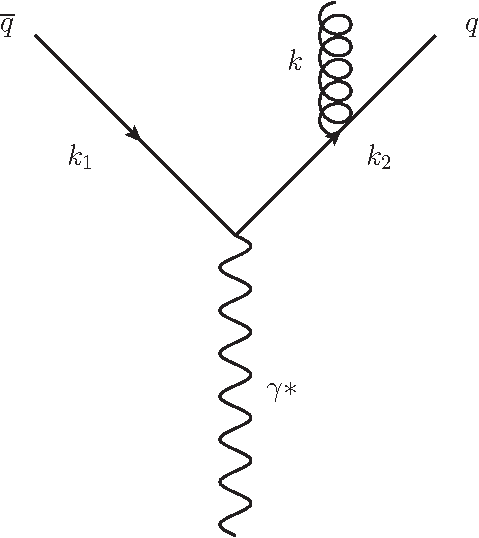
\includegraphics[width=0.8\textwidth]{NLORealRight}
				\caption{$\mathcal{A}_{r2}$}
				\label{fig:NLOfig_6}
			\end{subfigure}

			\caption{Feynman diagrams for calculating the $O(\alpha_s)$ correction to $\gamma^*\rightarrow q\overline{q}$.
			Fig.~\eqref{fig:NLOfig_1} is the leading order contribution.  Figs.~\eqref{fig:NLOfig_2} - \ref{fig:NLOfig_4}
			are the virtual corrections and lastly figs.~\eqref{fig:NLOfig_5} -~\eqref{fig:NLOfig_6} are the real emission
			contributions.}
			\label{fig:NLOContributions}

		\end{figure}

		The Feynman diagrams which need to be included for the and $\mathcal{O}(1)$ and $\mathcal{O}(\alpha_s)$ corrections to the
		$\gamma^*\rightarrow q\overline{q}$ process are shown in fig.~\eqref{fig:NLOContributions}.  We refer to fig.~\eqref{fig:NLOfig_1} as the tree level diagram,
		fig.~\eqref{fig:NLOfig_2} as the vertex correction and figs.~\eqref{fig:NLOfig_3} and~\eqref{fig:NLOfig_4} as the self-energy corrections.
		Figs.~\eqref{fig:NLOfig_5} and~\eqref{fig:NLOfig_6} are the `real corrections'.  Since the virtual corrections all have the same final state
		they must be summed and squared together.  To make the order of each term in the perturbative expansion clear we extract the $\alpha_s$
		factors from the $\mathcal{A}_i$ here.  Therefore:

		\begin{equation}
		\begin{split}
			|\mathcal{M}|^2 = &|\mathcal{A}_0 + \alpha_s\mathcal{A}_v + \alpha_s\mathcal{A}_{se1} + \alpha_s\mathcal{A}_{se2}|^2 + \mathcal{O}(\alpha_s^2) \\
			                = &|\mathcal{A}_0|^2 + 2\alpha_s\Re\{\mathcal{A}^*_0\mathcal{A}_v\} + 2\alpha_s\Re\{\mathcal{A}^*_0\mathcal{A}_{se1}\} \\
			                  & + 2\alpha_s\Re\{\mathcal{A}^*_0\mathcal{A}_{se2}\} + \mathcal{O}(\alpha_s^2),
			\label{eqn:MEBreakdown}
		\end{split}
		\end{equation}

		We can see then that to $\mathcal{O}(\alpha_s)$ we have four contributions to consider, but the two self-energy contributions will have
		the same functional form so it would seem that in practice we only need to perform three calculations - it turns out this is not the
		case; we will find that the divergence associated with exchanging a soft gluon in fig.~\eqref{fig:NLOfig_2} can only be cancelled
		if we also include the soft divergences that arise from figs.~\eqref{fig:NLOfig_5} to~\eqref{fig:NLOfig_6}.  At first glance this
		seems very peculiar since these diagrams have different final states and therefore should have no business contributing to this
		calculation.  However, since the gluon can be emitted with vanishingly small momentum it would be experimentally impossible to
		detect and therefore the final states would look the same to an imperfect observer.\\It is the cancellation of these divergences
		that will be shown in detail in the next two sections.  Figs.~\eqref{fig:NLOfig_1},~\eqref{fig:NLOfig_2} and~\eqref{fig:NLOfig_5}
		will be calculated in detail while the result for the self energy expressions will be omitted since it can be cancelled by
		choosing to work in the Landau gauge~\cite{fieldBook}.  Since we expect both UV and IR divergences we choose to work in the dimensional
		regularisation scheme.

		\subsubsection{The Leading Order Process}

			If we let the pair-produced quarks have charge $\pm Qe$ then the Feynman rules outlined in section \ref{sec:partonicCrossSection} give:

			\begin{equation}
				\mathcal{A}_0 = -ieQ\overline{u}^{\lambda_2}(k_2)\gamma^\mu v^{\lambda_1}(k_1)\epsilon^r_\mu(p),
			\end{equation}

			where we have used the QED Feynman rule for a quark-antiquark-photon vertex: $iQe\gamma^\mu$, the $\lambda_i$'s are the
			spins of the quarks, $r$ is the polarisation of the incoming photon and $p = k_1 + k_2$ is the momentum carried by the
			incoming photon.  To calculate we can square and since we are typically interested in unpolarised calculations we perform
			a sum over all polarisations and spins (we also choose this point to include the sum over the possible colour states of
			the outgoing quarks):

			\begin{equation}
				|\overline{\mathcal{A}_0}|^2 = 3\sum_{\forall\lambda, r}e^2Q^2[\overline{u}^{\lambda_2}(k_2)\gamma^\mu
				v^{\lambda_1}(k_1)][\overline{v}^{\lambda_1}(k_1)\gamma^\nu v^{\lambda_2}(k_1)]\epsilon^r_\mu(p)\epsilon^r_{*\mu}(p).
			\end{equation}

			We can now use Casimir's trick ~\cite{griff} to convert this spinor string into a trace, using the replacements
			$\sum_r\epsilon^r_\mu\epsilon^r_{*\nu}=-g_{\mu\nu}$ and the completeness conditions for spinors:

			\begin{equation}
				|\overline{\mathcal{A}_0}|^2 = - e^2Q^2\Tr[\slashed k_2\gamma^\mu\slashed k_1\gamma_\mu],
			\end{equation}

			where we have used the high energy limit to discard the quark mass terms.  This trace can be evaluated in arbitrary
			dimensions to give, in the high energy limit:

			\begin{equation}
				|\overline{\mathcal{A}_0}|^2 = 6e_d^2Q^2s(d-2),
			\end{equation}

			where we have defined the usual Mandelstam variable $s=(k_1+k_2)^2=2k_1\cdot k_2$ and define $e_d^2=e^2\mu^{4-d}$ where
			$\mu$ has units of mass in order to make the coupling $e$ dimensionless.  To find the leading order cross-section we divide by the
			particle flux and multiply by the two particle phase space which is given by:

			\begin{equation}
				\int d^{2d-2}R_2 = 2^{1-d}\pi^{\frac{d}{2}-1}\frac{\Gamma(\frac{d}{2}-1)}{\Gamma(d-2)}s^\frac{d-4}{2},
			\end{equation}

			where $R_2$ is the two particle phase space in $d$ dimensions.  Combining these factors and defining $\alpha_e=\frac{e^2}{4\pi}$:

			\begin{equation}
			\begin{split}
				\sigma_0 &= 3\cdot2^{2-d}\pi^{1-\frac{d}{2}}\frac{\Gamma(\frac{d}{2}-1)}{\Gamma(d-2)}s^\frac{d-4}{2}4\pi\alpha\mu^{d-4}Q^2s(d-2)\frac{1}{2s} \\
				&= 3\alpha Q^2\left(\frac{s}{4\pi\mu^2}\right)^{\frac{d}{2}-2}\left(\frac{d}{2}-1\right)\frac{\Gamma(\frac{d}{2}-1)}{\Gamma(d-2)}.
			\end{split}
			\end{equation}

			and finally using $x\Gamma(x)=\Gamma(x+1)$ we get:

			\begin{equation}
				\sigma_0 = 3\alpha Q^2 \frac{\Gamma(\frac{d}{2})}{\Gamma(d-2)}\left(\frac{s}{4\pi\mu^2}\right)^{\frac{d}{2}-2}.
				\label{eqn:bornCrossSection}
			\end{equation}

			It is important to note that in the limit $\epsilon\rightarrow0$ the Born cross-section remains finite.

		\subsubsection{The Virtual $\mathcal{O}(\alpha_s)$ Corrections}

			The virtual correction graphs are shown in figs.~\eqref{fig:NLOfig_2},~\eqref{fig:NLOfig_3} and~\eqref{fig:NLOfig_4}.  We will begin by calculating
			the second term in eqn.~\eqref{eqn:MEBreakdown}.  Using the Feynman rules we have:

			\small
				\begin{subequations}
				\begin{align*}
					\mathcal{A}_v = \int\frac{d^{d}k}{(2\pi)^{d}} \overline{u}^{\lambda_2}(k_2)
					(-ig_s\mu^\epsilon\gamma^\alpha T^a_{ij})\frac{i(\slashed k_1 + \slashed k)}{(k_1+k)^2}
					(-ieQ\gamma^\mu)\frac{i(\slashed k_2 - \slashed k)}{(k_2 - k)^2}\\
					(-g_s\mu^\epsilon\gamma^\beta T^a_{ij})
					\epsilon^r_\mu(p)\frac{-i}{k^2}\left(g_{\alpha\beta} +
					(1-\xi)\frac{k^\alpha k^\beta}{k^2}\right)v^{\lambda_1}(k_1).
				\end{align*}
				\begin{align*}
					\mathcal{A}_v = -ig_s^2eQ\mu^{2\epsilon}\Tr(T^aT^a)\overline{u}^{\lambda_2}
					(k_2)\int\frac{d^{d}k}{(2\pi)^{d}}\frac{\mathcal{N}_1(k_1, k_2, k)}{k^2(k_1+k)^2(k_2-k)^2}v^{\lambda_2}(k_2),
				\end{align*}
				\end{subequations}
			\normalsize

			where the numerator of the fraction is given by:

			\begin{equation}
				\mathcal{N}_1(k_1, k_2, k) = \gamma^\alpha(\slashed k_1 + \slashed k)\gamma^\mu(\slashed k_2 -
				\slashed k)\gamma_\beta\Big(g^{\alpha\beta} + (1-\xi)\frac{k^\alpha k^\beta}{k^2}\Big).
			\end{equation}

			From eqn.~\eqref{eqn:MEBreakdown} we see we need $\mathcal{A}_0^*\mathcal{A}_v$:

			\begin{align}
				\mathcal{A}_0^*\mathcal{A}_v = &g_s^2e^2Q^2\Tr(T^aT^a)[\overline{v}^{\lambda_1}(k_1)\gamma^\nu u(k_2)]\\
				&\left[\overline{u}^{\lambda_2}(k_2)\int\frac{d^{d}k}{(2\pi)^{d}}\frac{\mathcal{N}_1(k_1, k_2, k)}
				{k^2(k_1+k)^2(k_2-k)^2}v^{\lambda_1}(k_1)\right]\epsilon^r_{\mu}(p)\epsilon^r_{*\nu}(p).
			\end{align}

			Now performing the spin/polarisation/colour sum and average gives:

			\begin{equation}
				\overline{\mathcal{A}_0^*\mathcal{A}_v} = -\frac{g_s^2e^2Q^2}{2}\int\frac{d^{d}k}
				{(2\pi)^{d}}\frac{\mathcal{N}_2(k_1, k_2,k)}{k^2(k_1+k)^2(k_2-k)^2},
			\end{equation}

			where:

			\begin{equation}
				\mathcal{N}_2(k_1, k_2, k) = \Tr[\slashed k_1 \gamma_\alpha(\slashed k_1 + \slashed k)\gamma_\mu
				(\slashed k_2 - \slashed k)\gamma_\beta\slashed k_2\gamma^\mu]\Big(g^{\alpha\beta} + (1-\xi)\frac{k^\alpha k^\beta}{k^2}\Big).
			\end{equation}

			Before we can proceed any further we must evaluate the trace term in the integral.  As mentioned briefly in section
			\ref{sub:regularising} this is not as easy as it seems because, although the Dirac matrices still satisfy the Clifford
			algebra, the various identities for their contractions and traces change when we are in $d$ dimensions.  Two useful
			examples are shown below:

			\begin{subequations}
				\begin{equation}
				g_{\mu\nu}g^{\mu\nu} = d
				\end{equation}
				\begin{equation}
				\gamma^\mu\gamma_\nu\gamma_\mu = (d-2)\gamma_nu
				\end{equation}
			\end{subequations}

			Using the \texttt{FORM} package ~\cite{form} to perform the two trace terms present gives:

			\begin{equation}
				\begin{split}
				\Tr[\slashed k_1 \gamma_\alpha(\slashed k_1 + \slashed k)\gamma_\mu(\slashed k_2 &-
				\slashed k)\gamma^\alpha\slashed k_2\gamma^\mu] = s[s(8-4d) + \frac{(k_1\cdot k)(k_2\cdot k)}{s}(32-16d) \\
				&- (16-8d)(k_1\cdot k - k_2\cdot k) + k^2(16-12d+2d^2)],
				\end{split}
			\end{equation}

			and,

			\begin{equation}
				\begin{split}
				\Tr[\slashed k_1 \gamma_\alpha(\slashed k_1 + \slashed k)\gamma_\mu(\slashed k_2 &- \slashed k)\gamma_\beta
				\slashed k_2\gamma^\mu]k^\alpha k^\beta = s[(k_1\cdot k)(k_2\cdot k)(16 - 8d) \\
				&+ k^2(8 - 4d)(k_2\cdot k - k_1\cdot k) - k^4(4 - 2d)],
				\end{split}
			\end{equation}

			where $s = 2k_1\cdot k_2$ and we have used the on-shell relations.  After factorising the terms
			quadratic in $d$ and combining the two trace terms we arrive at:

			\begin{equation}
				\overline{\mathcal{A}_0^*\mathcal{A}_v} = -4s\left(\frac{d}{2}-1\right)\frac{g_s^2e^2Q^2}{2}
				\int\frac{d^{d}k}{(2\pi)^{d}}\frac{\mathcal{N}_3(k_1, k_2, k)}{k^2(k_1+k)^2(k_2-k)^2},
			\end{equation}

			where:

			\begin{align}
				\mathcal{N}_3(k_1, k_2, k) = -2s + \frac{8k\cdot k_1k\cdot k_2}{s} + (6+2\xi)(k\cdot k_1 -
				k\cdot k_2) + k^2(d-4) \\- 4(1-\xi)\frac{k\cdot k_1 k\cdot k_2}{k^2} - (1-\xi)k^2.
			\end{align}

			Combining this with the particle flux and the two particle phase space we can write an expression
			for the vertex corrected cross-section.  Once again we scale the couplings such that they remain
			dimensionless by defining $g_d^2=g_s^2\mu^{2-\frac{d}{2}}$:

			\begin{subequations}
				\begin{equation*}
				\sigma_v = -4s\left(\frac{d}{2}-1\right)\frac{g_d^2\mu^{2-\frac{d}{2}}e^2Q^2}{4s}2^{1-d}\pi^{\frac{d}{2}-1}
				\frac{\Gamma(\frac{d}{2}-1)}{\Gamma(d-2)}s^\frac{d-4}{2}\int\frac{d^{d}k}{(2\pi)^{d}}\frac{\mathcal{N}_3(k_1, k_2, k)}{k^2(k_1+k)^2(k_2-k)^2},
				\end{equation*}
				\begin{equation*}
				\Rightarrow\sigma_v = -g_d^2\mu^{2-\frac{d}{2}}Q^2 4\pi\alpha\mu^{4-d}2^{1-d}\pi^{\frac{d}{2}-1}\frac{\Gamma(
				\frac{d}{2})}{\Gamma(d-2)}s^\frac{d-4}{2}\int\frac{d^{d}k}{(2\pi)^{d}}\frac{\mathcal{N}_3(k_1, k_2, k)}{k^2(k_1+k)^2(k_2-k)^2},
				\end{equation*}
				\begin{equation*}
				\Rightarrow\sigma_v = -\frac{4\sigma_0}{3}g_d^2\mu^{2-\frac{d}{2}}\int\frac{d^{d}k}{(2\pi)^{d}}
				\frac{\mathcal{N}_3(k_1, k_2, k)}{k^2(k_1+k)^2(k_2-k)^2},
				\end{equation*}
			\end{subequations}

			where we have expressed the virtual rate as a multiplicative correction to the Born level rate
			by comparing directly with eq. (35).  We must now use the Feynman parametrisation to re-express
			the product of propagators as a sum by introducing new integration variables.  Using:

			\begin{equation}
				\frac{1}{ab} = \int_0^1dy\frac{1}{(ay+b(1-y))^2},
				\label{eqn:usefulParam}
			\end{equation}

			we have:

			\begin{equation}
				\sigma_v = -\frac{4\sigma_0}{3}g_d^2\mu^{2-\frac{d}{2}}\int\frac{d^{d}k}{(2\pi)^d}
				\int_0^1dy\frac{\mathcal{N}_3(k_1, k_2, k)}{(k^2-2k\cdot k_y)^2k^2},
			\end{equation}

			where $k_y = yk_1 -(1-y)k_2$.  Examining now the integrand we see there are two
			different $k$ dependences and so we partition the terms as follows:

			\begin{equation}
				\sigma_v = -\frac{4\sigma_0}{3}g_d^2\mu^{2-\frac{d}{2}}\int\frac{d^{d}k}{(2\pi)^d}\int_0^1dy
				\left(\frac{\mathcal{N}'_3(k_1, k_2, k)}{(k^2-2k\cdot k_y)^2k^2} +
				\frac{\mathcal{N}''_3(k_1, k_2, k)}{(k^2-2k\cdot k_y)^2k^4}\right),
			\end{equation}

			where,

			\begin{subequations}
				\begin{equation}
					\mathcal{N}'_3(k_1, k_2, k) = -2s + \frac{8k\cdot k_1k\cdot k_2}{s} +
					(6+2\xi)(k\cdot k_1 - k\cdot k_2) + k^2(d-4) - (1-\xi)k^2.
				\end{equation}
					\begin{equation}
					\mathcal{N}''_3(k_1, k_2, k) = - 4(1-\xi)k\cdot k_1 k\cdot k_2.
				\end{equation}
			\end{subequations}

			Differentiating eqn.~\eqref{eqn:usefulParam} with respect to $a$ and $b$ we get the following useful parametrisations:

			\begin{subequations}
				\begin{equation}
				\frac{1}{a^2b} = \int_0^1dx\frac{2x}{(ax+b(1-x))^3},
				\end{equation}
				\begin{equation}
				\frac{1}{a^2b^2} = \int_0^1dx\frac{6x(1-x)}{(ax+b(1-x))^4}.
				\end{equation}
			\end{subequations}

			and taking $a = k^2-2k\cdot k_y$ and $b = k^2$, simplifying the denominators and performing a change of variables $K=k-xp_y$ yields:

			\begin{align}
				\sigma_v = -\frac{4\sigma_0}{3}g_d^2\mu^{2-\frac{d}{2}}\int\frac{d^{d}K}{(2\pi)^d}\int_0^1dy\int_0^1dx
				\Bigg(&\frac{2x\mathcal{N}'_3(k_1, k_2, K+xk_y)}{(K^2-C)^3} + \\&\frac{6x(1-x)
				\mathcal{N}''_3(k_1, k_2, K+xk_y)}{(K^2-C)^4}\Bigg),
			\end{align}

			where $C = x^2p_y^2$.  The change of variables modifies the numerator terms to:

			\begin{subequations}
				\begin{align}
				\begin{split}
					\mathcal{N}'_3(k_1, k_2, K+xk_y) = &-2s + K^2\Big(\frac{4}{d} + d - 5 + \xi\Big) \\ &- (3 + \xi)xs + x^2ys(1-y)(3-d-\xi),
					\label{eqn:numeratorTerms1}
				\end{split}
				\end{align}
				\begin{equation}
				\mathcal{N}''_3(k_1, k_2, K+xk_y) = (1-\xi)\left(x^2ys^2(1-y)-\frac{2s}{d}K^2\right).
				\label{eqn:numeratorTerms2}
				\end{equation}
				\label{eqn:numeratorTerms}
			\end{subequations}

			We can now perform the integrations over $K$ with the aid of the following result:

			\begin{equation}
				\int\frac{d^{d}K}{(2\pi)^d}\frac{(K^2)^m}{(K^2-C)^n} = \frac{i(-1)^{m-n}}{(4\pi)^\frac{d}{2}}
				C^{m-n+\frac{d}{2}}\frac{\Gamma(m+\frac{d}{2})\Gamma(n-m-\frac{d}{2})}{\Gamma(\frac{d}{2})\Gamma(n)}.
				\label{eqn:eqn54}
			\end{equation}

			Looking at the $K$ structure of eqs.~\eqref{eqn:numeratorTerms} we can see that there are going to be 4 forms
			of eqn.~\eqref{eqn:eqn54} needed in this calculation.  I will not show the calculation for every integral
			but will show one as an example of how the calculations can proceed.  Consider the contribution of the first
			term of eqn.~\eqref{eqn:numeratorTerms1}:

			\begin{equation*}
				 I = -4s\int_0^1dy\int_0^1dxx\int\frac{d^{d}K}{(2\pi)^d}\frac{1}{(K^2-C)^3} = 4si\int_0^1dy\int_0^1dxx(4\pi)^{-\frac{d}{2}}
				C^{-3+\frac{d}{2}}\frac{\Gamma(\frac{d}{2})\Gamma(3-\frac{d}{2})}{\Gamma(\frac{d}{2})\Gamma(3)}.
			\end{equation*}

			From above we see that $C=x^2k_y=-x^2y(1-y)s$ and so:

			\begin{align}
			\begin{split}
				I = 4si(4\pi)^{-\frac{d}{2}}\Gamma(3-\frac{d}{2})(-s)^{-3+\frac{d}{2}}\int_0^1dy\int_0^1dxx^{-5+d}
				y^{\left(-2+\frac{d}{2}\right)-1}(1-y)^{\left(-2+\frac{d}{2}\right)-1},
			\end{split}
			\end{align}

			Therefore:

			\begin{equation}
				I = 4si(4\pi)^{-\frac{d}{2}}\Gamma\left(3-\frac{d}{2}\right)(-s)^{-3+\frac{d}{2}}
				\frac{1}{d-4}\frac{\Gamma^2(\frac{d}{2}-2)}{\Gamma(d-4)}.
			\end{equation}

			Choosing $d=4+\epsilon$ (with the intention of taking the limit $\epsilon\rightarrow0$
			once it is safe to do so), and manipulating the gamma functions to expose the pole structure gives:

			\begin{equation}
				-4\int_0^1dy\int_0^1dxx\int\frac{d^{d}K}{(2\pi)^d}\frac{1}{(K^2-C)^3} = 4(-s)^{\frac{\epsilon}{2}}i(4\pi)^{-2-\frac{\epsilon}{2}}
				\frac{4}{\epsilon^2}\frac{\Gamma\left(1-\frac{\epsilon}{2}\right)\Gamma^2\left(1+\frac{\epsilon}{2}\right)}{\Gamma(1+\epsilon)},
			\end{equation}

			which is clearly divergent in the limit $d\rightarrow4$.  The other integrals follow similarly and
			the combined result can be expressed as:

			\begin{equation}
				\sigma_v = \frac{2\alpha_s}{3\pi}\sigma_0\Big(\frac{s}{4\pi\mu^2}\Big)^{\frac{\epsilon}{2}}\frac{\Gamma
				\Big(1-\frac{\epsilon}{2}\Big)\Gamma^2\Big(1+\frac{\epsilon}{2}\Big)}{\Gamma(1+\epsilon)}\Big(-\frac{8}{\epsilon^2} +
				\frac{6}{\epsilon} - \frac{8+4\epsilon}{1+\epsilon}\Big),
			\end{equation}

			where we have defined $\alpha_s=\frac{g_d^2}{4\pi}$. Expanding the product of gamma matrices for $\epsilon\rightarrow0$
			gives:

			\begin{subequations}
				\begin{equation}
				\frac{\Gamma\left(1-\frac{\epsilon}{2}\right)\Gamma^2\left(1+\frac{\epsilon}{2}\right)}{\Gamma(1+\epsilon)} =
				\frac{\gamma_E}{2}\epsilon + \left(\frac{\gamma_E^2}{8} - \frac{\pi^2}{48}\right)\epsilon^2 + \mathcal{O}(\epsilon^3),
				\end{equation}
				\begin{equation}
				\left(\frac{s}{4\pi\mu^2}\right)^{\frac{\epsilon}{2}} = e^{\ln{\left(\frac{s}{4\pi\mu^2}\right)^{\frac{\epsilon}{2}}}} =
				e^{\frac{\epsilon}{2}\ln\left(\frac{s}{4\pi\mu^2}\right)} = 1 + \frac{\epsilon}{2}\ln\left(\frac{s}{4\pi\mu^2}\right) + \mathcal{O}(\epsilon^2),
				\end{equation}
			\end{subequations}

			where $\gamma_E$ is Euler's constant.  Finally then we have:

			\begin{align}
				\sigma_v = \frac{2\alpha_s}{3\pi}\sigma_0\Big[&-\frac{8}{\epsilon^2} + \frac{1}{\epsilon}\left(6-4\gamma_E-4L\right) +
				\gamma_E(3-\gamma_E)\\&-8+\frac{\pi^2}{6}+\pi^2-L^2-(2\gamma_E-3)L\Big],
			\end{align}

			where $L = \ln{\left(\frac{s}{4\pi\mu^2}\right)}$.  We can now see that regardless of our choice of
			gauge parameter, $\xi$, the result for the vertex correction is gauge independent.  We also see that
			the parameter introduced to fix the coupling to be dimensionless appears in the final result;  this
			is often the case when using dimensional regularisation and the modified minimal subtraction renormalisation scheme.

		\subsubsection{The Real $\mathcal{O}(\alpha_s)$ Corrections}

			The real gluon emission diagrams which contribute to the $\mathcal{O}(\alpha_s)$ corrections are
			figs.~\eqref{fig:NLOfig_5} and~\eqref{fig:NLOfig_6}.  These diagrams have an indistinguishable final state and so the real contribution will be of the form:

			\begin{equation}
				|\mathcal{A}_r|^2 = |\mathcal{A}_{left} + \mathcal{A}_{right}|^2 =
				|\mathcal{A}_{left}|^2 + |\mathcal{A}_{right}|^2 + 2\mathcal{A}_{left}\mathcal{A}_{right}^*,
			\end{equation}

			where $\mathcal{A}_{left}$ and $\mathcal{A}_{right}$ refer to figs.~\eqref{fig:NLOfig_5} and~\eqref{fig:NLOfig_6} respectively and are given by:

			\begin{subequations}
				\begin{equation}
				\mathcal{A}_{left} = -Qeig_sT^a_{ij}\overline{u}(k_2)\gamma^\mu\frac{\slashed k_1 + \slashed k}{(k_1 + k)^2}\gamma^\nu v(k_1)\epsilon_\nu\eta_\mu,
				\end{equation}
				\begin{equation}
				\mathcal{A}_{right} = -Qeig_sT^a_{ij}\overline{u}(k_2)\gamma^\nu\frac{\slashed k_2 + \slashed k}{(k_2 + k)^2}\gamma^\mu v(k_1)\epsilon_\nu\eta_\mu.
				\end{equation}
			\end{subequations}

			In the calculation of the terms of eq. (64) it will be useful to write the energy fractions for each
			particle as $x_i = \frac{2E_i}{\sqrt{s}}$ (where $i=1$ is the external antiquark, $i=2$ is the antiquark
			and $i=3$ is the external gluon).  In terms of these invariants the contraction of any two external
			particles simplifies to $p_i\cdot p_j = \frac{1}{2}s(1-x_k)$ which (since we are still assuming our
			quarks can be taken to be massless) gives a simple expression for the Mandelstam variables.
			Evaluating the $|...|^2$ terms gives:

			\begin{subequations}
				\begin{equation}
				|\mathcal{A}_{left}|^2  = \frac{Q^2e^2g_s^2}{(k_1+k)^4}\Tr(T^aT^a)\Tr(\slashed k_2 \gamma^\mu (\slashed k_1 + \slashed k)
				\gamma^\nu \slashed k_1 \gamma_\nu (\slashed k_1 + \slashed k) \gamma_\mu),
				\end{equation}
				\begin{equation}
				|\mathcal{A}_{right}|^2 = \frac{Q^2e^2g_s^2}{(k_2+k)^4}\Tr(T^aT^a)\Tr(\slashed k_2 \gamma^\nu (\slashed k_2 + \slashed k)
				\gamma^\mu \slashed k_2 \gamma_\mu (\slashed k_2 + \slashed k) \gamma_\nu),
				\end{equation}
				\begin{equation}
				\mathcal{A}_{left}\mathcal{A}_{right}^* = \frac{Q^2e^2g_s^2}{(k_2+k)^2(k_1+k)^2}\Tr(T^aT^a)\Tr(\slashed k_2\gamma^\mu
				(\slashed k_1 + \slashed k) \gamma^\nu \slashed k_1 \gamma_\mu (\slashed k_2 + \slashed k) \gamma_\nu).
				\end{equation}
			\end{subequations}

			Evaluating the trace terms in $d$-dimensions and rearranging in terms of the energy fractions gives:

			\begin{subequations}
				\begin{equation}
				|\mathcal{A}_{left}|^2  = 32Q^2e^2g_s^2\left(1+\frac{\epsilon}{2}\right)^2\frac{1-x_1}{1-x_2},
				\end{equation}
				\begin{equation}
				|\mathcal{A}_{right}|^2 = 32Q^2e^2g_s^2\left(1+\frac{\epsilon}{2}\right)^2\frac{1-x_2}{1-x_1},
				\end{equation}
				\begin{equation}
				2\mathcal{A}_{left}\mathcal{A}_{right}^* = 64Q^2e^2g_s^2\left(1+\frac{\epsilon}{2}\right)\left(-\frac{\epsilon}{2}-2\frac{1-x_3}{(1-x_1)(1-x_2)}\right).
				\end{equation}
			\end{subequations}

			Summing these expressions gives:

			\begin{equation}
				|\mathcal{A}_r|^2 = 32Q^2e^2g_s^2\left[\left(1+\frac{\epsilon}{2}\right)^2\frac{x_1^2+x_2^2}{(1-x_2)(1-x_1)} +
				\epsilon\left(1+\frac{\epsilon}{2}\right)\frac{2-2x_1-2x_2+x_1x_2}{(1-x_2)(1-x_1)}\right].
				\label{eqn:eqn67}
			\end{equation}

			As with the virtual contributions we are interested in the observable cross-section and so we must
			include the phase space factor for a three particle final state.  Unlike the two particle phase space
			calculation here $\int d^{3d-3}R_3$ cannot be integrated completely and we are left with a
			differential in terms of the energy fractions defined above:

			\begin{equation}
				\frac{d^2R_3}{dx_1dx_2} = \frac{s}{16(2\pi)^3}\left(\frac{s}{4\pi}\right)^\epsilon\frac{1}{\Gamma(2+\epsilon)}
				\left(\frac{1-z^2}{4}\right)^{\frac{\epsilon}{2}}x_1^\epsilon x_2^\epsilon,
				\label{eqn:eqn68}
			\end{equation}

			where $z = 1 - 2\frac{1-x_1-x_2}{x_1x_2}$.  Combining eqs.~\eqref{eqn:eqn67} and~\eqref{eqn:eqn68} with a flux factor gives:

			\begin{equation}
				\frac{d^2\sigma_r}{dx_1dx_2} = \frac{2Q^2e^2g_s^2F(x_1, x_2; \epsilon)}{\pi}\left(\frac{s}{4\pi}\right)^\epsilon
				\frac{1}{\Gamma(2+\epsilon)}\left(\frac{1-z^2}{4}\right)^{\frac{\epsilon}{2}}x_1^\epsilon x_2^\epsilon,
			\end{equation}

			where we define $F(x_1, x_2; \epsilon)$ as the algebraic factor in square brackets from eqn.~\eqref{eqn:eqn67}.  Switching to
			a dimensionless coupling and introducing $\alpha_s$ as above:

			\begin{equation}
				\frac{d^2\sigma_r}{dx_1dx_2} = \frac{2Q^2e^2\alpha_s}{\pi}F(x_1, x_2; \epsilon)\left(\frac{s}{4\pi\mu^2}\right)^\epsilon
				\frac{1}{\Gamma(2+\epsilon)}\left(\frac{1-z^2}{4}\right)^{\frac{\epsilon}{2}}x_1^\epsilon x_2^\epsilon.
			\end{equation}

			Comparing with the Born cross-section in eqn.~\eqref{eqn:bornCrossSection} this can be written as:

			\begin{equation}
				\frac{d^2\sigma_r}{dx_1dx_2} = \frac{2\alpha_s\sigma_0}{3\pi}F(x_1, x_2; \epsilon)\left(\frac{s}{4\pi\mu^2}\right)^
				{\frac{\epsilon}{2}}\frac{1}{\Gamma(2+\frac{\epsilon}{2})}\left(\frac{1-z^2}{4}\right)^{\frac{\epsilon}{2}}x_1^\epsilon x_2^\epsilon.
			\end{equation}

			Integrating over the allowed region of $x_1$ and $x_2$:

			\begin{equation}
				\sigma_r = \frac{2\alpha_s\sigma_0}{3\pi}\left(\frac{s}{4\pi\mu^2}\right)^{\frac{\epsilon}{2}}\frac{1}{\Gamma(2+\frac{\epsilon}{2})}
				\int_0^1dx_1x_1^\epsilon\int^1_{1-x_1}x_2^\epsilon\left(\frac{1-z^2}{4}\right)^{\frac{\epsilon}{2}}F(x_1, x_2;\epsilon).
				\label{eqn:eqn72}
			\end{equation}

			We can define a change of variables $x_2=1-vx_1$ to decouple these integrals since:

			\begin{align}
				\left(\frac{1-z^2}{4}\right)^{\frac{\epsilon}{2}} = &\frac{x_1^2(1+v^2)-2vx_1+1}{(1-x_1)x_1v} + \epsilon\frac{x_1^2(1-v+v^2-x_1+1)}
				{(1-x_1)x_1v} \\&+\frac{\epsilon^2}{4}\frac{x_1^2(v^2-2v+1) + 4(v-1) + 1}{(1-x_1)xv}.
			\end{align}

			Substituting this into eqn.~\eqref{eqn:eqn72} and performing the $x_1$ and $v$ integrations gives:

			\begin{equation}
				\sigma_r = \frac{2\alpha_s\sigma_0}{3\pi}\left(\frac{s}{4\pi\mu^2}\right)^{\frac{\epsilon}{2}}\frac{\Gamma^2
				\left(1+\frac{\epsilon}{2}\right)}{\Gamma\left(1+\frac{3\epsilon}{2}\right)}\left[\frac{8}{\epsilon^2} - \frac{6}{\epsilon} + \frac{19}{2}\right].
			\end{equation}

			Further expanding the Gamma functions gives:

			\begin{equation*}
				\sigma_r = \frac{2\alpha_s}{3\pi}\sigma_0\left[\frac{8}{\epsilon^2} + \frac{1}{\epsilon}\left(-6+4\gamma_E+4L\right)-
				\gamma_E(3-\gamma_E)-\frac{57}{6}+\frac{7\pi^2}{6}+L^2+(2\gamma_E-3)L\right].
			\end{equation*}

			As in the case of the virtual corrections this is divergent in the limit $\epsilon\rightarrow0$ and exhibits a residual
			dependence on $\mu$.

		\subsubsection{Cancellation of divergences}

			Having now found the vertex corrections and the real corrections up to $\mathcal{O}(\epsilon^2)$
			we can write the next-to-leading order cross-section by simply summing the two:

			\begin{align}
				\sigma_{NLO} &= \sigma_r + \sigma_v = \frac{\alpha_s}{\pi}\sigma_0.
			\end{align}

			So the total cross-section to next-to-leading order accuracy is:

			\begin{align}
				\sigma &= \sigma_0\left(1 + \frac{\alpha_s}{\pi}\right) + \mathcal{O}(\alpha_s^2).
			\end{align}


			The fact that the infrared divergences in both the real and virtual emission NLO diagrams cancel is an example of the
			KLN theorem which states that the Standard Model is completely free of infrared divergences on the whole and holds
			true at all orders.

	\subsection{Resumming Higher-Order Corrections}

		So as we have seen we can evaluate the truncated perturbative series and, provided we remember to include higher
		multiplicity diagrams which contribute in the soft limit, we will be left with a finite result which is invariant
		under gauge transformations.\\ It would seem then that this is the best way to proceed: we calculate as many corrections
		as we can and reason that all of the higher-order terms we have neglected are suppressed by powers of a small expansion
		parameter - the strong coupling, $\alpha_s$.  If this is indeed the case we should see that each time we go to a higher-order
		in perturbation theory our series begins to converge.  For example the effect of the NLO terms should be small with respect
		to the LO terms etc.  It turns out that this is not true for all observables.  To motivate this we can give a schematic expansion
		of some variable we wish to calculate, $\mathcal{O}$:

		\begin{align}
		\begin{split}
			\mathcal{O} = &\alpha_s  \left(a_1L^2 + b_1L   + c_11\right) + \\
			              &\alpha_s^2\left(a_2L^4 + b_2L^3 + c_2L^2 + d_2L   + e_21\right) + \\
			              &\alpha_s^3\left(a_3L^6 + b_3L^5 + c_3L^4 + d_3L^3 + e_3L^2 + f_3L + g_31\right) + \ldots,
			\label{eqn:schematicExpn}
		\end{split}
		\end{align}

		where $L$ is some logarithm which may be large.  A fixed-order scheme aims to exactly calculate some of the rows of equation
		\eqref{eqn:schematicExpn} under the assumption that all subsequent lines are sufficiently suppressed.  The problem with this
		picture is that the logarithms may be large enough that $\alpha_s^nL^{2n}\sim\mathcal{O}(1)$.  In this case it would appear
		that it would be better for us to calculate the first column of the terms (called the `leading logarithmic' or LL
		approximation) than to find the first \emph{row} of terms (the LO approximation).\\Fig.~\eqref{fig:higgsratios} shows how
		the ratio of the inclusive Higgs plus three jet cross-section to inclusive Higgs plus two jet cross-section varies as
		a function of the rapidity gap between the two leading jets in $p_T$ \cite{jeppeTalk}.  The \texttt{HEJ} prediction is formally leading-logarithmic
		accurate (with leading-order matching for final states with up to three jets) while \texttt{MCFM} is formally next-to-leading order
		accurate.  It is shown in chapter \ref{chap:HEQCD} that this rapidity gap is approximately equal to the logarithm, $L$, which
		we claim violates the key assumptions underlying fixed-order perturbation theory.  Hence, as we move to large $\Delta y(j_1, j_2)$
		we increase the size of $L$ in eqn.~\eqref{eqn:schematicExpn} and the terms neglected by the fixed-order scheme (but captured by a
		LL calculation) grow in size.  The ratio of the inclusive $(n+1)$-jets to $n$-jet cross-sections is an interesting probe of the
		convergence of the QCD perturbative expansion since we are directly comparing the size of the NLO contributions to the LO terms.
		Fig.~\eqref{fig:hJetsRatio1} shows that at a centre-of-mass energy of $14$ TeV (the energy scales soon to be achieved at the LHC)
		even at modest rapidity intervals of around $4.0$ we see that half of all events contain extra radiation and when we pull the leading
		jets apart further in rapidity this increases to three quarters of all events.\\ Furthermore, figs.~\eqref{fig:hJetsRatio2} and
		\eqref{fig:hJetsRatio3} show that as we increase the centre-of-mass energy to that of a potential hadronic future circular
		collider, $33$ TeV and $100$ TeV respectively, these enhanced higher-order terms become even more important - in the extreme case
		of dijets with a separation of $\Delta y(j_1, j_2)\approx8.0$ at a $100$ TeV collider almost \emph{90\%} of the cross-section is
		coming from the next-to-leading term in the perturbative series: this is clear evidence that is not generally sufficient to think
		of the expansion as being controlled by only the strong coupling constant, $\alpha_s$.  We can also test this against existing; fig.
		\eqref{fig:d0wjets} show the probability of extra jet activity in inclusive $W^\pm$ plus dijets as function of the rapidity gap
		between the two leading jets \emph{in rapidity}, $\Delta y(j_F, j_B)$, taken from a very detailed study by the D$\oldemptyset$
		collaboration \cite{Abazov:2013gpa} at the Tevatron experiment.  This is equivalent to the ratio of the inclusive $3j$ and
		inclusive $2j$ cross-sections described in fig.~\eqref{fig:higgsratios}.  We observe the same behaviour that as we pull apart
		the dijets we see a marked rise in the probability of extra emissions but, more importantly, we see that the data show this
		strongly increasing trend too.

		The remaining chapters of this thesis will focus on deriving a formalism for calculating these higher-order corrections in order
		to describe physics observed at the LHC.

		\begin{figure}[tpb]
			\captionsetup[subfigure]{oneside, margin={1cm, 0cm, 0cm}}
			\centering
			\hspace{-0.8cm}
			\begin{subfigure}[b]{0.7\textwidth}
				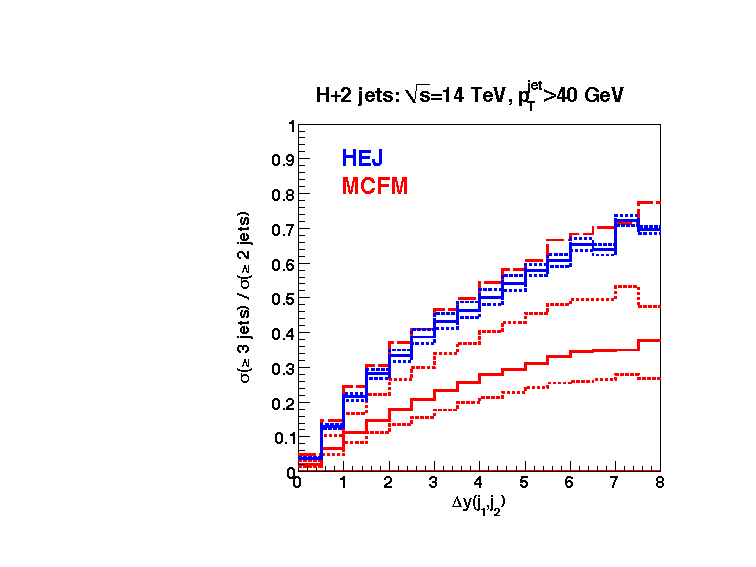
\includegraphics[width=1.0\textwidth]{hJetsRatio1}
				\caption{}
				\label{fig:hJetsRatio1}
			\end{subfigure}
			\captionsetup[subfigure]{oneside,margin={0cm,0cm}}
			\begin{subfigure}[b]{0.48\textwidth}
				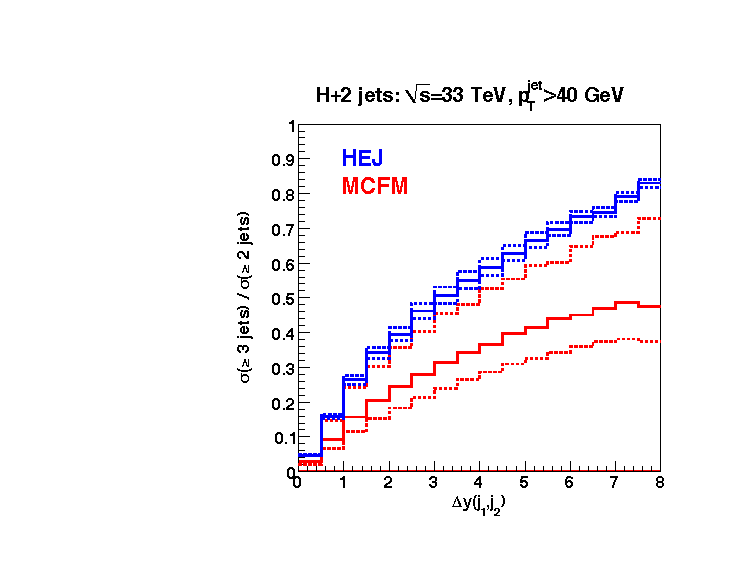
\includegraphics[width=1.0\textwidth]{hJetsRatio2}
				\caption{}
				\label{fig:hJetsRatio2}
			\end{subfigure}
			\begin{subfigure}[b]{0.48\textwidth}
				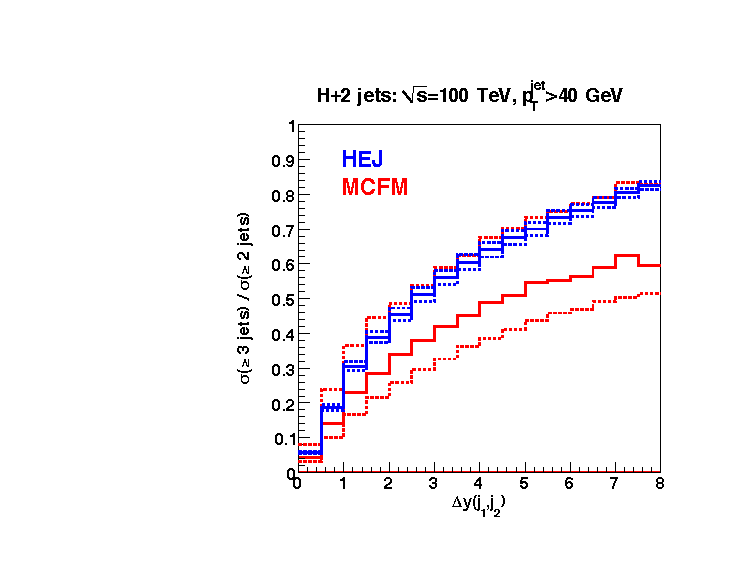
\includegraphics[width=1.0\textwidth]{hJetsRatio3}
				\caption{}
				\label{fig:hJetsRatio3}
			\end{subfigure}

			\caption{The ratio of the inclusive Higgs plus three jet cross-section to inclusive Higgs plus two jet cross-section
			         shown for centre-of-mass energies of $14$TeV (similar to the current LHC), $33$TeV and $100$TeV (possible
			         energy scales for a hadronic future circular collider).}

			\label{fig:higgsratios}
		\end{figure}

		\begin{figure}[hbtp]
			\centering
			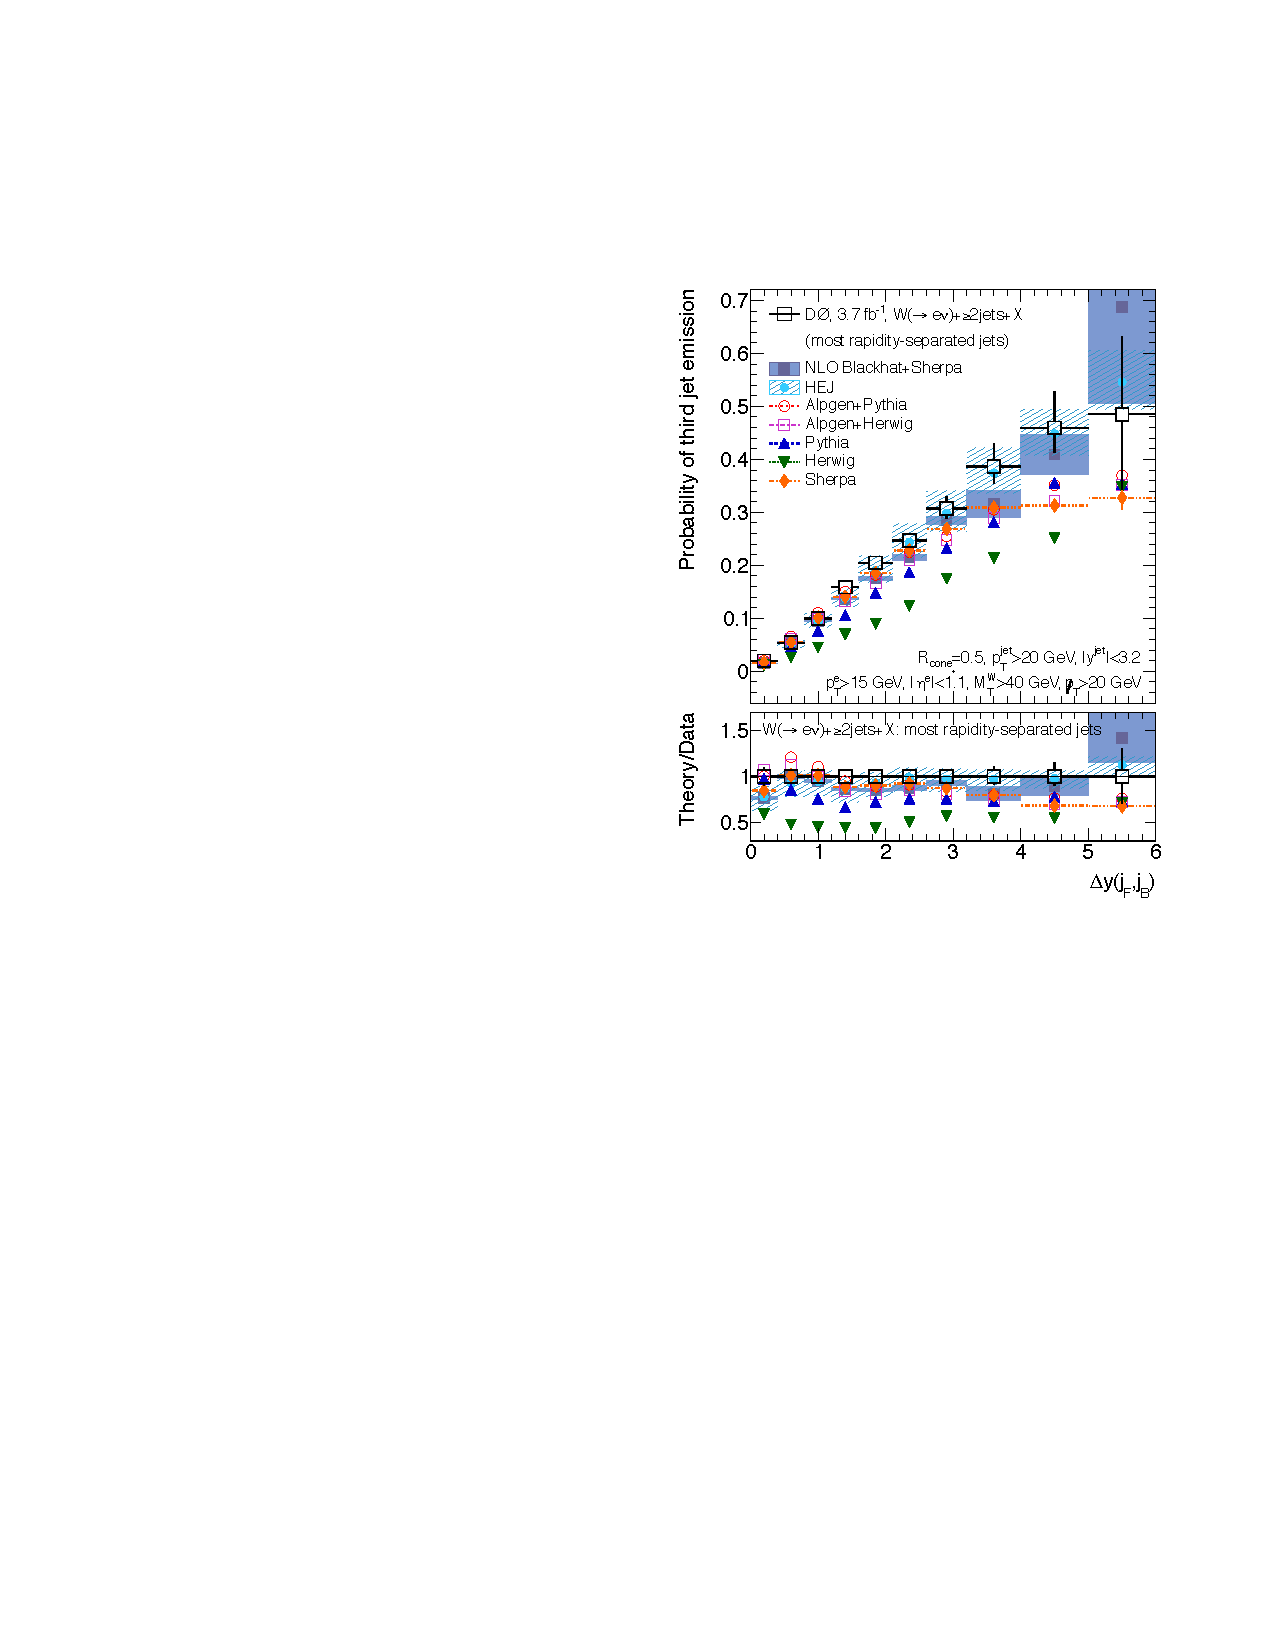
\includegraphics[width=0.75\textwidth]{d0wjets}
			\caption{The probability of a third jet emission in $W^\pm$ plus inclusive dijets as a function of the rapidity gap
			         between the two leading jets in rapidity at the D$\oldemptyset$ experiment at the Tevatron experiment.
			         The data are compared to a number of generators including the leading logarithmic accurate \texttt{HEJ}
			         and the NLO accurate \texttt{Blackhat+Sherpa}.}
			\label{fig:d0wjets}
  		\end{figure}

\section{Spinor-Helicity Notation}
	\label{sec:SpinorHelicity}

	We now move towards the more mechanical aspects of this thesis to discuss a technique which eases calculations.
	In chapters \ref{chap:HEQCD} and \ref{chap:Zs} we choose to work in the spinor-helicity formalism \cite{Dixon:1996wi,CBO9781107706620A004}.
	This is a very convenient choice of notation which allows us to quickly evaluate complicated strings of products of
	Dirac spinors and Dirac matrices which would otherwise be troublesome to work with.\\We begin by looking at the case
	of massless particles; this is relevant for high energy QCD since gluons are massless and the quark masses are often
	negligible compared to the energy scale in a typical scattering process.  The massless Dirac equation can be solved
	by using a plane-wave expansion with some momentum dependent coefficient functions, $u(p)$ and $v(p)$ where $p$ is the
	momentum carried by the particle and must satisfy the on-shell condition $p^2=0$.  This expansion gives the following
	equations:

	\begin{align}
	\begin{split}
		(\slashed p + m)u(p) = 0, \\
		(\slashed p - m)v(p) = 0.
	\end{split}
	\end{align}

	Each of these equations has two independent solutions which we identify as the helicity states, $u^\pm(p)$ and $v^\pm(p)$.
	We use the following notation for these spinors:

	\begin{equation}
		u^\pm(p) = \mid p\pm\rangle, \hspace{1cm} \overline{u^\pm(p)} = \langle p\pm\mid.
	\end{equation}

	In the massless limit we also have the following relation $u^\pm(p) = v^\mp(p)$ which allows us to use the same notation for both
	quarks and anti-quarks.  Often the helicity information will be suppressed in the interests in being concise.  We also define the
	following spinor-brackets:

	\begin{equation}
		\langle pk\rangle = \langle p-\mid k+\rangle, \hspace{1cm} [pk] = \langle p+\mid k-\rangle.
	\end{equation}

	In this language we have the following useful identities:

	\begin{align*}
		\langle ij\rangle[ij] &= s_{ij} & \langle i\pm\mid\gamma^\mu\mid i\pm\rangle &= 2k_i^\mu \\
		\langle ij\rangle &= -\langle ji\rangle & [ij] &= -[ji] \\
		\langle i\pm\mid\gamma^\mu\mid j\pm\rangle\langle k\pm\mid\gamma_\mu\mid l\pm\rangle &=
		2[ik]\langle l j\rangle & \langle k\pm\mid\gamma^\mu\mid l\pm\rangle &=
		\langle l\mp\mid\gamma^\mu\mid k\mp\rangle \\
		\langle i j\rangle\langle k l\rangle &=
		\langle i k\rangle\langle l j\rangle + \langle i l\rangle\langle k j\rangle & [ij][kl] &= [ik][jl]+[il][kj] \\
		\langle i+|\slashed k|j+\rangle &= [ik]\langle kj\rangle & \langle i-|\slashed k|j-\rangle &= \langle ik\rangle [kj]
	\end{align*}

	In the calculations here we use the following convention for spinors.  We express the parton momenta in terms
	of light-cone coordinates where $p^\pm=E\pm p_z$ and $p_{\perp} = p_x + ip_y$.  For outgoing positive (negative) helicity partons,
	$u^+(p)$ ($u^-(p)$) we have:

	\begin{align}
	    u^+(p) &= \begin{pmatrix}
	           \sqrt{p^+} \\
	           \sqrt{p^-}\frac{p_\perp}{|p_\perp|} \\
	           0 \\
	           0 \\
	         \end{pmatrix}\hspace{0.75cm}
	    u^+(p) &= \begin{pmatrix}
	           0 \\
	           0 \\
	           \sqrt{p^-}\frac{p_\perp^*}{|p_\perp|} \\
	           -\sqrt{p^+} \\
	         \end{pmatrix}
	\end{align}

	respectively.  While for incoming positive (negative) helicity partons moving in the positive $z$ direction,
	$u^+(p)$ ($u^-(p)$) we have:

	\begin{align}
	    u^+(p) = \begin{pmatrix}
	           \sqrt{p^+} \\
	           0 \\
	           0 \\
	           0 \\
	         \end{pmatrix}\hspace{0.75cm}
	    u^-(p) = \begin{pmatrix}
	           0 \\
	           0 \\
	           0 \\
	           -\sqrt{p^+} \\
	         \end{pmatrix}
	\end{align}

	respectively.  Lastly for incoming positive (negative) helicity partons moving in the negative $z$ direction,
	$u^+(p)$ ($u^-(p)$) we have:

	\begin{align}
	    u^+(p) &= \begin{pmatrix}
	           0 \\
	           -\sqrt{p^-} \\
	           0 \\
	           0 \\
	         \end{pmatrix}\hspace{0.75cm}
	    u^-(p) &= \begin{pmatrix}
	           0 \\
	           0 \\
	           -\sqrt{p^-} \\
	           0 \\
	         \end{pmatrix}.
	\end{align}

	We also use following form for the Dirac matrices:

	\begin{align}
	    \gamma^0 &= \begin{pmatrix}
	           0 & 0 & 1 & 0\\
	           0 & 0 & 0 & 1\\
	           1 & 0 & 0 & 0\\
	           0 & 1 & 0 & 0\\
	         \end{pmatrix}\hspace{1.2cm}
	    \gamma^1 = \begin{pmatrix}
	           0 & 0 & 0 & -1\\
	           0 & 0 & -1 & 0\\
	           0 & 1 & 0 & 0\\
	           1 & 0 & 0 & 0\\
	         \end{pmatrix}.\\
	    \gamma^2 &= \begin{pmatrix}
	           0 & 0 & 0 & i\\
	           0 & 0 & -i & 0\\
	           0 & -i & 0 & 0\\
	           i & 0 & 0 & 0\\
	         \end{pmatrix}\hspace{0.75cm}
	    \gamma^3 = \begin{pmatrix}
	           0 & 0 & -1 & 0\\
	           0 & 0 & 0 & 1\\
	           1 & 0 & 0 & 0\\
	           0 & -1 & 0 & 0\\
	         \end{pmatrix}.
	\end{align}

	\subsection{Spinor-Helicity Calculations with Massive Partons}
		\label{sub:SMMassive}

		To do calculations with massive partons using the spinor-helicity formalism we must be very careful since all of our favourite
		identities and tricks rely on the spinor brackets, $|i\rangle$, representing massless partons with $p_i^2=0$. We begin by
		defining `fundamental spinors' \cite{spinorThesis} which we can use to build more general spinors and go from there.
		For some $k_0$, $k_1$ satisfying $k_0^2=0$, $k_1^2=-1$ and $k_0\cdot k_1=0$ we can define positive and negative helicity spinors as follows:

		\begin{subequations}
		\begin{align}
			u_{-}(k_0)\overline{u}_-(k_0) &\equiv \omega_- \slashed k_0\\
			u_+(k_0) &\equiv \slashed k_1 u_- (k_0),
		\end{align}
		\label{eqn:definition}
		\end{subequations}

		where $\omega_\lambda = \half(1 + \lambda\gu{5})$ is the helicity projection operator.  In order for these to be valid spinors they must satisfy the following completeness relations:

		\begin{subequations}
			\begin{equation}
				\label{eqn:prop1}
				\sum_\lambda u_\lambda(p)\overline{u}_\lambda(p)=\slashed p + m
			\end{equation}
			\begin{equation}
				\label{eqn:prop2}
				u_\lambda(p)\overline{u}_\lambda (p) = \omega_\lambda\slashed p
			\end{equation}
			\label{eqn:props}
		\end{subequations}

		The spinors in eqn.~\eqref{eqn:definition} can easily be shown to satisfy these as follows:

		\begin{subequations}
		\begin{align*}
			u_-(k_0)\overline{u}_-(k_0) + u_+(k_0)\overline{u}_+(k_0) &= \omega_-\slashed k_0 + \slashed k_1 u_-(k_0)\overline{u}_-(k_0)\slashed k_1,\\
		        &= \omega_-\slashed k_0 + \slashed k_1 \omega_-\slashed k_0\slashed k_1,\\
		        &= \omega_-\slashed k_0 + \half\gu{\mu}k_{1\mu}(1-\gu{5})\gu{\nu}k_{0\nu}\gu{\sigma}k_{1\sigma},\\
		        &= \omega_-\slashed k_0 + \half k_{1\mu}k_{0\nu}k_{1\sigma}(\gu{\mu}\gu{\nu}\gu{\sigma}-\gu{\mu}\gu{5}\gu{\nu}\gu{\sigma}),\\
		        &= \omega_-\slashed k_0 + \half k_{1\mu}k_{0\nu}k_{1\sigma}(2\gu{\mu}g^{\nu\sigma} - \gu{\mu}\gu{\sigma}\gu{\nu}+2\gu{5}\gu{\mu}g^{\nu\sigma} - \gu{5}\gu{\mu}\gu{\sigma}\gu{\nu}),\\
		        &= \omega_-\slashed k_0 + k_{1\mu}k_{0\nu}k_{1\sigma}\omega_+\gu{\mu}(2g^{\nu\sigma} - \gu{\sigma}\gu{\nu}),\\
		        &= \omega_-\slashed k_0 + 2\slashed k_1 k_0\cdot k_1 - \omega_+\slashed k_1\slashed k_1 \slashed k_0,\\
		        &= \omega_-\slashed k_0 + \omega_+\slashed k_0,
		\end{align*}
		\end{subequations}

		where we have used ${\gu{\mu}, \gu{\mu}}=2g^{\mu\nu}$, ${\gu{\mu}, \gu{5}}=0$ and $\slashed k_1\slashed k_1=k_1^2=0$.
		This proves the property of eqn.~\eqref{eqn:props} and inserting the definition of $\omega_\lambda$ gives:

		\begin{subequations}
		\begin{align*}
			u_-(k_0)\overline{u}_-(k_0) + u_+(k_0)\overline{u}_+(k_0) &= \half(1-\gu{5})\slashed k_0 + (1+\gu{5})\slashed k_0,\\
			&= \slashed k_0,
		\end{align*}
		\end{subequations}

		which is eqn.~\eqref{eqn:props} for a massless particle.\\We can use these fundamental spinors
		to form spinors for any given momenta, $p$ (which has $p^2=0$), as follows:

		\begin{equation}
			u_\lambda(p) = \slashed p u_{-\lambda}(k_0) \frac{1}{\sqrt{2p\cdot k_0}},
		\end{equation}

		provided we don't have $p\cdot k_0=0$.  Once again it is easy to show that this spinor satisfies the necessary conditions, for example:

		\begin{subequations}
		\begin{align*}
			u_\lambda(p)\overline{u}_\lambda(p) &= \frac{1}{2p\cdot k_0}\slashed p u_{-\lambda}(k_0)\overline{u}_{-\lambda}(p)\slashed p,\\
			&= \frac{1}{2p\cdot k_0}\slashed p \omega_{-\lambda}\slashed k_0\slashed p,\\
			&= \frac{1}{4p\cdot k_0}\slashed p (1-\lambda\gu{5})\slashed k_0\slashed p,\\
			&= \frac{1}{2p\cdot k_0}p_{\mu}k_{0\nu}p_{\sigma}\omega_{\lambda}\gu{\mu}(2g^{\nu\sigma} - \gu{\sigma}\gu{\nu}),\\
			&= \frac{1}{2p\cdot k_0}\omega_\lambda(2\slashed p p\cdot k_0 - \slashed p\slashed p\slashed k)),\\
			&= \omega_\lambda\slashed p.\\
		\end{align*}
		\end{subequations}

		So far so good.  This can also be generalised so that we can build massive spinors from our fundamental ones.  We can use

		\begin{equation}
			\label{u_def}
			u(q, s) = \frac{1}{\sqrt{2q\cdot k}}(\slashed q + m)u_-(k)
		\end{equation}

		to describe a quark with spin 4-vector $s$, mass $m$ and momentum $q$.  To confirm this we go through the same procedure as above:

		\begin{subequations}
		\begin{align*}
			u_\lambda(p,s)\overline{u}_\lambda(p,s) &= \frac{1}{2q\cdot k_0}(\slashed q + m) u_-(k_0)\overline{u}_-(q)(\slashed q + m),\\
			&= \frac{1}{2q\cdot k_0}(\slashed q + m) \omega_-\slashed k_0 (\slashed q + m), \\
			&= \frac{1}{4q\cdot k_0}(\slashed q + m) (1-\gu{5})\slashed k_0 (\slashed q + m), \\
			&= \frac{1}{4q\cdot k_0}\big[\left(\slashed q \slashed k_0 \slashed q + m\slashed k\slashed q + m\slashed q \slashed
			k_0 + m^2 \slashed k\right)-\gu{5}\left(\slashed q\slashed k\slashed q - m\slashed k\slashed q + m\slashed q\slashed k_0 - m^2\slashed k\right)\big], \\
			&= \half\left(\slashed q + m - \gu{5}\slashed q - m\gu{5} + \frac{m\gu{5}\slashed k\slashed q}{k\cdot q} + \frac{\gu{5}m^2\slashed k}{k\cdot q}\right),\\
			&= \half\left(1+\left(\frac{1}{m}\slashed q - \frac{m}{q\cdot k}\slashed k\right)\gu{5}\right)(\slashed q + m),\\
			&= \half\left(1+\slashed s\gu{5}\right)(\slashed q + m),\\
		\end{align*}
		\end{subequations}

		where the last line defines the spin vector $s = \frac{1}{m} q - \frac{m}{q\cdot k}k$.  Conjecturing
		a similar form for an antiquark spinor with with spin 4-vector $s$, mass $m$ and momentum $q$:

		\begin{equation}
			\label{v_def}
			v(q, s) = \frac{1}{\sqrt{2q\cdot k}}(\slashed q - m)u_-(k)
		\end{equation}

		leads to:

		\begin{subequations}
		\begin{align*}
			v_\lambda(p,s)\overline{v}_\lambda(p,s) &= \frac{1}{2q\cdot k_0}(\slashed q - m) u_-(k_0)\overline{u}_-(q)(\slashed q - m),\\
			&= \half\left(\left(\slashed q - m\right) + \left(-\slashed q + m + \frac{m^2}{q\cdot k_0}\slashed k_0 -
			\frac{m}{q\cdot k_0}\slashed q\slashed k_0 \right)\gu{5}\right), \\
			&= \half\left(1+\slashed s\gu{5}\right)(\slashed q - m).\\
		\end{align*}
		\end{subequations}

		One last check that is worth performing is that these spinors actually satisfy the Dirac
		equation for both the quark and antiquark case.  For the quark:

		\begin{subequations}
		\begin{align*}
			\slashed q u(q, s) &= \frac{1}{2q\cdot k_0}\slashed q(\slashed q + m)u_-(k_0), \\
			                   &= \frac{1}{2q\cdot k_0}(m^2 + m\slashed q)u_-(k_0). \\
		\end{align*}
		\end{subequations}

		We now define some momentum $\widetilde{q}$ through the relation $q = \widetilde{q} + k_0$ such that $\widetilde{q}^2=0$ and
		$q\cdot k = \widetilde{q}\cdot k$.  Since $q^2=2\widetilde{q}\cdot k=m^2$ we may write

		\begin{subequations}
		\begin{align*}
			\slashed q u(q, s) &= \frac{1}{m}(m^2 + m\slashed q)u_-(k_0), \\
			                   &= (m + \slashed q)u_-(k_0). \\
		\end{align*}
		\end{subequations}

		We can now back substitute from the definition of $u(q, s)$ in eq. \eqref{u_def} to get:

		\begin{subequations}
		\begin{align*}
			\slashed q u(q, s) &= \sqrt{2q\cdot k}u(q, s), \\
			                   &= mu(q,s), \\
		\end{align*}
		\end{subequations}

		which is the Dirac equation for a quark.  The result for antiquarks follows similarly.
		Now we have forms for massive quarks and antiquarks in terms of massless spinors we can
		use all of the spinor-helicity machinery to make our computations more efficient.  Slightly
		more useful forms of equations \eqref{u_def} and \eqref{v_def} can be found by decomposing $q$
		into massless components once again: $q=\widetilde{q}+k$.  Then from eq. \eqref{u_def}:

		\begin{subequations}
		\begin{align*}
			u(q, s) &= \frac{1}{m}(\slashed{\widetilde{q}} + \slashed{k} + m)u_-(k), \\
			        &= \frac{1}{m}\left(\rl{\widetilde{q}^+}{\widetilde{q}^+}k^-\rangle +
			        \rl{\widetilde{q}^-}{\widetilde{q}^-}k^-\rangle + \rl{k^-}{k^-}k^-\rangle +
			        \rl{k^-}{k^-}k^-\rangle + m|k^-\rangle\right), \\
			        &= \frac{[\widetilde{q}k]}{m}|\widetilde{q}^+\rangle + |k^-\rangle,
		\end{align*}
		\end{subequations}

		and similarly for the other helicities and the antiquarks:

		\begin{subequations}
		\begin{align}
			u(q, -s) &= \frac{\langle \widetilde{q}k\rangle}{m}|\widetilde{q}^-\rangle + |k^+\rangle, \\
			v(q,  s) &= \frac{[\widetilde{q}k]}{m}|\widetilde{q}^+\rangle - |k^-\rangle, \\
			v(q, -s) &= \frac{\langle \widetilde{q}k\rangle}{m}|\widetilde{q}^-\rangle - |k^+\rangle
		\end{align}
		\end{subequations}

\section{Monte Carlo Techniques}
	\label{sec:MC}

	\subsection{One Dimensional Integration}
	\label{sub:MCOneD}

	Integrals are ubiquitous in every field of physics and particle physics is no different.  We have already seen many examples where meaningful physical results
	can only be obtained after computing an integral two good examples of this are the convolution of the parton distribution functions with the partonic
	cross-section seen in section \ref{sec:factorisation} and the more complex multi-dimensional integrals seen in section \ref{sub:eg1loop} the calculation
	of the one-loop correction to quark-antiquark production.

	For some of the integrals derived here it is not always feasible (and sometimes not even possible) to calculate them analytically.  In these situations
	we must use a numerical approach to approximate the full result.  Such approaches generally fall into one of two categories; quadrature
	or Monte-Carlo random sampling approaches.  The most appropriate solution depends the integrand itself (and in particular our prior knowledge of
	the integrand) and the number of dimensions we are integrating over.

	Here we briefly consider the one-dimensional case.  Given an integral:

	\begin{equation}
		I = \int_a^b f(x)dx,
		\label{eqn:1DIntegral}
	\end{equation}

	we can use well known results such as the Compound Simpson's Rule to approximate the integral by

	\begin{equation}
		I \approx \frac{h}{3}\sum_{i=0}^{N/2}\left(f(x_{2i-2}) + 4f(x_{2i-1}) + f(x_{2i})\right) + \mathcal{O}(N^{-4}),
		\label{eqn:simpson}
	\end{equation}

	where $N$ is the number of times we have subdivided the integral range $(a, b)$ and $x_i = a + \frac{i(b-a)}{N}$ are the points at which we sample the integrand.
	The error quoted on eqn.~\eqref{eqn:simpson} only shows the dependence on the sampling rate and it should be noted that there are other factors arising
	from the size of the domain of integration and on derivatives of the integrand, $f(x)$.  The $N^{-4}$ scaling of the error in this method makes it a good choice
	for numerics in one-dimension.

	The Monte-Carlo approach to approximating eqn.~\eqref{eqn:1DIntegral} would be to (pseudo-)randomly select a series of $N$ points, $x_i$, from within the domain of integration
	and then compute the integral as follows:

	\begin{equation}
		I \approx I_{MC} = \frac{b-a}{N}\sum_{i=0}^{N}f(x_i) + \mathcal{O}(N^{-\frac{1}{2}}).
	\end{equation}

	Convergence of this result is assured by the weak law of large numbers (also known as Bernoulli's Theorem) which states that for a series of
	independent and identically distributed random variables, ${X_1,\ldots,X_N}$, each with $\mathbb{E}(X_i) = \mu$ the sample mean approaches the population mean as $N\rightarrow\infty$.
	That is,

	\begin{equation}
		\lim_{N\rightarrow\infty}\frac{X_1+\cdots+X_N}{N}=\mu.
	\end{equation}

	We can see this explicitly since the expectation of $I_{MC}$ under the continuous probability density function $p$ is:

	\begin{align*}
		\mathbb{E}_p[I_{MC}] &= \mathbb{E}_p\left[\frac{b-a}{N}\sum_{i=0}^{N}f(x_i)\right]    \\
		                     &= \frac{b-a}{N}\sum_{i=0}^{N}\mathbb{E}_p\left[f(x_i)\right]    \\
		                     &= \frac{b-a}{N}\sum_{i=0}^{N}\int_{-\infty}^{+\infty}f(x)p(x)dx \\
		                     \intertext{where $p(x)=\frac{1}{b-a}$ is the uniform probability distribution for $x\in(a, b)$.  Hence,}
		\mathbb{E}_p[I_{MC}] &= \frac{b-a}{N}\frac{1}{b-a}\sum_{i=0}^{N}\int_{a}^{b}f(x)dx \\
		                     &= \int_{a}^{b}f(x)dx = I.
	\end{align*}

	Since the convergence of the Monte-Carlo approximation clearly scales significantly worse that the case for quadrature it would seem
	that it is not worth considering and, indeed, for a single dimension it is not. However, the picture changes when we consider
	integrals in dimension $d\geq2$.

	\subsection{Higher Dimensional Integration}
	\label{sub:MCND}

	In the case of higher dimensional integrals e.g.

	\begin{equation}
		I = \int_{[a, b]}f(\vec{x})d\vec{x} = \int_{x_1=a_1}^{x_1=b_1}\cdots\int_{x_n=a_n}^{x_n=b_n}f(x_1, \ldots, x_n)dx_1\ldots dx_n,
	\end{equation}

	we can still look to generalisations of the quadrature methods touched on in section \ref{sub:MCOneD} however the convergence of
	these methods is less favourable.  Quadrature methods have errors which scale with the number of dimensions we are integrating over,
	e.g. $\mathcal{O}(N^{-\frac{4}{d}})$ for the compound Simpson's rule.  We can argue this intuitively since if we have $N$ points in one
	dimension to get an error which scales as $\mathcal{O}(N^{-4})$ then in two dimensions we would require $N^2$ to achieve
	the same density of samplings and hence $N^2\sim\mathcal{O}(N^{-4})\implies N^2\sim\mathcal{O}(N^{-\frac{4}{2}})$ and more generally
	$\mathcal{O}(N^{-\frac{4}{d}})$.

	By comparison the error of a Monte Carlo approximation stays fixed at $\mathcal{O}(N^{-\frac{1}{2}})$ regardless of the number of
	dimensions in the integrals.  We are spared from this so-called `curse of dimensionality' by the Central Limit Theorem
	which states that for a sequence of independent and identically distributed random variables $X_1, \ldots, X_N$ each with
	variance $\sigma^2$ we have:

	\begin{equation}
		\frac{X_1 + \cdots + X_N - N\mathbb{E}(X_1)}{\sqrt{N}\sigma}\xrightarrow{\lim{N\rightarrow\infty}}\mathcal{N}(0, 1),
	\end{equation}

	\noindent where $\mathcal{N}(0, 1)$ is the normal distribution with mean zero and variance 1.  Then using the additive and multiplicative scaling
	of the normal distribution we see that:

	\begin{equation}
		\sum_{i=1}^{N}X_i\xrightarrow{\lim{N\rightarrow\infty}}\mathcal{N}\left(\mu, \frac{\sigma^2}{N}\right),
	\end{equation}

	\noindent where $\mu$ is the mean of the variables $X_i$.  The variance of a normal distribution is well known and we can use this to see that
	for a $d$-dimensional integral we can approximate our uncertainty as:

	\begin{align}
		\int_{[a, b]}f(\vec{x})d\vec{x} &= V\langle f\rangle \pm V\sqrt{\frac{\langle f\rangle^2 - \langle f^2\rangle}{N}}\\
		                                &\equiv V\langle f\rangle \pm V\frac{\sigma_{MC}}{\sqrt{N}},
		\label{eqn:HighDMC}
	\end{align}

	\noindent where $V$ is the volume of the domain of integration, $\langle f\rangle=\sum_i f(x_i)$ and $\langle f^2\rangle=\sum_i f(x_i)^2$.

	\subsection{Variation Reduction Techniques}
	\label{sub:VarReduction}

	In equation~\eqref{eqn:HighDMC} we saw that the error estimate of a Monte Carlo approximation depends not only on the number of points sampled,
	$N$, but also on $\sigma_{MC}$.  We can try to reduce $\sigma_{MC}$ by reducing how `variable' the integrand is over the domain of integration, for instance in the extreme
	example where our integrand is $f(x)=f_0$, a constant, it is clear that one Monte Carlo sample is sufficient to compute the integral exactly.
	Previously when computing $\mathbb{E}_p[I_{MC}]$ we used a uniform probability density function but we are free to use any distribution we like
	to perform the integration.  This can be seen since:

	\begin{align*}
		\mathbb{E}_p[I_{MC}] &= \int f(x)p(x)dx, \\
		                     &= \int\frac{f(x)p(x)q(x)}{q(x)}, \\
		                     &= \mathbb{E}_q\left[\frac{I_{MC}p(x)}{q(x)}\right],
	\end{align*}

	\noindent where $q(x)$ is our `importance sampling' distribution.  For example let us consider the integral

	\begin{align}
		I = 150\int_{0}^{\frac{1}{2}}x^2\arcsin x^2dx.
		\label{eqn:simpleIS}
	\end{align}

	The integrand of eqn.~\eqref{eqn:simpleIS} is shown in fig.~\eqref{fig:simpleIS} along with two potential choices of density functions.
	The uniform distribution (shown in red) will sample the integrand equally across the domain however it is clear from looking
	at the functional form of eqn.~\eqref{eqn:simpleIS} that that isn't the most efficient approach since it is strongly peaked towards the
	right hand side of the domain.  Hence that is where the largest contribution to the Monte Carlo sum will come from.  However if we sample
	the modified integrand using pseudo-random numbers generated from a distribution proportional to $x^4$ (shown in green in fig.~\eqref{fig:simpleIS})
	we can reduce the variance of our approximation significantly.  Tab. ~\ref{tab:simpleIS} shows how the approximation improves as we vary
	the number of samples, $N$, for the two cases of $q\sim\mathcal{U}(0,0.5)$ and $q\sim x^4$.

	\begin{table}[htp]
		\begin{center}
		\begin{tabular}{c | c | c | c | c}
		$N$       & \multicolumn{2}{c|}{$q\sim\mathcal{U}(0.0,0.5)$} & \multicolumn{2}{c}{$q\sim x^4$} \\ \hline
		          & Approximation & Error       & Approximation & Error       \\ \hline
		$10^1$    & $0.5111428 \pm 1.5932607$ & $0.4318912$ & $0.9424279 \pm 1.6817093$ & $0.0006061$ \\
		$10^2$    & $0.9098668 \pm 2.0212007$ & $0.0331672$ & $0.9429298 \pm 2.6653523$ & $0.0001042$ \\
		$10^3$    & $0.9337252 \pm 2.0040391$ & $0.0093088$ & $0.9431454 \pm 0.8430513$ & $8.936\times10^{-5}$ \\
		$10^4$    & $0.9456974 \pm 2.0415918$ & $0.0026633$ & $0.9430386 \pm 0.2665659$ & $4.504\times10^{-6}$ \\
		$10^5$    & $0.9438040 \pm 2.0222993$ & $0.0007699$ & $0.9430241 \pm 0.0842942$ & $2.848\times10^{-6}$ \\
		\end{tabular}
		\caption{The Monte-Carlo approximation to equation~\eqref{eqn:simpleIS} as we vary the number of sampled points, $N$, shown in
		the na\"ive sampling case and in the importance sampled case.}
		\label{tab:simpleIS}
		\end{center}
	\end{table}

	\begin{figure}[htp]
		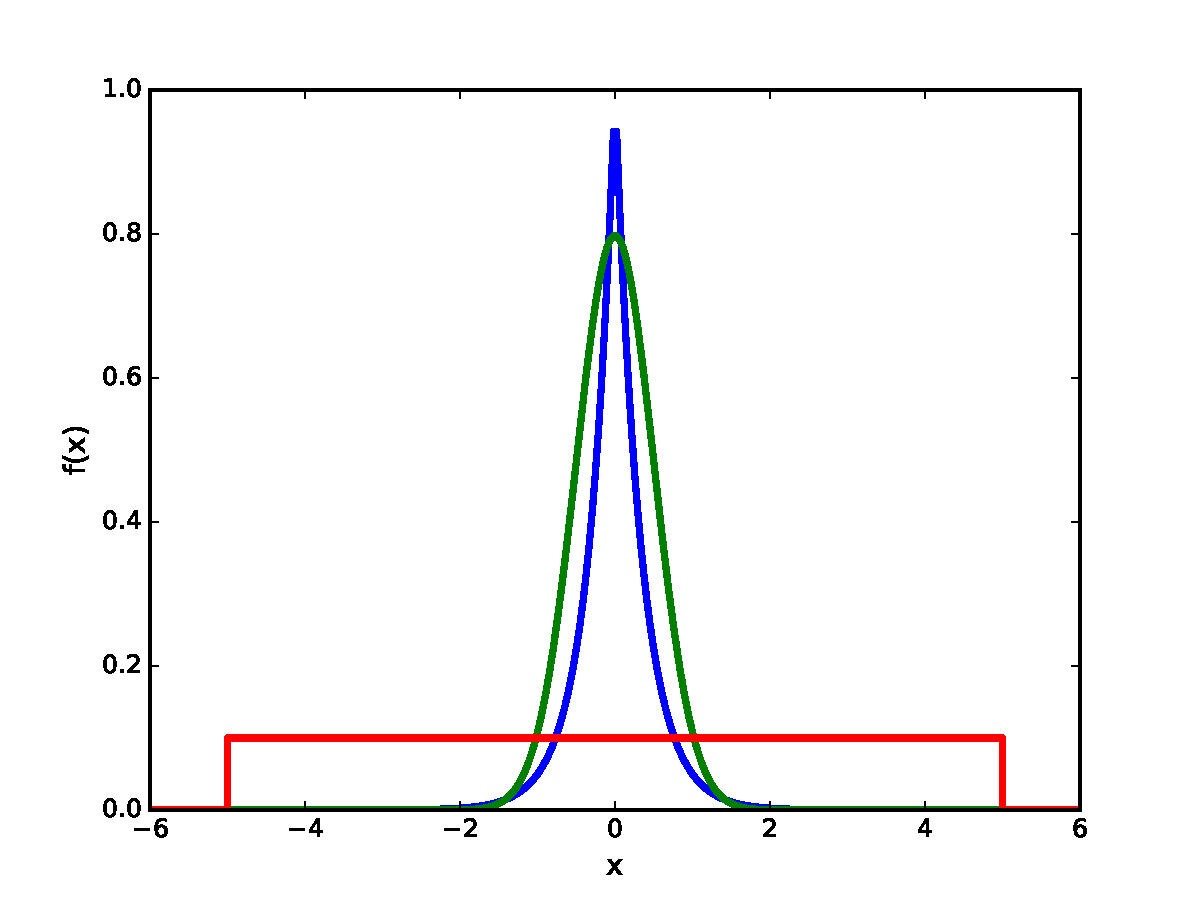
\includegraphics[width=\textwidth]{importanceSampling}
		\caption{A simple importance sampling example (see equation~\eqref{eqn:simpleIS}).  The integrand, $f(x)$, is shown in blue,
		the importance sampling distribution is shown in green and, for comparison, the uniform probability density function used
		in the na\"ive case of no importance sampling is also shown (in red).}
		\label{fig:simpleIS}
  	\end{figure}

  	Tab.~\ref{tab:simpleIS} clearly shows the value of an importance sampling approach convergences to the correct result
  	much faster than when we sample uniformly. Of course this tactic relies on us having some prior knowledge of the behaviour of our
  	integrand in order to select the correct probability density function to use which, in more complicated examples is not always
  	possible\footnote{More novel approaches whereby the sampling distribution is modified to improve convergence as the Monte-Carlo
  	iterations are calculated, such as the \texttt{VEGAS} algorithm,
  	exist but they will not be discussed here.}. A more realistic, and relevant, example of importance sampling comes from the
  	cross-section for the production of a $Z^0$ boson in association with dijets.  The matrix element squared for such a process
  	will have following form upon factoring out the $Z^0$ propagator squared:

  	\begin{equation}
  		|\mathcal{M}_{Z^0+jj}|^2 \sim \left|\frac{1}{p_Z^2 - M_Z + i\Gamma_ZM_Z}\right|^2\times f(\text{QCD, EW})\times g(\text{Kinematic}),
  		\label{eqn:schematicZ}
  	\end{equation}

  	where $p_Z$ is the momentum carried by the $Z^0$ boson, $M_Z$ is its mass, $\Gamma_Z$ is its width and $f(\text{QCD, EW})$ will
  	contain all of the coupling information and $g(\text{Kinematic})$ encodes the remainder of the matrix element.  When using a
  	Monte-Carlo approach to generate events of this kind we can use the schematic form of eqn.~\eqref{eqn:schematicZ} to \emph{a priori} select
  	an appropriate probability density function to sample from.  Fig.~\eqref{fig:breitWigner} shows the squared $Z^0$ propagator.
  	Obvious comparisons with fig.~\eqref{fig:simpleIS} can be drawn in the sense that were we to generate events with a uniform spread
  	of values for $p_Z^2$ we would end with a very slow rate of convergence by oversampling areas where the integrand is very small and slowly varying.

	\begin{figure}[htp]
		\centering
		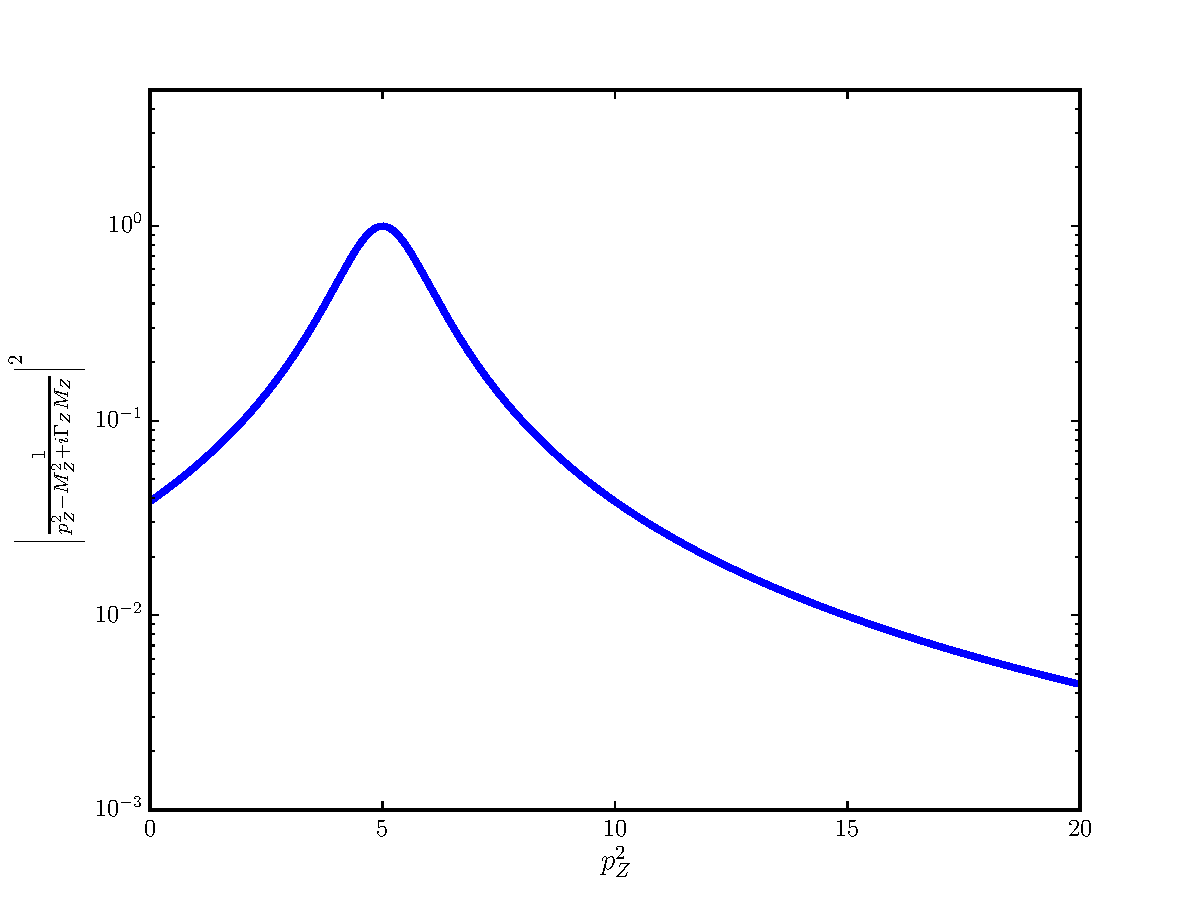
\includegraphics[width=0.8\textwidth, height=0.6\textwidth]{breitWigner}
		\caption{The absolute value squared of the $Z^0$ propagator for a range of values of the invariant mass squared of the
		$Z^0$, $p_Z^2$.  We see that, as expected, it is strongly peaked at the $Z^0$ mass and, as such, is an ideal
		candidate for using importance sampling.}
		\label{fig:breitWigner}
  	\end{figure}

	\begin{figure}[htp]
		\centering
		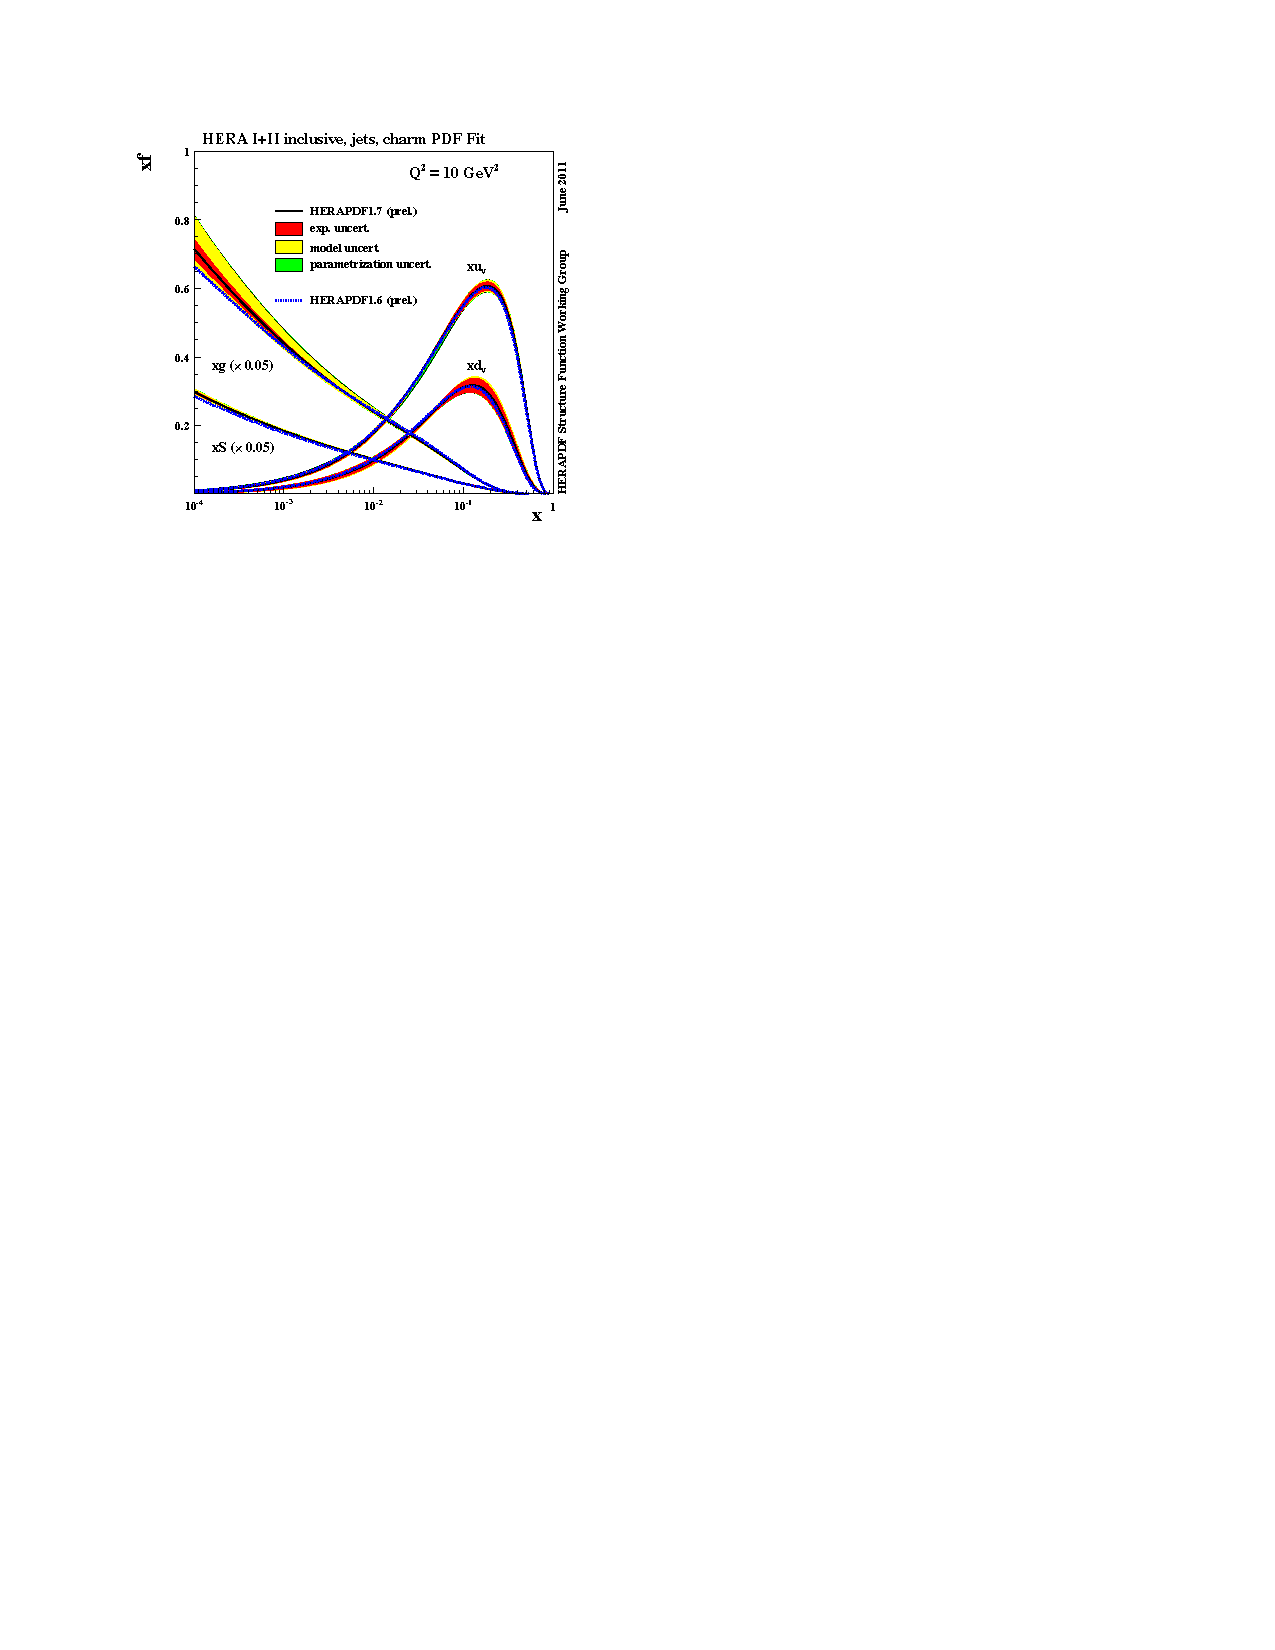
\includegraphics[width=0.8\textwidth, height=0.6\textwidth]{HERAFit}
		\caption{Recent parton distribution function fits from the HERA experiment.  The observed variation in $f(x_{a/b}, Q^2)$, especially at high
		         $x_{a/b}$, can be used to reduce the variance of a Monte Carlo approach to computing eqn~\eqref{eqn:factorisation} by using an
		         importance sampling approach}
		\label{fig:heraFit}
  	\end{figure}

  	Another good example of importance sampling is found in how we sample the incoming partons in our simulations.  Simple momentum
  	conservation considerations lead us to values for the Bjorken scaling variables of our incoming partons, $x_a$ and $x_b$, and we
  	can use these to intelligently sample the available partons.  The na\"ive way to perform the sum over all possible incoming states
  	would be to uniformly choose a random number corresponding to one of the light quarks, one the light anti-quarks or to a
  	gluon\footnote{Here we mean all except the top and anti-top.  The parton density functions for these are not available
  	and, even if they were, they would be small enough that we could safely ignore their contribution to cross-sections.}.  We can,
  	however, do better than this by using what we know about how the parton density functions vary with $x_{a/b}$ - fig.~\eqref{fig:heraFit}
  	shows this behaviour as measured by the HERA experiment.  By choosing to randomly sample then incoming parton types according to the relative values
  	for the parton density functions we can, once again, reduce the variance of our numerical integrations as much as possible.

  	As one final case study of importance sampling at work we shown a comparison of data from the CMS collaboration to two Monte Carlo
  	generators; \HEJ and \texttt{MadGraph} (v5)~\cite{CMS:2014vtk}.  The study focused on double-differential Drell-Yan production in
  	association with 0-, 1- and 2-jet final states (though here we will only discuss the 2-jet final state for reasons which will
  	be explained in later sections).  In \HEJ the production of the Drell-Yan decay products via a $Z^0$ boson or an off-shell photon
  	is implemented by using exactly the importance sampling scheme shown in eqn.~\eqref{eqn:schematicZ} and fig.~\eqref{fig:breitWigner} -
  	that is we focus our matrix element evaluations predominantly around the $Z^0$ mass peak. Fig.~\eqref{fig:HEJ_CMS2} shows the
  	comparisons to data for the three di-lepton invariant mass ranges studied.  Fig.~\eqref{fig:HEJ_CMS2_1}. shows the distribution
  	in terms of the absolute value of the rapidity between the reconstructed di-lepton pair and the leading jet in $p_\perp$ for a di-lepton
  	invariant mass of between 60 and 120~GeV (i.e. centered on the $Z^0$ peak).  We see that both \texttt{MadGraph} and \HEJ give a good
  	description of data across the full range of rapidity gaps.  Figs.~\eqref{fig:HEJ_CMS2_2} and ~\eqref{fig:HEJ_CMS2_3} show the same
  	distribution but for a recombined invariant mass of between 30 and 60~GeV - fig.~\eqref{fig:HEJ_CMS2_2} was generated using the standard
  	importance sampling (which is clearly designed for here) while fig.~\eqref{fig:HEJ_CMS2_3} was generated using a modified importance
  	sampling approach which is more suitable for probing the low mass end of the Breit-Wigner distribution.  Clearly using an intelligently
  	chosen importance sampling scheme makes a big difference to the results - since, although the integrals are formally equal, when we
  	come to perform the Monte Carlo integration we must use what computational resources we have to focus on the regions which contribute
  	most to the integral.  Figs.~\eqref{fig:HEJ_CMS2_4} and ~\eqref{fig:HEJ_CMS2_5} show the same distribution now for a di-lepton invariant
  	mass of between 120 and 1500~GeV, once again fig.~\eqref{fig:HEJ_CMS2_4} was calculated with the default importance sampling whereas
  	fig.~\eqref{fig:HEJ_CMS2_5} used a modified scheme.  The same behaviour can be seen with the na\"ive sampling describing the data
  	poorly.

	\begin{figure}[h]
		\centering
		\begin{subfigure}[b]{0.65\textwidth}
		  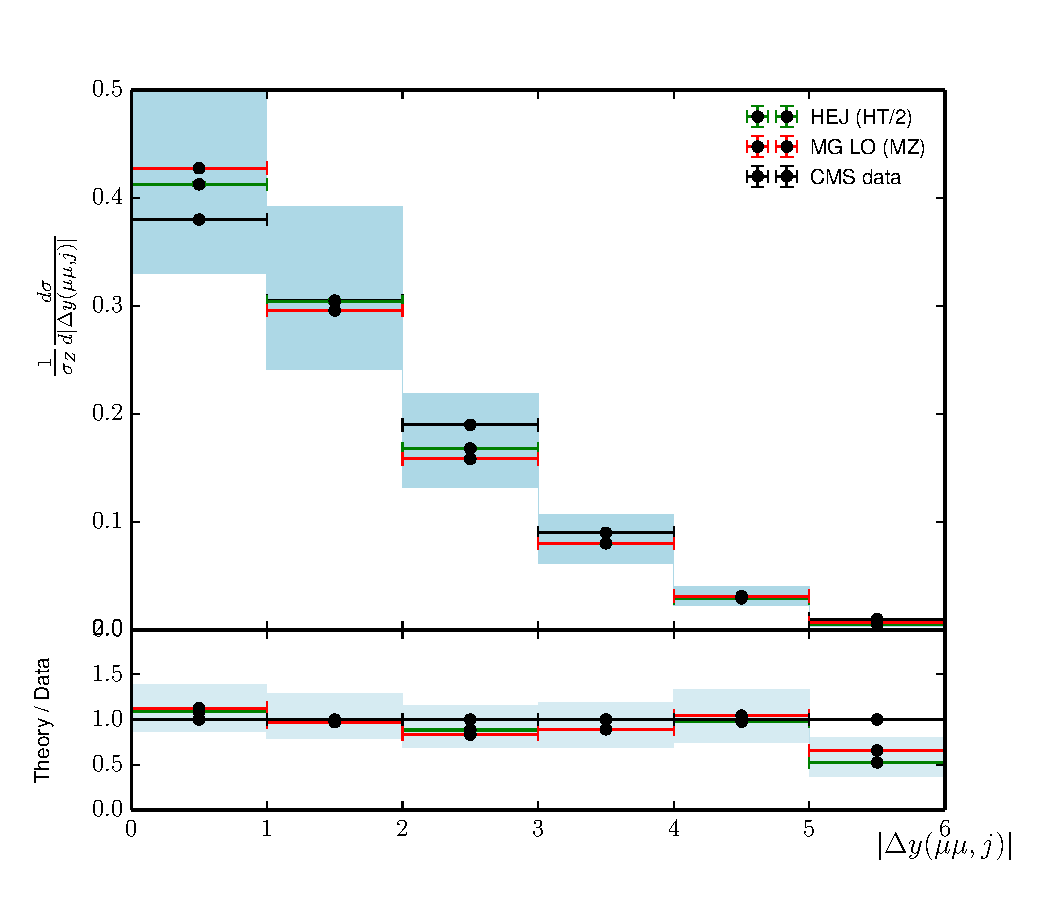
\includegraphics[width=\textwidth]{CMS2_Z_M60_120H}
		  \caption{}
		  \label{fig:HEJ_CMS2_1}
		\end{subfigure}
		\begin{subfigure}[b]{0.45\textwidth}
		  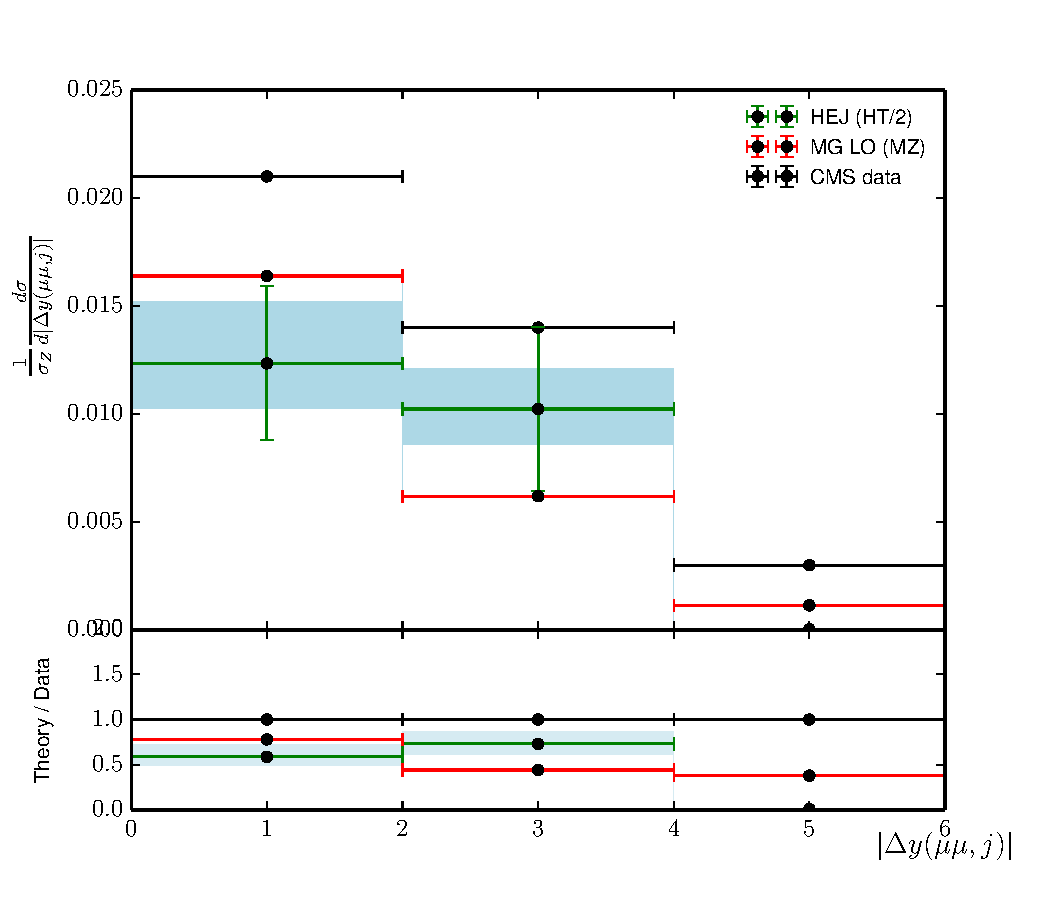
\includegraphics[width=\textwidth]{CMS2_Z_M30_60H}
		  \caption{}
		  \label{fig:HEJ_CMS2_2}
		\end{subfigure}
		~
		\begin{subfigure}[b]{0.45\textwidth}
		  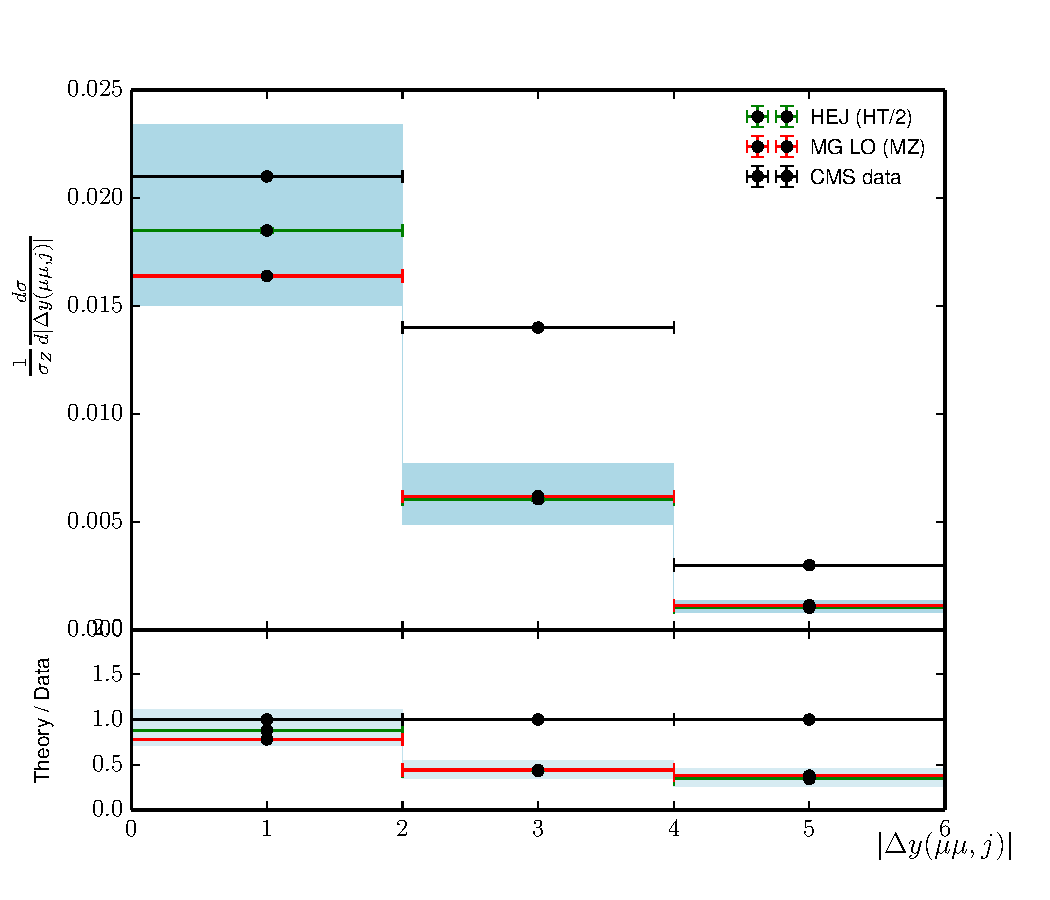
\includegraphics[width=\textwidth]{CMS2_F_M30_60H}
		  \caption{}
		  \label{fig:HEJ_CMS2_3}
		\end{subfigure}

		\begin{subfigure}[b]{0.45\textwidth}
		  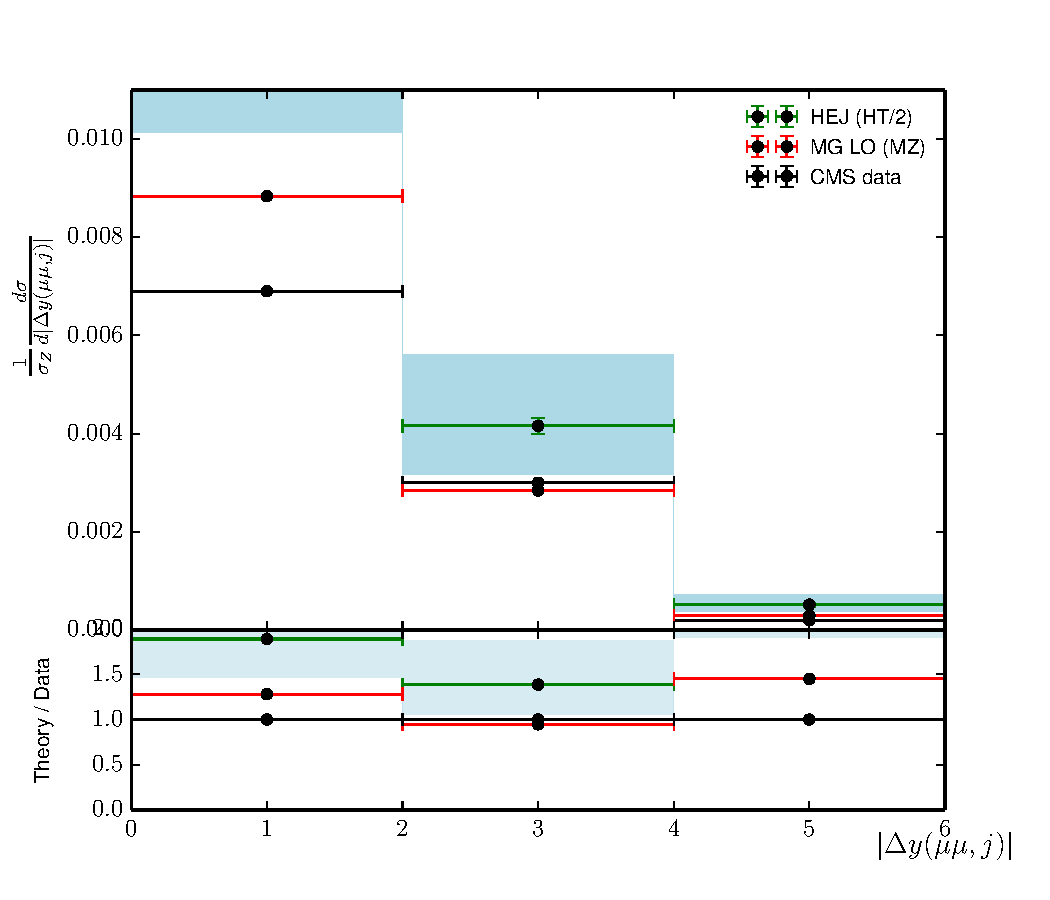
\includegraphics[width=\textwidth]{CMS2_Z_M120_1500H}
		  \caption{}
		  \label{fig:HEJ_CMS2_4}
		\end{subfigure}
		~
		\begin{subfigure}[b]{0.45\textwidth}
		  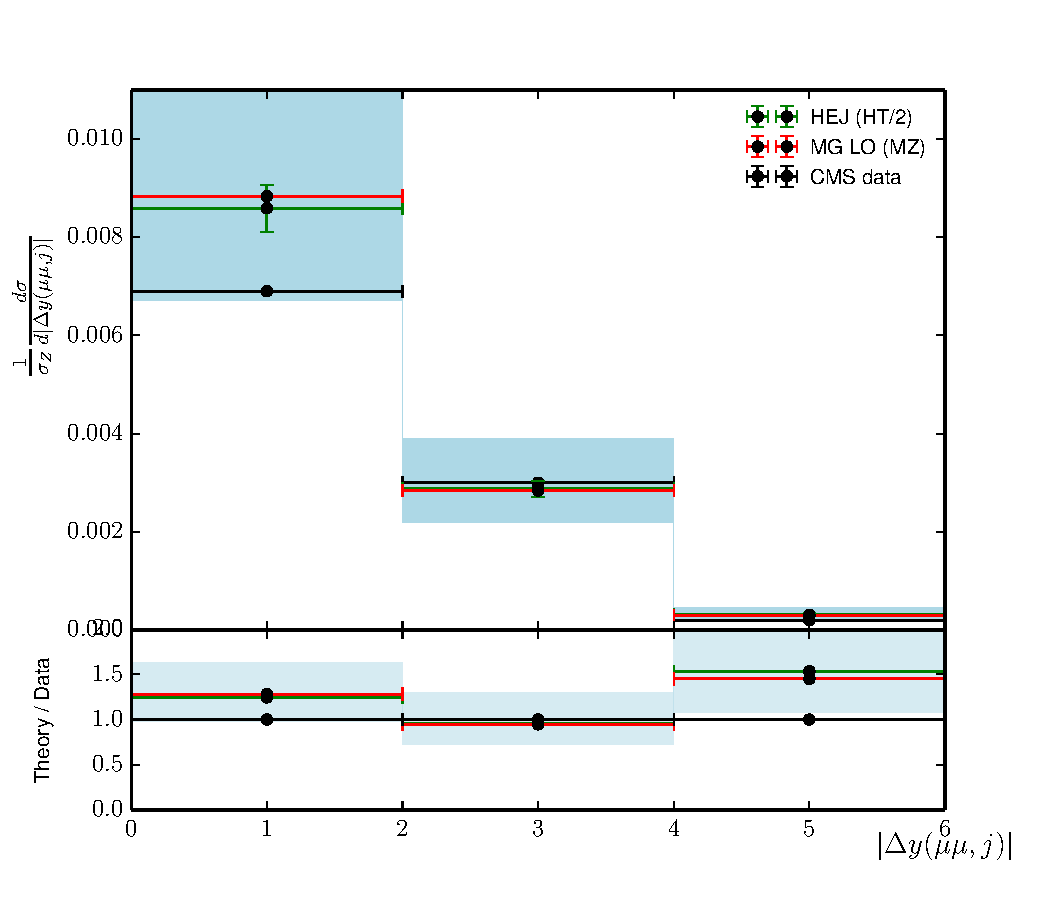
\includegraphics[width=\textwidth]{CMS2_H_M120_1500H}
		  \caption{}
		  \label{fig:HEJ_CMS2_5}
		\end{subfigure}
		\label{fig:HEJ_CMS2}
		\caption{}
	\end{figure}

	% General theory
\chapter{Monte Carlo Techniques}
\label{cha:MC}

\section{One Dimensional Monte Carlo}
\label{sec:MCOneD}

\section{Higher Dimensional Monte Carlo}
\label{sec:MCND}

\section{Variation Reduction Techniques}
\label{sec:VarReduction}

	% General theory
\chapter{High Energy QCD}
\label{chap:HEQCD}

	{\color{red}
	Stuff for this section
	\begin{itemize}
		\item Tiny bit about cuts S matrix to Optical theorem,
		\item NLO calculation of leading part of gg->gg (explain sub-leading bits) - do this bit using cuts,
		\item Extra real corrections and writing these as contractions of currents,
		\item A bit on HE phase-space integrals?
	\end{itemize}
	}

	In this chapter we look in detail at the `High Energy' limit of QCD.  We begin by defining this limit and
	looking at how basic $2\rightarrow2$ scattering behaves at leading order and next-to-leading order in
	$\alpha_s$.

	\section{The `High Energy' limit}
		\label{sub:HElimit}

		The `High Energy' limit of QCD, also referred to as the Multi-Regge Kinematic (MRK) limit is
		defined in terms of the kinematics of the final state.  We require a \emph{strong rapidity ordering}
		of all outgoing radiation as well as all the emissions having \emph{similar transverse momenta}.
		Mathematically this is:

		\begin{equation}
			y_1\gg y_2\gg\cdots\gg\\y_n \text{ and } |p_{\perp1}| \approx |p_{\perp2}| \approx\cdots\approx|p_{\perp(n-1)}|,
			\label{eqn:MRK}
		\end{equation}

  		where we define the rapidity of a final states particle as

		\begin{equation}
			y = \half\frac{E+p_z}{E-p_z}
			\label{eqn:rap}
		\end{equation}

		where $E$ is the energy of particle and $p_z$ it the $z$ component of its momentum. We can
		state the of the criteria in eq. \eqref{eqn:MRK} equivalently as $s_{ij}\rightarrow\infty$ where
		$s_{ij} = (p_i + p_j)^2$.  We sometimes instead use the pseudo-rapidity, $\eta$, which is
		simply related to the angle of the outgoing state to the beam, $\theta$:

		\begin{equation}
			\eta = -\ln\tan\frac{\theta}{2}.
			\label{eqn:prap}
		\end{equation}

		For massless states eqs. \eqref{eqn:rap} and \eqref{eqn:prap} are equivalent.

	\section{Mandelstam Variables in the High Energy Limit}
		\label{sub:MandelstamVariables}

		The $2\rightarrow 2$ QCD scattering amplitudes can be expressed in terms of the well-known Mandestam
		variables $s$, $t$ and $u$.  Which, in terms of the momenta in the process, are given by:

		\begin{subequations}
			\begin{equation}
				s = (p_1 + p_2)^2
			\end{equation}
			\begin{equation}
				t = (p_1 - p_2)^2
			\end{equation}
			\begin{equation}
				u = (p_2 - p_3)^3
			\end{equation}
			\label{eqn:mandel}
		\end{subequations}

		When working in the high energy limit it is convenient to re-express these in terms of the
		perpendicular momentum of the outgoing partons, $p_\perp$, and the difference in rapidity
		between the two final state partons, $\Delta y$.  If we parametrise our outgoing states as

		\begin{align}
		\begin{split}
			p_1 = p_{\perp1}\big(\cosh (y_1), \cos(\phi_1), \sin(\phi_1), \sinh (y_1)\big),\\
			p_2 = p_{\perp2}\big(\cosh (y_2), \cos(\phi_2), \sin(\phi_2), \sinh (y_2)\big),
		\end{split}
		\end{align}

		then we can express eqs. \eqref{eqn:mandel} as follows

		\begin{subequations}
			\begin{equation}
				s = 4p_\perp^2 \cosh^2\frac{\Delta y}{2},
			\end{equation}
			\begin{equation}
				t = -2p_\perp^2 \cosh\frac{\Delta y}{2}e^{-\frac{\Delta y}{2}},
			\end{equation}
			\begin{equation}
				u = -2p_\perp^2 \cosh\frac{\Delta y}{2}e^{\frac{\Delta y}{2}}.
			\end{equation}
		\end{subequations}

		In the limit of hard jets well separated in rapidity, i.e. $\Delta y\rightarrow\infty$,
		these are well approximated by

		\begin{subequations}
			\begin{equation}
				s = p_\perp^2 e^{\Delta y}
			\end{equation}
			\begin{equation}
				t = -p_\perp^2
			\end{equation}
			\begin{equation}
				u = -p_\perp^2 e^{\Delta y}
			\end{equation}
		\end{subequations}

		From this it is clear that the `hard, wide-angle jet' limit is equivalent to the High Energy
		limit since as $\Delta y$ grows large $s$ will grow exponentially while $t$ will stay fixed.
		Rearranging for $\Delta y$ in the above equations yields:

		\begin{equation}
			\Delta y = \ln \left(\frac{s}{-t}\right).
			\label{eqn:largeLogs}
		\end{equation}

		This is a useful result because it relates the simple kinematics of an event to a (potentially)
		large logarithm.  It is already naively clear from eq. \eqref{eqn:largeLogs} that a final state
		with large rapidity gaps could require a more careful inspection than the fixed-order approach
		discussed in section \ref{sec:pqcdAndResum}.

	\section{$qQ$-scattering at High Energy}
		\label{sec:qQScat}

		Here we begin with the simplest example; the case of $qQ\rightarrow qQ$ for all negative helicity partons
		\footnote{where the capital $Q$ implies it is a different flavour to $q$ - and hence we need not consider the crossed
		diagrams which would contribute if they were the same flavour}. There is only one diagram which contributes shown
		in fig. (\ref{fig:TwoToTwo}).  Using the Feynman rules detailed in section \ref{sec:partonicCrossSection} we can
		write the matrix element as:

		\begin{align}
			i\mathcal{M}_{q^-Q^-\rightarrow q^-Q^-}^{\text{LO}} &= ig_s^2T^d_{1a}T^d_{2b}\frac{\overline{u}^-(p_1)\gamma^\mu
			  u^-(p_a)\overline{u}^-(p_2)\gamma_\mu u^-(p_b)}{t}\\
			  &= ig_s^2T^d_{1a}T^d_{2b}\frac{\bk{1}{\mu}{a}\cdot\bk{2}{\mu}{b}}{t},
			  \label{eqn:similarBrackets}
		\end{align}

		where $t = (p_a - p_1)^2$ and we have used the shorthand $\overline{u}^-(p_i)\gamma^\mu u^-(p_j) = \bk{i}{\mu}{j}$ in the second line.
		Writing the contraction of these two `current' terms in terms of light-cone coordinates we have:

		\begin{equation}
			i\mathcal{M}_{q^-Q^-\rightarrow q^-Q^-}^{\text{LO}} = ig_s^2T^d_{1a}T^d_{2b}\frac{2\sqrt{p_a^-p_b^+}}{t}
			\left(\sqrt{p_1^+p_2^-}e^{i\phi_2} + \sqrt{p_1^-p_2^+}e^{i\phi_1}\right),
			\label{eqn:qQ2qQ}
		\end{equation}

		where $e^{i\phi_i} = \frac{p_{\perp i}}{|p_{\perp i}|}$.  We now approximate the kinematics in such a way that we may write
		eq. \eqref{eqn:qQ2qQ} in a `factorised' form once again.  Specifically we consider that the scattering can be thought
		of as two partons glancing off one another.  That is, we assume that $p_1^+\ll p_1^-$ and $p_2^-\ll p_2^+$.  We can further
		assume that $p_1^-\approx p_a^-$ and $p_2^-\approx p_b^-$ and with this we see that \eqref{eqn:qQ2qQ} becomes:

		\begin{equation}
			i\mathcal{M}_{q^-Q^-\rightarrow q^-Q^-}^{\text{LO}} = \frac{2s}{t}\left(g_sT^d_{1a}e^{i\phi_1}\right)\left(-ig_sT^d_{2b}\right),
			\label{eqn:reggeTraj}
		\end{equation}

		which is `factorised' in the sense that each scalar term in brackets depends only on one quark line; either on the $p_{a/1}$
		line or the $p_{b/2}$ line.  We see that the amplitude for $qQ\rightarrow qQ$ is dominated by the $s$ kinematic variable.
		We can express this as:

		\begin{equation}
			\mathcal{M}_{q^-Q^-\rightarrow q^-Q^-}^{\text{LO}} \sim s^{\alpha(t)},
		\end{equation}

		which is exactly the behaviour expected when a particle exchanged in the $t$-channel has `reggeised'
		\cite{sabioThesis,DelDuca:1995hf,lipatovBook}.  $\alpha(t)$ is the Regge trajectory and is equal to
		the intrinsic spin of the state exchanged.  In our example we have have a spin-one gluon exchanged
		and accordingly we can see from eq. \eqref{eqn:reggeTraj} that $\alpha(t)=2$ for $qQ\rightarrow qQ$.

		\begin{figure}
			\begin{center}
			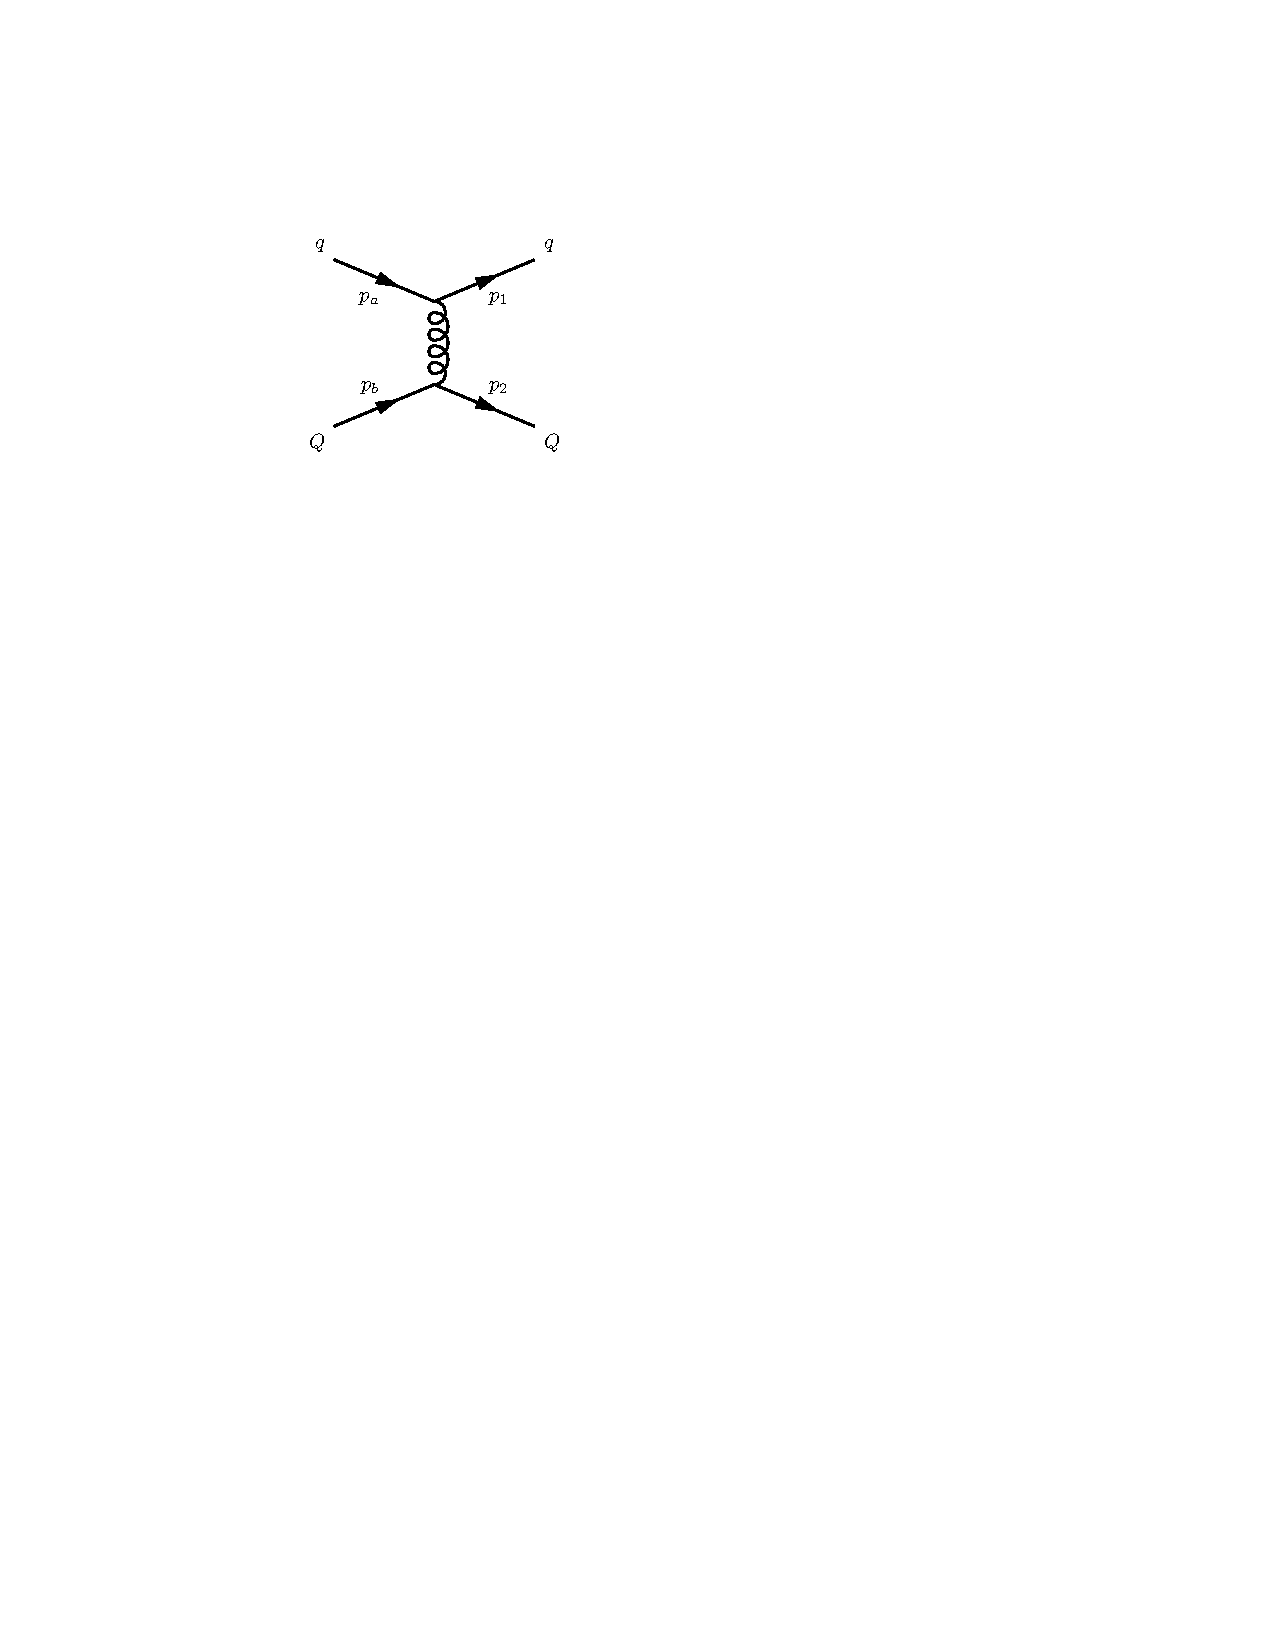
\includegraphics[width=0.35\linewidth]{TwoToTwo}
			\caption{The only diagram which contributes to $qQ\rightarrow qQ$ at leading order in $\alpha_s$.}
			\label{fig:TwoToTwo}
			\end{center}
		\end{figure}

	\section{$qg$ scattering at High Energy}

		We now with explore the more involved case of $2\rightarrow 2$ quark-gluon scattering.  At leading order this
		consists of three diagrams shown in fig. (\ref{fig:TwoToTwo}).  Here we only show the calculations
		for the helicity structure where both quark lines have fixed, and opposite, helicities.  We use
		the following gauge choice for the gluon polarisations:

		\begin{align}
		\epsilon^{+*}_{2\sigma}&=\frac{\langle b|\sigma|2\rangle}{\sqrt{2}\langle b2\rangle} & \epsilon^{-*}_{2\sigma} &= -\frac{\langle b|\sigma|2\rangle}{\sqrt{2}[b2]} \\
		\epsilon^{+}_{b\sigma}&=-\frac{\langle b|\sigma|2\rangle}{\sqrt{2}[2b]} & \epsilon^{-*}_{2\sigma} &= -\frac{\langle b|\sigma|2\rangle}{\sqrt{2}\langle 2b\rangle}
		\end{align}

		For simplicity we alter the notation slightly and choose to treat everything as having negative helicity.
		To describe positive helicities we can use the transposition property of spinor-helicity brackets discussed
		from section \ref{sec:SpinorHelicity}.

		\begin{figure}[h]
			\centering
			\begin{subfigure}[b]{0.3\textwidth}
				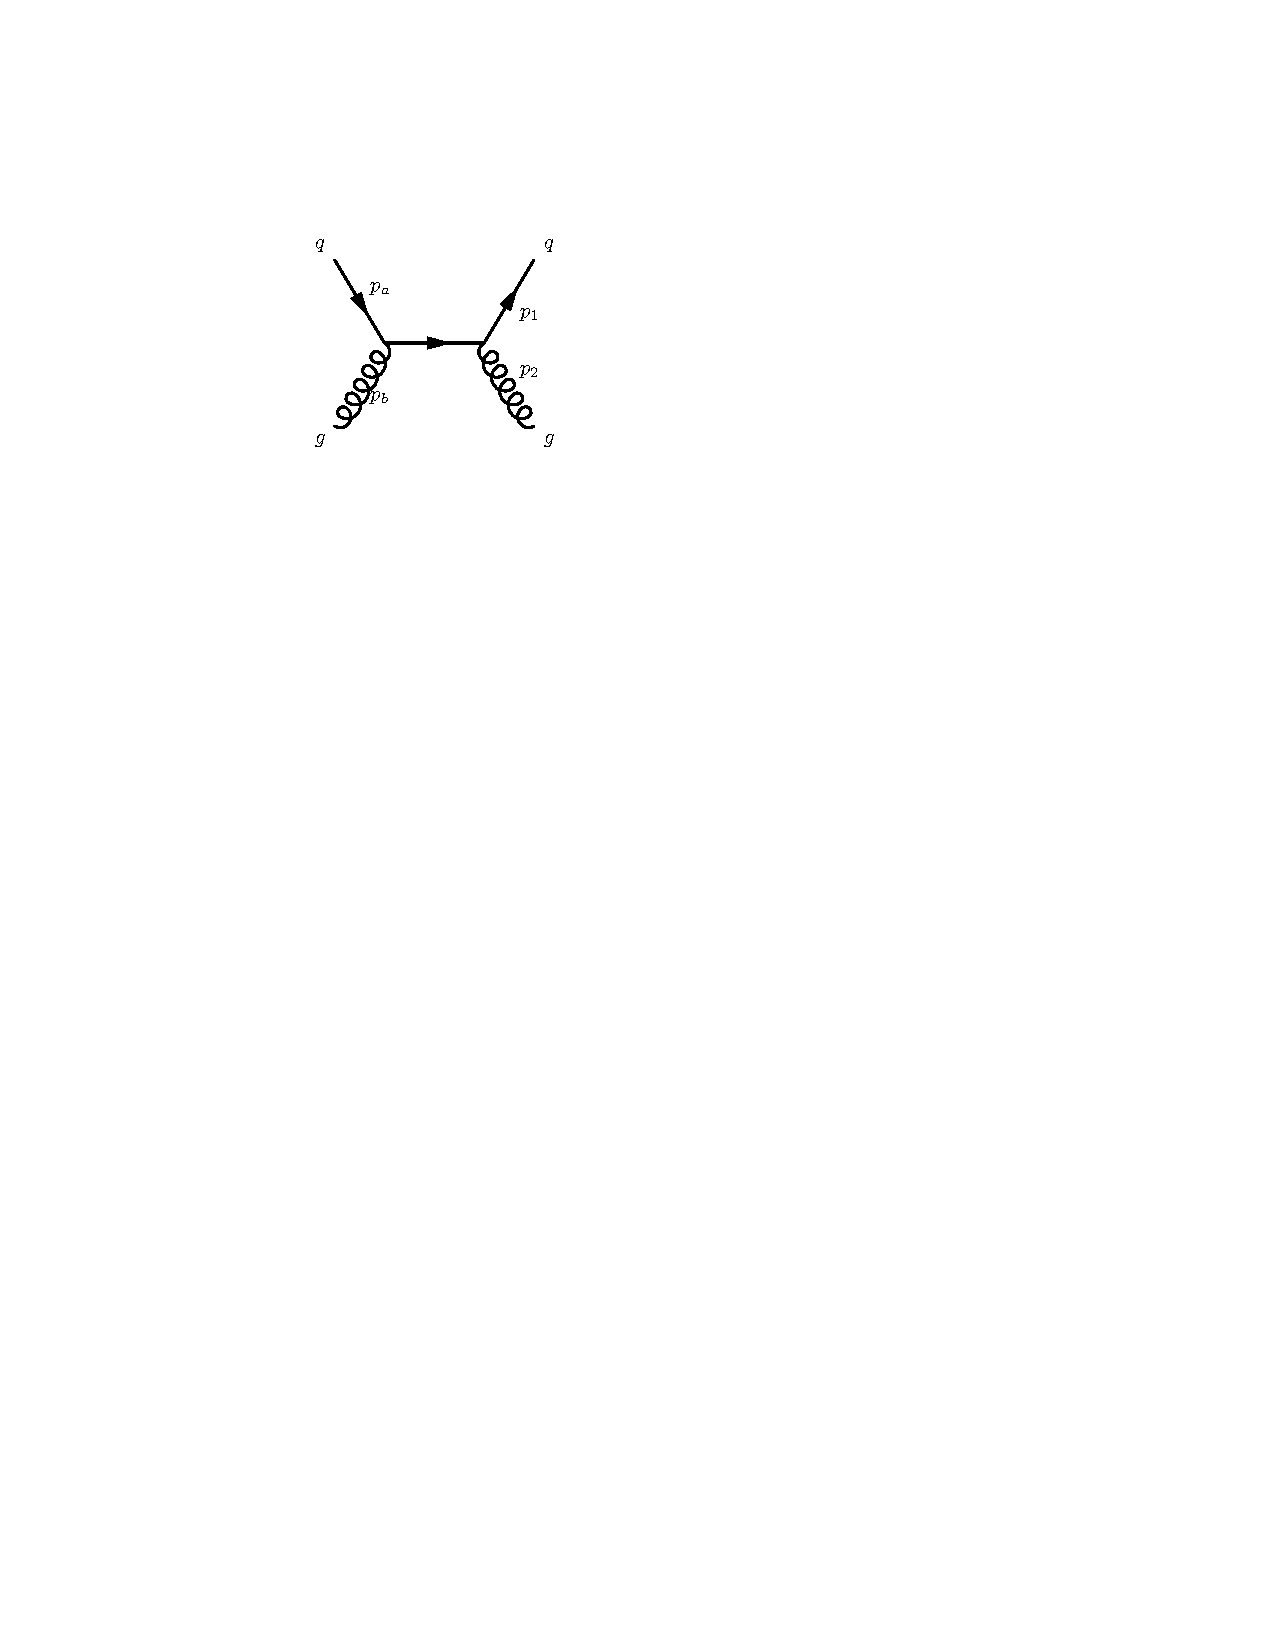
\includegraphics[width=\textwidth]{qg2qg-s}
				\caption{}
				\label{fig:qg2qg-s}
			\end{subfigure}

			\begin{subfigure}[b]{0.3\textwidth}
				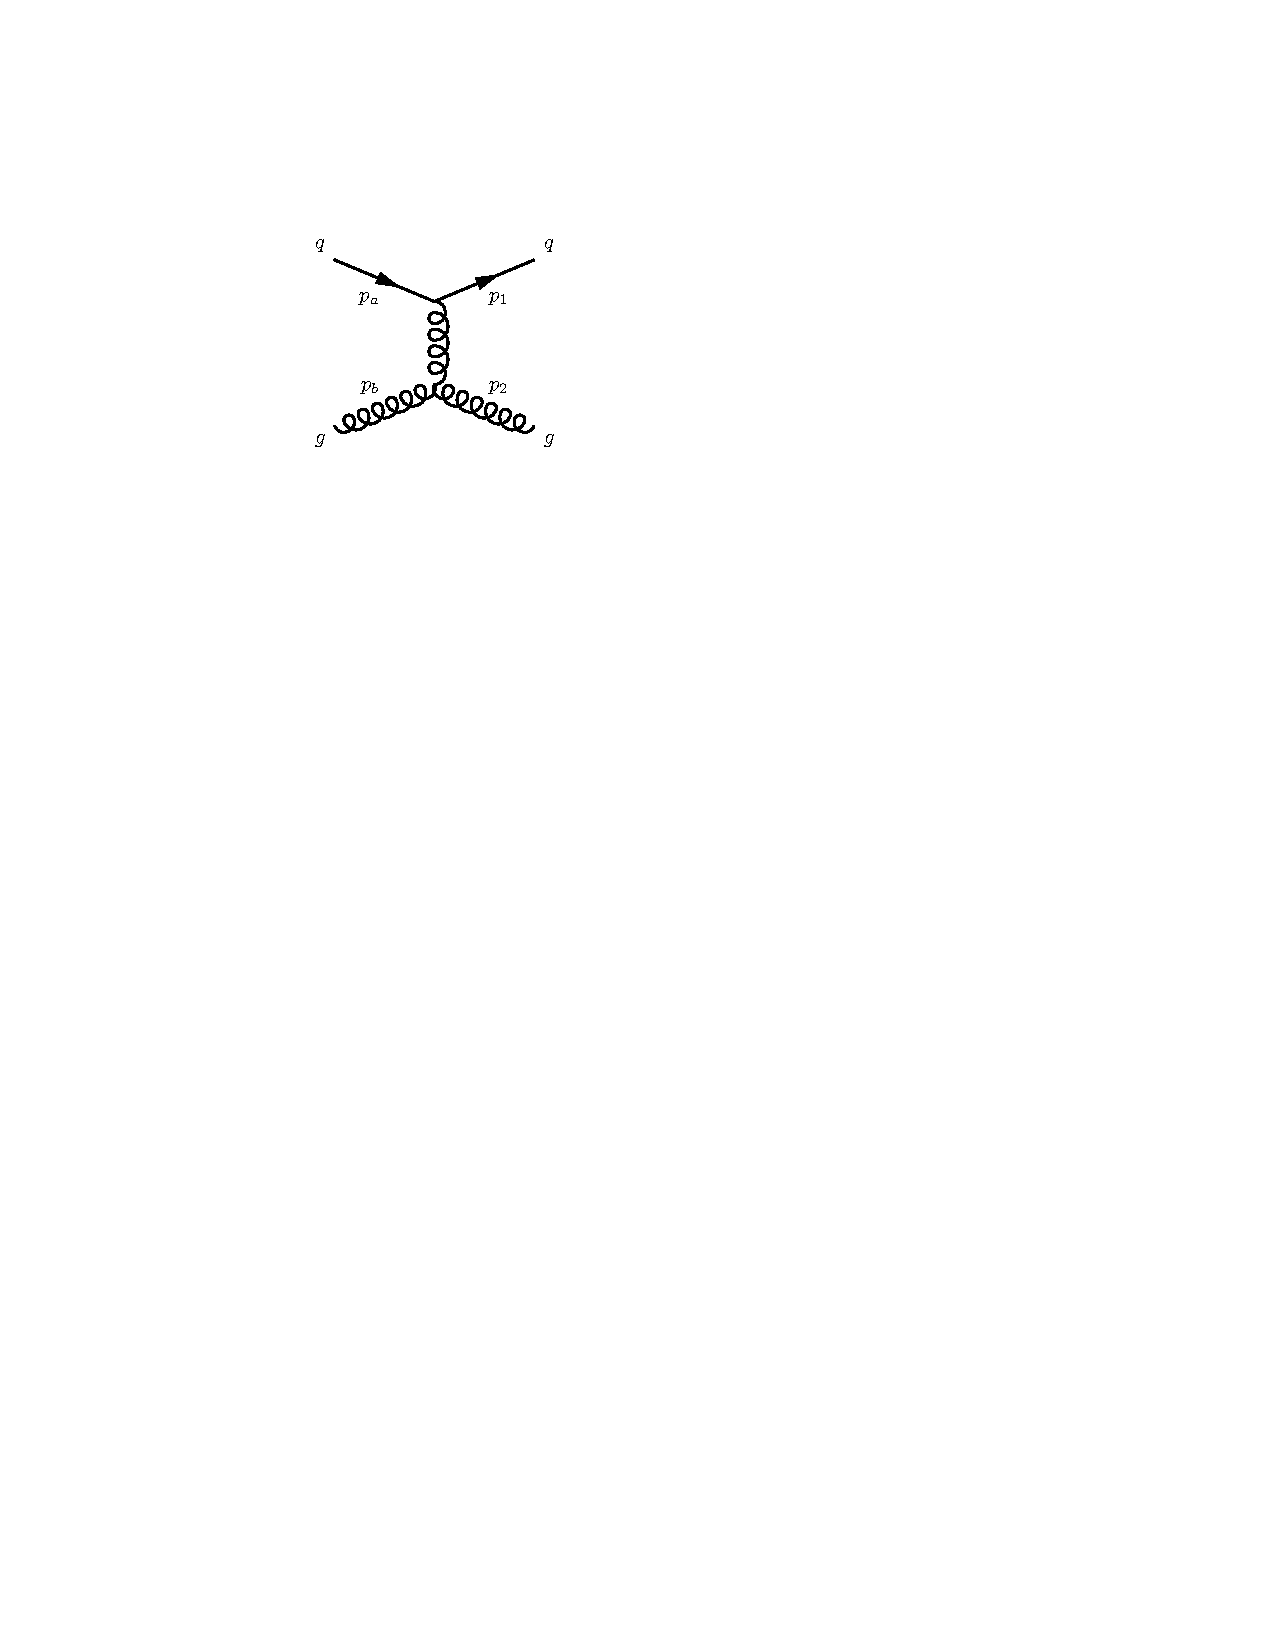
\includegraphics[width=\textwidth]{qg2qg-t}
				\caption{}
				\label{fig:qg2qg-t}
			\end{subfigure}
			~
			\begin{subfigure}[b]{0.3\textwidth}
				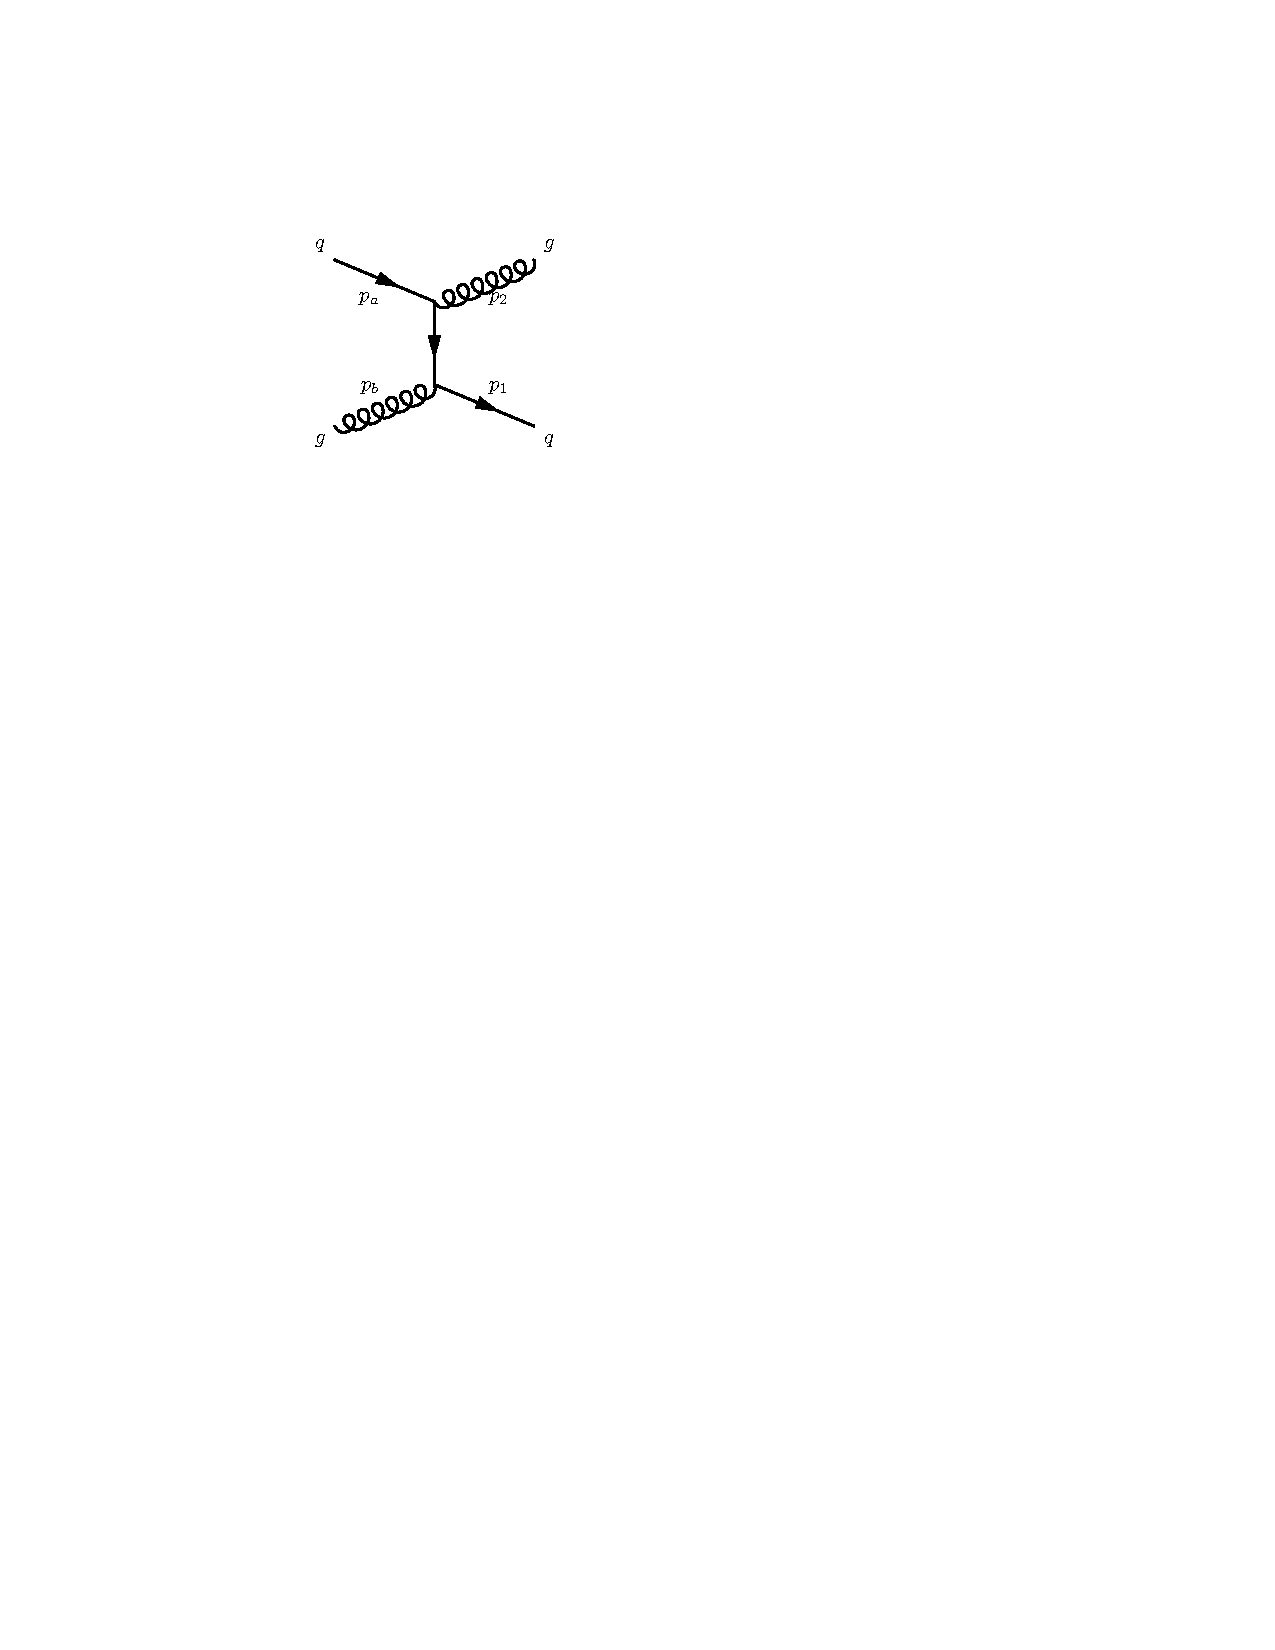
\includegraphics[width=\textwidth]{qg2qg-u}
				\caption{}
				\label{fig:qg2qg-u}
			\end{subfigure}
			\caption{The $s$, $t$ and $u$ channel diagrams contributing to $qg\rightarrow qg$ at leading
			         order in $\alpha_s$ in figures (\ref{fig:qg2qg-s}), (\ref{fig:qg2qg-t}) and (\ref{fig:qg2qg-u})
			         respectively.}
		\end{figure}

		\subsection{$s$-channel}

			The matrix element for the $s$-diagram, shown in fig. \eqref{fig:qg2qg-s}, is:

			\begin{align}
				\mathcal{M}_{qg\rightarrow qg, s}^{\text{LO}}=&\overline{u}^-(p_1)\left(-\frac{ig_s}{2}\gamma^\mu\right)\epsilon_\mu^{*+}(p_2)
					\frac{i(\slashed q+m)}{q^2-m^2}\left(-\frac{ig_s}{2}\gamma^\nu\right)\epsilon^+_\nu(p_b)u^-(p_a), \\
				=&-\frac{g^2_s}{4q^2}\epsilon^{*+}_{2\mu}\epsilon^+_{b\nu}\overline{u}^-_1\gamma^\mu\slashed q\gamma^\nu u^-_a,
			\end{align}

			where we have used $q\gg mc$ for the high energy case.  The propagator has momentum $q=p_a+p_b=p_1+p_2$ and therefore:

			\begin{align}
				\mathcal{M}_{qg\rightarrow qg, s}^{\text{LO}}=&-\frac{g^2_s}{4q^2}\frac{\langle{b}|\mu|2\rangle}{\sqrt{2}\langle{b2\rangle}}
				\frac{\langle{b}|\nu|2\rangle}{\sqrt{2}[2b]}\overline{u}^-_1\gamma^\mu(\slashed{p}_a+\slashed{p}_b)\gamma^\nu u^-_a,\\
				=&-\frac{g^2_s}{8q^2s_{2b}}\langle{b}|\mu|2\rangle\langle{b}|\nu|2\rangle
				\left(\overline{u}^-_1\gamma^\mu\gamma^\sigma\gamma^\nu u^-_ap_{a\sigma}+
				\overline{u}^-_1\gamma^\mu\gamma^\sigma\gamma^\nu u^-_ap_{b\sigma}\right).
			\end{align}

			The gamma matrices satisfy the Clifford algebra, $\{\gamma^\mu, \gamma^\nu\}=2g^{\mu\nu}$ and so we may write:

			\begin{equation}
				\overline{u}^-_1\gamma^\mu\gamma^\sigma\gamma^\nu u^-_ap_{a\sigma}=
				\overline{u}^-_1\gamma^\mu\gamma^\nu\gamma^\sigma u^-_ap_{a\sigma} -
				2\overline{u}^-_1\gamma^\mu g^{\sigma\nu}u^-_ap_{a\sigma}
			\end{equation}

			but in the High Energy limit the Dirac equation is $\slashed{p}_au^-_a=0$:

			\begin{equation}
				\mathcal{M}_{qg\rightarrow qg, s}^{\text{LO}}=-\frac{g^2_s}{8q^2s_{2b}}\langle{b}|\mu|2\rangle\langle{b}|\nu|2\rangle
				\left(-2\overline{u}^-_1\gamma^\mu u^-_ap_{a}^\sigma+\overline{u}^-_1\gamma^\mu\gamma^\sigma\gamma^\nu u^-_ap_{b\sigma}\right)
			\end{equation}

			For the second term we must use the following identity:

			\begin{equation}
				\gamma^\mu\gamma^\sigma\gamma^\mu=g^{\mu\sigma}\gamma^\nu + g^{\sigma\nu}\gamma^\mu
				- g^{\mu\nu}\gamma^\sigma - i\epsilon^{\rho\mu\sigma\nu}\gamma_\rho\gamma^5,
			\end{equation}

			where $\epsilon^{\rho\mu\sigma\nu}$ is the four dimensional totally antisymmetric symbol:

			\begin{align}
			\begin{split}
				\mathcal{M}_{qg\rightarrow qg, s}^{\text{LO}} = &-\frac{g^2_s}{8q^2s_{2b}} \bk{b}{\mu}{2} \bk{b}{\nu}{2} \Big(\bk{1}{\mu}{a} p_a^\nu \\
				&+ p_{b\sigma}\overline{u}^-_1(g^{\mu\sigma}\gamma^\nu + g^{\sigma\nu}\gamma^\mu
				- g^{\mu\nu}\gamma^\sigma - i\epsilon^{\rho\mu\sigma\nu}\gamma_\rho\gamma^5)\Big)\\
				= &-\frac{g^2_s}{8q^2s_{2b}}\langle{b}|\mu|2\rangle\langle{b}|\nu|2\rangle
				\Big(\langle 1|\mu|a\rangle \langle a|\nu|a\rangle + \langle b|\mu|b\rangle
				\langle 1|\nu|a\rangle \\
				&+ \langle b|\sigma|b\rangle\langle1|\sigma|a\rangle
				g^{\mu\nu} - i\langle b|\sigma|b\rangle\langle 1|\epsilon^{\rho\mu\sigma\nu}\gamma_\rho\gamma^5|a\rangle\Big).
			\end{split}
			\end{align}

			The second, third and fourth terms are zero because, for example:

			\begin{equation}
				\langle b|\mu|2\rangle\langle b|\mu|b\rangle = 2[2b]\langle b b\rangle = 0,
			\end{equation}

			and therefore

			\begin{equation}
				\mathcal{M}_{qg\rightarrow qg, s}^{\text{LO}}=-\frac{g^2_s}{4q^2s_{2b}}[2a]\langle ab\rangle\langle{b}|\mu|2\rangle\langle{1}|\mu|a\rangle
			\end{equation}

			Using $q^2=s_{ab}=\langle ab\rangle[ba]$ and $s_{2b}=\langle2b\rangle[b2]$ we have:

			\begin{equation}
			\mathcal{M}_{qg\rightarrow qg, s}^{\text{LO}}=-\frac{g^2_s}{4}\frac{[2a]\langle ab\rangle}{\langle ab\rangle[ba]
			\langle2b\rangle[b2]}\langle{b}|\mu|2\rangle\langle{1}|\mu|a\rangle.
			\end{equation}

			Now we must calculate the spinor products.  We use the conventions for spinors outlined in the
			previous chapter.  For example:

			\begin{align}
				[2a] = &\overline{u}^+_2u^-_a=(u^+_2)^\dagger\gamma^0u^-_a=\left(\sqrt{p^+_2},
				\sqrt{p^-_2}\frac{p^{\perp}_2}{|p_2^\perp|}, 0, 0\right)
				\gamma^0\left( \begin {array}{c} 0\\ \noalign{\medskip}0\\ \noalign{\medskip}0\\ \noalign{\medskip}-\sqrt{p^+_a}\end {array}\right)\\
				[2a] = &\left(\sqrt{p^+_2}, \sqrt{p^-_2}\frac{p^{\perp}_2}{|p_2^\perp|}, 0, 0\right)\left( \begin {array}{c} 0\\ \noalign{\medskip}-\sqrt{p^+_a}\\
				\noalign{\medskip}0\\ \noalign{\medskip}0\end {array}\right)=-\frac{\sqrt{p_a^+p_2^-}p_2^\perp}{|p_2^\perp|}
			\end{align}

			And upon calculating the other brackets we see:

			\begin{equation}
				\mathcal{M}_{qg\rightarrow qg, s}^{\text{LO}} = -\frac{g_s^2}{4}\sqrt{\frac{p_2^-}{p_b^-}}\frac{1}{p_2^+p_b^-} \frac{p_{2\perp}^*}{|p_{2\perp}|} \bk{b}{\mu}{2} \bk{1}{\mu}{a}
			\end{equation}

			Which can be simplified slightly since $\hat{t}=s_{2b}$ to give the final result:

			\begin{equation}
				\mathcal{M}_{qg\rightarrow qg, s}^{\text{LO}}=-\frac{g_s^2}{2\hat{t}}\sqrt{\frac{p_2^-}{p_b^-}}\frac{p_{2\perp}^*}
				{|p_{2\perp}|}\langle{b}|\mu|2\rangle\langle{1}|\mu|a\rangle
				\label{eqn:s-channel}
			\end{equation}

		\subsection{$t$-channel}

			The matrix element for the $t$-diagram, shown in fig. \eqref{fig:qg2qg-t}, is:

			\begin{align}
			\begin{split}
				-i\mathcal{M}_{qg\rightarrow qg, t}^{\text{LO}} =&-\overline{u}^-_1\Bigg(-\frac{ig_s}{2}\gamma^\mu\Bigg)\Bigg(-\frac{ig_{\mu\nu}}{q^2}\Bigg)u^-_ag_sf^{\gamma\beta\delta}\\
				&\Big(g_{\sigma\nu}(p_b-q)_\rho + g_{\nu\rho}(p_b-q)_\sigma - g_{\rho\sigma}(p_b-q)_\nu)\Big)\epsilon^{\rho *}_{2+}\epsilon^{\sigma}_{b+}\\
				=&-\frac{g_s^2}{2q^2s_{2b}}\left(\overline{u}^-_1\gamma^{\nu}u^-_a\right)\left(\overline{u}^-_b\gamma^{\rho}u^-_2\right)\\
				&\left(\overline{u}^-_b\gamma^{\sigma}u^-_2\right)\left(g_{\sigma\nu}(p_b-q)_\rho + g_{\nu\rho}(p_b-q)_\sigma - g_{\rho\sigma}(p_b-q)_\nu)\right)
			\end{split}
			\end{align}

			Now using $q=p_a-p_1=p_2-p_b$:

			\begin{align*}
			i\mathcal{M}_{qg\rightarrow qg, t}^{\text{LO}} = -\frac{g_s^2}{2q^2s_{2b}}[(2p_{2\rho}-p_{b\rho})&\left(\overline{u}^-_1\gamma_{\sigma}u^-_a\right)\left(\overline{u}^-_b\gamma^{\rho}u^-_2\right)\left(\overline{u}^-_b\gamma^{\sigma}u^-_2\right)+\ldots \\
			\ldots + \hspace{2pt} (2p_{2\sigma}-p_{b\sigma})&\left(\overline{u}^-_1\gamma_{\nu}u^-_a\right)\left(\overline{u}^-_b\gamma^{\nu}u^-_2\right)\left(\overline{u}^-_b\gamma^{\sigma}u^-_2\right)-\ldots \\
			\ldots - \hspace{2pt} (p_{2\nu}\hspace{4pt}+p_{b\nu})&\left(\overline{u}^-_1\gamma^{\nu}u^-_a\right)\left(\overline{u}^-_b\gamma_{\sigma}u^-_2\right)\left(\overline{u}^-_b\gamma^{\sigma}u^-_2\right)]
			\end{align*}

			Once again in the high energy case the Dirac equation is $\slashed pu^\pm=0$ and $\overline{u}^\pm\slashed p=0$.  The first line of the above expression reads:

			\begin{equation}
			2\langle1|\sigma|a\rangle\langle b|\sigma|2\rangle\overline{u}^-_b\slashed p_2u^-_2 - \langle1|\sigma|a\rangle\langle b|\sigma|2\rangle\overline{u}^-_b\slashed p_b,
			\end{equation}

			which cancels completely.  The other two lines contain similar factors and therefore

			\begin{equation}
				\mathcal{M}_{qg\rightarrow qg, t}^{\text{LO}}=0.
				\label{eqn:t-channel}
			\end{equation}

		\subsection{$u$-channel}

			The matrix element for the $u$-diagram, shown in fig. \eqref{fig:qg2qg-t}, is:

			\begin{equation}
			\begin{split}
			-i\mathcal{A}_u &= \overline{u}^-(p_1)\left(-\frac{ig_s}{2}\gamma^\mu\right)\frac{i(\slashed q+mc)}{q^2-m^2c^2}\left(-\frac{ig_s}{2}\gamma^\nu\right)u^-(p_a)\epsilon_\mu^{*+}(p_b)\epsilon^+_\nu(p_2)\\
			\mathcal{A}_u &= \frac{g_s^2}{4q^2}\overline{u}^-_1\gamma^\mu\slashed q\gamma^\nu u^-_a\epsilon^{+*}_{b\mu}\epsilon^*_{2\nu}\\
			&= \frac{g_s^2}{8q^2s_{2b}}\langle b|\mu|2\rangle\langle b|\nu|1\rangle\overline{u}^-_1\gamma^\mu(\slashed{p}_a-\slashed{p}_2)\gamma^\nu u^-_a\\
			&= \frac{g_s^2}{8q^2s_{2b}}\langle b|\mu|2\rangle\langle b|\nu|1\rangle(\overline{u}^-_1\gamma^\mu\gamma^\sigma\gamma^\nu u^-_ap_{a\sigma} - \overline{u}^-_1\gamma^\mu\gamma^\sigma \gamma^\nu u^-_ap_{2\sigma})
			\end{split}
			\end{equation}

			Where we have used $q=p_a-p_2$.  By direct comparison with the procedure used for the $s$-channel we can see the result will be:

			\begin{equation}
			\mathcal{A}_u=\frac{g_s^2}{2\hat{t}}\sqrt{\frac{p_b^-}{p_2^-}}\frac{p_2^{\perp^*}}{|p_2^\perp|}\langle{b}|\mu|2\rangle\langle{1}|\mu|a\rangle.
			\label{eqn:u-channel}
			\end{equation}

			The total total matrix element is given by the sum of eqs. \eqref{eqn:s-channel}, \eqref{eqn:t-channel} and \eqref{eqn:u-channel} which is:

			\begin{equation}
				\mathcal{A}=\frac{g_s^2}{2}\frac{p_2^{\perp^*}}{|p_2^\perp|}\left(\sqrt{\frac{p_b^-}{p_2^-}}-\sqrt{\frac{p_2^-}{p_b^-}}\right)\frac{\langle{b}|\mu|2\rangle\langle{1}|\mu|a\rangle}{\hat{t}},
				\label{eqn:fullsum}
			\end{equation}

			Which is exactly in the form of two `currents' contracted as seen in section \ref{sec:qQScat}.  We also
			see that eqn. \eqref{eqn:fullsum} has the same spinor-helicity brackets contracted as eqn. \eqref{eqn:similarBrackets}
			and so the dominant behaviour of $gs\rightarrow qg$ in the high energy limit is $\frac{s}{t}$.\\In the High Energy
			limit we have $p_b^-\thicksim p_2^-$ and so eqn. \eqref{eqn:fullsum} could be simplified further; though we
			actually choose \emph{not} to do this so as to approximate as little as possible.  The important thing about eqn.
			\eqref{eqn:fullsum} is that this helicity structure can be described exactly at the High Energy limit by the
			exchange of a soft $t$-channel gluon.\\  All of the other helicity combinations can be calculated too we see
			they also have a pole in the $\hat t$ channel.

	\section{High Energy Jets `Currents'}
		\label{sub:currents}

		It should not come as a surprise that the $qQ\rightarrow qQ$ and $qg\rightarrow qg$ channels closely resemble
		each another since if we consider the sub-diagrams involved in the $t$-channel exchange namely the quark and
		gluon `currents' in the high energy limit we see that they themselves are similar.  The gluon emission
		current, $j_{g}^\sigma$, shown in fig. \eqref{fig:gluonCurrent} is given by

		\begin{equation}
			j_{g}^\sigma = \left((p_a+p_1)^\sigma g^{\mu\nu} + (q - p_1)^\mu g^{\nu\sigma} - (q + p_a)^\nu g^{\mu\sigma}\right)\epsilon_{a, \mu}\epsilon_{1, \nu}^*.
		\end{equation}

		In the High Energy limit we can take $p_a\sim p_1$ and therefore this becomes:

		\begin{equation}
			j_{g}^\sigma \sim \left(2p_a^\sigma g^{\mu\nu} - p_a^\mu g^{\nu\sigma} - p_1^\nu g^{\mu\sigma}\right)\epsilon_{a, \mu}\epsilon_{1, \nu}^*.
		\end{equation}

		But the second and third terms here are zero once we take the contraction with the gluon polarisations $\epsilon_{a, \mu}$
		and $\epsilon_{1, \nu}^*$ respectively so we are left with simply:

		\begin{equation}
			j_{g}^\sigma \sim 2p_a^\sigma\epsilon_{a}^\mu\cdot\epsilon_{1, \mu}^*.
		\end{equation}

		Comparing this to the quark current, $j_{q}^\sigma$:

		\begin{equation}
			j_{q}^\sigma = \bk{1}{\sigma}{a},
		\end{equation}

		and using the spinor-helicity property for spinors with the same momenta:

		\begin{equation}
			j_{q}^\sigma \sim 2p_a
		\end{equation}

		Since in the High Energy limit a hard incoming gluon emitting a $t$-channel gluon looks identical
		to a hard incoming quark emitting a $t$-channel gluon we choose to write matrix elements as a
		contraction of two `currents' since this will be a convenient form when we come to look at higher
		multiplicity processes....

	\section{At Next-to-Leading Order in $\alpha_s$}
		\label{sub:HE22_NLO}

		So far we have seen the leading order diagrams with a $t$-channel exchange are enhanced but in
		eqn. \eqref{eqn:schematicExpn} we sketched out a form for the perturbative expansion which also
		had enhanced higher order (in $\alpha_s$) terms.  We might naively expect that the next-to-leading
		order diagrams with the most $t$-channel exchanges will give the greatest enhancement and, indeed,
		this turns out to be the case.  These diagrams are shown for the case of $qQ\rightarrow qQ$ in fig.
		\eqref{fig:NLO-leadingContrib.}. The full calculation can be found in \cite{DelDuca:1995hf} (for
		the case of $gg\rightarrow gg$) and \cite{sabioThesis} (for the case of $qQ\rightarrow qQ$).  These
		diagrams can be elegantly computed by employing the `Cutkosky rules' which are used to relate two
		sub-diagrams to the imaginary part of a higher order diagram thought the Optical theorem.  Pictorially
		we `cut' propagators by forcing them on-shell with delta functions and inserting a complete set of
		states.  E.g. the uncrossed amplitude in fig. \eqref{fig:NLO-uncrossed},
		$\mathcal{M}_{qQ\rightarrow qQ}^{\text{NLO, II}}$, may be expressed as a combination of two copies
		of the amplitude arising from fig. \eqref{fig:TwoToTwo}:

		\begin{equation}
			i\mathcal{M}_{q^-Q^-\rightarrow q^-Q^-}^{\text{LO}}(t) = \frac{2s}{t}\left(g_sT^d_{1a}e^{i\phi_1}\right)\left(-ig_sT^d_{2b}\right),
		\end{equation}

		as follows:

		\begin{align}
			\text{Im}(\mathcal{M}_{qQ\rightarrow qQ}^{\text{NLO, II}}) = \frac{1}{2(2\pi)^2}\int &d^4k\delta((p_a-k)^2)
			\delta((p_b+k)^2)\\ &\mathcal{M}_{q^-Q^-\rightarrow q^-Q^-}^{\text{LO}}(k)
			\mathcal{M}_{q^-Q^-\rightarrow q^-Q^-}^{\dagger\text{LO}}(k-q),
		\end{align}

		where $\text{Im}(\cdot)$ denotes the imaginary part, $k$ is the loop momentum, $q$ is the momentum
		transfer and $\dagger$ denotes Hermitian conjugation.  The leading order matrix elements are
		evaluated at a particular value for the momentum transfer $t$ in equation

		\begin{figure}[tpb]

			\centering
			\captionsetup[subfigure]{oneside, margin={-1.5cm, 0cm, 0cm}}
			\begin{subfigure}[b]{0.48\textwidth}
				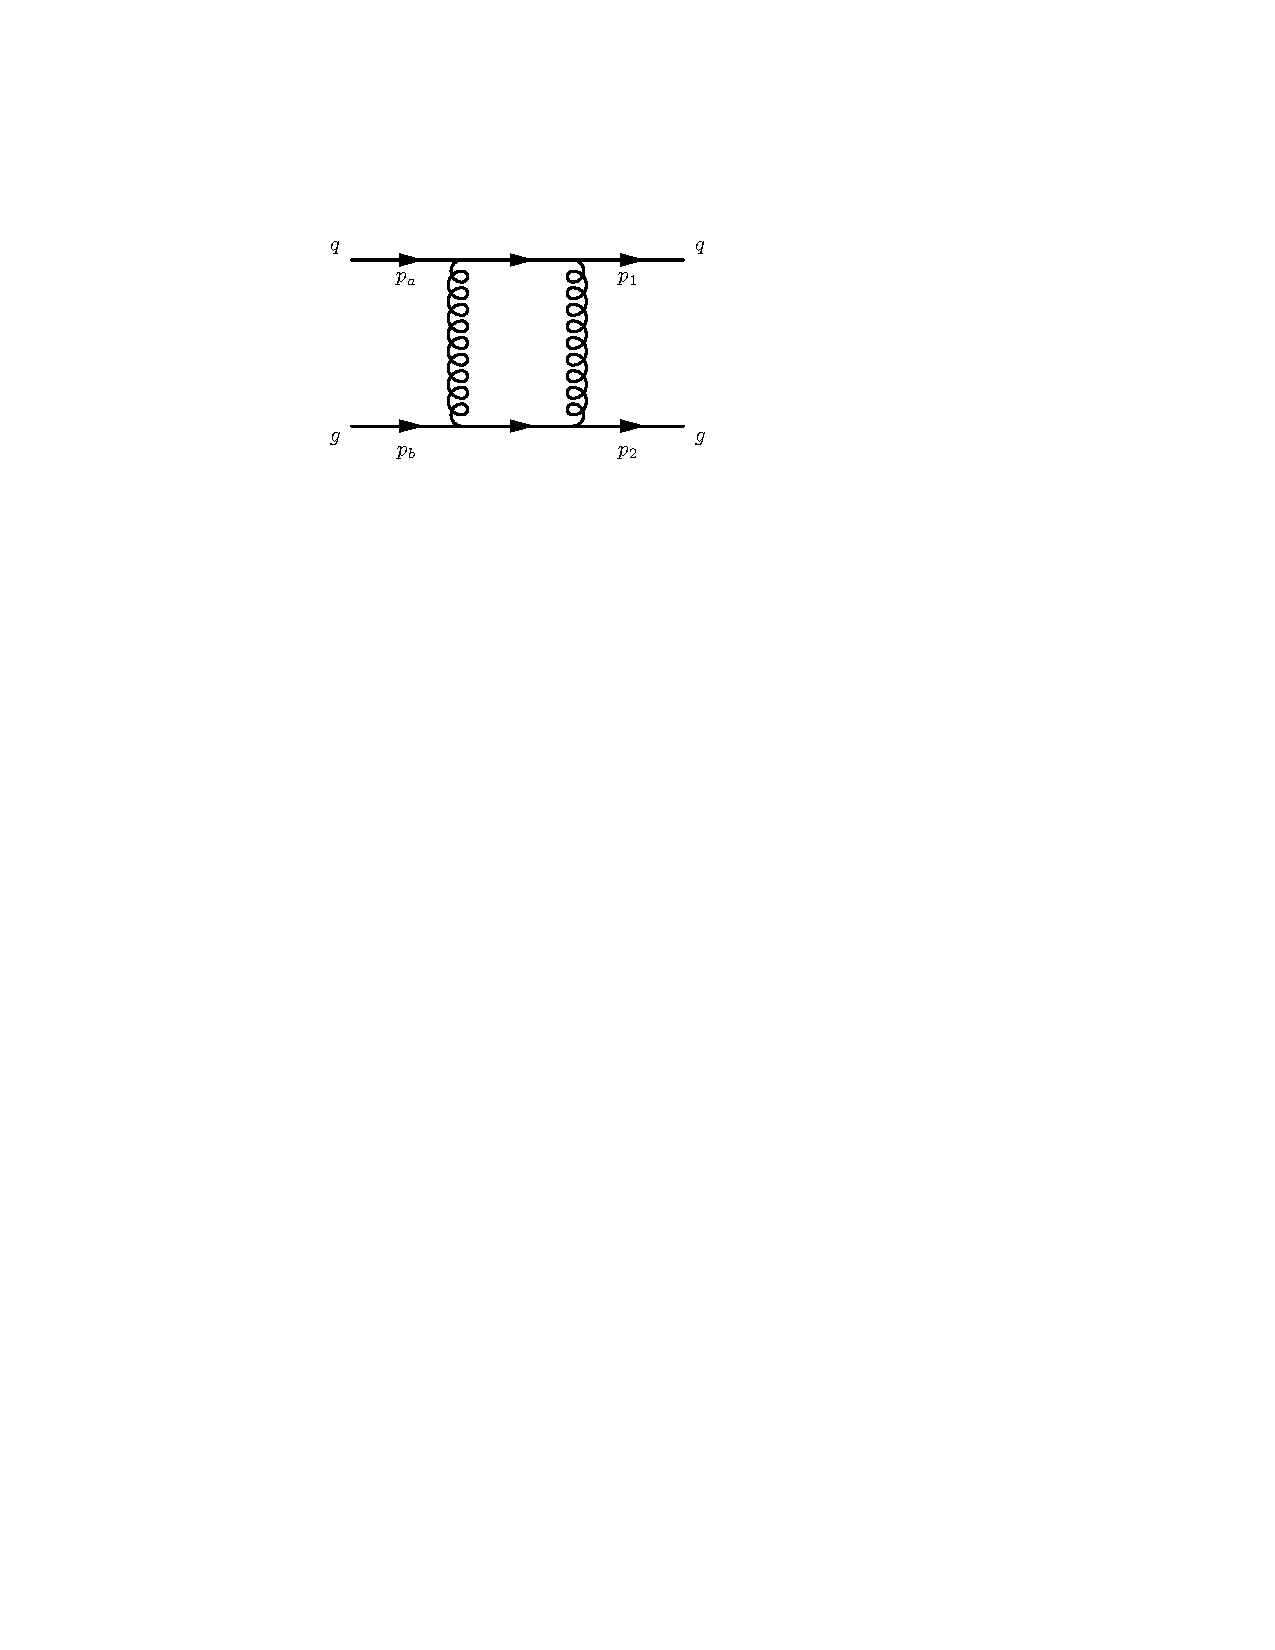
\includegraphics[width=0.8\textwidth]{NLO-uncrossed}
				\caption{}
				\label{fig:NLO-uncrossed}
			\end{subfigure}
			\begin{subfigure}[b]{0.48\textwidth}
				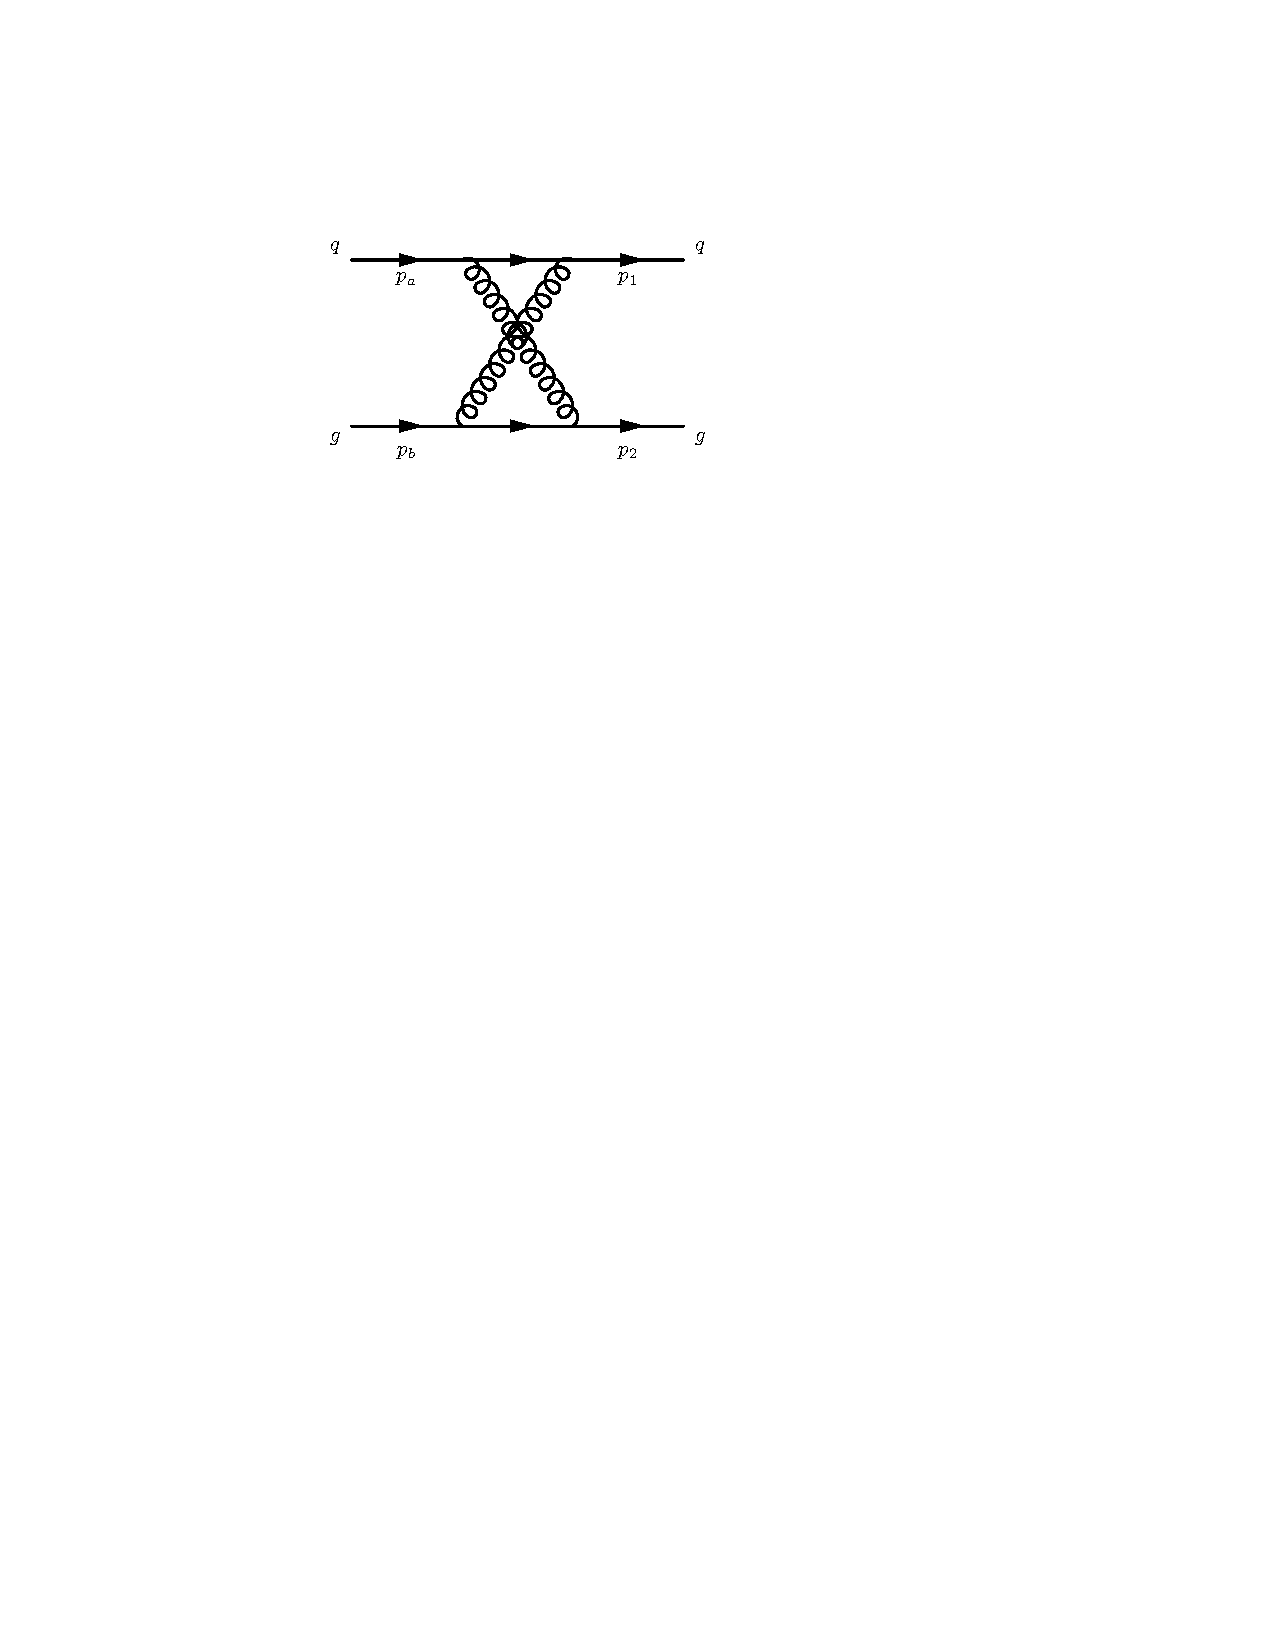
\includegraphics[width=0.8\textwidth]{NLO-crossed}
				\caption{}
				\label{fig:NLO-crossed}
			\end{subfigure}
			\caption{The leading logarithmic contributions to $qg\rightarrow qg$ at NLO.  The uncrossed
 			         exchanges two gluons in the $t$ channel and }
			\label{fig:NLO-leadingContrib.}
		\end{figure}

	\section{Effective Vertices For Real Emissions}
		\label{sub:effective_vertices_for_real_emissions}

	In order to generalise what we have done so far to higher multiplicity scattering events we begin
	by considering $qQ\rightarrow qQg$ in the high energy limit.

	\section{Virtual Corrections To All Orders}
		\label{sub:effective_vertices_for_real_emissions}

	\section{High Energy Phase-space Integration}
		\label{sub:HEPhaseSpace}

		% High energy theory
% !TEX root = thesis.tex

\chapter{$\zg$+Jets at the LHC}
\label{chap:Zs}

	Except where otherwise referenced the work in this chapter and the subsequent chapters refers to
	work undertaken by the author as part of the High Energy Jets collaboration.\\This work is the theoretical foundation for the
	full-flexible parton level Monte Carlo generator soon to be publicly available from

	\begin{center}
		\url{http://hej.web.cern.ch/HEJ/}
	\end{center}

	and is published in~\cite{ZPaper}.

\section{Introducing $\zg$+Jets at the LHC}

	The Large Hadron Collider (LHC) has opened up a new range of energies for hadronic
	collisions.  It has already been a resounding success with the discovery of the
	scalar Higgs boson completing the particle content of the Standard Model (SM).
	Hadronic colliders, by their very nature, lead to final states with large
	amounts of QCD radiation and being able to accurately describe this is
	essential.  Both the SM and many `Beyond the Standard Model' theories
	predict events with multiple hard jets in the final state and as seen in the
	previous chapter this can pose a serious problem for fixed-order descriptions.

	The current best approach for describing QCD radiation is through the use of
	a Monte Carlo (MC) generators using the principles outlined in section~\ref{sec:MC}.
	A wide range of such MC generators are available implementing everything from
	fixed-order perturbative schemes such as those described in~\cite{Mangano:2002ea,Badger:2012pg} to parton
	shower models which resum the logarithms arising from soft and collinear logarithms~\cite{Gleisberg:2008ta,Sjostrand:2007gs,Corcella:2000bw}.
	This soft and collinear radiation is experimentally observed to cascade from outgoing
	high energy quarks and gluons in chaotic patterns we refer to as jets.  While parton
	showers do a good job of describing the composition of jets they cannot be expected to give the correct
	description of the $p_T$ spectrum of events with a high multiplicity of jets.
	It is also possible to combine the
	theoretical ideas behind fixed order and parton shower predictions.  These schemes typically
	produce resummed results and then match to either leading order or next-to-leading
	results giving a formal accuracy of LO+LL~\cite{Mangano:2001xp} and NLO+LL~\cite{Alioli:2012yfa}
	respectively.  This approach gives a better description of multi-jet states however the current state-of-the-art for the
	fixed order component is still limited to next-to-leading order in $\alpha_s$ (with the
	exception of the recent $\text{N}^3$LO result~\cite{Anastasiou:2015ema}).

	In the \hej framework we aim to resum the large logarithmic corrections
	arising from well separated (in rapidity), hard final state jets.  We capture these
	important terms by calculating those
	diagrams which contribute a `leading logarithm' in the High Energy limit
	at all orders in $\alpha_s$.

	In the remainder of this chapter we discuss how we can describe the production
	of di-leptons plus multiple hard jets through the emission of an electroweak $Z^0$
	boson and an off-shell photon, $\gamma^*$.  We do this by constructing a current
	describing $\zg$ emission from one of the incoming quark or anti-quark lines and
	then combine this with a `passive' quark or gluon current as was described in
	section~\ref{sec:currents}.  The effective vertex derived in section~\ref{sec:effectiveVertices}
	can then be used to generalise the resulting matrix element to give an approximate
	description of the $(\zg\to)e^+e^- + n$ jets final state valid in the High Energy
	limit of QCD discussed in chapter~\ref{chap:HEQCD}.  The interference
	present from the multiple possible emission sites of the $\zg$ is described exactly by a
	generalisation of the $t$-channel picture which allows for multiple `chains' of
	momenta flowing through the reggeised gluons in the $t$-channel.  This approach
	requires a new regularisation procedure to carefully render the resulting
	matrix element finite when we consider the cancellation of poles from the Lipatov
	propagator terms and the effective vertices.  We also treat the interference arising
	from the two distinct emissions ($Z^0$ and $\gamma^*$) exactly.

	The formal accuracy of the description given here is LO+LL.  The leading order
	accuracy is achieved by performing a multiplicative matching to exact matrix
	elements generated using \texttt{MadGraph\_aMC@NLO}.  As discussed in section~\ref{sec:HEJ}
	this required a completely new matching set-up and this too is described later in
	this chapter along with some of the other computational challenges encountered
	along the way.

	Finally we present a comparison of results from \hej $\zg$ plus jets to several recent
	experimental studies at the LHC; both from the ATLAS collaboration and from
	the CMS experiment.  We see that we describe the data well in these studies
	and, in particular, in the regions of phase-space with large rapidity gaps and high invariant
	mass \hej gives a better description of the data than the other fixed-order and
	fixed-order plus parton shower predictions included.

\section{Constructing $\zg$+jets}
	\label{sec:Zcurrents}

	We now consider the construction of a current and an all orders
	inclusive cross-section for the $\zg$.  We start by looking at just
	the $Z^0$ emission from a single fermion line.

	\subsection{A Current for $Z^0$+Jets}
		\label{sub:zCurrent}

		For any given initial state (excluding the case of gluon-gluon scattering which will
		not contribute an FKL configuration) there are two possible emission sites for the
		$Z^0$ per fermion i.e. two for $qg$ and $\bar qg$ scattering and four for $qq$,
		$\bar qq$ and $\bar q\bar q$ scattering. The emission sites on a single fermion line
		are illustrated in fig.~\eqref{fig:emissionsites}.  In the language of currents discussed
		previously we call the left hand side of fig.~\eqref{fig:emissionsites} $j_\mu^{Z}$.
		It is given by:

		\begin{align}
		  \begin{split}
		    j^Z_\mu = \frac{C_{Zq}C_{Ze}}{p_Z^2 - M^2_Z +
		      i\Gamma_ZM_Z}\Bigg(&\frac{\bk{1}{\gu{\sigma}(\slashed p_{out} + \slashed
		        p_{e^+} + \slashed p_{e^-})\gl{\mu}}{a}}{(p_{out} + p_Z)^2} + \\
		    &\frac{\bk{1}{\gu{\mu}(\slashed p_{in} - \slashed p_{e^+} - \slashed
		        p_{e^-})\gl{\sigma}}{a}}{(p_{in} - p_Z)^2}\Bigg)\bk{e^+}{\gl{\sigma}}{e^-},
		    \label{eqn:Zcurrent}
		  \end{split}
		\end{align}

		\begin{figure}[bt]
			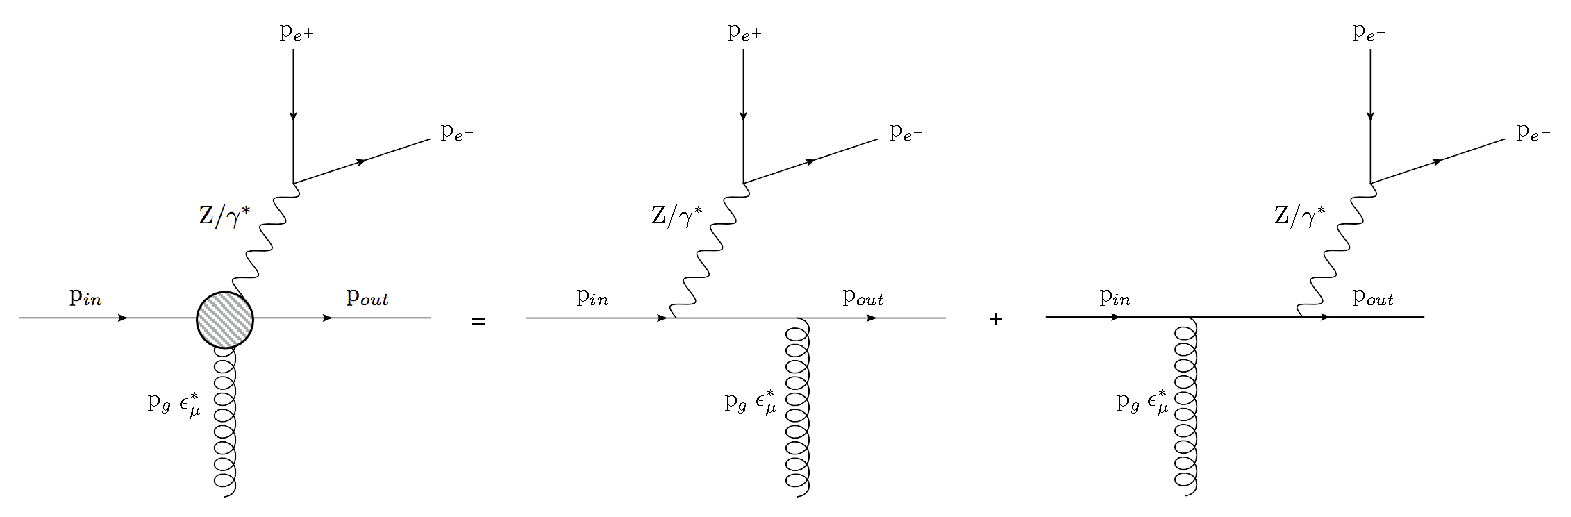
\includegraphics[width=0.98\linewidth]{figures/EmissionSites.pdf}
			\caption{The possible emission sites for a neutral weak boson.}
			\label{fig:emissionsites}
		\end{figure}

		where $M_Z$ is the mass of the $Z^0$ boson, $\Gamma_Z$ is its width, $C_{Zx}$ is
		the coupling of the $Z^0$ to $x$, $x=e,q,\nu_e,\ldots$ and $\mu$ is the Lorentz
		index for the $t$-channel gluon propagator.

		We can expand the quark and lepton momenta using their completeness relations which,
		in terms of spinor-helicity brackets, is given by:

		\begin{equation}
			\slashed p_{i} = |i_+\rangle\langle i_+| + |i_-\rangle\langle i_-|.
		\end{equation}

		This fixes the helicity of the incoming quark, $h_{\text{in}}$, and the outgoing quark,
		$h_{out}$, to be identical, and we are left with a current which only has four
		possible helicity configurations depending on $h_q = h_{\text{in}} = h_{\text{out}}$ and the
		electron helicity, $h_e$:

		\begin{align}
		  \begin{split}
		    j^Z_\mu(h_q, h_e) = &\ C_{Zq}^{h_q}C_{Ze}^{h_e}\ \frac{\bk{e^+_{h_e}}{\gl{\sigma}}{e^-_{h_e}}}{p_Z^2 -
		      M^2_Z + i\Gamma_ZM_Z} \\ &\ \times\bigg(\frac{2p_1^\sigma\bk{1_{h_q}}{\gu{\mu}}{a_{h_q}} +
		      \bk{1_{h_q}}{\gu{\sigma}}{e^+_{h_q}} \bk{e^+_{h_q}}{\gu{\mu}}{a_{h_q}} +
		      \bk{1_{h_q}}{\gu{\sigma}}{e^-_{h_q}} \bk{e^-_{h_q}}{\gu{\mu}}{a_{h_q}}}
		    {(p_{out} + p_Z)^2}\\
		    &\qquad + \frac{ 2p_a^\sigma\bk{1_{h_q}}{\gu{\mu}}{a_{h_q}} -
		      \bk{1_{h_q}}{\gu{\mu}}{e^+_{h_q}} \bk{e^+_{h_q}}{\gu{\sigma}}{a_{h_q}} -
		      \bk{1_{h_q}}{\gu{\mu}}{e^-_{h_q}} \bk{e^-_{h_q}}{\gu{\sigma}}{a_{h_q}}}
		    {(p_{in} - p_Z)^2}\bigg).
		    \label{eq:Zcurrent}
		  \end{split}
		\end{align}

		We can then express amplitudes for $Z^0$ plus jets in terms of contractions of
		a $Z^0$ emitting current with either a quark or gluon current discussed previously.  Taking
		the concrete example of $qg\to Zqg$ we can write the matrix element as follows:

		\begin{align}
		\begin{split}
			{|\bar{\mathcal{M}}_{qg\to Zqg}^{t}|}^2 =& \ \frac{g_s^2}{8}\
			\frac{1}{(p_a-p_1-p_{e^+}-p_{e^-})^2 (p_b-p_n)^2}  \sum_{h_q,h_e,h_g}|
			j^{Z}_\mu(h_q,h_e) j^{g\mu}(h_g)|^2.
		  	\label{eq:qgamp}
		\end{split}
		\end{align}

		We will investigate the behaviour of eqn.~\eqref{eq:qgamp} for a `slice' through the final state phase-space
		where each particles momenta is parametrised by:

		\begin{align*}
		\begin{split}
			p_i = &k_{i\perp}\Big(\cosh (y_i); \cos (\phi_i), \sin (\phi_i), \sinh (y_i)\Big) \\
		\end{split}
		\end{align*}

		and,

		\begin{align}
		\begin{split}
			k_{1\perp} = k_{e^+\perp} = 40\mbox{GeV}& \hspace{0.5cm} k_{e^-\perp} =
			\frac{m_Z^2}{2k_{e^+\perp}\left(\cosh(y_{e^+} - y_{e^-}) -
			    \cos(\varphi_{e^+} - \varphi_{e^-}))\right)}, \\
			\varphi_{1} =& \pi \hspace{0.5cm} \varphi_{e^+} = \pi + 0.2 \hspace{0.5cm}
			\varphi_{e^-} = -(\pi + 0.2), \\
			y_1=\Delta& \hspace{0.5cm} y_2=-\Delta \hspace{0.5cm} y_{e^+} = \Delta
			\hspace{0.5cm} y_{e^-} = \Delta - 1.5,
			\label{eq:momenta}
		\end{split}
		\end{align}

		So as $\Delta$ increases we pull the two jets apart in rapidity.  In this phase space slice
		the lepton pair are emitted in the forward region and so the physical picture is that the
		incoming quark with $p_a\sim p_1=p_+$ emits a $Z^0$ and then a $t$-channel gluon (or a
		$t$-channel gluon and \emph{then} a $Z^0$).

		We then observe the behaviour shown in fig.~\eqref{fig:ZatLO}: as we pull the
		jets apart in rapidity (i.e. as we go to large $\Delta$) we see that the matrix element
		approaches a constant; this is the result which would be obtained by using the BFKL
		formalism in which all jets are taken be infinitely well separated in rapidity.\\As we
		expect for the case of $2\to 2$ scattering we see exact agreement between our expression
		and the leading order result obtained from \texttt{MadGraph\_aMC@NLO}~\cite{Alwall:2014hca}.
		It is clear that the BFKL limit is not reached until relatively large values for $\Delta$,
		therefore it would be a poor approximation were we to just take the infinite rapidity limit
		of this as our expression for the $Z^0$ matrix element.

		\begin{figure}[hbt]
			\centering
			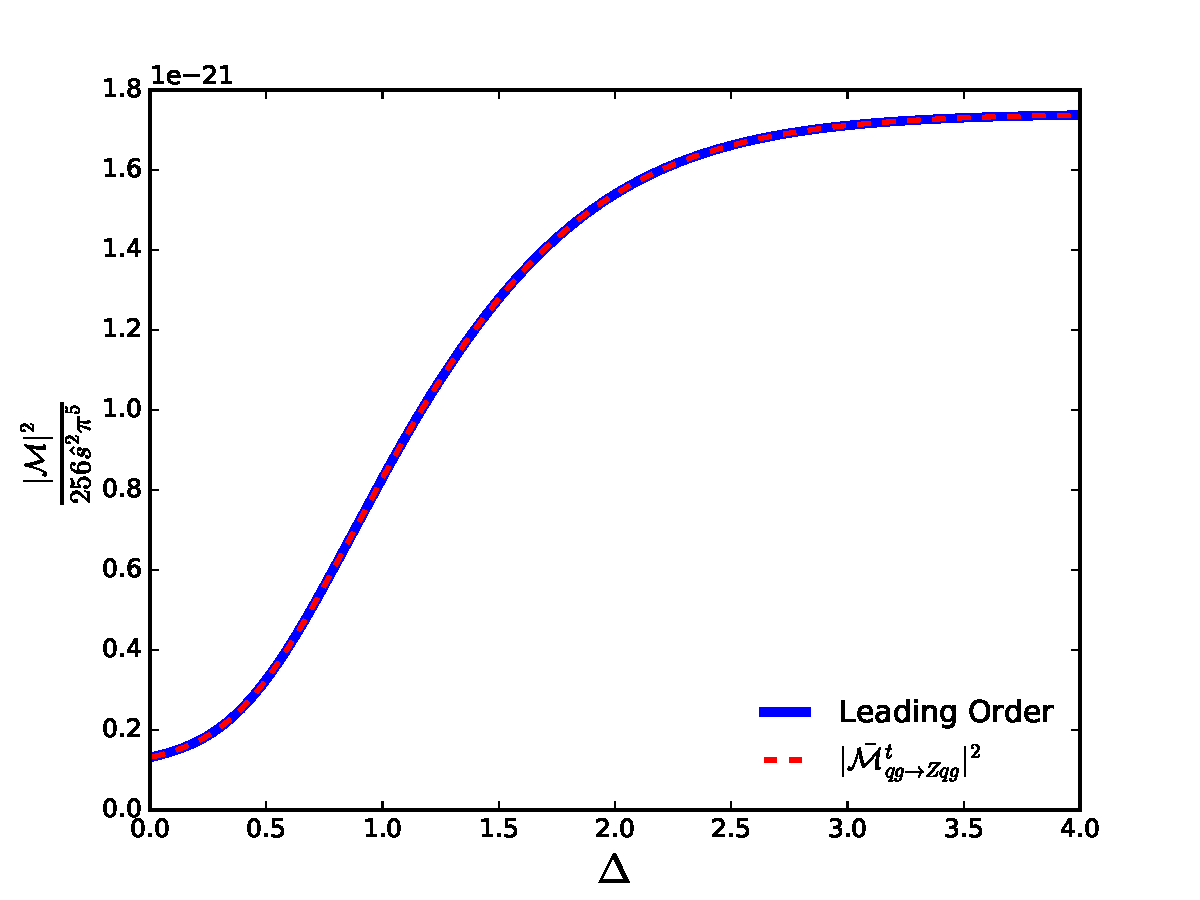
\includegraphics[width=1.0\linewidth]{Z_NoI_qg.pdf}
			\caption{$\overline{|\mathcal{M}_{qg\to Zqg}^{t}|}^2$ shown for a slice through the
			final state phase-space defined by eqn.~\eqref{eq:momenta}.  We compare to the
			leading order result obtained from \texttt{MadGraph\_aMC@NLO}.}
			\label{fig:ZatLO}
		\end{figure}

		The picture becomes more complicated when considering the $qQ\to ZqQ$ scattering since
		there are now four possible places where the (anti-)quark may emit the $Z^0$.  In
		previous work by the High Energy Jets collaboration the case of $W^\pm$ plus multiple
		hard jets was treated by attaching the boson to a single external quark line
		probabilistically~\cite{Andersen:2012gk}.  In the case of $W^\pm$ the interference
		terms arising from multiple boson emission sites is small and can be neglected, the reason for this is two
		fold. Firstly, the emission of the $W^\pm$ changes the flavour of the emitting quark line and so the
		final state will differ in almost all diagrams depending on where you emit (and hence there is no
		interference allowed), the exceptions to this are processes such as $uu\to(W^\pm\to)e+\nu_eud$ where
		either line could have been the emitter and so these are PDF suppressed. Secondly, in order to have
		interference the $W$ boson must be able to be emitted from multiple legs \emph{and} have the same charge
		wherever you attach it - again this is because the $W^\pm$ will decay to a distinct final state and no
		interference can occur. With these constraints in mind there are far fewer diagrams which contribute to the
		interference effects in $W^\pm$-plus-jets.  However as we will see later in the case of $\zg$ this leads to an approximate matrix
		element which differs significantly from the leading-order result and so here we will include not only the
		contributions to the matrix element arising from the $Z^0$ being emitted from both (anti-)quark
		legs separately but also the resulting interference term.

	\subsection{$Z^0$ Emission Interference}

		Our high-energy
		description of the matrix elements relies on the correct description of the
		$t$-channel momenta, and this obviously depends on which of the quark lines
		the $Z^0$ was emitted from.  We therefore need to modify the simple
		framework outlined above.  We will use the subscript $a$ ($b$) to label the
		current at the lowest (highest) end of the rapidity chain.  We then define $t_a$
		($t_b$) to be the $t$-channel momentum exchanged when the bosons are emitted at
		the lowest (highest) end of the rapidity chain.  Then the amplitude squared
		for $qQ\to qQ(Z^0\to) e^+ e^-$ is given by:

		\begin{align}
		\begin{split}
			{|\bar{\mathcal{M}}_{qQ\to ZqQ}^{t}|}^2 &= g_s^2 \frac{C_F}{8N_c}
			\Big|\frac{j^{Z^0}_a\cdot j_b}{t_a} + \frac{j_a\cdot
			j^{Z^0}_b}{t_b}\Big|^2\\
			&= g_s^2 \frac{C_F}{8N_c} \left( \Big|\frac{j^{Z^0}_a\cdot j_b}{t_a}\Big|^2 + \Big|\frac{j_a\cdot
			j^{Z^0}_b}{t_b}\Big|^2 + 2\Re{\Big\{\Big(\frac{j^{Z^0}_a\cdot
			j_b}{t_a}\Big)\Big(\frac{j_a\cdot j^{Z^0}_b}{t_b}\Big)^*\Big\}} \right),
			\label{eqn:interference}
		\end{split}
		\end{align}

		where $j_{a,b}$ are the pure quark currents defined previously.  The
		coupling constants of the $Z^0$ to the relevant quarks and leptons are contained
		within $j^{Z^0}(h_q,h_e)$, as in eqn.~\eqref{eqn:Zcurrent}.

		Fig.~\eqref{fig:twojets} shows the value of this matrix element squared scaled by the squared partonic
		centre-of-mass energy for increasing rapidity separation of the two jets. Once again the
		result is compared with that obtained from the full, tree-level matrix elements from
		\texttt{MadGraph\_aMC@NLO}.  The slice through phase space here is the same as that used in the
		previous section given by eqn.~\eqref{eq:momenta}.  Fig.~\eqref{fig:twojets} also
		shows the separate contributions to the total matrix element squared coming from the
		$\zg$ emission from the forward moving quark line (black, dashed) and emission
		from the backward moving quark line (green, dotted).  In this phase space slice,
		the leptons also have an increasing positive rapidity and so the forward emission
		matrix element describes the full matrix element most closely, with the contribution
		from backward-emission falling at large values of $\Delta y$.  The sum of the forward
		and backward emission matrix elements neglecting interference (magenta, dotted)
		significantly overestimates the final result.  Once the destructive interference
		effects have been taken into account, the full sum (red, solid) correctly reproduces
		the LO matrix element (blue, thick solid).  It is therefore clear that at low
		rapidities the inclusion of the interference effect plays an important r\^ole in
		the accuracy of the matrix element.

		Fig.~\eqref{fig:twojets} shows that in the region of very high rapidity separation
		the full matrix element squared (scaled by $s^2$ and an irrelevant phase space factor)
		approaches a constant.  We could have predicted this behaviour by considering
		eqn.~\eqref{eqn:HEfail2}; in the strict High Energy limit all the absolute rapidity
		information becomes lost and we only have dependence on $s$ and the transverse
		momenta of the outgoing partons (we still have information about the rapidity gap through
		$s$ using eqn.~\eqref{eqn:mandel2}).  In this case we also have the $Z^0$ propagator
		and its couplings to the partons and leptons to consider but the kinematics of the
		$t$-channel gluon still dominates.  The limit approached can be easily evaluated
		by applying the high energy limit, since in the $\Delta y\to\infty$ limit only
		the forward emission term contributes we have:

		\begin{align}
		\begin{split}
			\frac{{|\bar{\mathcal{M}}_{qQ\to ZqQ}^{HE}|}^2}{256\pi^5s^2} &= \frac{\alpha_s^2C_F^2}{64\pi^3(N_c^2-1)}
			\sum_{h_a, h_e}\frac{|C_{Za}^{h_a}C_{Ze}^{h_e}|^2}{|p_{1\perp}|^2|p_{2\perp}|^2}.
			\label{eqn:zLimit}
		\end{split}
		\end{align}

		Once we have scaled out the invariant mass squared divergence (as well as the usual phase
		space factor) out we have the limiting behaviour shown in fig~\eqref{fig:twojets}.

		\begin{figure}[hbt]
		  \begin{center}
		    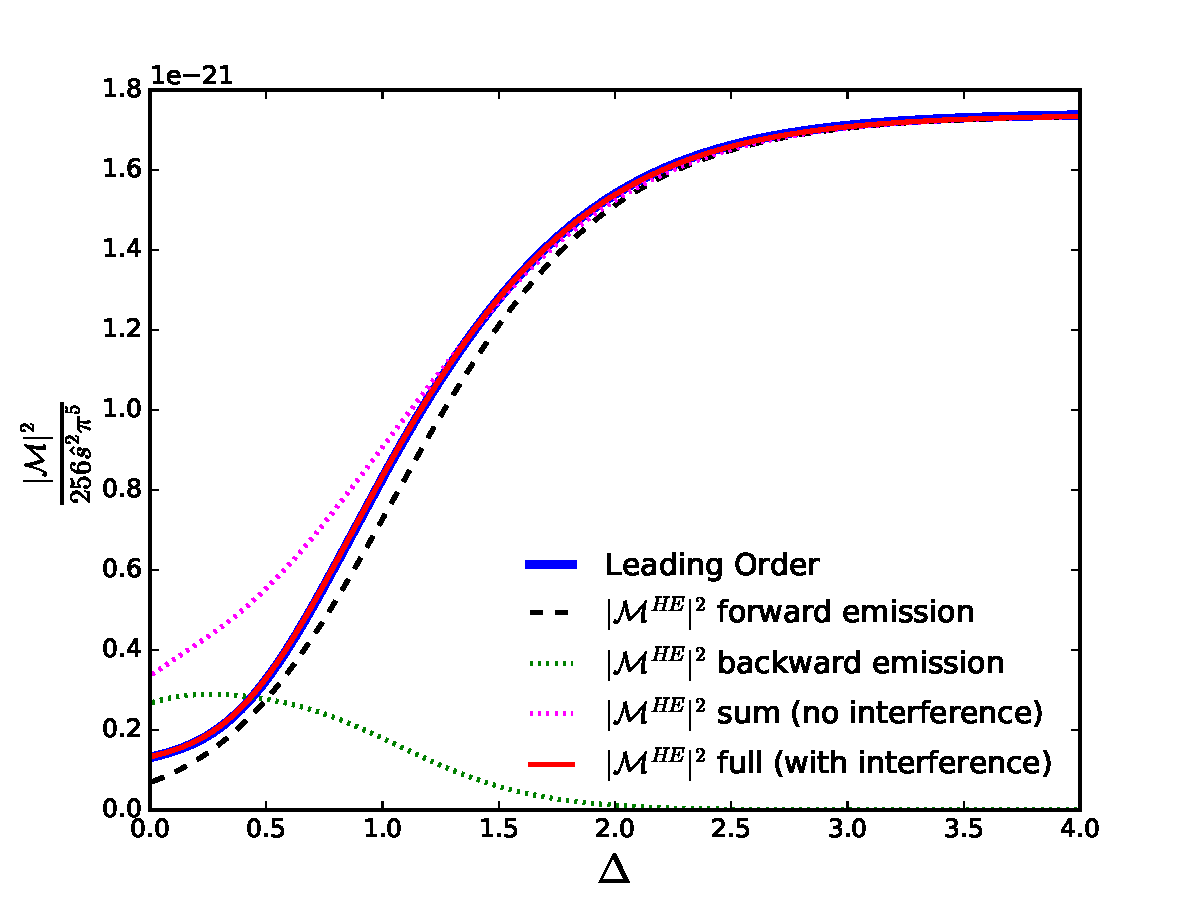
\includegraphics[width=1.0\linewidth]{slice.pdf}
		    \caption{The matrix-element squared divided by the square of the partonic
		      centre-of-mass energy for $qQ\to ZqQ$ with the $Z^0$ decaying to an
		      electron-positron pair for the phase space slice described in
		      eqn.~\eqref{eq:momenta}.  Increasing values of $\Delta$ represent
		      increasing rapidity separation between the jets.  The different lines show the contributions from
		      different terms in the calculation: only emission from the forward or the
		      backward quark line (black, dashed and green, dotted), their sum without
		      the interference term (magenta, dotted) and their sum including
		      interference (red, solid) which is seen to agree exactly with the LO result
		      (blue, thick solid).}
		    \label{fig:twojets}
		  \end{center}
		\end{figure}

	\subsection{Photonic Interference}

		Since any virtual $Z^0$ decaying to an $e^+e^-$ pair could also have proceeded via an off-shell virtual photon,
		$\gamma^*$, we must also include these processes and the resulting interference
		between the $Z^0$ and $\gamma^*$.

		The $\gamma^*$ emission matrix element is similar to that of the $Z^0$-only matrix
		element shown in eqn.~\eqref{eq:qgamp} and the same story applies with the
		possible emission sites causing interference.  All that needs to be changed is the
		propagator term and the couplings of the boson to the emitting (anti-)quark and
		the decay products.  The full current for $\zg$ emission is then obtained by summing
		the two separate currents as follows:

		\begin{align}
			\label{eq:jsum}
			j^{\zg}_\mu(h_q,h_e) = j^Z_\mu(h_q,h_e) + j^\gamma_\mu(h_q,h_e).
		\end{align}

		Then upon squaring eqn.~\eqref{eq:jsum} we will automatically include the interference
		terms from the cross-terms. The inclusion of the virtual photon terms is particularly
		important when studying a combined lepton invariant mass, $(p_{e^+} + p_{e^-})^2$,
		far from the $Z^0$ Breit-Wigner mass peak. This can be seen in fig.~\eqref{fig:DileptonMass},
		where slices through phase space are shown similarly to fig.~\eqref{fig:twojets}, but
		now for an (a) lower and (b) higher value of the di-lepton mass.  In both cases, the
		contribution of the virtual photon processes is above 25\%.

		\begin{figure}[hbtp]
		        \centering
		        \begin{subfigure}[b]{0.78\textwidth}
		                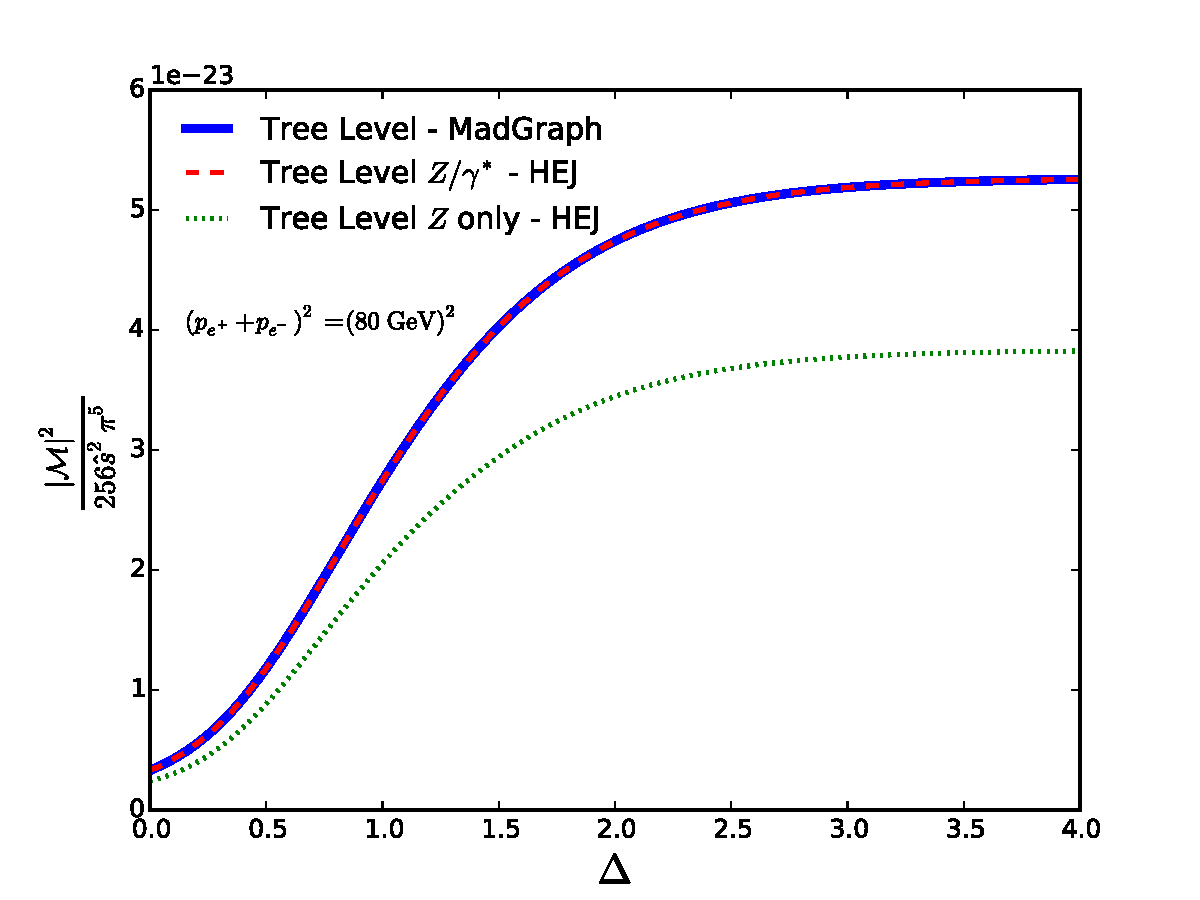
\includegraphics[width=\textwidth]{ZLowMass}
		                \caption{}
		                \label{fig:LowDileptonMass}
		        \end{subfigure}
		        ~
		        \begin{subfigure}[b]{0.78\textwidth}
		                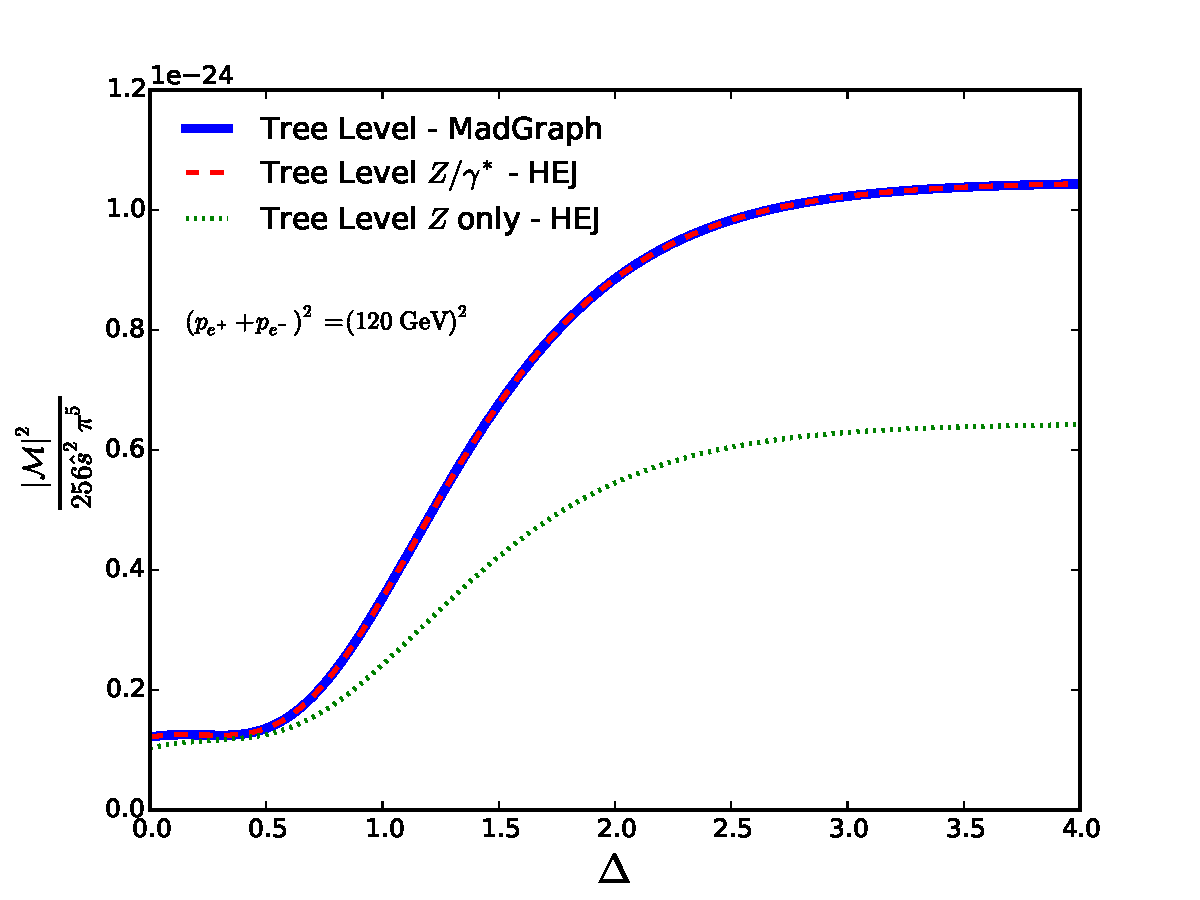
\includegraphics[width=\textwidth]{ZHighMass}
		                \caption{}
		                \label{fig:HighDileptonMass}
		        \end{subfigure}
		        \caption{The matrix-element squared divided by the square of the
		          partonic centre-of-mass energy for $qQ\to \zg qQ$ with the $\zg$ decaying
		          to an electron-positron pair.  The
		          $\mathcal{O}(\alpha_s^2 \alpha_W)$ tree-level contribution
		          as described in HEJ (red, dashed) exactly matches that of
		          \texttt{MadGraph\_aMC@NLO} (blue, solid).  The terms corresponding to the production
		          of a $Z^0$ boson only (green, dotted) significantly undershoots the
		          full result.  The
		          virtual photon terms are, therefore, clearly an important
		          contribution to the matrix element away from the $Z^0$ Breit-Wigner
		          peak.}
		        \label{fig:DileptonMass}
		\end{figure}

	\subsection{The $2\rightarrow n$ Matrix Element}

		Armed with eqn.~\eqref{eq:jsum} we can extend eqn.~\eqref{eq:qgamp} in the obvious way
		to form a complete matrix element for the emission of a $\zg$ boson.  We can also
		describe the various possibilities ($qq$, $qg$ and $gq$) simply by substituting
		the currents which apply in any given situation.  Of course, in practice we use
		the importance sampling techniques discussed in chapter~\ref{chap:HEQCD} to
		randomly sample the possible incoming parton types and so all combinations of
		currents are included.

		Following in the vein of the previous chapter we now look to extend our description
		to higher multiplicity final states.  Since our expression for the effective vertices are
		independent of the currents at either end of the $t$-chain we can write the squared matrix element for
		$qQ\to (\zg\to ) e^+e^- q (n-2)g Q$ as:

		\begin{align}
		\begin{split}
		    &|\mathcal{M}^{t}_{qQ\to \zg q(n-2)gQ}|^2 = \\&\frac{g_s^{2n}C_F}{8N_c}\
		    \ \times \Bigg( \frac{| j_a^{\zg}\cdot j_b|^2}{t_{a1}t_{a(n-1)}} \prod^{n-2}_{i=1} \frac{-\Ca V^2(q_{ai},
		      q_{a(i+1)})}{t_{ai} t_{a(i+1)}}  \\ & + \ \frac{|j_a \cdot j_b^{\zg} |^2}{t_{b1}t_{b(n-1)}}
		    \prod^{n-2}_{i=1}\frac{-\Ca V^2(q_{bi}, q_{b(i+1)})}{t_{bi} t_{b(i+1)}}  \\
		    &-\ \frac{2\Re\{(j_a^{\zg}\cdot j_b)({j_a \cdot
		        j_b^{\zg}})^*\}}{\sqrt{t_{a1}t_{b1}}\sqrt{t_{a(n-1)} t_{b(n-1)}}}
		    \prod^{n-2}_{i=1}\frac{\Ca V(q_{ai}, q_{a(i+1)})\cdot V(q_{bi},
		      q_{b(i+1)})}{\sqrt{t_{ai}t_{bi}} \sqrt{t_{a(i+1)}t_{b(i+1)}}}\Bigg).
			\label{eq:allorderreal}
		\end{split}
		\end{align}

		In the case of $n=2$, this reduces back to eqn.~\eqref{eqn:interference}.  If
		either $a$ or $b$ is an incoming gluon then there are only two possible emission sites
		for the $\zg$ once again and therefore we only need calculate one $t$-channel momenta chain
		and one can set the relevant $j_a^{\zg}$ or $j_b^{\zg}$ to
		zero in eqn.~\eqref{eqn:interference}.

		Fig.s~\eqref{fig:3jslice} and~\eqref{fig:4jslice} show the phase space
		slices for $qQ\to(\zg\to)e^+e^-qgQ$ and $qQ\to(\zg\to)e^+e^-qggQ$
		respectively, we see the same behaviour as observed for the 2 jet final state described in
		fig.~\eqref{fig:ZatLO}.  For these higher multiplicity final states we only
		approximate the leading order matrix element however we see that at large rapidity separations
		our approximation converges to the exact result as indeed it must in the High Energy limit.

		Eqn.~\eqref{eq:allorderreal} gives us the all-orders real corrections to $\zg$ plus jets which we wish to sum for all $n$.
		However, before proceeding to calculate the cross-section we must carefully render eqn.~\eqref{eq:allorderreal}
		finite by including the corresponding virtual corrections whose divergences will cancel the pathologies
		in the effective vertices.

		\begin{figure}[hbt]
		  \begin{center}
		    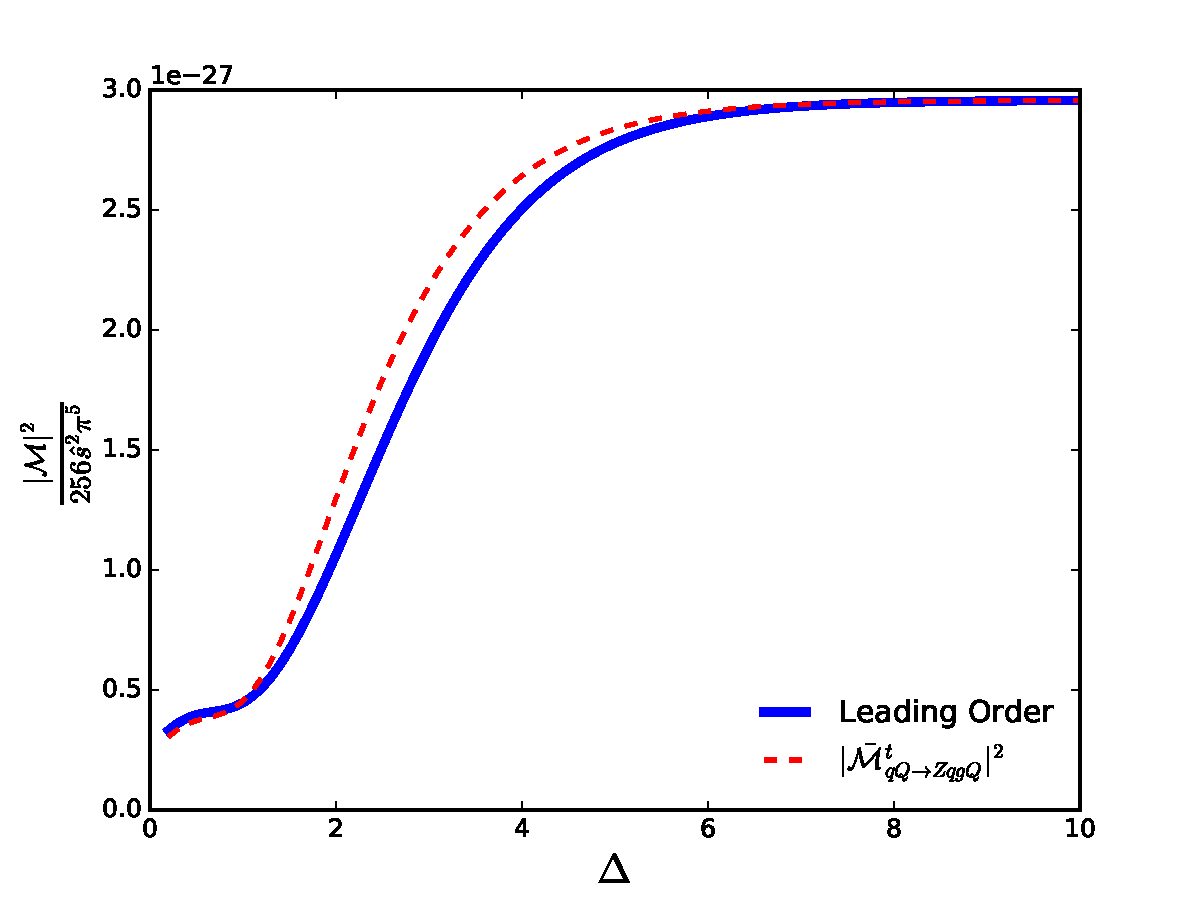
\includegraphics[width=1.0\linewidth]{slice3j.pdf}
		    \caption{A slice through phase space for the $\zg$+ 3 jet final state.  The slice defined is
		    akin to that described for the 2 jet case in fig.~\eqref{fig:ZatLO} where as $\Delta$ increases
		    we pull apart all three jets and the leptonic decay products are emitted increasingly far into
		    the forward direction.}
		    \label{fig:3jslice}
		  \end{center}
		\end{figure}

		\begin{figure}[hbt]
		  \begin{center}
		    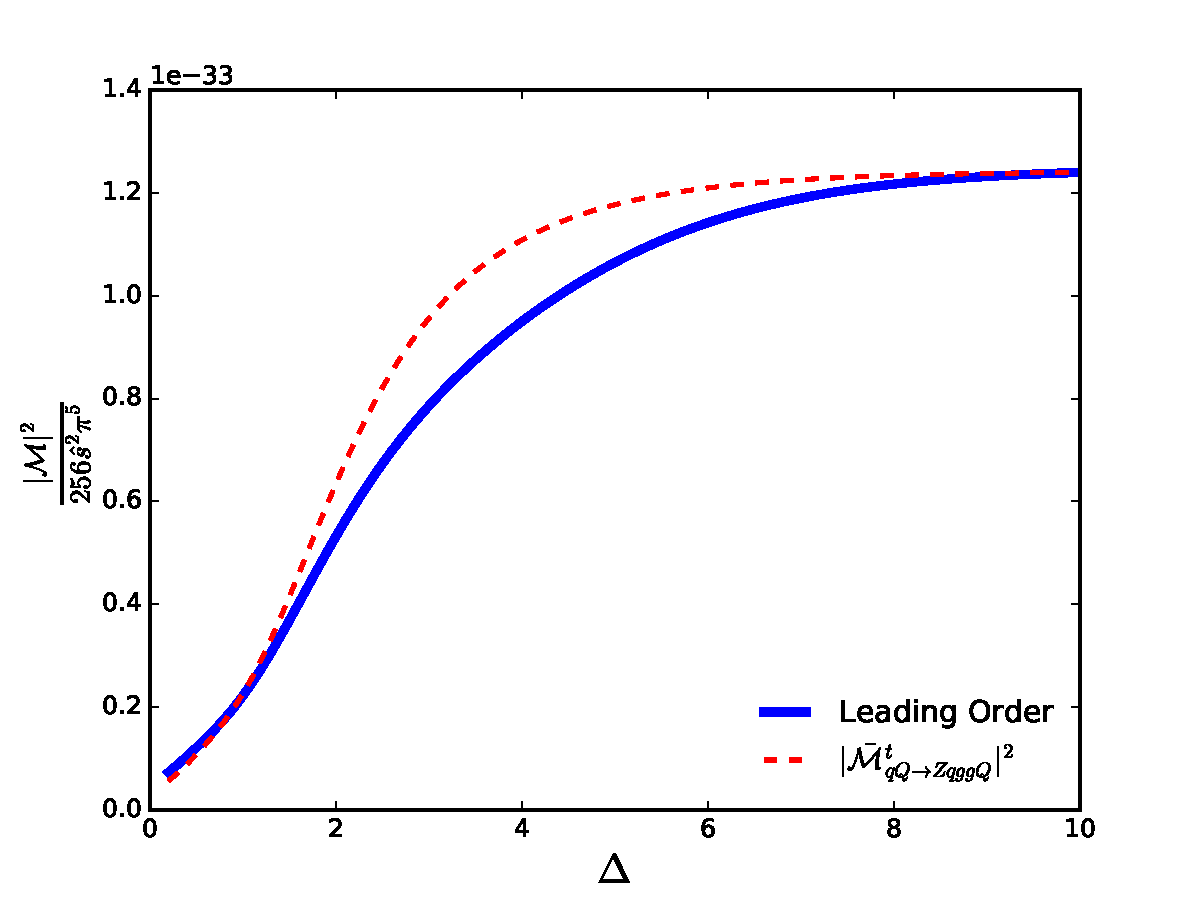
\includegraphics[width=1.0\linewidth]{slice4j.pdf}
		    \caption{A slice through phase space for the $\zg$+ 3 jet final state.  The slice defined is
		    akin to that described for the 2 and 3 jet case shown in fig.~\eqref{fig:ZatLO} and
		    fig.~\eqref{fig:3jslice} respectively.}
		    \label{fig:4jslice}
		  \end{center}
		\end{figure}

\section{Regularising the $\zg$+Jets Matrix Element}
	\label{sec:regularising}

	\subsection{Real Soft Emissions}
		\label{sub:softEmissions}

		To calculate useful quantities such as cross sections etc. we must integrate equation
		eqn.~\eqref{eq:allorderreal} over all of phase space.  However, as discussed in chapter~\ref{chap:theory}
		problems arise when we attempt to integrate over the soft regions of phase space.  It is well understood
		that the divergences coming from soft real emissions cancel with those coming from
		virtual emissions and so we must explicitly show this cancellation and calculate the remaining
		finite contribution multiplying the $(n-1)$-final state parton matrix element.

		In the previous work on $W^\pm$ emission the finite remainder from this cancellation was found
		to be~\cite{Andersen:2009nu, Andersen:2008gc}:

		\begin{equation}
			\frac{\alpha_s C_a \Delta_{j-1, j+1}}{\pi}\ln{\frac{\lambda_{cut}^2}{|\vec{q}_{j\perp}|^2}},
		\end{equation}

		where $\Delta_{i-1, i+1}$ is the rapidity span of the final state partons either side of our
		soft emission and $|\vec{q}_{j\perp}|^2$ is the sum of squares of the transverse components of
		the $j^{th}$ $t$-channel gluon momenta.  $\lambda_{cut}$ is a parameter we choose which \emph{defines}
		the soft region.  That is, any real emission satisfying $p^2 \geq \lambda_{cut}^2$ we consider a hard perturbative
		emission while any emission with $p^2 < \lambda_{cut}^2$ we consider too soft to be resolved.\\
		Here we investigate
		the cancellation of these divergences for $Z^0$ emission and most importantly whether the finite term
		is of the same form for the interference term which was previously excluded.\\We start by looking
		at a $2\rightarrow n$ process and take the limit of one final state parton momentum, $p_i$, becoming
		small.  Because of the form of eqn.~\eqref{eq:allorderreal} this amounts to looking at the
		effect of an external gluon becoming soft on our expression for the effective vertex for real emissions.

		We can immediately see that for $p_i$ going soft the gluon `chain' momenta going into,
		and coming out of, the $j^{th}$ emission site will coincide: $q_{j+1}\sim q_j$, therefore:

		\begin{equation}
			V^\rho(q_j, q_{j+1}) = -2q_j^\rho - 2\left(\frac{s_{aj}}{s_{ab}} -
				\frac{q^2_{j}}{s_{bj}}\right)p_b^\rho + 2\left(\frac{s_{bj}}{s_{ab}} +
				\frac{q_j^2}{s_{aj}}\right)p_a^\rho
				\label{eqn:vertexlimit}
		\end{equation}

		Furthermore we can see that the two final terms from the bracketed expressions will dominate
		as $p_j\to0$ and so we can approximate the full vertex by:

		\begin{equation}
			V^\rho(q_j, q_{j+1}) \sim -2\frac{q^2_{j}}{s_{bj}}p_b^\rho + 2\frac{q_j^2}{s_{aj}}p_a^\rho.
				\label{eqn:vertexlimit2}
		\end{equation}

		In eqn.~\eqref{eq:allorderreal} we have three terms involving the effective vertex;
		quadratic terms like $V^2(q_{tj}, q_{t(j+1)})$ and $V^2(q_{bj}, q_{b(j+1)})$ and interference terms
		like $V(q_{tj}, q_{t(j+1)})\cdot V(q_{bj}, q_{b(j+1)})$.  The procedure for the $V^2$ terms follows
		similarly for both the quadratic top-line emission and bottom-line emission terms and so only
		the calculation for top-line emission is shown here.

		\subsubsection{$V^2(q_{tj}, q_{t(j+1)})$ Terms}

			Upon squaring eqn.~\eqref{eqn:vertexlimit2} and imposing the on-shell conditions for
			$p_a$ and $p_b$ we have:

			\begin{equation}
				V^2(q_{ti}, q_{ti}) = - \frac{4s_{ab}}{s_{bi}s_{ai}}q^4_{ti}
				\label{eqn:temp}
			\end{equation}

			We must now explicitly calculate the invariant mass terms.  Since we are in the
			High Energy regime we have that $p_a^+\gg p_a^-, p_{a\perp}$ and $p_b^+\gg p_b^-, p_{b\perp}$
			therefore we may take:

			\begin{align}
				s_{ab}= 2p_a\cdot p_b \sim 2p^+_ap^-_b,\\
				s_{bi}= 2p_b\cdot p_i \sim 2p^-_bp^+_i,\\
				s_{ai}= 2p_a\cdot p_i \sim 2p^+_ap^-_i.
			\end{align}

			Using this we can write eqn.~\eqref{eqn:temp} as:

			\begin{equation}
				V^2(q_{ti}, q_{ti}) = - \frac{4}{|\vec{p}_{1\perp}|^2}q^4_{ti},
				\label{eqn:temp2}
			\end{equation}

			Now looking back to eqn.~\eqref{eq:allorderreal} we see that each vertex is associated with factors of
			$q^{-2}_{ti}q^{-2}_{t(i+1)}$ but since the emission is soft $q_{ti}=q_{t(i+1)}$ and this becomes $q^{-4}_{ti}$.
			That factor conspires to cancel with the corresponding factor of $q^{4}_{ti}$ in eqn.~\eqref{eqn:temp2}.
			Including the additional factors of $C_A$ and $g_s$ the finite factor remaining is given by:

			\begin{equation}
				\frac{4C_Ag_s^2}{|\vec{p}_\perp|^2},
				\label{eqn:finalsoft}
			\end{equation}

		\subsubsection{$V(q_{ti}, q_{t(i+1)})\cdot V(q_{bi}, q_{b(i+1)})$ Terms}

			Taking the mixed dot-product of the two vertex terms we have:

			\begin{equation}
				V(q_{ti}, q_{ti})\cdot V(q_{bi}, q_{bi}) = -\frac{s_{ab}}{s_{ai}s_{bi}}t_{ti}t_{bi}
			\end{equation}

			having simplified the expression using $p_a^2=0$ and $p_b^2=0$ once again.  The invariant mass terms
			here are identical to those we saw in the $V^2$ terms and the products of $t_{ti}t_{bi}$ also appear
			in the denominator of the interference term in eqn.~\eqref{eq:allorderreal}.
			After this cancellation we are left with exactly what we had before in eqn.~\eqref{eqn:finalsoft}.
			Since exactly the same factor comes from all three terms at the amplitude squared level we may factor
			them out and express the amplitude squared for an $n$-parton final state with one soft emission in
			terms of an $(n-1)$-parton final state amplitude squared multiplied by a common factor:

			\begin{equation}
				\lim_{p_i\rightarrow0} |\mathcal{A}_{Z/\gamma}^{2\rightarrow n}|^2 = \left(\frac{4C_Ag_s^2}{|\vec{p}_{i\perp}|^2}\right)
					|\mathcal{A}_{Z/\gamma}^{2\rightarrow (n-1)}|^2
				\label{eqn:apparent}
			\end{equation}

		\subsubsection{Integration of Soft Divergences}

			As discussed above the divergences contained in eqn.~\eqref{eqn:apparent} only become
			apparent after we have attempted to integrate over phase space.  The Lorentz
			invariant phase space integral associated with $p_i$ is given by:

			\begin{equation}
				\int\frac{d^3\vec{p_i}}{(2\pi)^32E_i}\frac{4C_Ag_s^2}{|\vec{p}_\perp|^2}.
			\end{equation}

			It is convenient to replace the integral over the $z$-component of momentum with one over rapidity,
			$y_2$.  Rapidity and transverse momentum are related through the definition of rapidity given
			in eqn.~\eqref{eqn:rap}.  The Jacobian of this transformation is given by:

			\begin{align*}
				\frac{dy}{dp_z} &= \frac{1}{2(E+p_z)} \frac{\partial}{\partial p_z}(E+p_z) - \frac{1}{2(E-p_z)}\frac{\partial}{\partial p_z}(E-p_z),\\
				&= \frac{E}{E^2-p_z^2} - \frac{p_z}{E^2-p_z^2}\frac{\partial E}{\partial p_z},\\
				&= \frac{E}{E^2-p_z^2} - \frac{p_z}{E^2-p_z^2}\frac{p_z}{E},\\
				&= \frac{1}{E},
			\end{align*}

			and therefore the rewritten phase space integral then reads:

			\begin{equation}
				\int_{\text{soft}}\frac{d^{2+2\epsilon}\vec{p}_{\perp}}{(2\pi)^{2+2\epsilon}}\int_{y_{i-1}}^{y_{i+1}}\frac{dy}{4\pi}\frac{4C_Ag_s^2}
					{|\vec{p}_\perp|^2}\mu^{-2\epsilon} = \frac{4C_Ag_s^2\mu^{-2\epsilon}}{(2\pi)^{2+2\epsilon}4\pi}
					\Delta_{i-1, i+1}\int_0^{\lambda_{\text{cut}}}\frac{d^{2+2\epsilon}\vec{p}_{\perp}}{|\vec{p}_\perp|^2},
			\end{equation}

			where we have analytically continued the integral to $2+2\epsilon$ dimensions to regulate the anticipated
			divergences and introduced the parameter $\mu$ to keep the coupling dimensionless in the process.
			We have also introduced an upper bound on the transverse momentum integration of $\lambda_{\text{cut}}$ -
			this parameter will be discussed in more detail later.  Converting to polar coordinates and using
			the result for the volume of a unit hypersphere gives the integrated soft contribution:

			\begin{equation}
				\frac{4C_Ag_s^2}{(2\pi)^{2+2\epsilon}4\pi}\Delta_{i-1, i+1}
				\frac{1}{\epsilon}\frac{\pi^{1+\epsilon}}
				{\Gamma(\epsilon+1)}\left(\frac{\lambda_{cut}^2}{\mu^2}\right)^\epsilon.
				\label{eqn:soft}
			\end{equation}

			As promised eqn.~\eqref{eqn:soft} is clearly divergent in the limit where $\epsilon\to0$.

	\subsection{Virtual Emissions}

		As discussed in chapter~\ref{chap:HEQCD} the virtual emission diagrams are included
		using the Lipatov ansatz for the gluon propagator:

		\begin{equation}
			\frac{1}{q_i^2}\longrightarrow\frac{1}{q_i^2}e^{\hat{\alpha}(q_i)\Delta_{i,i-1}},
		\end{equation}

		where:

		\begin{equation}
			\hat{\alpha}(q_i) = \alpha_sC_Aq_i^2\int \frac{d^{2+2\epsilon}k_{\perp}}{(2\pi)^{2+2\epsilon}}
			\frac{1}{k^2_\perp(k_\perp - q_{i\perp})^2}\mu^{-2\epsilon}.
			\label{eqn:feynmanPs}
		\end{equation}

		To see the cancellation of the infrared $\epsilon$ poles we must perform the integral
		explicitly using dimensional regularisation. Using Feynman parameters to re-express
		eqn.~\eqref{eqn:feynmanPs}:

		\begin{align}
			\hat{\alpha}(q_i) &= \alpha_sC_Aq_i^2\int \frac{d^{2+2\epsilon}\hat{k}_{\perp}}{(2\pi)^{2+2\epsilon}}\int_0^1
				\frac{dx}{[\hat{k}^2 _\perp + q_{i\perp}^2(1-x)]^2}\mu^{-2\epsilon},
		\end{align}

		where we have performed a change of variables to $\hat{k}_\perp = k_\perp - xq_{i\perp}$
		Changing the order of integration we can perform the $\hat{k}_\perp$ integral
		using the following result:

		\begin{equation}
			\int \frac{d^dk}{(2\pi)^d}\frac{1}{(k^2 - C)^\alpha} = \frac{1}{(4\pi)^{\frac{d}{2}}}
				\frac{\Gamma(\alpha - \frac{d}{2})}{\Gamma(\alpha)}
				\frac{(-1)^\alpha}{C^{\alpha - \frac{d}{2}}},
		\end{equation}

		to give:

		\begin{align}
			\hat{\alpha}(q_i) &= -\frac{2g_s^2C_A}{(4\pi)^{2+\epsilon}}\frac{\Gamma(1-\epsilon)}{\epsilon}
			\left(\frac{q_{i\perp}^2}{\mu^2}\right)^\epsilon,
		\end{align}

		having completed the $x$ integral and used the definition $\alpha_s=\frac{g_s^2}{4\pi}$.

	\subsection{Cancellation of Infrared Divergences}
		\label{sub:cancellation}

		We now have all the necessary ingredients to show how the infrared contributions from
		soft real emissions and virtual emissions cancel leaving our integrated matrix element
		finite.  The only subtlety being that we must sum two diagrams with different multiplicity
		final states to see the cancellation.  This is because they are experimentally indistinguishable;
		the $2\rightarrow (n-1)$ virtual diagram has $(n-1)$ resolvable partons in the final state
		and we only `see' $(n-1)$ of the final states partons from $2\rightarrow n$ process because
		we consider one of the emissions too soft to resolve.\\
		The matrix element squared for the real emission diagram with one soft parton
		will look like:

		\begin{align}
		\begin{split}
			|\mathcal{A}_{Z/\gamma}^{2\rightarrow n}|^2 = \left(\frac{4g_s^2C_a}{|p_{i\perp}|^2}\right)
				\Bigg[&\left|\mathcal{K}_a j_1^{Z/\gamma}\cdot j_2\right|^2
				\frac{\prod^{n-2}_{i\neq j}V^2(q_{ti},
				q_{t(i+1)})}{\prod^{n-1}_{i\neq j}q^2_{ti}} + \\
				&\left|\mathcal{K}_b j_2^{Z/\gamma}\cdot j_1\right|^2
				\frac{\prod^{n-2}_{i\neq j}V^2(q_{bi}, q_{b(i+1)})}{\prod^{n-1}_{i\neq j}q^2_{bi}} + \\
				&2\Re\{\mathcal{K}_a\overline{\mathcal{K}_b} \times
				(j_1^{Z/\gamma}\cdot j_2)(\overline{j_2^{Z/\gamma}\cdot j_1})\}\\
				&\times\frac{\prod^{n-2}_{i\neq j}V(q_{ti}, q_{t(i+1)})\cdot V(q_{bi}, q_{b(i+1)}))}
				{\prod^{n-1}_{i\neq j}q_{ti}q_{bi}}\Bigg],
		\end{split}
		\end{align}

		where we have taken the $i^{th}$ gluon to be soft.  After including the virtual corrections
		via the insertion of the Lipatov ansatz the $2\rightarrow (n-1)$ matrix element squared is:

		\begin{align}
		\begin{split}
			|\mathcal{A}_{Z/\gamma}^{2\rightarrow (n-1)}|^2 = &\left|\mathcal{K}_a j_1^{Z/\gamma}\cdot j_2\right|^2
				\frac{\prod^{n-3}_{i}V^2(q_{ti}, q_{t(i+1)})}{\prod^{n-2}_{i}q^2_{ti}}e^{2\hat{\alpha}(q_{ti})\Delta_{i-1,i+1}} + \\
				&\left|\mathcal{K}_b j_2^{Z/\gamma}\cdot j_1\right|^2 \frac{\prod^{n-3}_{i}V^2(q_{bi}, q_{b(i+1)})}
				{\prod^{n-2}_{i}q^2_{bi}}e^{2\hat{\alpha}(q_{bi})\Delta_{i-1,i+1}} + \\
				&2\Re\{\mathcal{K}_a\overline{\mathcal{K}_b} \times (j_1^{Z/\gamma}\cdot j_2)(\overline{j_2^{Z/\gamma}\cdot j_1})\}\\
				&\times\frac{\prod^{n-3}_{i}V(q_{ti}, q_{t(i+1)})\cdot V(q_{bi}, q_{b(i+1)}))}{\prod^{n-2}_{i}q_{ti}q_{bi}}
				e^{(\hat{\alpha}(q_{bi}) + \hat{\alpha}(q_{bi}))\Delta_{i-1,i+1}},
		\end{split}
		\end{align}

		We can now go through term-by-term to show the divergences cancel and find the finite contribution to
		the matrix element squared.  Similarly to when we calculated the soft terms the arguments for the pure
		top- and bottom-line emissions follow similarly and so here we will only state the procedure for
		the top emission.\\For the top line emission we identify the following terms that will appear in the
		sum of the $2\rightarrow (n-1)$ virtual and $2\rightarrow n$ real matrix elements.  The finite
		contribution, $\mathcal{F}_{\text{top}}$, to the matrix element is given by:

		\begin{equation}
			\mathcal{F}_{\text{top}} = \frac{4C_Ag_s^2}{(2\pi)^{2+2\epsilon}4\pi}\Delta_{i-1, i+1}
			\frac{1}{\epsilon}\frac{\pi^{1+\epsilon}}
			{\Gamma(\epsilon+1)}\left(\frac{\lambda_{cut}^2}{\mu^2}\right)^\epsilon +
			e^{2\hat{\alpha}(q_{ti})\Delta_{i-1,i+1}}.
		\end{equation}

		Extracting the relevant power of the strong coupling from the
		exponential and substituting for $\hat{\alpha}(q_i)$ gives:

		\begin{align}
		\begin{split}
			\mathcal{F}_{\text{top}} &= \frac{4C_Ag_s^2}{(2\pi)^{2+2\epsilon}4\pi}\Delta_{i-1, i+1}\frac{1}{\epsilon}\frac{\pi^{1+\epsilon}}
			{\Gamma(\epsilon+1)}\left(\frac{\lambda_{cut}^2}{\mu^2}\right)^\epsilon - -\frac{2g_s^2C_A}{(4\pi)^{2+\epsilon}}
			\frac{\Gamma(1-\epsilon)}{\epsilon}\left(\frac{q_{ti\perp}^2}{\mu^2}\right)^\epsilon, \\
			&= \frac{g_s^2C_A}{4^{1+\epsilon}\pi^{2+\epsilon}}\Delta_{i-1, i+1}\left(\frac{1}{\epsilon\Gamma(1+\epsilon)}
			\left(\frac{\lambda_{cut}^2}{\mu^2}\right)^\epsilon - \frac{\Gamma(1-\epsilon)}{\epsilon}
			\left(\frac{q_{ti\perp}^2}{\mu^2}\right)^\epsilon\right).
		\end{split}
		\end{align}

		Expanding the terms involving the regularisation parameter for small values,
		$\epsilon\to0$, yields:

		\begin{equation}
			\mathcal{F}_{\text{top}} = \frac{\alpha_sC_A\Delta_{i-1, i+1}}{\pi}
			\ln\left(\frac{\lambda_{cut}^2}{q_{ti\perp}^2}\right) + \mathcal{O}(\epsilon),
		\end{equation}

		where we have used:

		\begin{align}
		\begin{split}
			\frac{1}{\Gamma(1+\epsilon)} &= 1 + \gamma_E\epsilon + \mathcal{O}(\epsilon^2),
			\Gamma(1-\epsilon) = 1 + \gamma_E\epsilon + \mathcal{O}(\epsilon^2),\\
			\left(\frac{x}{y}\right)^\epsilon &= 1 + \epsilon\ln\left(\frac{x}{y}\right) +
			\mathcal{O}(\epsilon^2).
		\end{split}
		\end{align}

		Similarly, for the terms arising from the bottom quark-line emission we have:

		\begin{equation}
		\mathcal{F}_{\text{bottom}} = \frac{\alpha_sC_A\Delta_{i-1, i+1}}{\pi}\ln\left(\frac{\lambda_{cut}^2}{q_{bi\perp}^2}\right),
		\end{equation}

		Lastly, for the interference terms we expand the exponential with both top-line emission, $q_{ti}$,
		momenta and bottom-line emission, $q_{bi}$, momenta to get:

		\begin{align}
		\begin{split}
			\mathcal{F}_{\text{interf.}} &= \frac{g_s^2C_A\Delta_{i-1, i+1}}{4^{1+\epsilon}\pi^{2+\epsilon}}
			\Big(\Big(\frac{1}{\epsilon} + \gamma_E +  \ln\Big(\frac{\lambda_{cut}^2}{\mu^2}\Big) +
			\mathcal{O}(\epsilon)\Big) - \\
			&\hspace{0.75cm}\frac{1}{2}\Big[\frac{2}{\epsilon} + 2 \gamma_E +
			\ln\Big(\frac{q_{ti\perp}^2}{\mu^2}\Big)
			- \ln\Big(\frac{q_{bi\perp}^2}{\mu^2}\Big) +
			\mathcal{O}(\epsilon)\Big]\Big) \\
			&= \frac{\alpha_sC_A\Delta_{i-1, i+1}}{\pi}\ln\Bigg(\frac{\lambda_{cut}^2}{\sqrt{q_{ti\perp}^2
			q_{bi\perp}^2}}\Bigg).
			\label{eqn:result}
		\end{split}
		\end{align}

		Eqn.~\eqref{eqn:result} is a new result which allows the inclusion of the interference terms shown
		to be important in previous discussion.  We can now express the regulated $qQ\to \zg q(n-2)gQ$
		matrix element as follows:

		\begin{align}
		  \label{eq:allordereg}
		  \begin{split}
		    &|\mathcal{M}^{HEJ-{\rm reg}}_{qQ\to \zg q(n-2)gQ}|^2 =\ g_s^2 \frac{C_F}{8N_c}\ ( g_s^2
		    \Ca)^{n-2}\  \\  \times \Bigg(& \frac{| j_a^{\zg}\cdot
		      j_b|^2}{t_{a1}t_{a(n-1)}}
		    \exp(\omega^0(q_{a(n-1)\perp})\Delta y_{n-1}) \prod^{n-2}_{i=1} \frac{-V^2(q_{ai},
		      q_{a(i+1)})}{t_{ai} t_{a(i+1)}} \exp(\omega^0(q_{ai\perp})\Delta y_i)\\
		    +\ &\frac{|j_a \cdot j_b^{\zg} |^2}{t_{b1}t_{b(n-1)}} \exp(\omega^0(q_{b(n-1)\perp})\Delta y_{n-1})
		    \prod^{n-2}_{i=1}\frac{-V^2(q_{bi}, q_{b(i+1)})}{t_{bi} t_{b(i+1)}} \exp(\omega^0(q_{bi\perp})\Delta y_i) \\
		    -\ &\frac{2\Re\{ (j_a^{\zg}\cdot j_b)(\overline{j_a \cdot
		        j_b^{\zg}})\}}{\sqrt{t_{a1}t_{b1}}\sqrt{t_{a(n-1)} t_{b(n-1)}}} \exp(\omega^0(\sqrt{q_{a(n-1)\perp}q_{b(n-1)\perp}})\Delta y_{n-1})\\
		    & \; \prod^{n-2}_{i=1}\frac{V(q_{ai}, q_{a(i+1)})\cdot V(q_{bi},
		      q_{b(i+1)})}{\sqrt{t_{ai}t_{bi}} \sqrt{t_{a(i+1)}t_{b(i+1)}}}\exp(\omega^0(\sqrt{q_{ai\perp}q_{bi\perp}})\Delta y_{i})\Bigg),
		  \end{split}
		\end{align}

		where we have defined

		\begin{align}
		  \label{eq:omega0}
		  \omega^0(q_{\perp}^2) = - \frac{g_s^2 \Ca}{4\pi^2} \ln\left( \frac{q_\perp^2}{\lambda_{cut}^2}\right).
		\end{align}

		There is one final improvement we can make to eqn.~\eqref{eq:allordereg}.  The expressions
		we obtain upon taking the soft limit of the three effective vertex terms, $V^2_t$, $V^2_b$
		and $V_t\cdot V_b$, are not exact and there are sub-leading terms which we can account for.
		We therefore have to account for the difference between, e.g $-V^2(q_{i-1},q_{i})/(t_{i-1} t_i)$,
		and its strict limit of $4/p_{i\perp}^2$ for values of $p_{i\perp}$ below $\lambda_{cut}$.  In
		practice, we include this correction for $c_{cut}<|p_\perp|<\lambda_{cut}$ with
		$c_{cut} = 0.2$~GeV and find stable results around this value (see section~\ref{sec:indep-lambd}).

		We are, at last, in a position to move forward and form an expression for an all-orders
		gauge invariant \emph{finite} matrix element for $\zg$ plus jets.  Before pressing on
		we now discuss an example calculation showing explicitly the finite nature of
		matrix element expression.

	\subsection{An Explicit Check: $2\rightarrow3$ Scattering}

		\begin{figure}[bth]
			\centering
			\begin{subfigure}[b]{0.48\textwidth}
				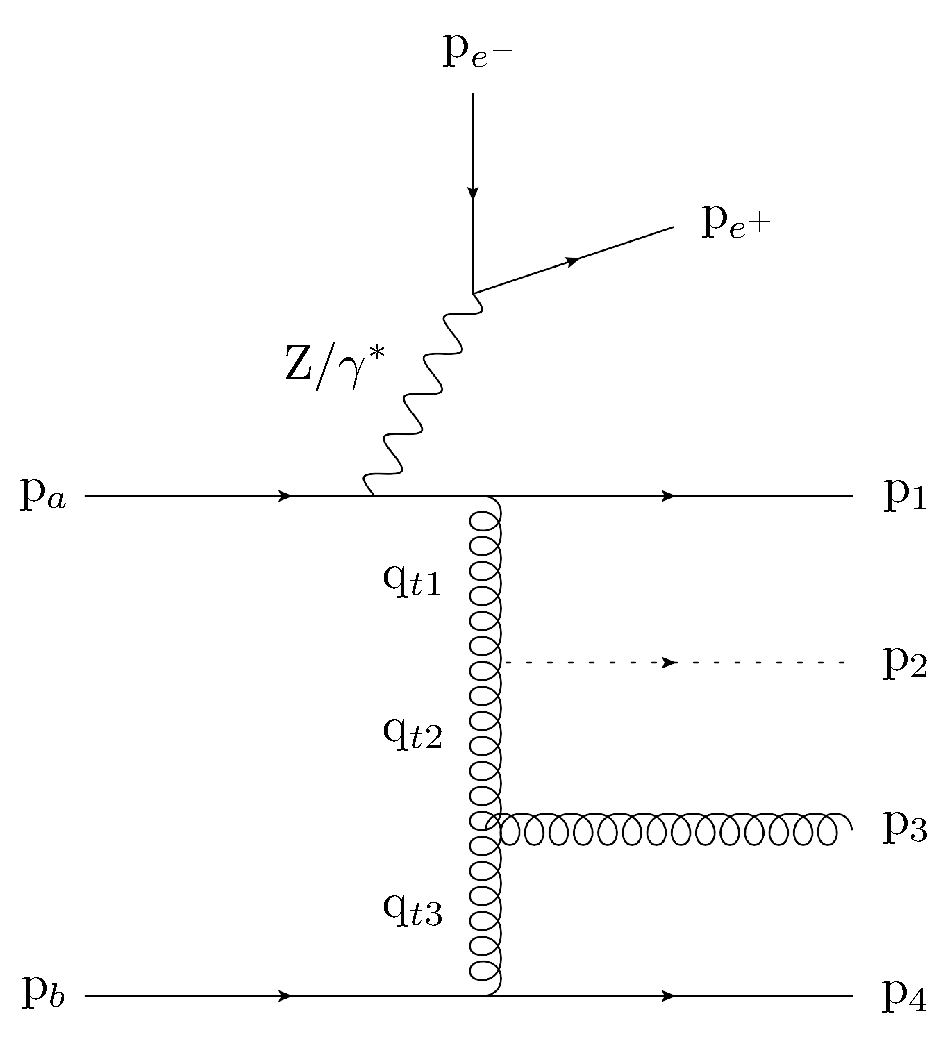
\includegraphics[width=1.0\linewidth]{RealSoftEmissionZ.pdf}
				\caption{}
				\label{fig:real24}
			\end{subfigure}
			\begin{subfigure}[b]{0.48\textwidth}
				\centering
				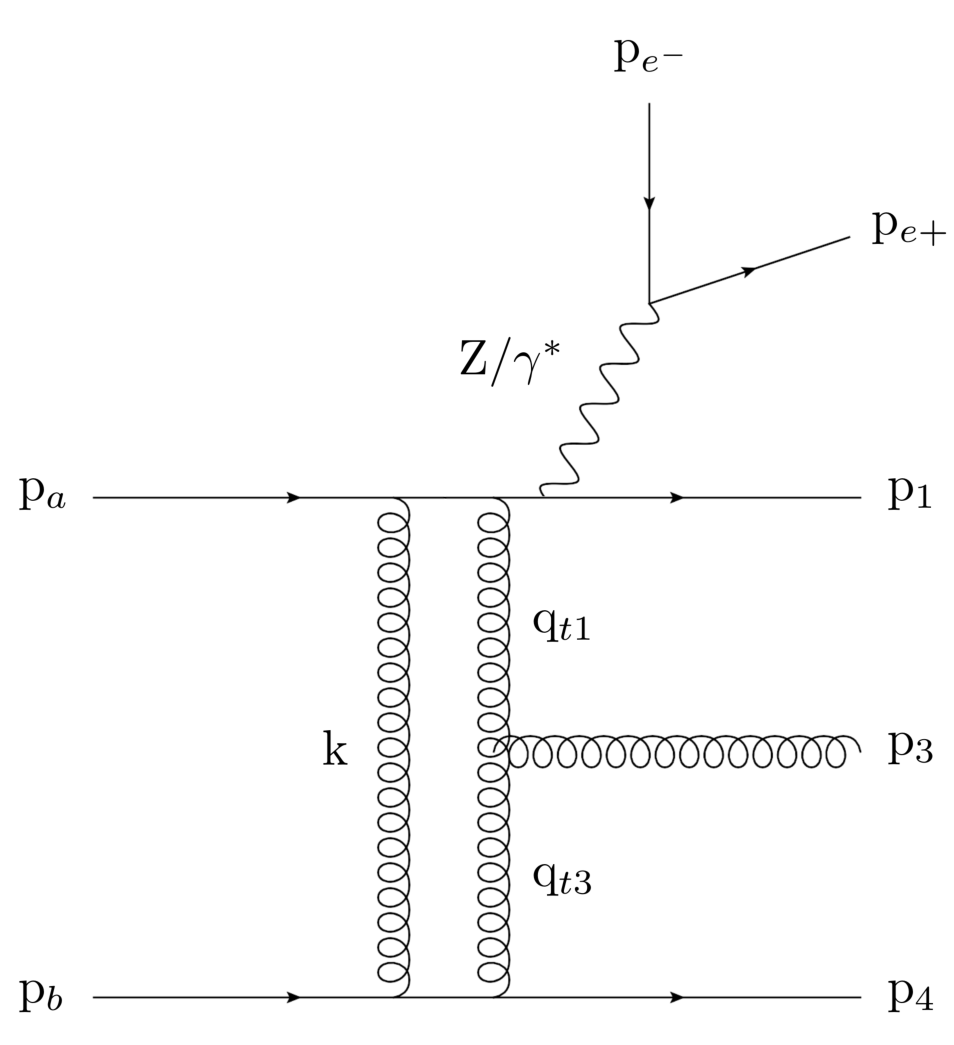
\includegraphics[width=1.0\linewidth]{VirtualSoftEmissionZ.pdf}
				\caption{}
				\label{fig:virtual23}
			\end{subfigure}

			\caption{Examples of both real and virtual diagrams contributing to
			$2\rightarrow3$ scattering. In fig.~\eqref{fig:real24} the $p_2$ has been
			drawn with a dashed line to denote it is not resolvable.  In
			fig.~\eqref{fig:virtual23} the final state momenta have been labelled in a
			seemingly strange way - this was done to make clear the cancellation
			when working through the algebra.}
			\label{fig:2to}
		\end{figure}

		Consider the case of $2\rightarrow3$ scattering where on of the final state momenta, $p_2$, has become soft.  A contributing
		soft diagram is shown in fig.~\eqref{fig:real24} and one example of a contributing virtual
		diagram of the same order is shown in fig.~\eqref{fig:virtual23}. When $p_2$ goes soft we have
		the following form for the $2\rightarrow3$ integrated amplitude squared ({N.B.}: The
		integration is only schematic and doesn't represent the full Lorentz invariant phase space):

		\begin{align}
		\begin{split}
			\int dPS|\mathcal{A}^{2\rightarrow3}_{soft}|^2 = &\frac{4C_Ag_s^2\Delta_{1,3}}{(2\pi)^{2+2\epsilon}4\pi}
			\frac{\pi^{\epsilon+1}}{\epsilon\Gamma(\epsilon+1)}
			\left(\frac{\lambda_{cut}^2}{\mu^2}\right)^\epsilon\Bigg[|\mathcal{K}_aj_1^Z\cdot j_2|^2
			\frac{V^2(q_{t1}, q_{t3})}{q^2_{t1}q^2_{t3}} \\
			+ |\mathcal{K}_bj_1\cdot j_2^Z|^2
			\frac{V^2(q_{b1}, q_{b3})}{q^2_{b1}q^2_{b3}} +
			& 2\Re\left\{\mathcal{K}_a\overline{\mathcal{K}_b}
			(j_1^Z\cdot j_2)\overline{(j_1\cdot j_2^Z)}\right\} \frac{V(q_{t1}, q_{t3})
			\cdot V(q_{b1}, q_{b3})}{q_{t1}q_{t3}q_{b1}q_{b3}}\Bigg],
		\end{split}
		\end{align}

		and the virtual contributions for the $2\rightarrow3$ amplitude are:

		\begin{align}
		\begin{split}
			\int dPS&|\mathcal{A}^{2\rightarrow3}_{virtual}|^2 = |\mathcal{K}_bj_1\cdot j_2^Z|^2
			\frac{V^2(q_{t1}, q_{t3})}{q_{t1}^2}e^{2\hat{\alpha}(q_{t1})\Delta_{1,3}} + \\
			&|\mathcal{K}_tj_1^Z\cdot j_2|^2 \frac{V^2(q_{b1}, q_{b3})}{q_{b1}^2}e^{2\hat{\alpha}(q_{b1})\Delta_{1,3}} +  \\
			& 2\Re\left\{\mathcal{K}_a\overline{\mathcal{K}_b}  (j_1^Z\cdot j_2)\overline{(j_1\cdot j_2^Z)}\right\}
			\frac{V(q_{t1}, q_{t3})\cdot V(q_{b1}, q_{b3})}{q_{t1}q_{t3}q_{b1}q_{b3}}e^{(\hat{\alpha}(q_{t1}) +
			\hat{\alpha}(q_{b1}))\Delta_{1,3}}.
		\end{split}
		\end{align}

		Once we expand the exponential to the correct order in $g_s^2$, the sum of these
		matrix elements squared over the region of phase space when $p_2$ is soft is:

		\begin{align}
		\begin{split}
			\int dPS&\left(|\mathcal{A}^{2\rightarrow3}_{soft}|^2 + |\mathcal{A}^{2\rightarrow3}_{virtual}|^2\right) =\\
			&|\mathcal{K}_aj_1^Z\cdot j_2|^2 \frac{V^2(q_{t1}, q_{t3})}{q_{t1}^2}
			{\Bigg(\frac{4C_Ag_s^2\Delta_{1,3}}{(2\pi)^{2+2\epsilon}4\pi}\frac{\pi^{\epsilon+1}}
			{\epsilon\Gamma(\epsilon+1)} - 2\hat{\alpha}(q_{t1})\Delta_{1,3}\Bigg)} + \\
			& |\mathcal{K}_bj_1\cdot j_2^Z|^2 \frac{V^2(q_{b1}, q_{b3})}{q_{b1}^2}
			{\Bigg(\frac{4C_Ag_s^2\Delta_{1,3}}{(2\pi)^{2+2\epsilon}4\pi}\frac{\pi^{\epsilon+1}}
			{\epsilon\Gamma(\epsilon+1)} - 2\hat{\alpha}(q_{b1})\Delta_{1,3}\Bigg)}+ \\
			&2\Re\left\{\mathcal{K}_a\overline{\mathcal{K}_b}  (j_1^Z\cdot j_2)\overline{(j_1\cdot j_2^Z)}\right\}
			\frac{V(q_{t1}, q_{t3})\cdot V(q_{b1}, q_{b3})}{q_{t1}q_{t3}q_{b1}q_{b3}}\\
			&{\Bigg(\frac{4C_Ag_s^2\Delta_{1,3}}{(2\pi)^{2+2\epsilon}4\pi}\frac{\pi^{\epsilon+1}}{\epsilon\Gamma(\epsilon+1)} -
			(\hat{\alpha}(q_{t1}) + \hat{\alpha}(q_{b1}))\Delta_{1,3}\Bigg)} + \mathcal{O}(g_s^4),
			\label{eqn:sjhdfa}
		\end{split}
		\end{align}

		The bracketed terms in eqn.~\eqref{eqn:sjhdfa} are exactly the cancellations calculated in section 4 above and therefore:

		\begin{align}
		\begin{split}
			\int dPS\left(|\mathcal{A}^{2\rightarrow3}_{soft}|^2 + |\mathcal{A}^{2\rightarrow3}_{virtual}|^2\right) =&
			\frac{\alpha_sC_A\Delta_{1,3}}{\pi}\Bigg(|\mathcal{K}_aj_1^Z\cdot j_2|^2 \frac{V^2(q_{t1},
			q_{t3})}{q_{t1}^2}\ln\left(\frac{\lambda_{cut}^2}{|q_{1t\perp}|^2}\right)+ \\
			& |\mathcal{K}_bj_1\cdot j_2^Z|^2 \frac{V^2(q_{b1}, q_{b3})}{q_{b1}^2}\ln
			\left(\frac{\lambda_{cut}^2}{|q_{1b\perp}|^2}\right)+ \\
			&2\Re\left\{\mathcal{K}_a\overline{\mathcal{K}_b}  (j_1^Z\cdot j_2)\overline{(j_1\cdot j_2^Z)}\right\}
			\frac{V(q_{t1}, q_{t3})\cdot V(q_{b1}, q_{b3})}{q_{t1}q_{t3}q_{b1}q_{b3}}\\
			&\ln\left(\frac{\lambda_{cut}^2}{\sqrt{|q_{1t\perp}|^2|q_{1b\perp}|^2}}\right)\Bigg) + \mathcal{O}(\alpha_s^2),
		\end{split}
		\end{align}

		which is manifestly finite.

\section{Subtractions and the $\lambda_{cut}$ scale}
	\label{sec:indep-lambd}

	We now show the stability of the High Energy Jets predictions with respect to the
	$\lambda_{cut}$ scale described above.\\We
	increase our sensitivity to the parameter by showing results for FKL momentum
	configurations only.  The non-FKL samples which are added to give the total
	cross sections have no dependence on $\lambda_{cut}$ and would therefore dilute
	any dependence in the full sample.  We begin with tab.~\eqref{tab:lambdaxs} where we show the value of
	the cross section for different values of $\lambda_{cut}$ for exclusive 2-, 3-
	and 4-jet samples.  The cuts applied are the same as in section~\ref{sub:ATLASZsec}.
	It is clear that the cross section does not display a large dependence on the
	value of $\lambda_{cut}$.

	\begin{table}[hbt!]
		\begin{center}
		\begin{tabular}{| c | c | c | c |}
		\hline
		$\lambda_{cut}$ (GeV) & $\sigma(2j)$ ($pb$) & $\sigma(3j)$ ($pb$) & $\sigma(4j)$ ($pb$) \\ \hline
		0.2 & $5.03 \pm 0.02$ & $0.70 \pm 0.02$ & $0.13 \pm 0.03$ \\
		0.5 & $5.05 \pm 0.01$ & $0.70 \pm 0.01$ & $0.13 \pm 0.01$ \\
		1.0 & $5.09 \pm 0.01$ & $0.71 \pm 0.01$ & $0.13 \pm 0.01$ \\
		2.0 & $5.16 \pm 0.04$ & $0.72 \pm 0.01$ & $0.13 \pm 0.01$ \\ \hline
		\end{tabular}
		\caption{The FKL-only cross sections for the 2-, 3- and 4-jet exclusive rates
		with associated statistical errors shown for different values of the regularisation parameter
		$\lambda_{cut}$.  The scale choice was half the sum over all transverse scales in the event, $H_T/2$.}
		\label{tab:lambdaxs}
		\end{center}
	\end{table}

	Fig.~\eqref{fig:lambdadist} shows the effect of the same variation in $\lambda_{cut}$ on the
	differential distribution in both the rapidity gap between the two leading jets in $p_\perp$,
	$\Delta y_{j1, j2}$, (a)--(c), and the rapidity gap between the two extremal jets in
	rapidity, $\Delta y_{jf, jb}$, (d)--(f).  Results are shown for exclusive 2-, 3-
	and 4-jet samples in each case.The distributions also show a very weak
	dependence on the choice of $\lambda_{cut}$.
	In practice, our default chosen value for $\lambda_{cut}$ is 0.2.

	\begin{figure}[H]
		\centering
		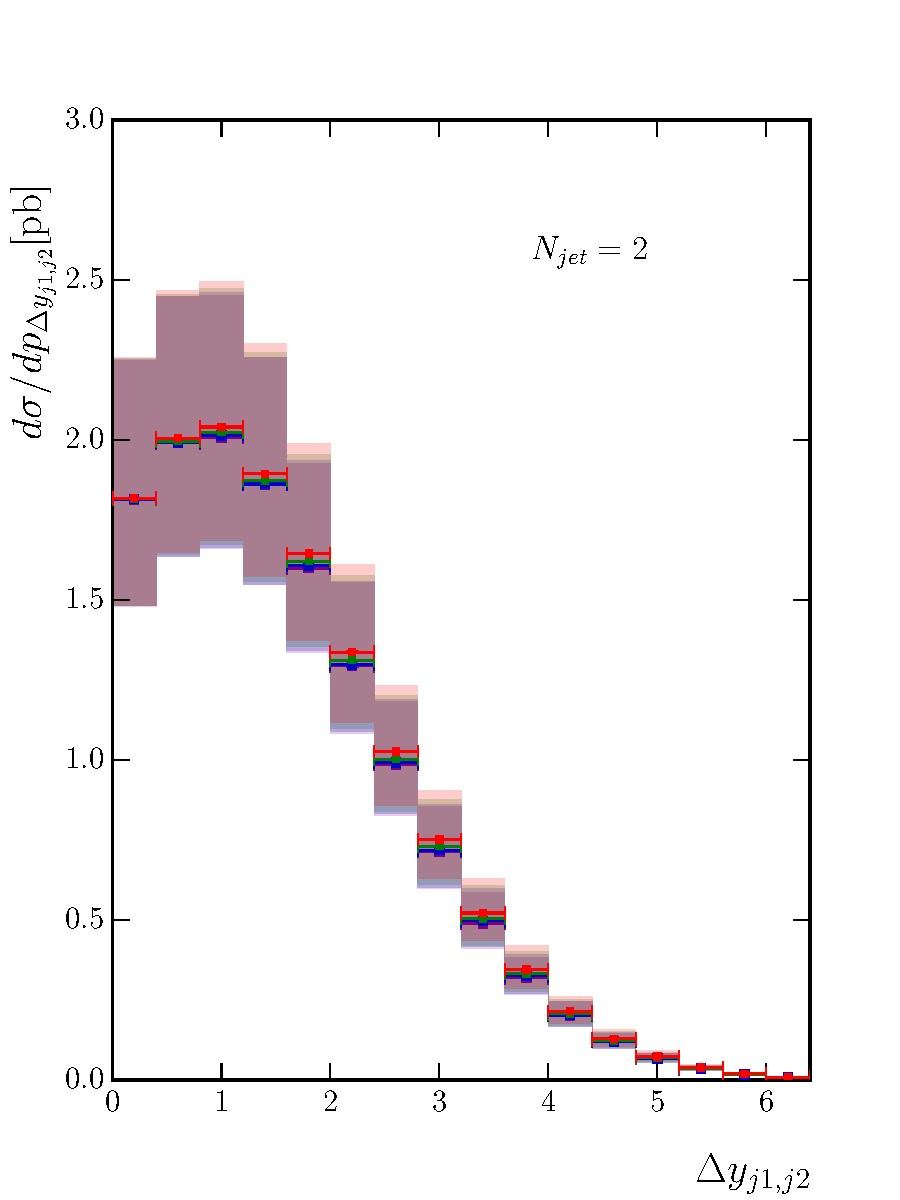
\includegraphics[width=.32\textwidth]{Z_11a_2j.pdf}\hfill
		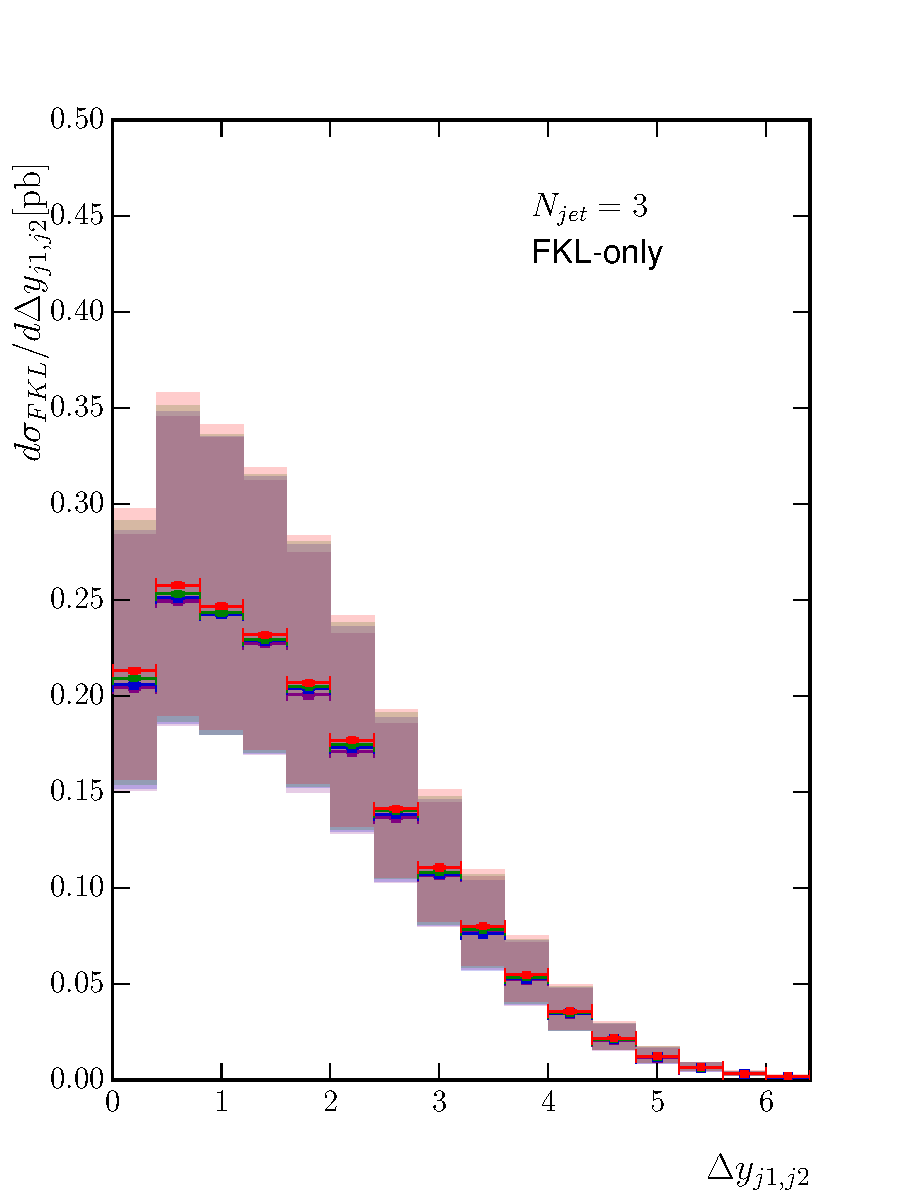
\includegraphics[width=.32\textwidth]{Z_11a_3j.pdf}\hfill
		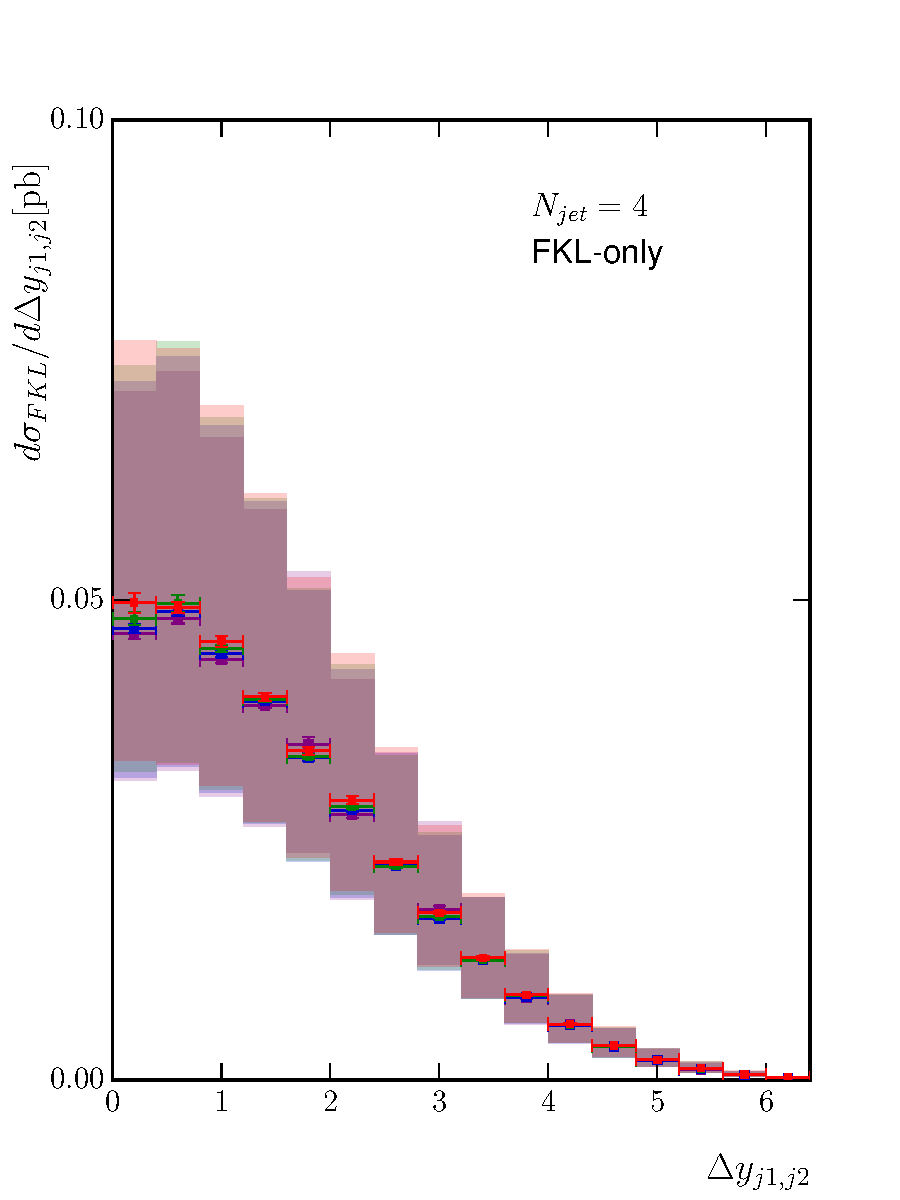
\includegraphics[width=.32\textwidth]{Z_11a_4j.pdf}
		\caption{The effect of varying $\lambda_{cut}$ on the differential distribution
		in the rapidity gap between the two leading jets in $p_\perp$, $\Delta y_{j1, j2}$,
		with the $N_{jet}=2,3,4$ exclusive selections shown from left to right.
		$\lambda_{cut}=0.2$ (red), 0.5 (blue), 1.0 (green), 2.0 (purple).
		The bands represent the scale variation described in the text.}
		\label{fig:lambdadist}
	\end{figure}

	\begin{figure}[H]
		\centering
		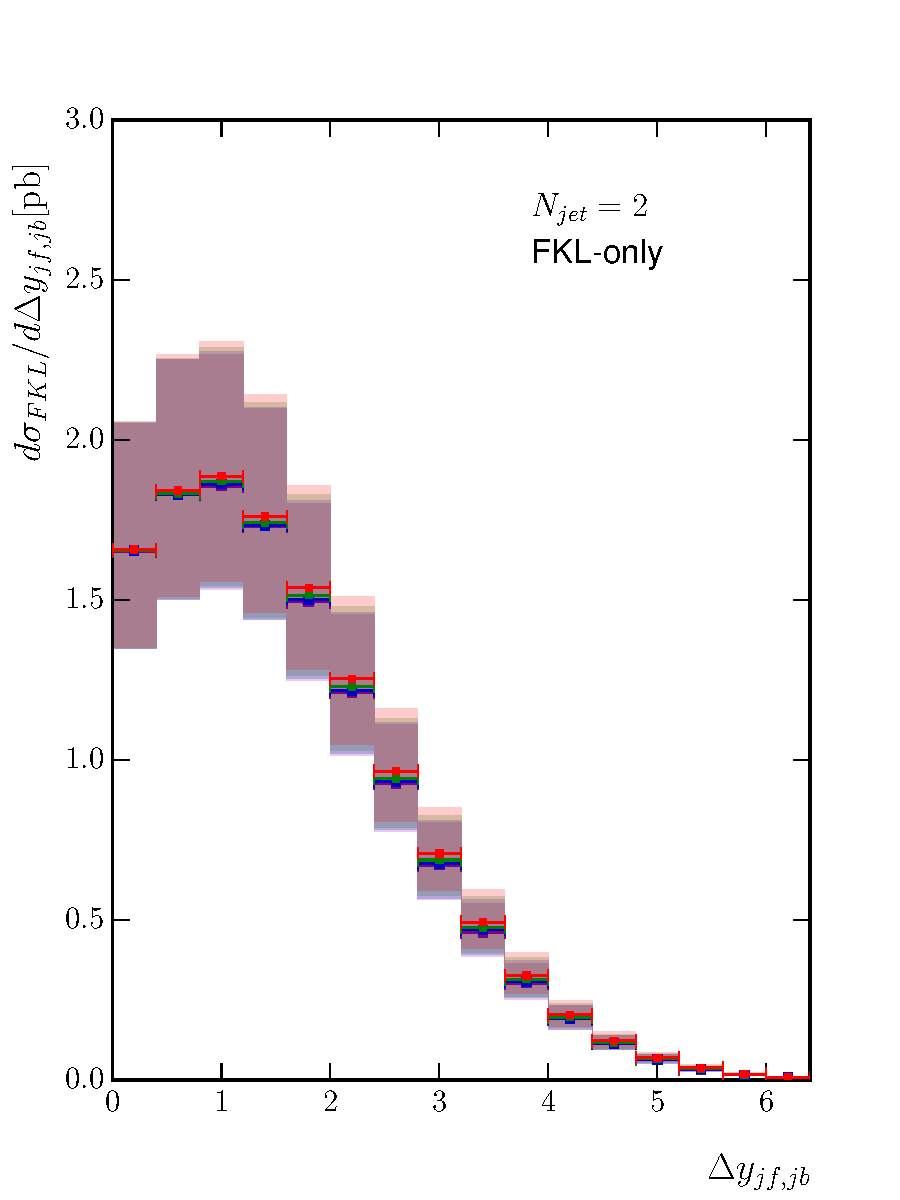
\includegraphics[width=.32\textwidth]{Z_11c_2j.pdf}\hfill
		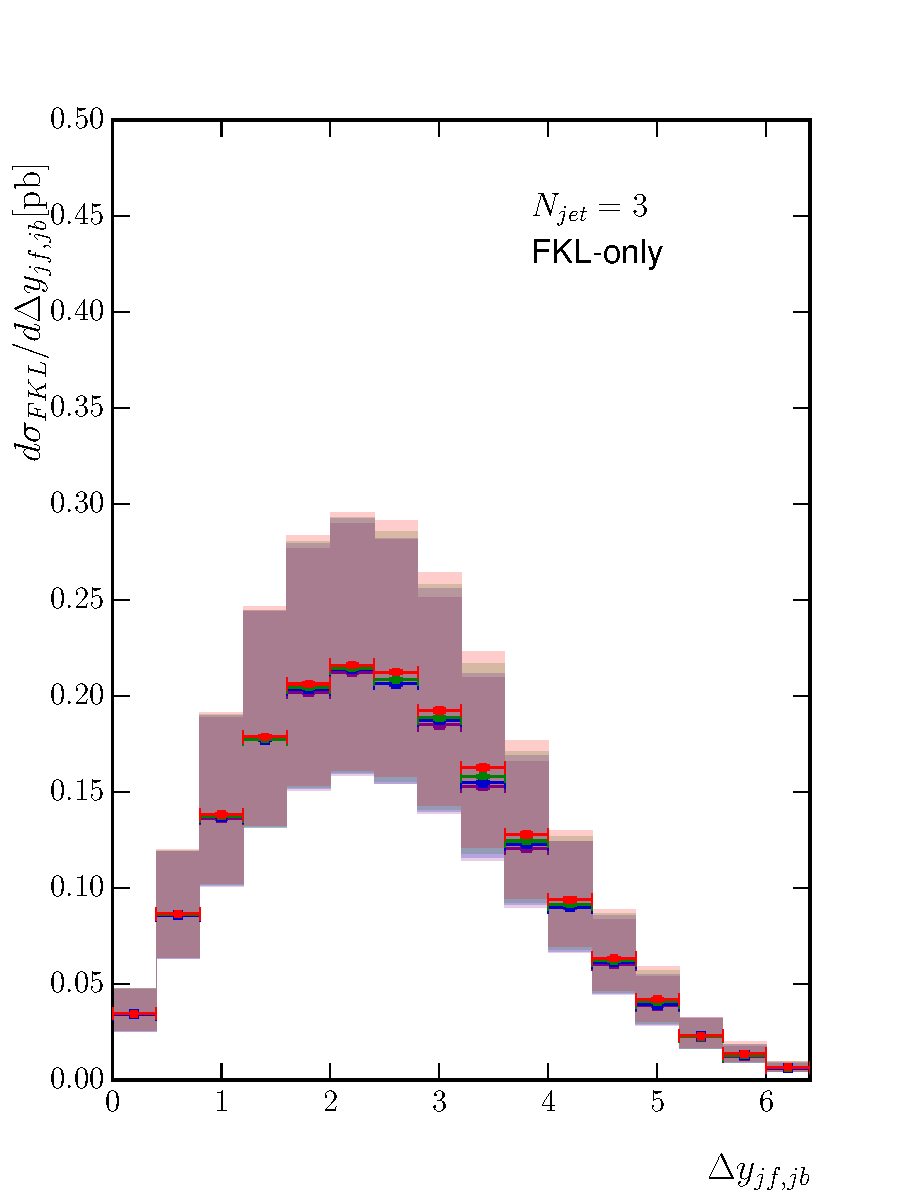
\includegraphics[width=.32\textwidth]{Z_11c_3j.pdf}\hfill
		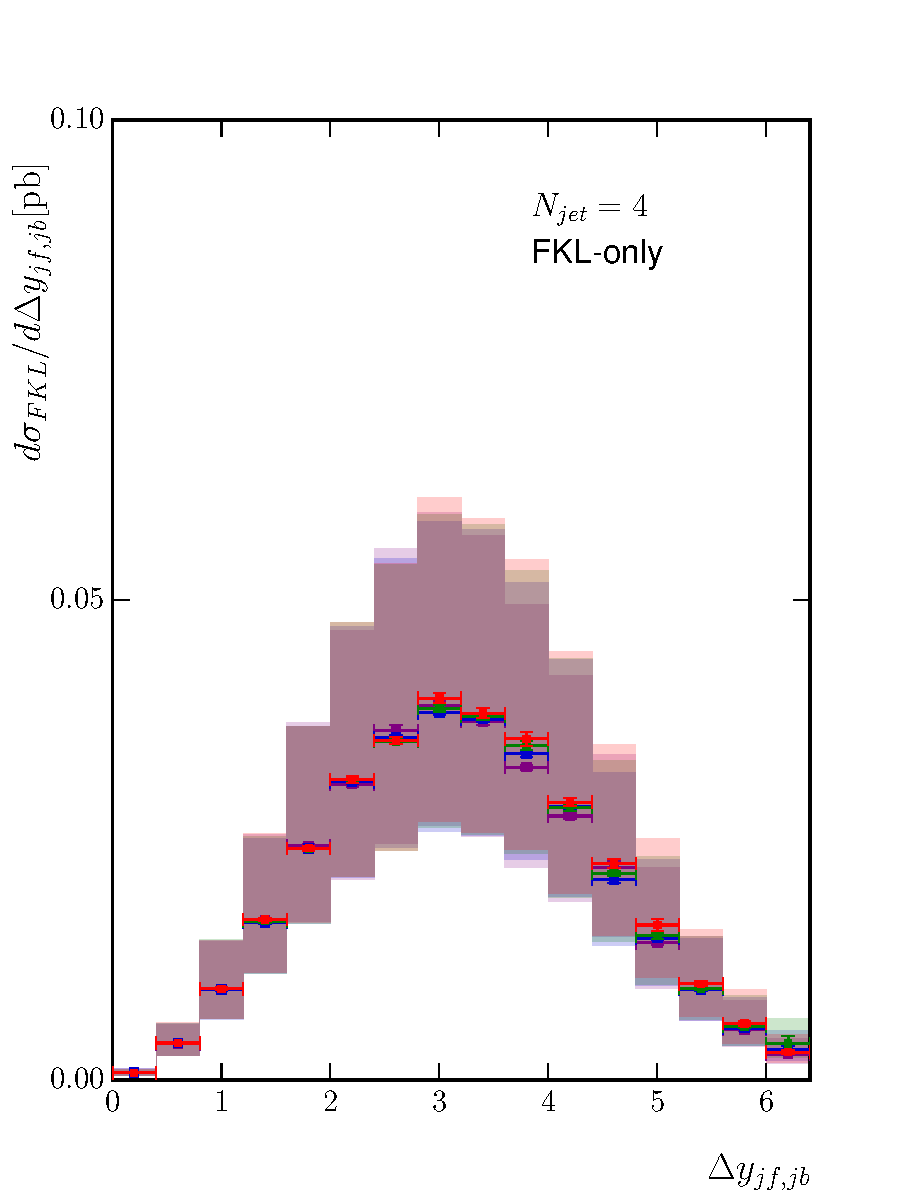
\includegraphics[width=.32\textwidth]{Z_11c_4j.pdf}
		\caption{The effect of varying $\lambda_{cut}$ on the differential distribution
		in the rapidity gap between the two extremal jets in rapidity, $\Delta y_{jf, jb}$,
		with the $N_{jet}=2,3,4$ exclusive selections shown from left to right.
		$\lambda_{cut}=0.2$ (red), 0.5 (blue), 1.0 (green), 2.0 (purple).
		The bands represent the scale variation described in the text.}
		\label{fig:lambdadistdy}
	\end{figure}

\section{The Differential ${Z/\gamma}$ Cross-Section}

	Starting from eqn.~\eqref{eq:allordereg} we can write down a total (differential)
	cross section obtained by summing over all values of the number of final state partons, $n$, and
	integrating over the full $n$-particle phase space using an efficient Monte
	Carlo sampling algorithm~\cite{Andersen:2008ue,Andersen:2008gc}:

	\begin{align}
	  \label{eq:sigma}
	  \begin{split}
	    \sigma =& \sum_{f_a,f_b} \sum_{n=2}^\infty \int \frac{d^3 p_a}{(2\pi)^3 2E_a} \int \frac{d^3
	      p_b}{(2\pi)^3 2E_b}  \left( \prod_{i=1}^n \int \frac{d^3 p_i}{(2\pi)^3
	        2E_i} \right) \int \frac{d^3 p_{e^-}}{(2\pi)^3 2E_{e^-}} \int \frac{d^3 p_{e^+}}{(2\pi)^3 2E_{e^+}} \\
	    & \ \times (2\pi)^4 \delta^{(4)}\left(p_a+p_b -\sum_i p_i - p_{e^-} -p_{e^+}\right) \\
	    & \ \times \ |\mathcal{M}^{HEJ-{\rm reg}}_{f_af_b\to \zg
	      f_a(n-2)gf_b}(p_a,p_b,\{p_i\})|^2 \ \frac{ x_a f_{f_a}(x_a, Q_a) x_b
	      f_{f_b}(x_b,Q_b)}{\hat s^2}\ \Theta_{\rm cut},
	  \end{split}
	\end{align}

	where $x_{a,b}$ are the momentum fractions of the incoming partons and
	$f_{f_k}(x_k,Q_k)$ are the corresponding parton density functions for beam,
	k, and flavour $f_k$.  The function $\Theta_{\rm cut}$ imposes any desired cuts on the final
	state.  The minimum requirement is that the final state momenta cluster into at
	least two jets for the desired jet clustering algorithm.

	In the regions of phase space where all final state particles are well separated
	in rapidity, this gives the dominant terms in QCD at all orders in $\alpha_s$  (the leading logarithmic
	terms in $s/t$).  However, in other areas of
	phase space, the differences due to the approximations used in
	$|\mathcal{M}^{HEJ-{\rm reg}}_{qQ\to \zg q(n-2)gQ}|^2$ will become more
	significant as we saw in figs.~\eqref{fig:ZatLO},~\eqref{fig:3jslice} and~\eqref{fig:4jslice}.
	We can therefore further improve upon eqn.~\eqref{eq:sigma} by
	matching our results to fixed order results.  Here, we match to
	high-multiplicity tree-level
	results obtained from \texttt{MadGraph\_aMC@NLO}~\cite{Alwall:2014hca} in two different ways.
	This amounts to merging tree-level samples of different orders according to the
	logarithmic prescription of HEJ.

	\begin{enumerate}
		\item Matching for FKL configurations:

		  As described in chapter~\ref{chap:HEQCD}, these are the particle assignments
		  and momentum configurations which contain the dominant leading-logarithmic
		  terms in $s/t$.  The first step of the HEJ description was to develop an
		  approximation to the matrix element for these processes which was later
		  supplemented with the finite correction which remained after cancelling the
		  real and virtual divergences: $\overline{|\mathcal{M}_{qg\to Zqg}^{HE}|}^2$
		  (eqn.~(\ref{eq:qgamp})) or $\overline{|\mathcal{M}_{qQ\to ZqQ}^{HE}|}^2$
		  (eqn.~(\ref{eq:allorderreal})).  The approximation is necessary to allow us to
		  describe the matrix element for any (and in particular, large) $n$ and for
		  including both the leading real and virtual corrections.  However,
		  if the parton momenta cluster into four or fewer \emph{jets} (these
		  may have arisen from many more partons), the full tree-level matrix element remains
		  calculable.  In these cases, we perform the matching multiplicatively, so we
		  multiply the integrand of eqn.~(\ref{eq:sigma}) by the ratio:

		  \begin{align}
		    |\mathcal{M}^{\rm full}_{qQ\to \zg q(k-2)gQ}(p_a,p_b,\{
		    j_i'\})|^2/|\mathcal{M}^{HEJ}_{qQ\to \zg q(k-2)gQ}(p_a,p_b,\{j_i'\})|^2.
		  \end{align}

		  Here, $\{j_i'\}$ are the jet momenta after a small amount of
		  reshuffling.  This is necessary because the evaluation of the tree-level matrix elements
		  assumes that the jet momenta are both on-shell and have transverse momenta which
		  sum to zero, neither of which is true in general for our events due to the
		  presence of extra emissions.  Our reshuffling algorithm~\cite{Andersen:2011hs} redistributes this
		  extra transverse momentum in proportion to the size of the transverse
		  momentum of each jet.  The plus and minus light-cone components are then adjusted such
		  that the jet is put on-shell and the rapidity remains unaltered.  This last
		  feature ensures that after reshuffling the event is still in an FKL
		  configuration.

		\item Matching for non-FKL configurations:

		  Away from regions in phase space where the quarks and gluons are
		  well-separated, the non-FKL configurations will play a more significant
		  r\^ole.  These have so far not been accounted for at all, and hence we add
		  three exclusive samples of leading-order two-jet, three-jet and four-jet
		  leading-order events to our resummed events.
	\end{enumerate}

	These two matching schemes complete our description of the production of $\zg$
	with at least two jets, including the leading high-energy logarithms at all
	orders in $\alpha_s$.  Tabs~\eqref{tab:matching1} and~\eqref{tab:matching2} show
	the effect of the matching to leading order on the total cross sections of various FKL
	configurations for 2 and 3-4 jet processes respectively.  We see that although the
	resummation-only result often gives a good approximation to the exact leading order result
	it sometimes differs but that this difference is corrected for by our matching.  Tab.~\eqref{tab:matching3}
	shows the total cross sections generated by \HEJ for 2-, 3- and 4-jet processes which contain non-FKL
	configurations.  Once again we see that after the inclusion of the extra exclusive sums we are in good
	agreement with the leading order result.

	\begin{table}[hbt]
	\centering
	\caption{The effect of matching on the total cross-section of the 2 jet final state FKL configurations.}
	\label{tab:matching1}
	\begin{tabular}{c|c|c|c}
	Incoming & Resum. & Resum.+FKL & Leading Order \\ \hline
	$(1,  1)$       &  $0.6550 \pm 0.0172$  &  $0.6742 \pm 0.0170$  & $0.6742 \pm 0.0170$ \\
	$(1,  2)$       &  $1.1030 \pm 0.0581$  &  $1.1030 \pm 0.0581$  & $1.1029 \pm 0.0581$ \\
	$(1,  3)$       &  $0.2667 \pm 0.0077$  &  $0.2667 \pm 0.0077$  & $0.2667 \pm 0.0077$ \\
	$(1,  4)$       &  $0.1991 \pm 0.0113$  &  $0.1992 \pm 0.0113$  & $0.1992 \pm 0.0113$ \\
	$(1,  5)$       &  $0.1085 \pm 0.0036$  &  $0.1085 \pm 0.0036$  & $0.1085 \pm 0.0036$ \\
	$(2,  2)$       &  $1.3672 \pm 0.0980$  &  $1.3910 \pm 0.0935$  & $1.3910 \pm 0.0935$ \\
	$(2,  3)$       &  $0.4832 \pm 0.0174$  &  $0.4832 \pm 0.0174$  & $0.4832 \pm 0.0174$ \\
	$(2,  4)$       &  $0.2744 \pm 0.0203$  &  $0.2744 \pm 0.0203$  & $0.2744 \pm 0.0203$ \\
	$(2,  5)$       &  $0.2033 \pm 0.0082$  &  $0.2033 \pm 0.0082$  & $0.2033 \pm 0.0082$ \\
	$(3,  3)$       &  $0.0837 \pm 0.0021$  &  $0.0880 \pm 0.0022$  & $0.0880 \pm 0.0022$ \\
	$(3,  4)$       &  $0.0630 \pm 0.0034$  &  $0.0630 \pm 0.0034$  & $0.0630 \pm 0.0034$ \\
	$(3,  5)$       &  $0.0313 \pm 0.0008$  &  $0.0313 \pm 0.0008$  & $0.0313 \pm 0.0008$ \\
	$(4,  4)$       &  $0.0310 \pm 0.0018$  &  $0.0326 \pm 0.0017$  & $0.0326 \pm 0.0017$ \\
	$(4,  5)$       &  $0.0236 \pm 0.0016$  &  $0.0236 \pm 0.0016$  & $0.0236 \pm 0.0016$ \\
	$(5,  5)$       &  $0.0114 \pm 0.0003$  &  $0.0121 \pm 0.0003$  & $0.0121 \pm 0.0003$ \\
	$(1, 21)$       &  $4.3680 \pm 0.1600$  &  $2.7868 \pm 0.0909$  & $2.7868 \pm 0.0909$ \\
	$(2, 21)$       &  $5.6100 \pm 0.3344$  &  $3.6284 \pm 0.1957$  & $3.6284 \pm 0.1957$ \\
	$(3, 21)$       &  $1.8842 \pm 0.0732$  &  $1.1718 \pm 0.0353$  & $1.1718 \pm 0.0353$ \\
	$(4, 21)$       &  $1.2172 \pm 0.1449$  &  $0.7136 \pm 0.0405$  & $0.7136 \pm 0.0405$ \\
	$(5, 21)$       &  $0.7480 \pm 0.0335$  &  $0.4697 \pm 0.0153$  & $0.4697 \pm 0.0153$ \\ \hline
	\end{tabular}
	\end{table}

	\begin{table}[hbt]
	\centering
	\caption{The effect of matching on the total cross-section of the 3 and 4 jet final state FKL
	configurations.}
	\label{tab:matching2}
	\begin{tabular}{c|c|c}
	Incoming & Resum.+FKL & Leading Order \\ \hline
	\multicolumn{3}{c}{3-jet} \\ \hline
	$(1, 1)$  & $0.3467 \pm 0.0202$ & $0.3467 \pm 0.0202$ \\
	$(1, 2)$  & $0.6851 \pm 0.0589$ & $0.6851 \pm 0.0589$ \\
	$(1, 3)$  & $0.1065 \pm 0.0073$ & $0.1065 \pm 0.0073$ \\
	$(1, 4)$  & $0.0684 \pm 0.0059$ & $0.0684 \pm 0.0059$ \\
	$(1, 5)$  & $0.0431 \pm 0.0032$ & $0.0431 \pm 0.0032$ \\ \hline
	\multicolumn{3}{c}{4-jet} \\ \hline
	$(3, 1)$  & $0.0011 \pm 0.0001$ & $0.0011 \pm 0.0001$ \\
	$(3, 5)$  & $0.0097 \pm 0.0006$ & $0.0097 \pm 0.0006$ \\ \hline
	\end{tabular}
	\end{table}

	\begin{table}[hbt]
	\centering
	\caption{The effect of matching on the total cross-section of the 2-, 3- and 4-jet final state non-FKL
	configurations.}
	\label{tab:matching3}
	\begin{tabular}{c|c|c|c|c}
	Incoming & Resum.+FKL & Non-FKL & Leading Order & \HEJ/Leading Order\\ \hline
	\multicolumn{5}{c}{2-jet} \\ \hline
	$(1, 2)$    &   $1.0985 \pm 0.1048$ &   $0.1047 \pm 0.0072$ &   $1.2260  \pm 0.0037$ & $0.9814  \pm 0.0857$ \\
	$(3, 4)$    &   $0.0706 \pm 0.0107$ &   $0.0086 \pm 0.0001$ &   $0.0804  \pm 0.0001$ & $0.98587 \pm 0.1334$ \\
	$(21, 21)$  &   $0.0000 \pm 0.0000$ &   $0.4002 \pm 0.9090$ &   $0.3612  \pm 0.0357$ & $1.00389 \pm 0.0878$ \\
	$(1,-1)$    &   $0.4262 \pm 0.0107$ &   $1.8962 \pm 0.0586$ &   $2.3460  \pm 0.0064$ & $0.98991 \pm 0.0255$ \\
	$(2,-2)$    &   $0.6151 \pm 0.0640$ &   $2.0954 \pm 0.0742$ &   $2.6770  \pm 0.0079$ & $1.01254 \pm 0.0367$ \\
	$(3,-3)$    &   $0.1250 \pm 0.0154$ &   $0.6116 \pm 0.0078$ &   $0.7576  \pm 0.0023$ & $0.97232 \pm 0.0230$ \\
	$(4,-4)$    &   $0.0733 \pm 0.0319$ &   $0.2308 \pm 0.0040$ &   $0.3096  \pm 0.0010$ & $0.98228 \pm 0.1037$ \\
	$(5,-5)$    &   $0.0186 \pm 0.0003$ &   $0.1211 \pm 0.0036$ &   $0.1447  \pm 0.0005$ & $0.96592 \pm 0.0254$ \\ \hline
	\multicolumn{5}{c}{3-jet} \\ \hline
        $(1,-1)$    &   $0.1713 \pm 0.0026$ &   $0.4848 \pm 0.0104$ &   $0.6112  \pm 0.0031$ & $1.0354 \pm 0.0183$ \\
        $(21, 21)$  &   $0.0000 \pm 0.0000$ &   $6.8566 \pm 0.2022$ &   $6.7920  \pm 0.0220$ & $1.0095 \pm 0.0299$ \\
        $(3, 1)$    &   $0.0008 \pm 0.0000$ &   $0.1615 \pm 0.0041$ &   $0.1633  \pm 0.0005$ & $0.9937 \pm 0.9937$ \\
        $(2,-5)$    &   $0.0724 \pm 0.0053$ &   $0.0627 \pm 0.0046$ &   $0.1300  \pm 0.0005$ & $1.0392 \pm 0.0544$ \\
        $(1, 21)$   &   $0.5804 \pm 0.0930$ &   $3.4127 \pm 0.2900$ &   $4.1498  \pm 0.0149$ & $0.9624 \pm 0.0735$ \\ \hline
	\multicolumn{5}{c}{4-jet} \\ \hline
	$(1, 2)$   &    $0.2308 \pm 0.0230$ &   $0.3199 \pm 0.0447$ &   $0.5491 \pm 0.0032$  & $1.0030 \pm 0.0917$ \\
	$(4, 21)$  &    $0.0133 \pm 0.0007$ &   $0.2728 \pm 0.0370$ &   $0.2780 \pm 0.0509$  & $1.0292 \pm 0.1334$ \\
	$(1,-1)$   &    $0.0545 \pm 0.0030$ &   $0.1544 \pm 0.0111$ &   $0.1965 \pm 0.0011$  & $1.0631 \pm 0.0588$ \\
	$(3,-3)$   &    $0.0002 \pm 0.0000$ &   $0.0366 \pm 0.0042$ &   $0.0333 \pm 0.0001$  & $1.1059 \pm 0.1251$ \\ \hline
	\end{tabular}
	\end{table}

	In the next sections, we discuss the computational aspects of the work presented
	here and compare the resulting predictions from this formalism to LHC data from
	recent ATLAS and CMS analyses.

\section{$\zg$+Jets: Computational Aspects}
	\label{sec:comp}

	The physics presented in the preceding sections is a significant departure from
	work previously done by the High Energy Jets collaboration.  As such developing
	the Monte Carlo for $\zg$ plus jets was a serious undertaking; the inclusion of
	the aforementioned interference terms required that two $t$-channel `chains' of
	momenta and vertices be computed and carried throughout the evaluation.
	Furthermore to correctly calculate at the amplitude level the way the \hej currents
	are constructed in the codebase needed to be modified.  Since the virtual corrections
	are scale dependent it was necessary to change large sections of code to work with
	multiple copies of $t$-chains and multiple scales.

	In previous \HEJ releases the matching mentioned above was performed using
	\texttt{MadGraph} version 4.  However, due to increases in speed and efficiency
	we chose to match the $\zg$+jets \HEJ matrix elements to \texttt{MadGraph\_aMC@NLO} version 5.
	While this might seem like a trivial change the underlying computational work
	was anything but simple; since the latest version of \texttt{MadGraph} outputs
	matrix elements in C++ (as well as Fortran 90) a completely new approach
	to incorporating matching was required.  A novel `abstract factory' design pattern
	was employed to efficiently construct and call the relevant leading order
	matrix element.  In this way we avoided the necessity of having extremely large
	matching files containing $\mathcal{O}(18,000)$ lines of code which was very difficult to
	debug and improve; instead this new structure allowed the matching code to
	be reduced to only a few thousand lines since the abstract factory class
	presents a uniform interface and therefore almost all of the process specific
	lines became unnecessary (some process specific content remains due to the
	distinction made between FKL and non-FKL configurations).

	Throughout the course of this work it became apparent that the \hej
	codebase as it was at the time needed to be restructured.  Each physics
	process (pure jets, $W^\pm$+jets, Higgs+jets and $\zg$+jets) was structured
	individually as a stand-alone piece of code.  This became a problem when testing
	and modifying \HEJ since there are large sections of code which are the same
	regardless of what electroweak boson emission (if any) we are concerned with,
	for example the parton distribution function calls are almost entirely the same
	no matter which code is run.  To improve upon this situation a unified \HEJ
	package was created.  This was a complete restructuring of the code into a form
	in which a general \texttt{HejGen} polymorphic base class can be
	constructed abstractly and then made concrete depending on user input.
	The unified version of the code is an improvement in that it is much more user
	friendly, and significantly easier to test and extend.  This work entailed
	being one of the primary authors of the new design for \hej and will soon be
	released as \HEJ (v2).

	Lastly a word about the generation of \hej predictions for comparisons to data.
	The sections and chapters which follow contain theoretical predictions to
	experimental analyses.  These predictions were generated using distributed
	computing both locally in Edinburgh and using the CERN \texttt{GRID} system.
	The former required the development of a set-up to distribute, execute and
	finalise jobs across a large network of machines standard desktop machines (i.e.~not
	actual computing nodes) distributed through Edinburgh University.  This was
	a time-consuming process however without this system it would not have been
	possible to produce the interesting results of chapter~\ref{chap:ATLAS} (which
	also contains a discussion of the computational challenges of generating \HEJA
	predictions). The \texttt{GRID} distributed computing work was available only in
	the final stages of this work because it became clear it was necessary (had it
	been available sooner the aforementioned local distributed computing set-up could
	have been avoided completely).  This involved a good deal of learning to work with
	distributed systems and working with the \texttt{Ganga} batch submission
	system which was, again, time-consuming.

\section{$\zg$+Jets at the LHC}

	\subsection{$\zg$+Jets at the ATLAS Experiment}
		\label{sub:ATLASZsec}

		We now compare the results of the formalism described in the previous sections
		to data.  We begin with a recent ATLAS analysis of $Z^0$-plus-jets events from
		7~TeV collisions~\cite{Aad:2013ysa}.  We summarise the cuts in tab.~\eqref{tab:atlascuts}.

		Any jet which failed the final isolation cut was removed from the event, but the
		event itself is kept provided there are a sufficient number of other jets
		present.  Throughout the central value of the \texttt{HEJ} predictions has been
		calculated with factorisation and renormalisation scales set to
		$\mu_F=\mu_R=H_T/2$, and the theoretical uncertainty band has been determined by
		varying these independently by up to a factor of 2 in each direction (removing
		the corners where the relative ratio is greater than two).  Also shown in the
		plots taken from the ATLAS paper are theory predictions from
		\texttt{Alpgen}~\cite{Mangano:2002ea}, \texttt{Sherpa}~\cite{Gleisberg:2008ta,Hoeche:2012yf},
		\texttt{MC@NLO}~\cite{Frixione:2002ik} and
		\texttt{BlackHat+Sherpa}~\cite{Berger:2010vm,Ita:2011wn}.  We will also comment on the
		recent theory description of Ref.\cite{Frederix:2015eii} .

		In Fig.~\eqref{fig:ATLAS_2a}, we begin this set of comparisons with predictions
		and measurements of the inclusive jet rates.  \texttt{HEJ} and most of the other theory
		descriptions give a reasonable description of these rates.  The \texttt{MC@NLO}
		prediction drops below the data because it only contains the hard-scattering
		matrix element for $\zg$ production and relies on a parton shower for additional
		emissions. The \texttt{HEJ} predictions have a larger uncertainty band which largely
		arises from the use of leading-order results in the matching procedures.

		The first differential distribution we consider here is the distribution of the
		invariant mass between the two hardest jets, Fig.~\eqref{fig:ATLAS_11b}.  The
		region of large invariant mass is particularly important because this is a
		critical region for studies of vector boson fusion (VBF) processes in
		Higgs-plus-dijets.  Radiation patterns are largely universal between these
		processes, so one can test the quality of theoretical descriptions in
		$\zg$-plus-dijets and use these to inform the VBF analyses.  It is also a
		distribution which will be studied to try to detect subtle signs of new physics.
		In this study, \texttt{HEJ} and the other theory descriptions all give a good description
		of this variable out to 1~TeV, with \texttt{HEJ} being closest throughout the range.  The
		merged sample of Ref.~\cite{Frederix:2015eii} (Fig.~9 in that paper) combined
		with the \texttt{Pythia8} parton shower performs reasonably well throughout the range
		with a few deviations of more than 20\%, while that combined with \texttt{Herwig++}
		deviates badly.  Fig.~\eqref{fig:wJetsEg} shows the equivalent distribution from
		a recent ATLAS analysis of $W^\pm$+dijet events~\cite{Aad:2014qxa}, that distribution
		was extended out to an invariant mass of $2$~TeV and, as discussed in section~\ref{sec:HEJ},
		almost all of the theoretical predictions deviated significantly while the \texttt{HEJ}
		prediction remained flat.  This is one region where the high-energy logarithms
		which are only included in \texttt{HEJ} are expected to become large.

		In Fig.~\eqref{fig:ATLAS_11a}, we show the comparison of various theoretical
		predictions to the distribution of the absolute rapidity difference between the
		two leading jets.  It is clear in the left plot that \texttt{HEJ} gives an excellent
		description of this distribution.  This is to some extent expected as
		high-energy logarithms are associated with rapidity separations.  However, this
		variable is only the rapidity separation between the two hardest jets which is
		often not representative of the event as harder jets tend to be more central.
		Nonetheless, the \texttt{HEJ} description performs well in this restricted scenario.  The
		next-to-leading order (NLO) calculation of \texttt{Blackhat+Sherpa} also describes the
		distribution quite well while the other merged, fixed-order samples deviate from
		the data at larger values.  The merged samples of Ref.~\cite{Frederix:2015eii}
		(Fig.~8 in that paper) describe this distribution well for small values of this
		variable up to about 3 units when combined with \texttt{Herwig++} and for most of the
		range when combined with the \texttt{Pythia8} parton shower, only deviating above 5 units.

		The final distribution in this section is that of the ratio of the transverse
		momentum of the second hardest jet to the hardest jet.  The perturbative
		description of \texttt{HEJ} does not contain any systematic evolution of transverse
		momentum and this can be seen where its prediction undershoots the data at low
		values of $p_{T2}/p_{T1}$.  However, for values of $p_{T2} \gtrsim 0.5 p_{T1}$,
		the ratio of the \texttt{HEJ} prediction to data is extremely close to 1.  The
		fixed-order based predictions shown in Fig.~\eqref{fig:ATLAS_2a} are all fairly
		flat above about 0.2, but the ratio of the data differs by about 10\%.

		We have seen that in all of the figures presented in this section \HEJ has scale uncertainty bands
		significantly larger than other theoretical descriptions, including \texttt{Alpgen} who also
		have only leading order accuracy.  From fig.~\eqref{fig:ATLAS_2a} we see that we describe
		the experimentally observed inclusive two jet rate very well and, as such, do not require
		normalisation to agree with the data.  However, applying a normalisation procedure which
		consistently applies scale variation simultaneously in numerator and denominator significantly
		reduces the size of the scale uncertainty bands for High Energy Jets (or any theoretical prediction).
		In figs.~\eqref{fig:ATLAS_Z_7b_norm},~\eqref{fig:ATLAS_Z_11a_norm} and~\eqref{fig:ATLAS_Z_11b_norm}
		we show the results from figs.~\eqref{fig:HEJ_ATLAS_7b},~\eqref{fig:HEJ_ATLAS_11a} and~\eqref{fig:HEJ_ATLAS_11b}.
		We see that, as expected, the central value of HEJ still describes the data well in the
		regions discussed above and now the size of the theoretical uncertainty band is significantly
		reduced (by a factor of around 250 for example in the last bin of the
		$p_{\perp 2}/p_{\perp 1}$-distribution.  This illustrates that varying $\mu_R$ and $\mu_F$
		leads to a change in overall normalisation but not to any significant change in shape.  Therefore,
		it is still valuable to discuss the quality of agreement of the central line, despite their
		apparently large accompanying uncertainty bands.

		\begin{table}[bth]
		  \centering
		  \begin{tabular}{|l|c|}
		    \hline
		    Lepton Cuts & $p_{T\ell}>20$~GeV, \; $|\eta_\ell|<2.5$ \\
		    & $\Delta R^{\ell^+\ell^-} > 0.2$, \; $66$~GeV $\leq m^{\ell^+\ell^-} \leq
		      116$~GeV \\ \hline
		    Jet Cuts (anti-$k_T$, 0.4) & $p_{Tj}>30$~GeV, \; $|y_j|<4.4$ \\
		    & $\Delta R^{j\ell} >0.5$ \\
		\hline
		  \end{tabular}
		  \caption{Cuts applied to theory simulations in the ATLAS
		    $Z^0$-plus-jets analysis results shown in Figs.~\eqref{fig:ATLAS_2a}--\eqref{fig:ATLAS_7b}.}
		  \label{tab:atlascuts}
		\end{table}

		\begin{figure}[H]
		  \centering
		  \begin{subfigure}[b]{0.48\textwidth}
		    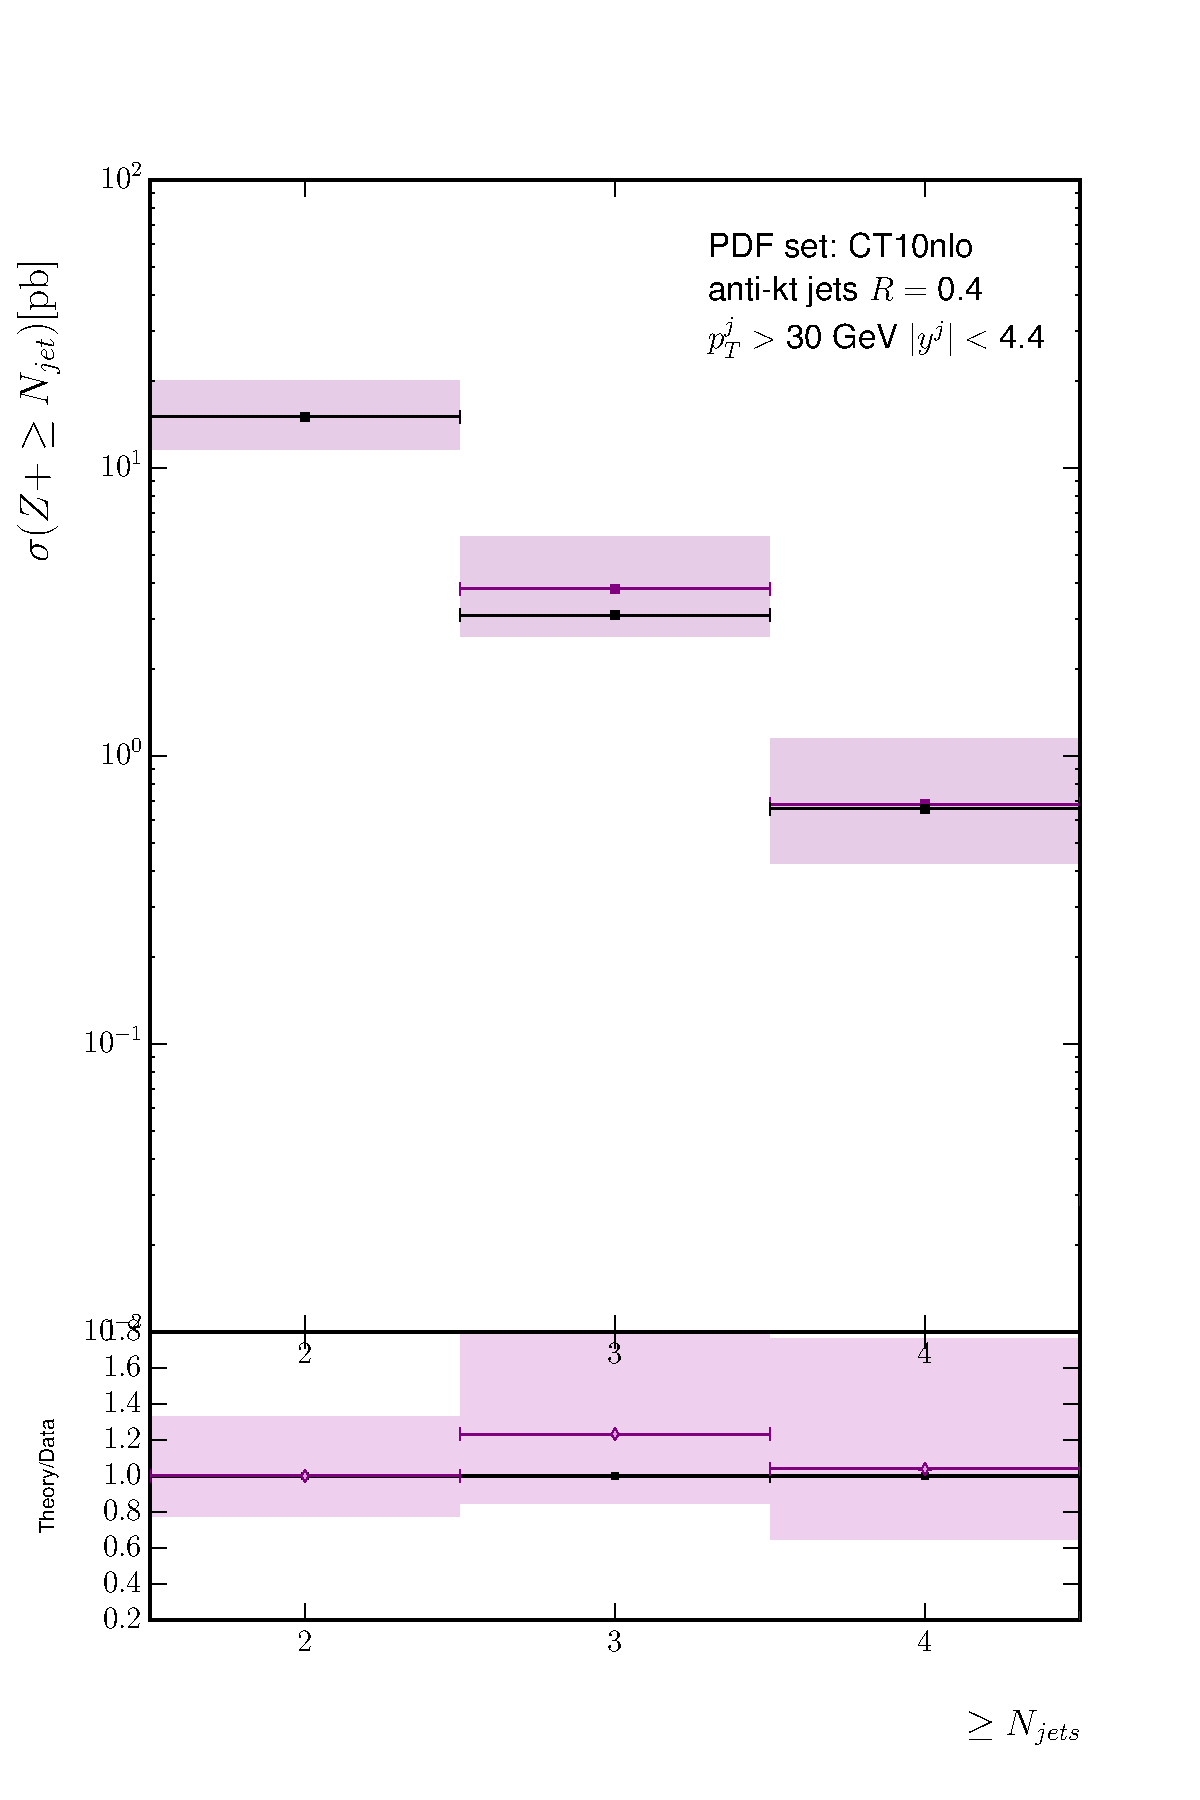
\includegraphics[width=\textwidth, height=1.2\textwidth]{ATLAS_Z_2a}
		    \label{fig:HEJ_ATLAS_2a}
		  \end{subfigure}
		  ~
		  \begin{subfigure}[b]{0.48\textwidth}
		    \includegraphics[width=\textwidth, height=1.2\textwidth]{Comparison_2a}
		    \caption{}
		    \label{fig:MC_ATLAS_2a}
		  \end{subfigure}
		  \caption{These plots show the inclusive jet rates from (a) \texttt{HEJ} and (b) other
		    theory descriptions and data~\cite{Aad:2013ysa}.  \texttt{HEJ} events all contain at
		    least two jets and do not contain matching for 5 jets and above, so these
		    bins are not shown.}
		  \label{fig:ATLAS_2a}

		  \begin{subfigure}[b]{0.48\textwidth}
		    \includegraphics[width=\textwidth, height=1.2\textwidth]{ATLAS_Z_11b}
		    \caption{}
		    \label{fig:HEJ_ATLAS_11b}
		  \end{subfigure}
		  ~
		  \begin{subfigure}[b]{0.48\textwidth}
		    \includegraphics[width=\textwidth, height=1.2\textwidth]{Comparison_11b}
		    \caption{}
		    \label{fig:MC_ATLAS_11b}
		  \end{subfigure}
		  \caption{These plots show the invariant mass between the leading and
		    second-leading jet in $p_T$.  As in Fig.~\eqref{fig:ATLAS_2a}, predictions are
		    shown from (a) \texttt{HEJ} and (b) other theory descriptions and
		    data~\cite{Aad:2013ysa}. These studies will inform Higgs plus dijets
		    analyses, where cuts are usually applied to select events with large
		    $m_{12}$.}
		  \label{fig:ATLAS_11b}
		\end{figure}

		\begin{figure}[H]
		  \centering
		  \begin{subfigure}[b]{0.48\textwidth}
		    \includegraphics[width=\textwidth, height=1.2\textwidth]{ATLAS_Z_11a}
		    \caption{}
		    \label{fig:HEJ_ATLAS_11a}
		  \end{subfigure}
		  ~
		  \begin{subfigure}[b]{0.48\textwidth}
		    \includegraphics[width=\textwidth, height=1.2\textwidth]{Comparison_11a}
		    \caption{}
		    \label{fig:MC_ATLAS_11a}
		  \end{subfigure}
		  \caption{The comparison of (a) \texttt{HEJ} and (b) other theoretical descriptions and
		    data~\cite{Aad:2013ysa} to
		    the distribution of the absolute rapidity different between the two leading
		    jets.  \texttt{HEJ} and \texttt{Blackhat+Sherpa} give the best description.}
		  \label{fig:ATLAS_11a}

		  \begin{subfigure}[b]{0.48\textwidth}
		    \includegraphics[width=\textwidth, height=1.2\textwidth]{ATLAS_Z_7b}
		    \caption{}
		    \label{fig:HEJ_ATLAS_7b}
		  \end{subfigure}
		  ~
		  \begin{subfigure}[b]{0.48\textwidth}
		    \includegraphics[width=\textwidth, height=1.2\textwidth]{Comparison_7b}
		    \caption{}
		    \label{fig:MC_ATLAS_7b}
		  \end{subfigure}
		  \caption{These plots show the differential cross section in the ratio of the leading
		     and second leading jet in $p_T$ from (a) \texttt{HEJ} and (b) other
		    theory descriptions and data~\cite{Aad:2013ysa}.}
		  \label{fig:ATLAS_7b}
		\end{figure}

		\begin{figure}[H]

			\centering

			\begin{subfigure}[b]{0.48\textwidth}
			  \includegraphics[width=0.9\textwidth]{ATLAS_Z_7b_norm}
			  \vspace{0.2cm}
			  \caption{}
			  \label{fig:ATLAS_Z_7b_norm}
			\end{subfigure}

			\begin{subfigure}[b]{0.48\textwidth}
			  \includegraphics[width=0.9\textwidth]{ATLAS_Z_11a_norm}
			  \vspace{0.2cm}
			  \caption{}
			  \label{fig:ATLAS_Z_11a_norm}
			\end{subfigure}
			~
			\begin{subfigure}[b]{0.48\textwidth}
			  \includegraphics[width=0.96\textwidth]{ATLAS_Z_11b_norm}
			  \caption{}
			  \label{fig:ATLAS_Z_11b_norm}
			\end{subfigure}
			\caption{The predictions of figs.~\eqref{fig:HEJ_ATLAS_7b},~\eqref{fig:HEJ_ATLAS_11a} and~\eqref{fig:HEJ_ATLAS_11b}
			normalised to the total cross-section, with scale variation consistently applied to numerator and denominator.}

			\label{fig:ATLAS_norm}
		\end{figure}

	\subsection{The $W^\pm$+Jets to $\zg$+Jets Ratio at the ATLAS Experiment}
		\label{sub:ATLASWZsec}

		In this section we present predictions for the ratio of $\zg$+Jets to
		$W^\pm$+Jets at all orders in $\alpha_s$.  We compare to the recent study undertaken
		by the ATLAS collaboration~\cite{Aad:2014rta}.  While $W^\pm$ plus jets and $\zg$ plus
		jets are both relevant separately for Standard Model physics and beyond the ratio of
		the two processes is particularly interesting as a precision test since many of the
		systematic errors which limit the $W^\pm, \zg$-plus-jets measurements cancel in the
		ratio.  The cuts for both final states are summarised in tab.~\eqref{tab:atlasWZcuts}.

		\begin{table}[h]
		\centering
		\begin{tabular}{|l|l|}
			\hline
			Lepton Cuts & $p_{T\ell}>25$~GeV, \; $|\eta_\ell|<2.5$ \\
			&  $\Delta R^{\ell^+\ell^-} > 0.2$ \\ \hline
			Reconstructed $Z$ Cuts &  $66$~GeV $< m^{\ell^+\ell^-} <116$~GeV \\
			\hline
			Reconstructed $W^\pm$ Cuts & $m_{TW} > 40$~GeV\; $\slashed E_{T} > 25$~GeV \\ \hline
			Jet Cuts (anti-$k_T$, 0.4) & $p_{Tj}>30$~GeV, \; $|y_j|<4.4$ \\
			& $\Delta R^{j\ell} >0.5$ \\
			\hline
			\end{tabular}
			\caption{Cuts applied to theory simulations in the analysis of the ATLAS $W^\pm$+jets/$Z$+jets ratio
		  	predictions shown in tabs.~\eqref{tab:RJetsIncl}--\eqref{tab:RJetsExcl}.}
			\label{tab:atlasWZcuts}
		\end{table}

		\begin{table}[!h]
			\begin{center}
			\begin{tabular}{| c | c | c | c |}
		        \hline
			$N_{jets}$ & Data $(\pm \text{stat.}\pm \text{syst.})$ & HEJ $(\pm \text{stat.}\pm \text{s.v.})$ & HEJ/Data $(\pm \text{stat.}\pm \text{s.v.})$ \\ \hline
			$\ge2$ & $8.64\pm0.04\pm0.33$ & $8.66\pm0.12^{+0.14}_{-0.16}$ & $1.00\pm0.01^{+0.02}_{-0.01}$ \\ \hline
			$\ge3$ & $8.18\pm0.08\pm0.52$ & $7.96\pm0.25^{+0.01}_{-0.01}$ & $0.97\pm0.03^{+0.01}_{-0.00}$ \\ \hline
			$\ge4$ & $7.62\pm0.20\pm0.95$ & $8.55\pm0.69^{+0.02}_{-0.02}$ & $1.12\pm0.09^{+0.00}_{-0.00}$ \\ \hline
			\end{tabular}
			\caption{The HEJ prediction for inclusive $R_{jet}$ rates at 2, 3 and 4 jets compared with ATLAS data.}
			\label{tab:RJetsIncl}
			\end{center}
		\end{table}

		\begin{table}[!h]
			\begin{center}
			\begin{tabular}{| c | c | c | c |}
		        \hline
			$N_{jets}$ & Data $(\pm \text{stat.}\pm \text{syst.})$ & HEJ $(\pm \text{stat.}\pm \text{s.v.})$ & HEJ/Data $(\pm \text{stat.}\pm \text{s.v.})$ \\ \hline
			2 & $8.76\pm0.05\pm0.31$ & $8.88\pm0.135^{+0.15}_{-0.18}$ & $1.01\pm0.02^{+0.021}_{-0.02}$ \\ \hline
			3 & $8.33\pm0.10\pm0.45$ & $7.85\pm0.265^{+0.01}_{-0.01}$ & $0.94\pm0.01^{+0.001}_{-0.03}$ \\ \hline
			4 & $7.69\pm0.21\pm0.71$ & $8.44\pm0.684^{+0.04}_{-0.04}$ & $1.10\pm0.01^{+0.005}_{-0.09}$ \\ \hline
			\end{tabular}
			\caption{The HEJ prediction for exclusive $R_{jet}$ rates at 2, 3 and 4 jets compared with ATLAS data.}
			\label{tab:RJetsExcl}
			\end{center}
		\end{table}

	\subsection{$\zg$+Jets at the CMS Experiment}
		\label{sub:CMS}

		We now compare to data from a CMS analysis of events with a $\zg$ boson produced
		in association with jets~\cite{Khachatryan:2014zya}.  We show, for comparison,
		the plots from that analysis which contain theoretical predictions from
		Sherpa~\cite{Gleisberg:2008ta,Hoeche:2012yf}, \texttt{Powheg}~\cite{Alioli:2010qp} and
		\texttt{MadGraph\_aMC@NLO}~\cite{Alwall:2014hca}.The cuts used for this analysis are summarised in
		tab.~\eqref{tab:cmscuts}.

		\begin{table}[hbt]
		  \centering
		  \begin{tabular}{|l|c|}
		    \hline
		    Lepton Cuts & $p_{T\ell}>20$~GeV, \; $|\eta_\ell|<2.4$ \\
		    &\; $71$~GeV $\leq m^{\ell^+\ell^-} \leq
		      111$~GeV \\ \hline
		    Jet Cuts (anti-$k_T$, 0.5) & $p_{Tj}>30$~GeV, \; $|y_j|<2.4$ \\
		    & $\Delta R^{j\ell} >0.5$ \\
		\hline
		  \end{tabular}
		  \caption{Cuts applied to theory simulations in the CMS
		    $Z^0$-plus-jets analysis results shown in
		    Figs.~\eqref{fig:CMS_2a}--\eqref{fig:CMS_3c}}
		  \label{tab:cmscuts}
		\end{table}

		As in the previous section, any jet which failed the final isolation cut was
		removed from the event, but the event itself is kept provided there are a
		sufficient number of other jets present.  The main difference to these cuts and
		those of ATLAS in the previous section is that the jets are required to be more
		central; $|\eta|<2.4$ as opposed to $|y|<4.4$.  This allows less room for
		evolution in rapidity; however, \texttt{HEJ} predictions are still relevant in this
		scenario.  Once again, the central values are given by $\mu_F=\mu_R=H_T/2$ with
		theoretical uncertainty bands determined by varying these independently by
		factors of two around this value.  \texttt{HEJ} events always contain a minimum of two
		jets and therefore here we only compare to the distributions for an event sample
		with at least two jets or above.

		We begin in Fig.~\eqref{fig:CMS_2a} by showing the inclusive jet rates for these
		cuts.  The \texttt{HEJ} predictions give a good description, especially for the 2- and
		3-jet inclusive rates in this narrower phase space. The uncertainty bands are
		larger for \texttt{HEJ} than for the \texttt{Sherpa} and \texttt{Powheg} predictions
		due to our LO matching prescription (those for \texttt{MadGraph\_aMC@NLO} are not shown).

		In Figs.~\eqref{fig:CMS_3b}--~\eqref{fig:CMS_3c}, we show the transverse momentum
		distributions for the second and third jet respectively (the leading jet
		distribution was not given for inclusive dijet events).  Beginning with the
		second jet in Fig.~\eqref{fig:CMS_3b}, we see that the \texttt{HEJ} predictions overshoot
		the data at large transverse momentum.  In this region, the non-FKL matched
		components of the \texttt{HEJ} description become more important and these are not
		controlled by the high-energy resummation.  The \texttt{HEJ} predictions are broadly
		similar to \texttt{Powheg}'s $Z^0$-plus-one-jet NLO calculation matched with the Pythia
		parton shower.  In contrast, \texttt{Sherpa}'s prediction significantly undershoots the
		data at large transverse momentum.  Here the \texttt{MadGraph\_aMC@NLO} prediction gives the best
		description of the data.

		Fig.~\eqref{fig:CMS_3c} shows the transverse momentum distribution of the third
		jet in this data sample.  Here, the ratio of the \texttt{HEJ} prediction to data shows a
		linear increase with transverse momentum (until the last bin where all the
		theory predictions show the same dip).  Both the \texttt{Sherpa} and \texttt{Powheg} predictions
		show similar deviations for this variable while the \texttt{MadGraph\_aMC@NLO} prediction again
		performs very well.

		\begin{figure}[H]
		  \centering
		  \begin{subfigure}[b]{0.46\textwidth}
		    \includegraphics[width=\textwidth, height=1.2\textwidth]{CMS_Z_2a}
		    \caption{}
		    \label{fig:HEJ_CMS_2a}
		  \end{subfigure}
		  ~
		  \begin{subfigure}[b]{0.48\textwidth}
		    \includegraphics[width=\textwidth, height=1.2\textwidth]{ComparisonCMS_2a}
		    \caption{}
		    \label{fig:MC_CMS_2a}
		  \end{subfigure}
		  \caption{The inclusive jet rates as given by (a) the \texttt{HEJ} description and (b)
		    by other theoretical descriptions, both plots compared to the CMS data in~\cite{Khachatryan:2014zya}.}
		  \label{fig:CMS_2a}

		  \begin{subfigure}[b]{0.46\textwidth}
		    \includegraphics[width=\textwidth, height=1.2\textwidth]{CMS_Z_3b}
		    \caption{}
		    \label{fig:HEJ_CMS_7b}
		  \end{subfigure}
		  ~
		  \begin{subfigure}[b]{0.48\textwidth}
		    \includegraphics[width=\textwidth, height=1.2\textwidth]{ComparisonCMS_3b}
		    \caption{}
		    \label{fig:MC_CMS_7b}
		  \end{subfigure}
		  \caption{The transverse momentum distribution of the second hardest jet in
		    inclusive dijet events in~\cite{Khachatryan:2014zya}, compared to (a) the
		    predictions from \texttt{HEJ} and (b) the predictions from other theory descriptions.}
		  \label{fig:CMS_3b}
		\end{figure}

		\begin{figure}[H]
		  \centering
		  \begin{subfigure}[b]{0.46\textwidth}
		    \includegraphics[width=\textwidth, height=1.2\textwidth]{CMS_Z_3c}
		    \caption{}
		    \label{fig:HEJ_CMS_7b}
		  \end{subfigure}
		  ~
		  \begin{subfigure}[b]{0.48\textwidth}
		    \includegraphics[width=\textwidth, height=1.2\textwidth]{ComparisonCMS_3c}
		    \caption{}
		    \label{fig:MC_CMS_7b}
		  \end{subfigure}
		  \caption{The transverse momentum distribution of the third hardest jet in
		    inclusive dijet events in~\cite{Khachatryan:2014zya}, compared to (a) the
		    predictions from \texttt{HEJ} and (b) the predictions from other theory descriptions.}
		  \label{fig:CMS_3c}
		\end{figure}

	\subsection{Differential Drell-Yan at the CMS Experiment}
		\label{sub:CMS2}

		Throughout the course of this work many analyses were used to compare \hej to experimental
		data.  Though we usually only take part in studies illuminating for a discussion of higher order
		logarithmic corrections of QCD processes at hadronic colliders the \hej collaboration was asked to
		generate numbers discuss a Drell-Yan study undertaken by the CMS experiment~\cite{CMS:2014vtk}.

		In particular, we consider
		the Drell-Yan cross-section differential in both the pseudo-rapidity gap between the reconstructed
		$\zg$ boson and the leading jet in $p_\perp$ and in the invariant mass of the di-lepton decay
		products.  This is \emph{not} a region of phase space where resummation is expected to reign
		supreme and we therefore anticipate that the matching of our \hej amplitudes to exact leading
		order results obtained using \texttt{MadGraph\_aMC@NLO} will be significant.

		The study focussed on 0-, 1- and 2-jet events in addition to a di-muon pair; since we can
		only describe final states with at least two jets we only consider the later final state.  The
		final state cuts applied in this analysis are shown in tab.~\eqref{tab:cmscuts2}.

		\begin{table}[hbt]
		  \centering
		  \begin{tabular}{|l|c|}
		    \hline
		    Lepton Cuts & $p_{\mu1\perp}>20$~GeV, \; $p_{\mu2\perp}>10$~GeV, \\
		    & \; $|\eta_\mu|<2.1$, \; $|\eta_{\zg}|<2.5$ \\ \hline
		    Jet Cuts (anti-$k_T$, 0.5) & $p_{Tj}>30$~GeV, \; $|\eta_j|<4.5$ \\ \hline
		  \end{tabular}
		  \caption{Cuts applied to theory simulations in the CMS
		   Drell-Yan analysis results shown in
		    Figs.~\eqref{fig:HEJ_CMS2_1}--\eqref{fig:HEJ_CMS2_5}}
		  \label{tab:cmscuts2}
		\end{table}

		Fig.~\eqref{fig:HEJ_CMS2_1} shows the distribution in the absolute rapidity gap
		between the reconstructed $\zg$ and the leading jet in $p_\perp$ for a reconstructed
		di-muon mass in the $Z^0$ peak range (defined as 60-120~GeV).  We see that both the
		leading order exact and \HEJ give a good description of data in this range.
		Figs.~\eqref{fig:HEJ_CMS2_3} and ~\eqref{fig:HEJ_CMS2_5} show the same distribution
		but for a reconstructed $\zg$ mass of between 30-60~GeV and 120-1500~GeV respectively.
		Here we see that both \texttt{MadGraph\_aMC@NLO} and \HEJ give a poor description of the data but
		agree well with one another.  This is exactly because the \HEJ predictions are being
		driven by the leading order matching in the regions considered.  This is a good
		consistency check of both the \hej matching scheme and the implementation of the
		importance sampling in \HEJ.

		In \HEJ the production of the Drell-Yan decay products via a $Z^0$ boson or an off-shell photon
		is implemented by using exactly the importance sampling scheme shown in chapter~\ref{chap:theory},
		eqn.~\eqref{eqn:schematicZ} and fig.~\eqref{fig:breitWigner} - that is we focus our matrix element
		evaluations predominantly around the $Z^0$ mass peak.  Fig.~\eqref{fig:HEJ_CMS2_2} was
		generated using the standard importance sampling (which is \emph{not} designed for this range of invariant masses) while
		fig.~\eqref{fig:HEJ_CMS2_3} was generated using a modified importance
		sampling approach which was better suited for probing the low mass end of the Breit-Wigner
		distribution.  Clearly using an intelligently chosen importance sampling scheme makes a big
		difference to the results - since, although the integrals are formally equal, when we come to
		perform the Monte Carlo integration we must use what computational resources we have to focus on
		the regions which contribute most to the integral.  Figs.~\eqref{fig:HEJ_CMS2_4}
		and~\eqref{fig:HEJ_CMS2_5} show the same distribution now for an invariant mass of between 120
		and 1500~GeV, once again fig.~\eqref{fig:HEJ_CMS2_4} was calculated with the default importance
		sampling whereas fig.~\eqref{fig:HEJ_CMS2_5} used a modified scheme:  the same behaviour can be
		seen with the default sampling describing the data poorly and being statistically limited.

		\begin{figure}[H]
			\centering
			\begin{subfigure}[b]{0.47\textwidth}
				\includegraphics[width=\textwidth]{CMS2_Z_M60_120H}
				\caption{}
				\label{fig:HEJ_CMS2_1}
			\end{subfigure}

			\begin{subfigure}[b]{0.47\textwidth}
				\includegraphics[width=\textwidth]{CMS2_Z_M30_60H}
				\caption{}
				\label{fig:HEJ_CMS2_2}
			\end{subfigure}
			~
			\begin{subfigure}[b]{0.47\textwidth}
				\includegraphics[width=\textwidth]{CMS2_F_M30_60H}
				\caption{}
				\label{fig:HEJ_CMS2_3}
			\end{subfigure}

			\begin{subfigure}[b]{0.47\textwidth}
				\includegraphics[width=\textwidth]{CMS2_Z_M120_1500H}
				\caption{}
				\label{fig:HEJ_CMS2_4}
			\end{subfigure}
			~
			\begin{subfigure}[b]{0.47\textwidth}
				\includegraphics[width=\textwidth]{CMS2_H_M120_1500H}
				\caption{}
				\label{fig:HEJ_CMS2_5}
			\end{subfigure}
			\caption{Comparisons of \HEJ and \texttt{MadGraph\_aMC@NLO} to data from a CMS study of double-differential
			Drell-Yan production.  Fig.~\eqref{fig:HEJ_CMS2_1} shows the mass range focussed on the $Z^0$ peak
			(60-120~GeV), figs.~\eqref{fig:HEJ_CMS2_2} and ~\eqref{fig:HEJ_CMS2_3} show the di-lepton invariant
			mass range from 30-60~GeV and lastly figs.~\eqref{fig:HEJ_CMS2_4} and ~\eqref{fig:HEJ_CMS2_5} show
			the mass range from 120-1500~GeV.  For figs.~(2.9b-e) which probe regions away from the Breit-Wigner peak
			two \HEJ lines are shown - figs.~\eqref{fig:HEJ_CMS2_2} and ~\eqref{fig:HEJ_CMS2_4} use the
			na\"ive Breit-Wigner sampling while figs.~\eqref{fig:HEJ_CMS2_2} and ~\eqref{fig:HEJ_CMS2_4}
			use a modified importance sampling scheme.}
		\end{figure}

\section{$\zg$+Jets Conclusions}

	In this chapter we have discussed augmenting the theoretical description of
	inclusive $\zg$-plus-dijets processes with the dominant logarithms in the High
	Energy limit at all orders in $\alpha_s$.  In particular, the description
	constructed here is accurate to leading logarithm in $s/t$.  This is
	achieved within the \hej framework.  We began in
	chapter~\ref{chap:HEQCD} by motivating and describing the construction of an
	approximation to the hard-scattering matrix element for an arbitrary number of
	gluons in the final state.  This uses factorised currents for electroweak boson
	emission and outer jet production combined with a series of (gauge-invariant)
	effective vertices for extra QCD real emissions.

	In contrast to previous HEJ constructions (for pure jets, $W$-plus-jets and
	Higgs boson-plus-jets), the complete description of the interference
	contributions between $Z$ and $\gamma^*$ processes \emph{and} between forward
	and backward emissions required a new regularisation procedure.  This is
	described in section~\ref{sec:regularising} where we showed explicitly the
	cancellation of real and virtual divergences by using the Lipatov ansatz to
	include the dominant contributions in the High Energy limit of the all-order
	virtual contributions.  The method by which we match our matrix element to the
	leading order matrix elements was also outlined here. In this way we
	achieve the formal accuracy of our Monte Carlo predictions to Leading
	Logarithmic in $s/t$ and merge Leading Order predictions in $\alpha_s$ for the
	production of two, three or four jets.

	In sections~\ref{sub:ATLASZsec} and~\ref{sub:CMS} we compared the predictions of our
	construction to $\zg$-plus-jets data collected at the ATLAS and CMS experiments
	during Run I.  We see excellent agreement for a wide range of observables and
	can be seen to describe regions of phase space well where some other
	fixed-order-based predictions do not fare as well.  Discrepancies between \HEJ and data which occur
	only do so in regions where we do not expect this description to perform as
	well, for example where there is a large ratio between $p_{T1}$ and $p_{T2}$.
	We also discuss properties of other available theoretical descriptions.

	This all-order description of $\zg$-plus-dijets allows predictions for the ratio
	of $W^\pm$+dijets to $\zg$+dijets at all-orders in $\alpha_s$ for the first
	time.  This is an extremely important analysis as many theoretical and
	experimental uncertainties cancel in this ratio and in section~\ref{sub:ATLASWZsec},
	we show that we correctly reproduce the ratios of the total cross sections.

	Just as for previous analyses of LHC data, it is found that the high-energy logarithms
	contained in HEJ are necessary for a satisfactory description of data in key regions of phases
	space, e.g.~at large values of jet invariant mass. Such regions of phase
	space are crucial for the analysis of Higgs boson production in association
	with dijets for example. The impact of the high-energy
	logarithms will only be more pronounced at the larger centre-of-mass energy of
	LHC Run II, and beyond at a possible future circular collider.  The HEJ
	framework and Monte
	Carlo is the unique flexible event generator to contain these corrections and
	will provide important theoretical input for the study of important processes
	at LHC Run II and beyond.

		% Z+Jets
\chapter{$t\overline t$+Jets in the High Energy Limit}
\label{chap:ttbar}

	% ttbar+jets
% !TEX root = thesis.tex
\chapter{Dijets and Gap Jets at \texttt{ATLAS}}
\label{chap:ATLAS}

	Here we present the results of a complex experimental study of the effects of jet vetoes and
	azimuthal decorrelations in dijet events~\cite{Aad:2014pua}.  High Energy Jets is compared
	to both data and state-of-the-art fixed-order perturbative QCD predictions supplemented with
	radiation by merging with a parton shower from \texttt{POWHEG+
	PYTHIA8} and \texttt{POWHEG+HERWIG} (both implemented through the \texttt{POWHEG BOX} package
	\cite{1126-6708-2004-11-040}).

	The data compared to are 7~TeV proton-proton collisions as observed by the ATLAS
	experiment in two distinct data sets referred to as 2010 data and 2011 data.  The
	experimental cuts applied to these data sets differs and both are outlined in table
	\eqref{tab:atlasPcuts}.

	\begin{table}[bth]
	  \centering
	  \begin{tabular}{|l|c|}
	    \hline
	    2010 Jets (anti-$k_T$, 0.6) & $p_{Tj}>20$~GeV, \; $|y_j|<4.4$ \\
	    & $p_{T1}> 60.0$~GeV, \; $p_{T2}> 50.0$~GeV, \; \\
	    & $Q_0=20$~GeV \\
	    \hline
	    2011 Jets (anti-$k_T$, 0.6) & $p_{Tj}>30$~GeV, \; $|y_j|<2.4$ \\
	    & $p_{T1}> 60.0$~GeV, \; $p_{T2}> 50.0$~GeV \\
	    & \; $Q_0=30$~GeV, \; $\Delta y_{jj}>1.0$\\
	\hline
	  \end{tabular}
	  \caption{Cuts applied to theory simulations in the ATLAS dijets analyses.
	  $Q_0$ is the gap jet veto scale. The results are shown in
	  figs.~\eqref{fig:atlasPJ1}--\eqref{fig:atlasPJ6}.}
	  \label{tab:atlasPcuts}
	\end{table}

	This study focused on additional jet activity in dijet events where the dijet system
	is constructed using the two leading jets in $p_T$ - this, is in stark contrast to
	defining dijets by the most forward and most backward jets: naturally the $p_\perp$
	choice favours high transverse momentum dijets in the central region (and hence with
	relatively small rapidity gaps) while the forward-backward dijet system definition
	will lead to softer systems with bigger rapidity spans since this corresponds
	to the High Energy limit as shown in chapter \ref{chap:HEQCD}.  While both are of interest
	\HEJ tends to describe data best when when large rapidity  These two jets are required
	to be significantly harder than any additional jets with extra cuts on the leading
	and sub-leading jets of $50$~GeV and $60$~GeV respectively.  After tagging the two
	leading jets in the event and additional jet radiation is only considered in the rapidity
	interval bounded by the dijets as a QCD correction.  Within in the two data sets
	defined in table \eqref{tab:atlasPcuts} a further subdivision was made.  For both the
	2010 and 2011 data a subset of events was defined by vetoing events with extra
	QCD radiation in the rapidity interval bounded by the dijet system above some veto
	scale $Q_0$.  It should also be noted that the 2011 data set required a minimum
	rapidity gap of 1.0 between all jets (for both cases with and without the gap jet
	veto) in order to encourage a rapidity span into which extra radiation may arise.
	The full breakdown of this analysis then is into four event categories;
	2010 data with and without a veto applied to gap jets and the 2011 data with and
	without a veto applied to gap jets.

	The predictions for these analyses I generated on behalf of the High Energy Jets
	collaboration are given for both the partonic \HEJ calculation (shown in green in
	this chapter) and the \HEJA calculation (shown in orange). \ARIADNE is a parton
	shower package based on the Lund colour cascade dipole model.
	Due to the steps in this interfaced package necessary to remove the double counting
	(which arises from \HEJ and \ARIADNE both generating soft radiation) generating large
	data samples which can be used to give statistically significant predictions is
	\emph{extremely} computationally demanding.  In a standard partonic \HEJ run we
	evaluate the matrix element for each event at 76 different scale choices (since
	we allow for four choices of `central' scale and 19 combinations of the renormalisation
	scale, $\mu_r$, and factorisation scale, $\mu_f$ based on each central choice).
	After we chose a central scale (this choice is done while blind to the data for
	fairness) one set of these 19 scales combinations form an `envelope' of predictions
	for each bin in each plot - this spread is then represented by the green bands shown
	in the figs.~\eqref{fig:atlasPJ1}--\eqref{fig:atlasPJ6}.
	However, because of the structure of the matrix element evaluations within \HEJA
	we can only afford one scale choice per event and, as such, we cannot provide
	scale variation uncertainty bands with our showered numbers.  To be clear this
	is not a limitation of the physics since it is entirely possible to evaluate
	each matrix element multiple times - it is a computational consideration. \footnote{
	As seen in chapter \ref{chap:Zs}, the renormalisation scale appears in a non-trivial way
	in the High Energy Jets matrix element.  It is contained implicitly in the strong coupling
	constant which is contained within the virtual corrections exponential.  As such
	we cannot simply generate predictions at a single scale and then re-weight events
	at the post-analysis level.  In principle, we \emph{could} do this for our PDF
	evaluations though in practice this is very computationally cheap and therefore we
	chose not to.}  The orange bands shown with the \HEJA predictions throughout this
	chapter are the statistical bands (shown, as usual, at the 68\% confidence level).

	Observables were studied
	as a function of two properties of the dijets.  The rapidity gap between the dijets,
	$\Delta y$, and the mean traverse momenta of the dijet system, $\overline{p_T}$.\\
	Na\"ively for small $\Delta y$ we expect to see fewer gap jets since there is
	a limited region in which extra jets may be clustered before they are clustered in
	to the dijet system itself.   Conversely, as we pull the dijets apart in rapidity
	we expect to see an increase in additional QCD radiation (since there is a larger
	phase space in which to radiate).  Similarly for $\overline{p_T}$, we expect that
	events with harder dijet systems will have higher gap activity simply because they
	have more energy available to radiate off additional jets.

	Throughout the remainder of this chapter the (a) sub-figures show data and
	predictions for the 2010 data set with respect to the rapidity span of the dijet
	system, $\Delta y$, while the (b) sub-figures show data and predictions from the
	2011 data set with respect to the mean transverse momenta of the dijet system,
	$\overline{p_T}$.

	We begin by discussing the gap fraction, $f(Q_0)$, defined as:

	\begin{equation}
		f(Q_0) = \frac{\sigma_{jj}(Q_0)}{\sigma_{jj}},
	\end{equation}

	where $\sigma_{jj}$ is the total dijet cross section passing the cuts in
	table~\ref{tab:atlasPcuts} and $\sigma_{jj}(Q_0)$ is the dijet cross section passing
	the veto on additional gap scales for a scale choice $Q_0$.  Fig.~\eqref{fig:atlasPJ1}
	shows the gap fraction with a veto scale of $20$~GeV in
	fig.~\eqref{fig:atlasPJ1a} and a veto scale of $30$~GeV in fig.~\eqref{fig:atlasPJ1b}.
	The data are shown in black with the inner bars represent the statistical uncertainty
	while the outer lines are the total uncertainty arising from statistical and systematic
	effects.  The behaviour observed is in line with our expectation discussed previously since the
	gap fraction decreases at both large $\Delta y$ and large $\overline{p_T}$.  We can see the
	best description of both data sets is given by \HEJA (excluding two very high $\overline{p_T}$
	bins where the predictions from \HEJA are visibly statistically limited). The partonic \HEJ
	prediction overshoots both data sets meaning that we underestimate the jet activity in the
	gap region while the predictions from \texttt{POWHEG} plus parton showers overestimate the
	QCD radiation here.  From fig. \eqref{fig:atlasPJ1} it is clear that in this situation it
	is not sufficient to only describe the wide-angle logarithmically enhanced terms resummed
	within the High Energy Jets framework and that the soft and collinear logarithms added by
	interfacing to \ARIADNE play a very important r\^ole - equally it is clear that we cannot
	completely describe data without resumming the High Energy logarithms.  It is visible from
	fig.~\eqref{fig:atlasPJ1} that the scale variations shown in \emph{partonic} \HEJ (since the
	\HEJA bands are statistical only) are quite significantly bigger than that shown by the other
	predictions.  This is expected since we only include matching up to leading-order whereas
	\texttt{POWHEG} is formally NLO accurate; it is well observed that as we include higher order
	terms (in the fixed order sense) we gain a better control of the scale uncertainties.

	\begin{figure}[bth]
		\centering
		\begin{subfigure}[b]{0.48\textwidth}
			\includegraphics[width=\textwidth, height=1.0\textwidth]{pureJets3a}
			\caption{}
			\label{fig:atlasPJ1a}
		\end{subfigure}
		~
		\begin{subfigure}[b]{0.48\textwidth}
			\includegraphics[width=\textwidth, height=1.0\textwidth]{pureJets3b}
			\caption{}
			\label{fig:atlasPJ1b}
		\end{subfigure}
		\caption{The gap fraction, $f(Q_0)$, as a function of (a) the rapidity gap,
		$\Delta y$, and (b) the average $p_T$, $\overline{p_T}$, of the dijet system.}
		\label{fig:atlasPJ1}
	\end{figure}

	Similarly, when we study the mean number of jets in the rapidity interval shown for in
	fig.~\eqref{fig:atlasPJ2} we see that \HEJA and \texttt{POWHEG+PYTHIA8} give the best
	description of the data.  Once again the partonic \HEJ prediction undershoots the data
	significantly when describing both of the dijet characteristics while \texttt{POWHEG+HERWIG}
	overestimates the jet activity.

	\begin{figure}[bth]
		\begin{subfigure}[b]{0.48\textwidth}
			\includegraphics[width=\textwidth, height=1.0\textwidth]{pureJets4a}
			\caption{}
			\label{fig:}
		\end{subfigure}
		~
		\begin{subfigure}[b]{0.48\textwidth}
			\includegraphics[width=\textwidth, height=1.0\textwidth]{pureJets4b}
			\caption{}
			\label{fig:}
		\end{subfigure}
		\caption{The average number of jets, $\langle N_{\text{jets}}
		\text{ in the rapidity interval}\rangle$, in the rapidity gap
		         bounded by the dijet system, as a function of (a) the
		         rapidity gap, $\Delta y$, and (b) the average $p_T$,
		         $\overline{p_T}$, of the dijet system.}
		\label{fig:atlasPJ2}
	\end{figure}

	We now turn to look at the azimuthal decorrelations of dijet systems.  These are defined
	as $\langle\cos(n(\pi-\Delta\phi))\rangle$ with $n=1, 2, \ldots$.  Here we only consider
	the first and second moments.  We follow the notation of \cite{Aad:2014pua}
	and rewrite the second moment as $\langle\cos(2\Delta\phi)\rangle$.  Clearly for a final state
	with two partons momentum conservation will enforce that the jets be in a back-to-back configuration
	i.e. they will have $\Delta \phi=0$ and both $\langle\cos(\pi-\Delta\phi)\rangle$ and
	$\langle\cos(2\Delta\phi)\rangle$ will simply be a flat line $1.0$.  As we allow additional
	jets to be emitted the moments will depart from the straight line as the constraint softens
	and the extra radiation allows for $\Delta\phi<\pi$.  These moments have long been seen
	as an excellent test of the difference between DGLAP QCD parton showers and BFKL-like
	resummations \cite{Ducloue:2012bm}.  Indeed it is in these figures where we see the biggest
	difference between \HEJ and the \texttt{POWHEG} plus parton shower results.  This large
	difference between the high energy resummation of \HEJ and the parton shower approach clearly
	shows that the parton shower effects is being probed in these regions of phase space.

	Fig.~\eqref{fig:atlasPJ3} shows the first azimuthal moment for the inclusive selection.
	We see that in the 2010 study \HEJA and both \texttt{POWHEG} descriptions slightly
	underestimate $\langle\cos(\pi-\Delta\phi)\rangle$ while the partonic \HEJ result slightly
	overestimates.  However, the evolution of the first azimuthal moment with respect to
	$\overline{p_T}$ shows a clear difference between the two formalisms.  \HEJ does not
	radiate sufficiently to predict the correct decorrelation at low mean transverse momentum
	(which is understood since it does not include the parton shower effects) while both
	\texttt{POWHEG} descriptions cause too much decorrelation at low $\overline{p_T}$.
	The best description of the data is given by \HEJA since it adds extra emissions to High
	Energy Jets which improves our description of the decorrelation.

	\begin{figure}[bth]
		\centering
		\begin{subfigure}[b]{0.48\textwidth}
			\includegraphics[width=\textwidth, height=1.0\textwidth]{pureJets5a}
			\caption{}
			\label{fig:}
		\end{subfigure}
		~
		\begin{subfigure}[b]{0.48\textwidth}
			\includegraphics[width=\textwidth, height=1.0\textwidth]{pureJets5b}
			\caption{}
			\label{fig:}
		\end{subfigure}
		\caption{The first azimuthal angular moment, $\langle \cos(\pi-\Delta\phi)\rangle$,
		as a function of (a) the rapidity gap, $\Delta y$ and (b) the average $p_T$,
		$\overline{p_T}$, of the dijet system.}
		\label{fig:atlasPJ3}
	\end{figure}

	Another variable thought to be a good test of DGLAP vs. BFKL physics is the ratio of
	the second moment to the first moment.  This is shown in fig.~\eqref{fig:atlasPJ4}.  Once
	again we do see a sizeable difference in the predictions given by the two resummations.
	Similarly to fig.~\eqref{fig:atlasPJ3} we see that interfacing to the \ARIADNE package
	brings the partonic \HEJ prediction into a much better agreement of the data.

	\begin{figure}[bth]
		\begin{subfigure}[b]{0.48\textwidth}
			\includegraphics[width=\textwidth, height=1.0\textwidth]{pureJets5c}
			\caption{}
			\label{fig:}
		\end{subfigure}
		~
		\begin{subfigure}[b]{0.48\textwidth}
			\includegraphics[width=\textwidth, height=1.0\textwidth]{pureJets5d}
			\caption{}
			\label{fig:}
		\end{subfigure}
		\caption{The ratio of the second azimuthal angular moment, $\langle \cos(2\Delta\phi)\rangle$,
		to the first azimuthal angular moment, $\langle \cos(\pi-\Delta\phi)\rangle$, as a function of
		(a) the rapidity gap, $\Delta y$, and (b) the average $p_T$, $\overline{p_T}$, of the dijet system.}
		\label{fig:atlasPJ4}
	\end{figure}

	The two remaining figures are similar to figs. \eqref{fig:atlasPJ3} and \eqref{fig:atlasPJ4} but
	with the addition of the jet veto.  Similarly to the inclusive case we see that the partonic \HEJ
	predictions overestimates the correlation for the 2010 and the 2011 data sets while the NLO plus
	shower predictions, once again, understood the decorrelation.  Given the statistical limited
	data available (especially for the 2010 gap jet vetoed data set) it is more difficult to draw
	clear conclusions here but certainly the inclusion of the \ARIADNE shower improves the High
	Energy Jets results.

	Lastly we have the ratio of the second azimuthal moment to the first azimuthal moment for the
	events which pass the additional jet veto.  \HEJA and \texttt{POWHEG+PYTHIA8} come closest
	to describing the data however there is some disagreement; in particular no one gives a good
	description of the evolution of this ratio at low $\overline{p_T}$.

	In summary, the best description of the data overall is given by \HEJA and \texttt{POWHEG+PYTHIA8}
	while parton level \HEJ overestimates (underestimate) the gap fraction (the mean number of jets
	in the rapidity gap bounded between the dijet system) and overshoots both the first azimuthal
	moment and the ratio of the second to the first azimuthal moment.  \texttt{POWHEG+HERWIG} describes
	the data poorly for the gap fraction, the mean number of gap jets and the azimuthal decorrelations.
	From this it is clear that while the logarithmically enhanced resummed in the High Energy Jets
	framework are important in regions of phase space where we have large rapidity gaps (such as the
	analyses described here) there are equally important contributions arising from the logarithms
	given to us by the interface with a parton shower.  It is clear that no one package describes all
	of the data presented and therefore the LHC is probing challenging reasons of phase space and thus
	more attention is needed.

	\begin{figure}[bth]
		\centering
		\begin{subfigure}[b]{0.48\textwidth}
			\includegraphics[width=\textwidth, height=1.0\textwidth]{pureJets6a}
			\caption{}
			\label{fig:}
		\end{subfigure}
		~
		\begin{subfigure}[b]{0.48\textwidth}
			\includegraphics[width=\textwidth, height=1.0\textwidth]{pureJets6b}
			\caption{}
			\label{fig:}
		\end{subfigure}
		\caption{The first azimuthal angular moment, $\langle \cos(\pi-\Delta\phi)\rangle$,
		for events passing the veto on gap activity above $Q_0=20\text{GeV}$ as a function
		of (a) the rapidity gap, $\Delta y$, and (b) the average $p_T$, $\overline{p_T}$,
		of the dijet system.}
		\label{fig:atlasPJ5}
	\end{figure}

	\begin{figure}[bth]
		\begin{subfigure}[b]{0.48\textwidth}
			\includegraphics[width=\textwidth, height=1.0\textwidth]{pureJets6c}
			\caption{}
			\label{fig:}
		\end{subfigure}
		~
		\begin{subfigure}[b]{0.48\textwidth}
			\includegraphics[width=\textwidth, height=1.0\textwidth]{pureJets6d}
			\caption{}
			\label{fig:}
		\end{subfigure}
		\caption{The ratio of the second azimuthal angular moment,
		$\langle \cos(2\Delta\phi)\rangle$, to the first azimuthal angular moment,
		$\langle \cos(\pi-\Delta\phi)\rangle$, as a function of (a) the rapidity gap,
		$\Delta y$, and (b) the average $p_T$, $\overline{p_T}$, of the dijet system.  A
		veto of $Q_0=20\text{GeV}$, for (a), and $Q_0=30\text{GeV}$, for (b), is applied
		on activity in the rapidity gap is applied.}
		\label{fig:atlasPJ6}
	\end{figure}

\chapter{$\zg$+Jets at 100TeV}
\label{chap:100TeV}

	Even though the Large Hadron Collider is still in its infancy there is an ever growing effort to discuss
	where we go next as a high energy collider physics community.  A wide range of options have been put forward
	including the linear colliders Compact Linear Collider (CLIC) \cite{Abramowicz:2013tzc} and the International
	Linear Collider (ILC) \cite{BrauJames:2007aa}.  While both of these machines are designed to be precision
	electron-positron linear colliders they have very different designs; CLIC would operate at around a
	centre-of-mass energy of $3$~TeV and use cutting edge accelerating technology whereas the ILC would collide
	at $0.5$~TeV (with a possible upgrade to $1$~TeV).

	However, there are other suggestions on the table.  Of particular interest for this work is the prospect
	of a hadronic Future Circular Collider (FCC-hh).  There are other possible initial states such as
	hadron-lepton or a lepton-lepton being discussed but for obvious reasons it is the FCC-hh which we will
	focus on here.

	One particularly exciting scenario is that of a \htev hadronic collider housed in an extended tunnel
	approximately $100$~km in circumference at the CERN site in Geneva.  Such a machine would make an
	excellent `discovery machine' since it would cover a vast range in partonic centre-of-mass energies.
	The energies probed here would be orders of magnitude higher than ever seen at a hadronic collider
	and so this would be an invaluable test of high scale QCD.  Similarly to physics at the current LHC
	the dominant background would be QCD in nature and so in order for us to be able to extract useful
	information about potential new physics we would need to be able to model this QCD background with
	incredible precision.  Current state-of-the-art for many QCD processes is still limited to next-to-leading
	order in $\alpha_s$ although progress is being made towards improving this to next-to-next-to-leading
	order in some key physics processes, for example Higgs production via gluon fusion is known at N3LO \cite{Anastasiou:2015ema}.
	However, as in the preceding chapters we will instead investigate the effects of the higher-order
	logarithmically enhanced contributions to the perturbative series.  As discussed in chapter \ref{chap:theory}
	these terms are not all captured by NNLO (or any fixed-order scheme $\text{N}^m$LO for that matter).

	The results of chapters \ref{chap:Zs} and \ref{chap:ATLAS} clearly show that these effects are already important
	at a the \stev for both dijets and $\zg$+dijets respectively.  We therefore expect that at a \htev FCC-hh we would
	see a greater effect from the terms enhanced in the High Energy limit beyond a fixed-order only prediction.

	Here we present a study of $\zg$+dijets at a centre-of-mass energy of \htev.  The final state cuts
	are outlined in table~\eqref{tab:atlascuts100}.  For each figure we show the equivalent result calculated
	at \stev with a jet $p_T$ cut of $30$~GeV (which was found to be in excellent agreement with data) as
	well as the \htev predictions for jet cuts of $30$~GeV, $60$~GeV and $100$~GeV.  The jet cut choice
	is an interesting problem since it the best variable for weeding out physics other than the hard
	perturbative scatter.  For example, even at the \stev LHC a QCD study with a jet cut of, say,
	$10$~GeV would be as much a test of our theoretical understanding of perturbative physics as it would
	a test of our descriptions for parton showers, multiple parton interactions and underlying event.
	While this is a perfectly valid analysis to do it is \emph{not} the best choice if our aim is to
	improve our understanding of perturbative QCD.  The same argument applies for a \htev collider
	only more so!  As we go to increasingly higher centre-of-mass energies we may need to raise our
	jet cuts so as to ensure the data we hope to describe is as unpolluted as possible.  Each figure
	also shows the ratio of the \htev prediction to the \stev prediction to emphasise any features
	which may otherwise be hard to see - such as changes in shape.

	\begin{table}[bth]
	  \centering
	  \begin{tabular}{|l|c|}
	    \hline
	    Lepton Cuts & $p_{T\ell}>20$~GeV, \; $|\eta_\ell|<2.5$ \\
	    & $\Delta R^{\ell^+\ell^-} > 0.2$, \; $66$~GeV $\leq m^{\ell^+\ell^-} \leq
	      116$~GeV \\ \hline
	    Jet Cuts (anti-$k_T$, 0.4) & $p_{Tj}>30$~GeV, $60$~GeV, $100$~GeV \\
	    &  $|y_j|<4.4$, \;$\Delta R^{j\ell} >0.5$,  \\
	\hline
	  \end{tabular}
	  \caption{Cuts applied to theory simulations for the \htev
	    $Z$-plus-jets analysis results shown in Figs.~\eqref{fig:100tev_12a}--\eqref{fig:100tev_10b}.}
	  \label{tab:atlascuts100}
	\end{table}

	We begin by discussing what is by far the most uninteresting figure in this thesis (at least at first glance!.
	Fig.~\ref{fig:100tev_12a} shows the differential distribution with respect to the azimuthal separation of the
	two leading jets in $p_T$, $\Delta\phi_{j1, j2}$.  It is clear that although the cross-section of the \htev
	result is significantly greater than that of the \stev result the increase in cross-section is uniform
	throughout the range of $\Delta\phi_{j1, j2}$ - this is clear from the ratio.  What makes the
	uninteresting fig.~\ref{fig:100tev_12a} interesting is that if QCD behaved exactly the same at \htev
	as it did at \stev we would expect all of the plots in this chapter to have a ratio line which
	was a perfectly straight line which merely reflected the increase in cross-section.  However, this
	turns out not to be the case.

	\begin{figure}[bth]
		\centering
		\includegraphics[width=0.7\linewidth]{ATLAS_Z_100TeV_12a}
		\caption{The differential cross-section for $\zg$ plus inclusive dijets as a
		function of the azimuthal separation of the dijet system shown for centre-of-mass
		energies of 7TeV (blue) and 100TeV (pink).}
		\label{fig:100tev_12a}
	\end{figure}

	Fig~\ref{fig:100tev_2a} shows the inclusive $\zg$+dijets cross-section as a function of the number
	of jets, $N_{\text{jet}}$.  Once again we see that the total integrated cross-section grows as we
	go to higher energy but we also see that the relative contribution to the cross-section increases
	as we go to higher jet multiplicity.  This is direct evidence that the convergence of the
	QCD perturbative expansion worsens as we go to higher energy.  Clearly then resummation effects
	such as those described by \hej become more important at a prospective FCC-hh machine and will need
	to be included not only in order to understand the QCD background well enough to extract and
	study new physics but also in order for precision tests of QCD.

	\begin{figure}[bth]
		\centering
		\includegraphics[width=0.7\linewidth]{ATLAS_Z_100TeV_2a}
		\caption{The cross-section for $\zg$ plus inclusive dijets as a function of the number of
		jets, $N_{\text{jet}}$, shown for centre-of-mass energies of 7TeV (blue) and 100TeV (pink).}
		\label{fig:100tev_2a}
	\end{figure}

	Fig~\ref{fig:100tev_11a} shows the differential distribution with respect to the absolute value of the
	rapidity span between the two leading jets in $p_T$, $\Delta y^{j1, j2}$.  We see that as we go to
	large rapidity gaps between the dijets the relative increase in the cross-section grows by almost a
	factor or $10$.  This is precisely

	\begin{figure}[bth]
		\centering
		\includegraphics[width=0.7\linewidth]{ATLAS_Z_100TeV_11a}
		\caption{The differential cross-section for $\zg$ plus inclusive dijets as a function of the absolute value of the
		         rapidity gap between the dijets, $\Delta y^{j1, j2}$ shown for centre-of-mass energies of 7TeV (blue) and
		         100TeV (pink).}
		\label{fig:100tev_11a}
	\end{figure}

	Fig. (\eqref{fig:100tev_11a}) notes:

	\begin{itemize}
		\item dy plot,
		\item O(10) increase in cross-section as we go to large rapidities,
		\item More energy in initial state means we can get more jets further into the outer regions of y-space,
		\item The increase seen is \emph{exactly} the large logs we capture at play
	\end{itemize}

	\begin{figure}[bth]
		\centering
		\includegraphics[width=0.7\linewidth]{ATLAS_Z_100TeV_11b}
		\caption{The differential cross-section for $\zg$ plus inclusive dijets as a function of the invariant mass
		         of the dijets, $m^{jj}$, shown for centre-of-mass energies of 7TeV (blue) and 100TeV (pink).}
		\label{fig:100tev_11b}
	\end{figure}

	Fig. (\eqref{fig:100tev_11b}) notes:

	\begin{itemize}
		\item $dm_jj$ plot,
		\item O(10) increase in cross-section as we go to large invariant masses,
		\item Invariant masses again correlate with the logs we resum (show this explicitly if you havent already),
		\item Similar to fig. (\eqref{fig:100tev_11a})
	\end{itemize}

	\begin{figure}[bth]
		\centering
		\begin{subfigure}[b]{0.48\textwidth}
			\includegraphics[width=\textwidth, height=1.3\textwidth]{ATLAS_Z_100TeV_5b}
			\caption{}
			\label{fig:100tev_5b}
		\end{subfigure}

		\begin{subfigure}[b]{0.48\textwidth}
			\includegraphics[width=\textwidth, height=1.3\textwidth]{ATLAS_Z_100TeV_6a}
			\caption{}
			\label{fig:100tev_6a}
		\end{subfigure}
		~
		\begin{subfigure}[b]{0.48\textwidth}
			\includegraphics[width=\textwidth, height=1.3\textwidth]{ATLAS_Z_100TeV_6b}
			\caption{}
			\label{fig:100tev_6b}
		\end{subfigure}
		\caption{The differential cross-section for $\zg$ plus inclusive dijets as a function of the transverse momentum
		         of the first, second and third leading jets in $p_T$ shown in fig. \eqref{fig:100tev_5b}, \eqref{fig:100tev_6a}
		         and \eqref{fig:100tev_6b} respectively and for centre-of-mass energies of 7TeV (blue) and 100TeV (pink).}
	\end{figure}

	Fig. (\eqref{fig:100tev_5b}-\eqref{fig:100tev_6b}) notes:

	\begin{itemize}
		\item pT distributions,
		\item Heavy tails...soooo?
		\item More energy in initial state means we can get more jets further into the outer regions of y-space,
		\item What effect would a shower have on these distributions?  Plenty of spare pT to radiate.
	\end{itemize}

	\begin{figure}[bth]
		\centering
		\begin{subfigure}[b]{0.48\textwidth}
			\includegraphics[width=\textwidth, height=1.3\textwidth]{ATLAS_Z_100TeV_9b}
			\caption{}
			\label{fig:100tev_9b}
		\end{subfigure}

		\begin{subfigure}[b]{0.48\textwidth}
			\includegraphics[width=\textwidth, height=1.3\textwidth]{ATLAS_Z_100TeV_10a}
			\caption{}
			\label{fig:100tev_10a}
		\end{subfigure}
		~
		\begin{subfigure}[b]{0.48\textwidth}
			\includegraphics[width=\textwidth, height=1.3\textwidth]{ATLAS_Z_100TeV_10b}
			\caption{}
			\label{fig:100tev_10b}
		\end{subfigure}
		\caption{The differential cross-section for $\zg$ plus inclusive dijets as a function of the absolute value of the rapidity
		         of the first, second and third leading jets in rapidity shown in fig. \eqref{fig:100tev_9b}, \eqref{fig:100tev_10a}
		         and \eqref{fig:100tev_10b} respectively and for centre-of-mass energies of 7TeV (blue) and 100TeV (pink).}
	\end{figure}

	Fig. (\eqref{fig:100tev_9b}-\eqref{fig:100tev_10b}) notes:

	\begin{itemize}
		\item Not much more to say about these - mostly covered in dy plots,
	\end{itemize}

	% Experimental comparisons (Pure jets and W/Z ratios)
% !TEX root = thesis.tex

\chapter{Conclusions and Outlook}
\label{chap:conclusion}

In this thesis we have studied the perturbative description of Quantum Chromodynamics at colliders
including the current Large Hadron Collider and a possible hadronic Future Circular Collider.  In
chapter~\ref{chap:theory} we gave an overview of a few key components required to perform the
calculations seen in later sections.  In particular, the question of the validity of truncating
this expansion was raised since the presence of large logarithm corrections could mean that the
convergence of any such truncated series would be in doubt.

In chapter~\ref{chap:HEQCD} we specifically discussed the High Energy limit of QCD processes and
how, in this limit, simple $2\to2$ scattering processes can be expressed as a contraction of currents
over a pole in the momentum transfer variable, $t$.  We saw that the next-to-leading order corrections
to these simple processes contained an unexpected enhancement in exactly the form discussed earlier;
a logarithm of $s/t$ which would be large in the limit in question.  The idea of $t$-channel dominance
was generalised to more complicated processes using ideas from Regge theory.  We were able to include
extra real and virtual corrections by way of an effective vertex term and the Lipatov ansatz respectively.
We concluded with a discussion of the \hej framework for describing all-order corrections to dijet events
at hadronic colliders built upon these results; in particular we saw that in the High Energy limit we can describe processes in terms
of contractions of `current' and discussed the software set-up of \hej in the form of the publicly
available \HEJ package.

In chapter~\ref{chap:Zs} we focussed on dijet events in the presence of a di-lepton pair produced by
the decay of a $Z^0$ electroweak boson and an off-shell photon, $\gamma^*$.  We were able to derive a
current describing the $Z^0$ emission and saw that, for the two jet case, this agreed exactly with the
leading order result.  This was extended to include emission of a photon as well as the resulting $\zg$ interference.
We saw that the interference term arising from the multiple possible boson emission sites neglected in previous work by the \hej collaboration was no long small
and, therefore, developed the tools to be able to include all possible emission sites for a boson \emph{and}
the interference terms.  This result was then extended to arbitrarily high multiplicity final states through
the aforementioned effective vertex.  Due to the inclusion of the interference term it was necessary
to develop a new regularisation for the $\zg$ plus jets matrix elements - this was done and the resulting
scheme was explicitly shown to be finite upon performing the phase space integration.  The resulting
regularised matrix element was shown to be independent of our phase-space regularising
parameter, $\lambda_{cut}$.  The procedure by which the \HEJ matrix elements are matched to the leading-order
exact matrix elements (provided by \texttt{MadGraph}) was then detailed and a summary of the computational
challenges encountered throughout this work was presented.  We concluded by comparing the \HEJ $\zg$ plus jets
package to several recent experimental comparisons from both the ATLAS and CMS experiments.  \HEJ was seen to
be in excellent agreement with the data in the regions where the logarithms we capture are significant.
Any deviations are well understood.

In chapter~\ref{chap:ATLAS} a study of dijet and gap events was presented.  Four separate final states
were considered in which the \HEJ package interfaced with the parton shower \ARIADNE, \HEJA, gave an
excellent description of data throughout.  We saw that partonic \HEJ alone was not able to correctly
describe the data highlighting the importance of the collinear logarithms added by the parton shower
resummation.  The fixed-order plus parton shower schemes also struggled to give good agreement with
data indicating that, already at centre-of-mass energies of 7~TeV, it is necessary to resum the higher
order logarithmic corrections included within the \hej framework.

In chapter~\ref{chap:100TeV} we presented an analysis of inclusive dijets in association with a $\zg$
decaying to a di-lepton pair at 100~TeV.  Three possible final state cuts were shown with possible
minimum transverse momentum jet cuts of 30, 60 and 100~GeV.  We saw that at 100~TeV the
convergence of the fixed-order QCD perturbative series could be seriously undermined by the logarithmic
corrections discussed in this thesis; this was somewhat neutralised by enforcing a jet cut of
100~GeV and even here we are only able to reduce the problems at 100~TeV to something comparable
to those observed at 7~TeV.  The regions of phase space where there were dijets spanning
large rapidity intervals or with high invariant mass were seen to be most effected by the increased
centre-of-mass energy.

To conclude, the effect of large logarithmic corrections on inclusive dijet events in association
with a $\zg$ boson is seen to be large.  Certainly a good description of data throughout the entire
phase-space would not be possible without an attempt to capture at least the leading logarithmic term.
More generally correctly describing QCD events at hadronic colliders is not possible without resumming
the logarithms significant in the High Energy limit but this, alone, is not the full picture.  We have
seen throughout this work that, although the leading logarithmic terms are undoubtedly important, it is
also necessary to contain as much of the terms described by current fixed-order approaches as possible.
In the experimental studies of chapters~\ref{chap:Zs} and~\ref{chap:ATLAS} \HEJ's predictions have
scale variation bands which are significantly larger than the fixed-order descriptions.  This is well
understood to be linked to our leading order matching - therefore the highest priority for \hej is to
modify the matching scheme within the \hej framework must be improved to allow matching the next-to-leading
order in $\alpha_s$ matrix elements.  Unfortunately this is not as simple as just replacing our current
\texttt{MadGraph} interface to instead call an NLO matrix element since this would cause us to double
count contributions.  Furthermore the collinear terms neglected by \hej's wide angle approximation must
also be considered.  We saw in chapter~\ref{chap:ATLAS} that there are regions of phase space where the
logarithms contributed by \ARIADNE are necessary for us to describe data and that, once included, we gave
the best description of data.  To that end it would be excellent to interface \HEJ with more of the current
state-of-the-art parton showers such as \texttt{HERWIG} and \texttt{PYTHIA}.

Armed with next-to-leading
order accuracy and a range of possible parton showers the description of data at 7, 8, 13 or even 100~TeV
would be, I believe, excellent in many final states and troublesome regions of phase space currently of
interest to experimental and theoretical physicists alike.

	% Conclusions and outlook

\renewcommand{\chaptername}[1]{Appendix A.}
\renewcommand{\chaptermark}[1]{\markboth{\chaptername \ #1}{}}

\appendix
\include{appA}

\small{
\singlespacing

%% And finally the references
\addcontentsline{toc}{chapter}{Bibliography}
\bibliographystyle{these}
\bibliography{papers}

\addcontentsline{toc}{chapter}{Publications}
\chapter*{Publications}

\noindent{
\normalsize
\\
Author Name(s). Title of publication. In {\em Where Published}, Year.
\\
\\
Author Name(s). Title of publication. In {\em Where Published}, Year.
\\

}


}

%% The END !!!
\end{document}

